\documentclass[10pt,fleqn]{article} % Default font size and left-justified equations
\usepackage[%
    pdftitle={Modélisation systèmes multiphysiques : Modélisation linéaire et non linéaire},
    pdfauthor={Xavier Pessoles}]{hyperref}

%%%%%%%%%%%%%%%%%%%%%%%%%%%%%%%%%%%%%%%%%
% Original author:
% Mathias Legrand (legrand.mathias@gmail.com) with modifications by:
% Vel (vel@latextemplates.com)
% License:
% CC BY-NC-SA 3.0 (http://creativecommons.org/licenses/by-nc-sa/3.0/)
%%%%%%%%%%%%%%%%%%%%%%%%%%%%%%%%%%%%%%%%%

%----------------------------------------------------------------------------------------
%	VARIOUS REQUIRED PACKAGES AND CONFIGURATIONS
%----------------------------------------------------------------------------------------

%\usepackage[top=2.5cm,bottom=2cm,left=2cm,right=2cm,headsep=40pt,a4paper]{geometry} % Page margins
\usepackage[top=2cm,bottom=3cm,left=2cm,right=2cm,a4paper]{geometry} % Page margins

\usepackage{graphicx} % Required for including pictures

\usepackage{lipsum} % Inserts dummy text

\usepackage{tikz} % Required for drawing custom shapes

\usepackage[francais]{babel} % English language/hyphenation
\frenchbsetup{StandardLists=true} % Pour éviter la collision babel enumitem pour les listes

\usepackage{enumitem} % Customize lists
\setlist{nolistsep} % Reduce spacing between bullet points and numbered lists

\usepackage{booktabs} % Required for nicer horizontal rules in tables

\usepackage{xcolor} % Required for specifying colors by name
%\definecolor{ocre}{RGB}{243,102,25} % Define the orange color used for highlighting throughout the book
 \definecolor{ocre}{RGB}{49,133,156} % Couleur ''bleue''
\definecolor{violetf}{RGB}{112,48,160} % Couleur ''violet''
\usepackage{enumitem}
\usepackage{pifont} % Pour les dinglist
\usepackage{multicol}
\usepackage{array} % Centrage vertical dans les tableaux

%----------------------------------------------------------------------------------------
%	FONTS
%----------------------------------------------------------------------------------------

\usepackage{multicol}
\usepackage{siunitx}
\sisetup{output-decimal-marker = {,}}


\usepackage{avant} % Use the Avantgarde font for headings
%\usepackage{times} % Use the Times font for headings
%\usepackage{mathptmx} % Use the Adobe Times Roman as the default text font together with math symbols from the Sym­bol, Chancery and Com­puter Modern fonts
\usepackage[adobe-utopia]{mathdesign}
\usepackage{microtype} % Slightly tweak font spacing for aesthetics
\usepackage[utf8]{inputenc} % Required for including letters with accents
\usepackage[T1]{fontenc} % Use 8-bit encoding that has 256 glyphs

%----------------------------------------------------------------------------------------
%	BIBLIOGRAPHY AND INDEX
%----------------------------------------------------------------------------------------

%\usepackage[style=alphabetic,citestyle=numeric,sorting=nyt,sortcites=true,autopunct=true,babel=hyphen,hyperref=true,abbreviate=false,backref=true,backend=biber]{biblatex}
\usepackage[style=alphabetic,citestyle=numeric,sorting=nyt,sortcites=true,autopunct=true,hyperref=true,abbreviate=false,backref=true,backend=biber]{biblatex}
\addbibresource{bibliography.bib} % BibTeX bibliography file
\defbibheading{bibempty}{}

\usepackage{calc} % For simpler calculation - used for spacing the index letter headings correctly
\usepackage{makeidx} % Required to make an index
\makeindex % Tells LaTeX to create the files required for indexing

%----------------------------------------------------------------------------------------
%	MAIN TABLE OF CONTENTS
%----------------------------------------------------------------------------------------

\usepackage{titletoc} % Required for manipulating the table of contents

\setcounter{tocdepth}{2}     % Dans la table des matieres
\setcounter{secnumdepth}{2}

\contentsmargin{0cm} % Removes the default margin

% Part text styling
\titlecontents{part}[0cm]
{\addvspace{20pt}\centering\large\bfseries}
{}
{}
{}

% Chapter text styling
\titlecontents{chapter}[1.25cm] % Indentation
{\addvspace{12pt}\large\sffamily\bfseries} % Spacing and font options for chapters
{\color{ocre!60}\contentslabel[\Large\thecontentslabel]{1.25cm}\color{ocre}} % Chapter number
{\color{ocre}}  
{\color{ocre!60}\normalsize\;\titlerule*[.5pc]{.}\;\thecontentspage} % Page number

% Section text styling
\titlecontents{section}[1.25cm] % Indentation
{\addvspace{3pt}\sffamily\bfseries} % Spacing and font options for sections
{\color{ocre!60}\contentslabel[\thecontentslabel]{1.25cm} \color{ocre}} % Section number
{\color{ocre}}
{\hfill\color{ocre!60}\thecontentspage} % Page number
[]

% Subsection text styling
\titlecontents{subsection}[1.25cm] % Indentation
{\addvspace{1pt}\sffamily\small} % Spacing and font options for subsections
{\contentslabel[\thecontentslabel]{1.25cm}} % Subsection number
{}
{\ \titlerule*[.5pc]{.}\;\thecontentspage} % Page number
[]


% Subsection text styling
\titlecontents{subsubsection}[1.25cm] % Indentation
{\addvspace{1pt}\sffamily\small} % Spacing and font options for subsections
{\contentslabel[\thecontentslabel]{1.25cm}} % Subsection number
{}
{\ \titlerule*[.5pc]{.}\;\thecontentspage} % Page number
[]

% List of figures
\titlecontents{figure}[0em]
{\addvspace{-5pt}\sffamily}
{\thecontentslabel\hspace*{1em}}
{}
{\ \titlerule*[.5pc]{.}\;\thecontentspage}
[]

% List of tables
\titlecontents{table}[0em]
{\addvspace{-5pt}\sffamily}
{\thecontentslabel\hspace*{1em}}
{}
{\ \titlerule*[.5pc]{.}\;\thecontentspage}
[]

%----------------------------------------------------------------------------------------
%	MINI TABLE OF CONTENTS IN PART HEADS
%----------------------------------------------------------------------------------------

% Chapter text styling
\titlecontents{lchapter}[0em] % Indenting
{\addvspace{15pt}\large\sffamily\bfseries} % Spacing and font options for chapters
{\color{ocre}\contentslabel[\Large\thecontentslabel]{1.25cm}\color{ocre}} % Chapter number
{}  
{\color{ocre}\normalsize\sffamily\bfseries\;\titlerule*[.5pc]{.}\;\thecontentspage} % Page number

% Section text styling
\titlecontents{lsection}[0em] % Indenting
{\sffamily\small} % Spacing and font options for sections
{\contentslabel[\thecontentslabel]{1.25cm}} % Section number
{}
{}

% Subsection text styling
\titlecontents{lsubsection}[.5em] % Indentation
{\normalfont\footnotesize\sffamily} % Font settings
{}
{}
{}

%----------------------------------------------------------------------------------------
%	PAGE HEADERS
%----------------------------------------------------------------------------------------

\usepackage{fancyhdr} % Required for header and footer configuration



\pagestyle{fancy}
 \renewcommand{\headrulewidth}{0pt}
 \fancyhead{}
 
 % ENTETES de page
 \fancyhead[L]{%
 \noindent\begin{minipage}[c]{2.6cm}%
 
\includegraphics[width=2cm]{logo_lycee.png}%
 \end{minipage}}

\fancyhead[C]{\rule{8cm}{.5pt}}

 \fancyhead[R]{%
 \noindent\begin{minipage}[c]{3cm}
 \begin{flushright}
 \footnotesize{\textit{\textsf{\xxtete}}}%
 \end{flushright}
 \end{minipage}
}

 \fancyfoot{}
 % PIEDS de page
\fancyfoot[C]{\rule{12cm}{.5pt}}
\renewcommand{\footrulewidth}{0.2pt}
\fancyfoot[C]{\footnotesize{\bfseries \thepage}}
\fancyfoot[L]{ 
\begin{minipage}[c]{.4\linewidth}
\noindent\footnotesize{{\xxauteur}}
\end{minipage}}

\fancyfoot[R]{\footnotesize{\xxpied}
\ifthenelse{\isodd{\value{page}}}{
\begin{tikzpicture}[overlay]
\node[shape=rectangle, 
      rounded corners = .25 cm,
	  draw= ocre,
	  line width=2pt, 
	  fill = ocre!10,
	  minimum width  = 2.5cm,
	  minimum height = 3cm,] at (\xxposongletx,\xxposonglety) {};
\node at (\xxposonglettext,\xxposonglety) {\rotatebox{90}{\textbf{\large\color{ocre}{\xxonglet}}}};
%{};
\end{tikzpicture}}{}
}



%
%
%
% Removes the header from odd empty pages at the end of chapters
\makeatletter
%\renewcommand{\cleardoublepage}{
%\clearpage\ifodd\c@page\else
%\hbox{}
%\vspace*{\fill}
%\thispagestyle{empty}
%\newpage
%\fi}

%\fancypagestyle{plain}{%
%\fancyhf{} % vide l’en-tête et le pied~de~page.
%%\fancyfoot[C]{\bfseries \thepage} % numéro de la page en cours en gras
%% et centré en pied~de~page.
%\fancyfoot[R]{\footnotesize{\xxpied}}
%\fancyfoot[C]{\rule{12cm}{.5pt}}
%\renewcommand{\footrulewidth}{0.2pt}
%\fancyfoot[C]{\footnotesize{\bfseries \thepage}}
%\fancyfoot[L]{ 
%\begin{minipage}[c]{.4\linewidth}
%\noindent\footnotesize{{\xxauteur}}
%\end{minipage}}}

\fancypagestyle{plain}{%
\fancyhf{} % vide l’en-tête et le pied~de~page.
\fancyfoot[C]{\rule{12cm}{.5pt}}
\renewcommand{\footrulewidth}{0.2pt}
\fancyfoot[C]{\footnotesize{\bfseries \thepage}}
\fancyfoot[L]{ 
\begin{minipage}[c]{.4\linewidth}
\noindent\footnotesize{{\xxauteur}}
\end{minipage}}
\fancyfoot[R]{\footnotesize{\xxpied}}
}



%----------------------------------------------------------------------------------------
%	THEOREM STYLES
%----------------------------------------------------------------------------------------

% Conflit avec la police adobe
%\usepackage{amsmath,amsfonts,amssymb,amsthm} % For math equations, theorems, symbols, etc
\usepackage{amsmath,amsthm}

\newcommand{\intoo}[2]{\mathopen{]}#1\,;#2\mathclose{[}}
\newcommand{\ud}{\mathop{\mathrm{{}d}}\mathopen{}}
\newcommand{\intff}[2]{\mathopen{[}#1\,;#2\mathclose{]}}
%\newtheorem{notation}{Notation}[chapter]
\newtheorem{notation}{Notation}[section]

% Boxed/framed environments
\newtheoremstyle{ocrenumbox}% % Theorem style name
{0pt}% Space above
{0pt}% Space below
{\normalfont}% % Body font
{}% Indent amount
{\small\bf\sffamily\color{ocre}}% % Theorem head font
{\;}% Punctuation after theorem head
{0.25em}% Space after theorem head
{\small\sffamily\color{ocre}\thmname{#1}\nobreakspace\thmnumber%{\@ifnotempty{#1}{}\@upn{#2}}% Theorem text (e.g. Theorem 2.1)
\thmnote{\nobreakspace\the\thm@notefont\sffamily\bfseries\color{black}---\nobreakspace#3.}} % Optional theorem note
\renewcommand{\qedsymbol}{$\blacksquare$}% Optional qed square


% Boite pour les corriges
\newtheoremstyle{correctionbox}% % Theorem style name
{0pt}% Space above
{0pt}% Space below
{\normalfont}% % Body font
{}% Indent amount
{\small\bf\sffamily\color{violet}}% % Theorem head font
{\;}% Punctuation after theorem head
{0.25em}% Space after theorem head
{\small\sffamily\color{ocre}\thmname{#1}\nobreakspace\thmnumber%{\@ifnotempty{#1}{}\@upn{#2}}% Theorem text (e.g. Theorem 2.1)
\thmnote{\nobreakspace\the\thm@notefont\sffamily\bfseries\color{black}---\nobreakspace#3.}} % Optional theorem note
\renewcommand{\qedsymbol}{$\blacksquare$}% Optional qed square



\newtheoremstyle{blacknumex}% Theorem style name
{5pt}% Space above
{5pt}% Space below
{\normalfont}% Body font
{} % Indent amount
{\small\bf\sffamily}% Theorem head font
{\;}% Punctuation after theorem head
{0.25em}% Space after theorem head
{\small\sffamily{\tiny\ensuremath{\blacksquare}}\nobreakspace\thmname{#1}\nobreakspace\thmnumber%{\@ifnotempty{#1}{}\@upn{#2}}% Theorem text (e.g. Theorem 2.1)
\thmnote{\nobreakspace\the\thm@notefont\sffamily\bfseries---\nobreakspace#3.}}% Optional theorem note

\newtheoremstyle{blacknumbox} % Theorem style name
{0pt}% Space above
{0pt}% Space below
{\normalfont}% Body font
{}% Indent amount
{\small\bf\sffamily}% Theorem head font
{\;}% Punctuation after theorem head
{0.25em}% Space after theorem head
{\small\sffamily\thmname{#1}\nobreakspace 
\thmnote{\nobreakspace\the\thm@notefont\sffamily\bfseries---\nobreakspace#3.}}% Optional theorem note

% Non-boxed/non-framed environments
\newtheoremstyle{ocrenum}% % Theorem style name
{5pt}% Space above
{5pt}% Space below
{\normalfont}% % Body font
{}% Indent amount
{\small\bf\sffamily\color{ocre}}% % Theorem head font
{\;}% Punctuation after theorem head
{0.25em}% Space after theorem head
{\small\sffamily\color{ocre}\thmname{#1}\nobreakspace%\thmnumber{\@ifnotempty{#1}{}\@upn{#2}}% Theorem text (e.g. Theorem 2.1)
\thmnote{\nobreakspace\the\thm@notefont\sffamily\bfseries\color{black}---\nobreakspace#3.}} % Optional theorem note
\renewcommand{\qedsymbol}{$\blacksquare$}% Optional qed square
\makeatother

% Environnement pour les titres de parties
\newtheoremstyle{partiebox} 
{0pt}% Space above
{0pt}% Space below
{\normalfont}% Body font
{}% Indent amount
{\small\bf\sffamily}% Theorem head font
{\;}% Punctuation after theorem head
{0.25em}% Space after theorem head




% Defines the theorem text style for each type of theorem to one of the three styles above
\newcounter{dummy} 
\numberwithin{dummy}{section}
\theoremstyle{ocrenumbox}
%\newtheorem{theoremeT}[dummy]{Théorème}
\newtheorem{theoremeT}[dummy]{Théorème}
\newtheorem{resultatT}[dummy]{Résultat}
\newtheorem{savoirT}[dummy]{Savoir}
\newtheorem{methodeT}[dummy]{Méthode}
\newtheorem{objectifT}[dummy]{Objectif}
%\newtheorem{problem}{Problem}[chapter]
\newtheorem{problem}{Problem}[section]
%\newtheorem{exerciseT}{Exercise}[chapter]
\newtheorem{exerciseT}{Exercice}[section]

\theoremstyle{blacknumex}
%\newtheorem{exampleT}{Example}[chapter]
\newtheorem{exempleT}{Exemple}[section]
\newtheorem{termT}{Terminal\\}[section]
\newtheorem{pyT}{Python\\}[section]
\newtheorem{sciT}{Scilab\\}[section]
\newtheorem{pseudoT}{Pseudo Code\\}[section]
\newtheorem{sqlT}{SQL\\}[section]

\theoremstyle{blacknumbox}
%\newtheorem{vocabulary}{Vocabulary}[chapter]
\newtheorem{vocabulary}{Vocabulaire}[section]
%\newtheorem{definitionT}{Definition}[section]
\newtheorem{definitionT}{Définition}[section]
\newtheorem{rappelT}{Rappel}[section]
\newtheorem{demoT}{Démonstration}[section]
\newtheorem{corollaryT}[dummy]{Corollaire}
\newtheorem{hypoT}{Hypothèse(s)}

\theoremstyle{ocrenum}
\newtheorem{proposition}[dummy]{Proposition}

\theoremstyle{partiebox}
\newtheorem{titrepartieT}[]{}
\newtheorem{titrechapitreT}[]{}

\theoremstyle{correctionbox}
\newtheorem{correctionT}[dummy]{\color{violet}{Correction}}

%----------------------------------------------------------------------------------------
%	DEFINITION OF COLORED BOXES
%----------------------------------------------------------------------------------------

\RequirePackage[framemethod=tikz]{mdframed} % Required for creating the theorem, definition, exercise and corollary boxes

% Theorem box
\newmdenv[skipabove=7pt,
skipbelow=7pt,
backgroundcolor=ocre!10,
linecolor=ocre,
innerleftmargin=5pt,
innerrightmargin=5pt,
innertopmargin=5pt,
leftmargin=0cm,
rightmargin=0cm,
innerbottommargin=5pt]{tBox}


% Correction
\newmdenv[skipabove=7pt,
skipbelow=7pt,
backgroundcolor=violet!10,
linecolor=violet,
innerleftmargin=5pt,
innerrightmargin=5pt,
innertopmargin=5pt,
leftmargin=0cm,
rightmargin=0cm,
innerbottommargin=5pt]{coBox}


% Exercise box	  
\newmdenv[skipabove=7pt,
skipbelow=7pt,
rightline=false,
leftline=true,
topline=false,
bottomline=false,
backgroundcolor=ocre!10,
linecolor=ocre,
innerleftmargin=5pt,
innerrightmargin=5pt,
innertopmargin=5pt,
innerbottommargin=5pt,
leftmargin=0cm,
rightmargin=0cm,
linewidth=4pt]{eBox}	

% Definition box
\newmdenv[skipabove=7pt,
skipbelow=7pt,
rightline=false,
leftline=true,
topline=false,
bottomline=false,
backgroundcolor=ocre!10,
linecolor=ocre,
innerleftmargin=5pt,
innerrightmargin=5pt,
innertopmargin=0pt,
leftmargin=0cm,
rightmargin=0cm,
linewidth=4pt,
innerbottommargin=0pt]{dBox}	

% Demonstration box
\newmdenv[skipabove=7pt,
skipbelow=7pt,
rightline=false,
leftline=true,
topline=false,
bottomline=false,
%backgroundcolor=ocre!10,
linecolor=ocre,
innerleftmargin=5pt,
innerrightmargin=5pt,
innertopmargin=0pt,
leftmargin=0cm,
rightmargin=0cm,
linewidth=4pt,
innerbottommargin=0pt]{demoBox}	

% Corollary box
\newmdenv[skipabove=7pt,
skipbelow=7pt,
rightline=false,
leftline=true,
topline=false,
bottomline=false,
linecolor=gray,
backgroundcolor=black!5,
innerleftmargin=5pt,
innerrightmargin=5pt,
innertopmargin=5pt,
leftmargin=0cm,
rightmargin=0cm,
linewidth=4pt,
innerbottommargin=5pt]{cBox}


% Hypothèses
\newmdenv[skipabove=7pt,
skipbelow=7pt,
rightline=false,
leftline=true,
topline=false,
bottomline=false,
linecolor=gray,
backgroundcolor=black!5,
innerleftmargin=5pt,
innerrightmargin=5pt,
innertopmargin=5pt,
leftmargin=0cm,
rightmargin=0cm,
linewidth=4pt,
innerbottommargin=5pt]{hyBox}


% Boite pour le titre de la partie (pBox)
\newmdenv[skipabove=7pt,
skipbelow=7pt,
rightline=true,
leftline=false,
topline=false,
bottomline=false,
linecolor=ocre,
backgroundcolor=none,
innerleftmargin=5pt,
innerrightmargin=5pt,
innertopmargin=5pt,
leftmargin=0cm,
rightmargin=0cm,
linewidth=4pt,
innerbottommargin=5pt]{pBox}

% Boite pour le titre du chapitre (chBox)
\newmdenv[skipabove=7pt,
skipbelow=7pt,
rightline=false,
leftline=true,
topline=false,
bottomline=false,
linecolor=ocre,
%backgroundcolor=black!5,
innerleftmargin=5pt,
innerrightmargin=5pt,
innertopmargin=5pt,
leftmargin=0cm,
rightmargin=0cm,
linewidth=4pt,
innerbottommargin=5pt]{chBox}


% Boite pour les exemples
\newmdenv[skipabove=7pt,
skipbelow=7pt,
rightline=false,
leftline=true,
topline=false,
bottomline=false,
linecolor=gray,
backgroundcolor=white,
innerleftmargin=5pt,
innerrightmargin=5pt,
innertopmargin=5pt,
leftmargin=0cm,
rightmargin=0cm,
linewidth=4pt,
innerbottommargin=5pt]{exBox}

% Boite pour le terminal
\newmdenv[skipabove=7pt,
skipbelow=7pt,
rightline=false,
leftline=true,
topline=false,
bottomline=false,
linecolor=gray,
backgroundcolor=white,
innerleftmargin=5pt,
innerrightmargin=5pt,
innertopmargin=5pt,
leftmargin=0cm,
rightmargin=0cm,
linewidth=4pt,
innerbottommargin=5pt]{termBox}


% Boite pour Python
\newmdenv[skipabove=7pt,
skipbelow=7pt,
rightline=false,
leftline=true,
topline=false,
bottomline=false,
linecolor=gray,
backgroundcolor=white,
innerleftmargin=5pt,
innerrightmargin=5pt,
innertopmargin=0pt,
leftmargin=0cm,
rightmargin=0cm,
linewidth=4pt,
innerbottommargin=5pt]{pyBox}

% Boite pour scilab
\newmdenv[skipabove=7pt,
skipbelow=7pt,
rightline=false,
leftline=true,
topline=false,
bottomline=false,
linecolor=gray,
backgroundcolor=white,
innerleftmargin=5pt,
innerrightmargin=5pt,
innertopmargin=5pt,
leftmargin=0cm,
rightmargin=0cm,
linewidth=4pt,
innerbottommargin=5pt]{sciBox}


% Boite pour pseudo
\newmdenv[skipabove=7pt,
skipbelow=7pt,
rightline=false,
leftline=true,
topline=false,
bottomline=false,
linecolor=gray,
backgroundcolor=white,
innerleftmargin=5pt,
innerrightmargin=5pt,
innertopmargin=5pt,
leftmargin=0cm,
rightmargin=0cm,
linewidth=4pt,
innerbottommargin=5pt]{pseudoBox}

% Boite pour pseudo
\newmdenv[skipabove=7pt,
skipbelow=7pt,
rightline=false,
leftline=true,
topline=false,
bottomline=false,
linecolor=gray,
backgroundcolor=white,
innerleftmargin=5pt,
innerrightmargin=5pt,
innertopmargin=5pt,
leftmargin=0cm,
rightmargin=0cm,
linewidth=4pt,
innerbottommargin=5pt]{sqlBox}


% Creates an environment for each type of theorem and assigns it a theorem text style from the "Theorem Styles" section above and a colored box from above
\newenvironment{theorem}{\begin{tBox}\begin{theoremeT}}{\end{theoremeT}\end{tBox}}
\newenvironment{resultat}{\begin{tBox}\begin{resultatT}}{\end{resultatT}\end{tBox}}
\newenvironment{methode}{\begin{tBox}\begin{methodeT}}{\end{methodeT}\end{tBox}}
\newenvironment{savoir}{\begin{tBox}\begin{savoirT}}{\end{savoirT}\end{tBox}}
\newenvironment{obj}{\begin{tBox}\begin{objectifT}}{\end{objectifT}\end{tBox}}
\newenvironment{corrige}{\begin{coBox}\begin{correctionT}}{\end{correctionT}\end{coBox}}
\newenvironment{exercise}{\begin{eBox}\begin{exerciseT}}{\hfill{\color{ocre}\tiny\ensuremath{\blacksquare}}\end{exerciseT}\end{eBox}}				  
\newenvironment{exercice}{\begin{eBox}\begin{exerciseT}}{\hfill{\color{ocre}\tiny\ensuremath{\blacksquare}}\end{exerciseT}\end{eBox}}				  

\newenvironment{definition}{\begin{dBox}\begin{definitionT}}{\end{definitionT}\end{dBox}}	
\newenvironment{rappel}{\begin{dBox}\begin{rappelT}}{\end{rappelT}\end{dBox}}	
\newenvironment{defi}{\begin{dBox}\begin{definitionT}}{\end{definitionT}\end{dBox}}	
\newenvironment{demo}{\begin{demoBox}\begin{demoT}}{\end{demoT}\end{demoBox}}	
%\newenvironment{exemple}{\begin{exempleT}}{\hfill{\tiny\ensuremath{\blacksquare}}\end{exempleT}}		
\newenvironment{corollary}{\begin{cBox}\begin{corollaryT}}{\end{corollaryT}\end{cBox}}
\newenvironment{hypo}{\begin{hyBox}\begin{hypoT}}{\end{hypoT}\end{hyBox}}	\newenvironment{exemple}{\begin{exBox}\begin{exempleT}}{\hfill{\tiny\ensuremath{\blacksquare}}\end{exempleT}\end{exBox}}	
\newenvironment{titrepartie}{\begin{pBox}\begin{titrepartieT}}{\end{titrepartieT}\end{pBox}}	
\newenvironment{titrechapitre}{\begin{chBox}\begin{titrechapitreT}}{\end{titrechapitreT}\end{chBox}}	

\newenvironment{term}{ \begin{termBox}\begin{termT}}{\end{termT}\end{termBox}}
\newenvironment{py}{ \begin{pyBox}\begin{pyT}}{\end{pyT}\end{pyBox}}
\newenvironment{sci}{ \begin{sciBox}\begin{sciT}}{\end{sciT}\end{sciBox}}
\newenvironment{pseudo}{ \begin{pseudoBox}\begin{pseudoT}}{\end{pseudoT}\end{pseudoBox}}
\newenvironment{envsql}{ \begin{sqlBox}\begin{sqlT}}{\end{sqlT}\end{sqlBox}}


%----------------------------------------------------------------------------------------
%	REMARK ENVIRONMENT
%----------------------------------------------------------------------------------------

\newenvironment{remark}{\par\vspace{10pt}\small % Vertical white space above the remark and smaller font size
\begin{list}{}{
\leftmargin=35pt % Indentation on the left
\rightmargin=25pt}\item\ignorespaces % Indentation on the right
\makebox[-2.5pt]{\begin{tikzpicture}[overlay]
\node[draw=ocre!60,line width=1pt,circle,fill=ocre!25,font=\sffamily\bfseries,inner sep=2pt,outer sep=0pt] at (-15pt,0pt){\textcolor{ocre}{R}};\end{tikzpicture}} % Orange R in a circle
\advance\baselineskip -1pt}{\end{list}\vskip5pt} % Tighter line spacing and white space after remark

\newenvironment{rem}{\par\vspace{10pt}\small % Vertical white space above the remark and smaller font size
\begin{list}{}{
\leftmargin=35pt % Indentation on the left
\rightmargin=25pt}\item\ignorespaces % Indentation on the right
\makebox[-2.5pt]{\begin{tikzpicture}[overlay]
\node[draw=ocre!60,line width=1pt,circle,fill=ocre!25,font=\sffamily\bfseries,inner sep=2pt,outer sep=0pt] at (-15pt,0pt){\textcolor{ocre}{R}};\end{tikzpicture}} % Orange R in a circle
\advance\baselineskip -1pt}{\end{list}\vskip5pt} % Tighter line spacing and white space after remark


\newenvironment{warn}{\par\vspace{10pt}\small % Vertical white space above the remark and smaller font size
\begin{list}{}{
\leftmargin=35pt % Indentation on the left
\rightmargin=25pt}\item\ignorespaces % Indentation on the right
\makebox[-2.5pt]{\begin{tikzpicture}[overlay]
\node[draw=red!60,line width=1pt,circle,fill=red!25,font=\sffamily\bfseries,inner sep=2pt,outer sep=0pt] at (-15pt,0pt){\textcolor{black}{!}};\end{tikzpicture}} % Point d'exclamation dans un cercle
\advance\baselineskip -1pt}{\end{list}\vskip5pt} % Tighter line spacing and white space after remark


%----------------------------------------------------------------------------------------
%	SECTION NUMBERING IN THE MARGIN
%----------------------------------------------------------------------------------------
\setcounter{secnumdepth}{3}
\setcounter{tocdepth}{2}



\makeatletter
\renewcommand{\@seccntformat}[1]{\llap{\textcolor{ocre}{\csname the#1\endcsname}\hspace{1em}}}                    
\renewcommand{\section}{\@startsection{section}{1}{\z@}
{-4ex \@plus -1ex \@minus -.4ex}
{1ex \@plus.2ex }
{\normalfont\large\sffamily\bfseries}}
\renewcommand{\subsection}{\@startsection {subsection}{2}{\z@}
{-3ex \@plus -0.1ex \@minus -.4ex}
{0.5ex \@plus.2ex }
{\normalfont\sffamily\bfseries}}
\renewcommand{\subsubsection}{\@startsection {subsubsection}{3}{\z@}
{-2ex \@plus -0.1ex \@minus -.2ex}
{.2ex \@plus.2ex }
{\normalfont\small\sffamily\bfseries}}                        
\renewcommand\paragraph{\@startsection{paragraph}{4}{\z@}
{-2ex \@plus-.2ex \@minus .2ex}
{.1ex}
{\normalfont\small\sffamily\bfseries}}

%----------------------------------------------------------------------------------------
%	PART HEADINGS
%----------------------------------------------------------------------------------------


%----------------------------------------------------------------------------------------
%	CHAPTER HEADINGS
%----------------------------------------------------------------------------------------

% \newcommand{\thechapterimage}{}%
% \newcommand{\chapterimage}[1]{\renewcommand{\thechapterimage}{#1}}%
% \def\@makechapterhead#1{%
% {\parindent \z@ \raggedright \normalfont
% \ifnum \c@secnumdepth >\m@ne
% \if@mainmatter
% \begin{tikzpicture}[remember picture,overlay]
% \node at (current page.north west)
% {\begin{tikzpicture}[remember picture,overlay]
% \node[anchor=north west,inner sep=0pt] at (0,0) {\includegraphics[width=\paperwidth]{\thechapterimage}};
% \draw[anchor=west] (\Gm@lmargin,-9cm) node [line width=2pt,rounded corners=15pt,draw=ocre,fill=white,fill opacity=0.5,inner sep=15pt]{\strut\makebox[22cm]{}};
% \draw[anchor=west] (\Gm@lmargin+.3cm,-9cm) node {\huge\sffamily\bfseries\color{black}\thechapter. #1\strut};
% \end{tikzpicture}};
% \end{tikzpicture}
% \else
% \begin{tikzpicture}[remember picture,overlay]
% \node at (current page.north west)
% {\begin{tikzpicture}[remember picture,overlay]
% \node[anchor=north west,inner sep=0pt] at (0,0) {\includegraphics[width=\paperwidth]{\thechapterimage}};
% \draw[anchor=west] (\Gm@lmargin,-9cm) node [line width=2pt,rounded corners=15pt,draw=ocre,fill=white,fill opacity=0.5,inner sep=15pt]{\strut\makebox[22cm]{}};
% \draw[anchor=west] (\Gm@lmargin+.3cm,-9cm) node {\huge\sffamily\bfseries\color{black}#1\strut};
% \end{tikzpicture}};
% \end{tikzpicture}
% \fi\fi\par\vspace*{270\p@}}}

%-------------------------------------------

\def\@makeschapterhead#1{%
\begin{tikzpicture}[remember picture,overlay]
\node at (current page.north west)
{\begin{tikzpicture}[remember picture,overlay]
\node[anchor=north west,inner sep=0pt] at (0,0) {\includegraphics[width=\paperwidth]{\thechapterimage}};
\draw[anchor=west] (\Gm@lmargin,-9cm) node [line width=2pt,rounded corners=15pt,draw=ocre,fill=white,fill opacity=0.5,inner sep=15pt]{\strut\makebox[22cm]{}};
\draw[anchor=west] (\Gm@lmargin+.3cm,-9cm) node {\huge\sffamily\bfseries\color{black}#1\strut};
\end{tikzpicture}};
\end{tikzpicture}
\par\vspace*{270\p@}}
\makeatother

%----------------------------------------------------------------------------------------
%	HYPERLINKS IN THE DOCUMENTS
%----------------------------------------------------------------------------------------


\hypersetup{hidelinks,backref=true,pagebackref=true,hyperindex=true,colorlinks=false,breaklinks=true,urlcolor= ocre,bookmarks=true,bookmarksopen=false,pdftitle={Title},pdfauthor={Author}}
\usepackage{bookmark}
\bookmarksetup{
open,
numbered,
addtohook={%
\ifnum\bookmarkget{level}=0 % chapter
\bookmarksetup{bold}%
\fi
\ifnum\bookmarkget{level}=-1 % part
\bookmarksetup{color=ocre,bold}%
\fi
}
}

%----------------------------------------------------------------------------------------
%	
%----------------------------------------------------------------------------------------

\newcommand{\thechapterimage}{}%
\newcommand{\chapterimage}[1]{\renewcommand{\thechapterimage}{#1}}%
\def\@makechapterhead#1{%
{\parindent \z@ \raggedright \normalfont
\begin{tikzpicture}[remember picture,overlay]
\node at (current page.north west)
{\begin{tikzpicture}[remember picture,overlay]
\node[anchor=north west,inner sep=0pt] at (0,0) {\includegraphics[width=\paperwidth]{\thechapterimage}};
%\draw[anchor=west] (\Gm@lmargin,-9cm) node [line width=2pt,rounded corners=15pt,draw=ocre,fill=white,fill opacity=0.5,inner sep=15pt]{\strut\makebox[22cm]{}};
%\draw[anchor=west] (\Gm@lmargin+.3cm,-9cm) node {\huge\sffamily\bfseries\color{black}\thechapter. #1\strut};
\end{tikzpicture}};
\end{tikzpicture}
\par\vspace*{270\p@}
}}

 \newcounter{exo}


\makeatletter             
\renewcommand{\subparagraph}{\@startsection{exo}{5}{\z@}%
                                    {-2ex \@plus-.2ex \@minus .2ex}%
                                    {0ex}%               
{\normalfont\bfseries Question \hspace{.7cm} }}
\makeatother
\renewcommand{\thesubparagraph}{\arabic{subparagraph}} 
\makeatletter


\usepackage{textcomp}

% Définition des booleéns
\newif\iffiche
\newif\ifprof
\newif\iftd
\newif\ifcours
\newif\ifnormal
\newif\ifdifficile
\newif\iftdifficile
\newif\ifcolle
\newif\iflivret
%%%%%%%%%%%%
% Définition des vecteurs 
%%%%%%%%%%%%
\newcommand{\vect}[1]{\overrightarrow{#1}}
\newcommand{\axe}[2]{\left(#1,\vect{#2}\right)}
\newcommand{\couple}[2]{\left(#1,\vect{#2}\right)}
\newcommand{\angl}[2]{\left(\vect{#1},\vect{#2}\right)}

\newcommand{\rep}[1]{\mathcal{R}_{#1}}
\newcommand{\quadruplet}[4]{\left(#1;#2,#3,#4 \right)}
\newcommand{\repere}[4]{\left(#1;\vect{#2},\vect{#3},\vect{#4} \right)}
\newcommand{\base}[3]{\left(\vect{#1},\vect{#2},\vect{#3} \right)}


\newcommand{\vx}[1]{\vect{x_{#1}}}
\newcommand{\vy}[1]{\vect{y_{#1}}}
\newcommand{\vz}[1]{\vect{z_{#1}}}

% d droit pour le calcul différentiel
\newcommand{\dd}{\text{d}}

\newcommand{\inertie}[2]{I_{#1}\left( #2\right)}
\newcommand{\matinertie}[7]{
\begin{pmatrix}
#1 & #6 & #5 \\
#6 & #2 & #4 \\
#5 & #4 & #3 \\
\end{pmatrix}_{#7}}
%%%%%%%%%%%%
% Définition des torseurs 
%%%%%%%%%%%%

\newcommand{\ec}[2]{%
\mathcal{E}_c\left(#1/#2\right)}

\newcommand{\pext}[3]{%
\mathcal{P}\left(#1\rightarrow#2/#3\right)}

\newcommand{\pint}[3]{%
\mathcal{P}\left(#1 \stackrel{\text{#3}}{\leftrightarrow} #2\right)}


 \newcommand{\torseur}[1]{%
\left\{{#1}\right\}
}

\newcommand{\torseurcin}[3]{%
\left\{\mathcal{#1} \left(#2/#3 \right) \right\}
}

\newcommand{\torseurci}[2]{%
\left\{\sigma \left(#1/#2 \right) \right\}
}
\newcommand{\torseurdyn}[2]{%
\left\{\mathcal{D} \left(#1/#2 \right) \right\}
}


\newcommand{\torseurstat}[3]{%
\left\{\mathcal{#1} \left(#2\rightarrow #3 \right) \right\}
}


 \newcommand{\torseurc}[8]{%
%\left\{#1 \right\}=
\left\{
{#1}
\right\}
 = 
\left\{%
\begin{array}{cc}%
{#2} & {#5}\\%
{#3} & {#6}\\%
{#4} & {#7}\\%
\end{array}%
\right\}_{#8}%
}

 \newcommand{\torseurcol}[7]{
\left\{%
\begin{array}{cc}%
{#1} & {#4}\\%
{#2} & {#5}\\%
{#3} & {#6}\\%
\end{array}%
\right\}_{#7}%
}

 \newcommand{\torseurl}[3]{%
%\left\{\mathcal{#1}\right\}_{#2}=%
\left\{%
\begin{array}{l}%
{#1} \\%
{#2} %
\end{array}%
\right\}_{#3}%
}

% Vecteur vitesse
 \newcommand{\vectv}[3]{%
\vect{V\left( {#1} \in {#2}/{#3}\right)}
}

% Vecteur force
\newcommand{\vectf}[2]{%
\vect{R\left( {#1} \rightarrow {#2}\right)}
}

% Vecteur moment stat
\newcommand{\vectm}[3]{%
\vect{\mathcal{M}\left( {#1}, {#2} \rightarrow {#3}\right)}
}




% Vecteur résultante cin
\newcommand{\vectrc}[2]{%
\vect{R_c \left( {#1}/ {#2}\right)}
}
% Vecteur moment cin
\newcommand{\vectmc}[3]{%
\vect{\sigma \left( {#1}, {#2} /{#3}\right)}
}


% Vecteur résultante dyn
\newcommand{\vectrd}[2]{%
\vect{R_d \left( {#1}/ {#2}\right)}
}
% Vecteur moment dyn
\newcommand{\vectmd}[3]{%
\vect{\delta \left( {#1}, {#2} /{#3}\right)}
}

% Vecteur accélération
 \newcommand{\vectg}[3]{%
\vect{\Gamma \left( {#1} \in {#2}/{#3}\right)}
}

% Vecteur omega
 \newcommand{\vecto}[2]{%
\vect{\Omega\left( {#1}/{#2}\right)}
}
% }$$\left\{\mathcal{#1} \right\}_{#2} =%
% \left\{%
% \begin{array}{c}%
%  #3 \\%
%  #4 %
% \end{array}%
% \right\}_{#5}}
% -------------------------------------
% Déclaration des titres
% -------------------------------------

\def\discipline{Sciences \\Industrielles de \\ l'Ingénieur}
\def\xxtete{Sciences Industrielles de l'Ingénieur}

\def\classe{\textsf{PSI$\star$ -- MP}}
\def\xxnumpartie{Cycle 02}
\def\xxpartie{Modéliser les systèmes asservis dans le but de prévoir leur comportement}

\def\xxposongletx{2}
\def\xxposonglettext{1.45}
\def\xxposonglety{19}%16

\def\xxonglet{\textsf{Cycle 02}}
\def\xxauteur{\textsl{Xavier Pessoles}}
\def\xxactivite{Cours}

\def\xxpied{%
\xxnumpartie -- Modéliser les SLCI pour prévoir leur comportement\\
\xxnumchapitre -- \xxactivite%
}

\setcounter{secnumdepth}{5}
\chapterimage{Fond_SLCI}
%---------------------------------------------------------------------------





\livrettrue

\begin{document}
% Cours
\graphicspath{{../../style/png/}{../../Chapitre_03_Precision/Cours/images/}}
\documentclass[10pt,fleqn]{article} % Default font size and left-justified equations
\usepackage[%
    pdftitle={Modélisation SLCI : Précision des systèmes},
    pdfauthor={Xavier Pessoles}]{hyperref}

%%%%%%%%%%%%%%%%%%%%%%%%%%%%%%%%%%%%%%%%%
% Original author:
% Mathias Legrand (legrand.mathias@gmail.com) with modifications by:
% Vel (vel@latextemplates.com)
% License:
% CC BY-NC-SA 3.0 (http://creativecommons.org/licenses/by-nc-sa/3.0/)
%%%%%%%%%%%%%%%%%%%%%%%%%%%%%%%%%%%%%%%%%

%----------------------------------------------------------------------------------------
%	VARIOUS REQUIRED PACKAGES AND CONFIGURATIONS
%----------------------------------------------------------------------------------------

%\usepackage[top=2.5cm,bottom=2cm,left=2cm,right=2cm,headsep=40pt,a4paper]{geometry} % Page margins
\usepackage[top=2cm,bottom=3cm,left=2cm,right=2cm,a4paper]{geometry} % Page margins

\usepackage{graphicx} % Required for including pictures

\usepackage{lipsum} % Inserts dummy text

\usepackage{tikz} % Required for drawing custom shapes

\usepackage[francais]{babel} % English language/hyphenation
\frenchbsetup{StandardLists=true} % Pour éviter la collision babel enumitem pour les listes

\usepackage{enumitem} % Customize lists
\setlist{nolistsep} % Reduce spacing between bullet points and numbered lists

\usepackage{booktabs} % Required for nicer horizontal rules in tables

\usepackage{xcolor} % Required for specifying colors by name
%\definecolor{ocre}{RGB}{243,102,25} % Define the orange color used for highlighting throughout the book
 \definecolor{ocre}{RGB}{49,133,156} % Couleur ''bleue''
\definecolor{violetf}{RGB}{112,48,160} % Couleur ''violet''
\usepackage{enumitem}
\usepackage{pifont} % Pour les dinglist
\usepackage{multicol}
\usepackage{array} % Centrage vertical dans les tableaux

%----------------------------------------------------------------------------------------
%	FONTS
%----------------------------------------------------------------------------------------

\usepackage{multicol}
\usepackage{siunitx}
\sisetup{output-decimal-marker = {,}}


\usepackage{avant} % Use the Avantgarde font for headings
%\usepackage{times} % Use the Times font for headings
%\usepackage{mathptmx} % Use the Adobe Times Roman as the default text font together with math symbols from the Sym­bol, Chancery and Com­puter Modern fonts
\usepackage[adobe-utopia]{mathdesign}
\usepackage{microtype} % Slightly tweak font spacing for aesthetics
\usepackage[utf8]{inputenc} % Required for including letters with accents
\usepackage[T1]{fontenc} % Use 8-bit encoding that has 256 glyphs

%----------------------------------------------------------------------------------------
%	BIBLIOGRAPHY AND INDEX
%----------------------------------------------------------------------------------------

%\usepackage[style=alphabetic,citestyle=numeric,sorting=nyt,sortcites=true,autopunct=true,babel=hyphen,hyperref=true,abbreviate=false,backref=true,backend=biber]{biblatex}
\usepackage[style=alphabetic,citestyle=numeric,sorting=nyt,sortcites=true,autopunct=true,hyperref=true,abbreviate=false,backref=true,backend=biber]{biblatex}
\addbibresource{bibliography.bib} % BibTeX bibliography file
\defbibheading{bibempty}{}

\usepackage{calc} % For simpler calculation - used for spacing the index letter headings correctly
\usepackage{makeidx} % Required to make an index
\makeindex % Tells LaTeX to create the files required for indexing

%----------------------------------------------------------------------------------------
%	MAIN TABLE OF CONTENTS
%----------------------------------------------------------------------------------------

\usepackage{titletoc} % Required for manipulating the table of contents

\setcounter{tocdepth}{2}     % Dans la table des matieres
\setcounter{secnumdepth}{2}

\contentsmargin{0cm} % Removes the default margin

% Part text styling
\titlecontents{part}[0cm]
{\addvspace{20pt}\centering\large\bfseries}
{}
{}
{}

% Chapter text styling
\titlecontents{chapter}[1.25cm] % Indentation
{\addvspace{12pt}\large\sffamily\bfseries} % Spacing and font options for chapters
{\color{ocre!60}\contentslabel[\Large\thecontentslabel]{1.25cm}\color{ocre}} % Chapter number
{\color{ocre}}  
{\color{ocre!60}\normalsize\;\titlerule*[.5pc]{.}\;\thecontentspage} % Page number

% Section text styling
\titlecontents{section}[1.25cm] % Indentation
{\addvspace{3pt}\sffamily\bfseries} % Spacing and font options for sections
{\color{ocre!60}\contentslabel[\thecontentslabel]{1.25cm} \color{ocre}} % Section number
{\color{ocre}}
{\hfill\color{ocre!60}\thecontentspage} % Page number
[]

% Subsection text styling
\titlecontents{subsection}[1.25cm] % Indentation
{\addvspace{1pt}\sffamily\small} % Spacing and font options for subsections
{\contentslabel[\thecontentslabel]{1.25cm}} % Subsection number
{}
{\ \titlerule*[.5pc]{.}\;\thecontentspage} % Page number
[]


% Subsection text styling
\titlecontents{subsubsection}[1.25cm] % Indentation
{\addvspace{1pt}\sffamily\small} % Spacing and font options for subsections
{\contentslabel[\thecontentslabel]{1.25cm}} % Subsection number
{}
{\ \titlerule*[.5pc]{.}\;\thecontentspage} % Page number
[]

% List of figures
\titlecontents{figure}[0em]
{\addvspace{-5pt}\sffamily}
{\thecontentslabel\hspace*{1em}}
{}
{\ \titlerule*[.5pc]{.}\;\thecontentspage}
[]

% List of tables
\titlecontents{table}[0em]
{\addvspace{-5pt}\sffamily}
{\thecontentslabel\hspace*{1em}}
{}
{\ \titlerule*[.5pc]{.}\;\thecontentspage}
[]

%----------------------------------------------------------------------------------------
%	MINI TABLE OF CONTENTS IN PART HEADS
%----------------------------------------------------------------------------------------

% Chapter text styling
\titlecontents{lchapter}[0em] % Indenting
{\addvspace{15pt}\large\sffamily\bfseries} % Spacing and font options for chapters
{\color{ocre}\contentslabel[\Large\thecontentslabel]{1.25cm}\color{ocre}} % Chapter number
{}  
{\color{ocre}\normalsize\sffamily\bfseries\;\titlerule*[.5pc]{.}\;\thecontentspage} % Page number

% Section text styling
\titlecontents{lsection}[0em] % Indenting
{\sffamily\small} % Spacing and font options for sections
{\contentslabel[\thecontentslabel]{1.25cm}} % Section number
{}
{}

% Subsection text styling
\titlecontents{lsubsection}[.5em] % Indentation
{\normalfont\footnotesize\sffamily} % Font settings
{}
{}
{}

%----------------------------------------------------------------------------------------
%	PAGE HEADERS
%----------------------------------------------------------------------------------------

\usepackage{fancyhdr} % Required for header and footer configuration



\pagestyle{fancy}
 \renewcommand{\headrulewidth}{0pt}
 \fancyhead{}
 
 % ENTETES de page
 \fancyhead[L]{%
 \noindent\begin{minipage}[c]{2.6cm}%
 
\includegraphics[width=2cm]{logo_lycee.png}%
 \end{minipage}}

\fancyhead[C]{\rule{8cm}{.5pt}}

 \fancyhead[R]{%
 \noindent\begin{minipage}[c]{3cm}
 \begin{flushright}
 \footnotesize{\textit{\textsf{\xxtete}}}%
 \end{flushright}
 \end{minipage}
}

 \fancyfoot{}
 % PIEDS de page
\fancyfoot[C]{\rule{12cm}{.5pt}}
\renewcommand{\footrulewidth}{0.2pt}
\fancyfoot[C]{\footnotesize{\bfseries \thepage}}
\fancyfoot[L]{ 
\begin{minipage}[c]{.4\linewidth}
\noindent\footnotesize{{\xxauteur}}
\end{minipage}}

\fancyfoot[R]{\footnotesize{\xxpied}
\ifthenelse{\isodd{\value{page}}}{
\begin{tikzpicture}[overlay]
\node[shape=rectangle, 
      rounded corners = .25 cm,
	  draw= ocre,
	  line width=2pt, 
	  fill = ocre!10,
	  minimum width  = 2.5cm,
	  minimum height = 3cm,] at (\xxposongletx,\xxposonglety) {};
\node at (\xxposonglettext,\xxposonglety) {\rotatebox{90}{\textbf{\large\color{ocre}{\xxonglet}}}};
%{};
\end{tikzpicture}}{}
}



%
%
%
% Removes the header from odd empty pages at the end of chapters
\makeatletter
%\renewcommand{\cleardoublepage}{
%\clearpage\ifodd\c@page\else
%\hbox{}
%\vspace*{\fill}
%\thispagestyle{empty}
%\newpage
%\fi}

%\fancypagestyle{plain}{%
%\fancyhf{} % vide l’en-tête et le pied~de~page.
%%\fancyfoot[C]{\bfseries \thepage} % numéro de la page en cours en gras
%% et centré en pied~de~page.
%\fancyfoot[R]{\footnotesize{\xxpied}}
%\fancyfoot[C]{\rule{12cm}{.5pt}}
%\renewcommand{\footrulewidth}{0.2pt}
%\fancyfoot[C]{\footnotesize{\bfseries \thepage}}
%\fancyfoot[L]{ 
%\begin{minipage}[c]{.4\linewidth}
%\noindent\footnotesize{{\xxauteur}}
%\end{minipage}}}

\fancypagestyle{plain}{%
\fancyhf{} % vide l’en-tête et le pied~de~page.
\fancyfoot[C]{\rule{12cm}{.5pt}}
\renewcommand{\footrulewidth}{0.2pt}
\fancyfoot[C]{\footnotesize{\bfseries \thepage}}
\fancyfoot[L]{ 
\begin{minipage}[c]{.4\linewidth}
\noindent\footnotesize{{\xxauteur}}
\end{minipage}}
\fancyfoot[R]{\footnotesize{\xxpied}}
}



%----------------------------------------------------------------------------------------
%	THEOREM STYLES
%----------------------------------------------------------------------------------------

% Conflit avec la police adobe
%\usepackage{amsmath,amsfonts,amssymb,amsthm} % For math equations, theorems, symbols, etc
\usepackage{amsmath,amsthm}

\newcommand{\intoo}[2]{\mathopen{]}#1\,;#2\mathclose{[}}
\newcommand{\ud}{\mathop{\mathrm{{}d}}\mathopen{}}
\newcommand{\intff}[2]{\mathopen{[}#1\,;#2\mathclose{]}}
%\newtheorem{notation}{Notation}[chapter]
\newtheorem{notation}{Notation}[section]

% Boxed/framed environments
\newtheoremstyle{ocrenumbox}% % Theorem style name
{0pt}% Space above
{0pt}% Space below
{\normalfont}% % Body font
{}% Indent amount
{\small\bf\sffamily\color{ocre}}% % Theorem head font
{\;}% Punctuation after theorem head
{0.25em}% Space after theorem head
{\small\sffamily\color{ocre}\thmname{#1}\nobreakspace\thmnumber%{\@ifnotempty{#1}{}\@upn{#2}}% Theorem text (e.g. Theorem 2.1)
\thmnote{\nobreakspace\the\thm@notefont\sffamily\bfseries\color{black}---\nobreakspace#3.}} % Optional theorem note
\renewcommand{\qedsymbol}{$\blacksquare$}% Optional qed square


% Boite pour les corriges
\newtheoremstyle{correctionbox}% % Theorem style name
{0pt}% Space above
{0pt}% Space below
{\normalfont}% % Body font
{}% Indent amount
{\small\bf\sffamily\color{violet}}% % Theorem head font
{\;}% Punctuation after theorem head
{0.25em}% Space after theorem head
{\small\sffamily\color{ocre}\thmname{#1}\nobreakspace\thmnumber%{\@ifnotempty{#1}{}\@upn{#2}}% Theorem text (e.g. Theorem 2.1)
\thmnote{\nobreakspace\the\thm@notefont\sffamily\bfseries\color{black}---\nobreakspace#3.}} % Optional theorem note
\renewcommand{\qedsymbol}{$\blacksquare$}% Optional qed square



\newtheoremstyle{blacknumex}% Theorem style name
{5pt}% Space above
{5pt}% Space below
{\normalfont}% Body font
{} % Indent amount
{\small\bf\sffamily}% Theorem head font
{\;}% Punctuation after theorem head
{0.25em}% Space after theorem head
{\small\sffamily{\tiny\ensuremath{\blacksquare}}\nobreakspace\thmname{#1}\nobreakspace\thmnumber%{\@ifnotempty{#1}{}\@upn{#2}}% Theorem text (e.g. Theorem 2.1)
\thmnote{\nobreakspace\the\thm@notefont\sffamily\bfseries---\nobreakspace#3.}}% Optional theorem note

\newtheoremstyle{blacknumbox} % Theorem style name
{0pt}% Space above
{0pt}% Space below
{\normalfont}% Body font
{}% Indent amount
{\small\bf\sffamily}% Theorem head font
{\;}% Punctuation after theorem head
{0.25em}% Space after theorem head
{\small\sffamily\thmname{#1}\nobreakspace 
\thmnote{\nobreakspace\the\thm@notefont\sffamily\bfseries---\nobreakspace#3.}}% Optional theorem note

% Non-boxed/non-framed environments
\newtheoremstyle{ocrenum}% % Theorem style name
{5pt}% Space above
{5pt}% Space below
{\normalfont}% % Body font
{}% Indent amount
{\small\bf\sffamily\color{ocre}}% % Theorem head font
{\;}% Punctuation after theorem head
{0.25em}% Space after theorem head
{\small\sffamily\color{ocre}\thmname{#1}\nobreakspace%\thmnumber{\@ifnotempty{#1}{}\@upn{#2}}% Theorem text (e.g. Theorem 2.1)
\thmnote{\nobreakspace\the\thm@notefont\sffamily\bfseries\color{black}---\nobreakspace#3.}} % Optional theorem note
\renewcommand{\qedsymbol}{$\blacksquare$}% Optional qed square
\makeatother

% Environnement pour les titres de parties
\newtheoremstyle{partiebox} 
{0pt}% Space above
{0pt}% Space below
{\normalfont}% Body font
{}% Indent amount
{\small\bf\sffamily}% Theorem head font
{\;}% Punctuation after theorem head
{0.25em}% Space after theorem head




% Defines the theorem text style for each type of theorem to one of the three styles above
\newcounter{dummy} 
\numberwithin{dummy}{section}
\theoremstyle{ocrenumbox}
%\newtheorem{theoremeT}[dummy]{Théorème}
\newtheorem{theoremeT}[dummy]{Théorème}
\newtheorem{resultatT}[dummy]{Résultat}
\newtheorem{savoirT}[dummy]{Savoir}
\newtheorem{methodeT}[dummy]{Méthode}
\newtheorem{objectifT}[dummy]{Objectif}
%\newtheorem{problem}{Problem}[chapter]
\newtheorem{problem}{Problem}[section]
%\newtheorem{exerciseT}{Exercise}[chapter]
\newtheorem{exerciseT}{Exercice}[section]

\theoremstyle{blacknumex}
%\newtheorem{exampleT}{Example}[chapter]
\newtheorem{exempleT}{Exemple}[section]
\newtheorem{termT}{Terminal\\}[section]
\newtheorem{pyT}{Python\\}[section]
\newtheorem{sciT}{Scilab\\}[section]
\newtheorem{pseudoT}{Pseudo Code\\}[section]
\newtheorem{sqlT}{SQL\\}[section]

\theoremstyle{blacknumbox}
%\newtheorem{vocabulary}{Vocabulary}[chapter]
\newtheorem{vocabulary}{Vocabulaire}[section]
%\newtheorem{definitionT}{Definition}[section]
\newtheorem{definitionT}{Définition}[section]
\newtheorem{rappelT}{Rappel}[section]
\newtheorem{demoT}{Démonstration}[section]
\newtheorem{corollaryT}[dummy]{Corollaire}
\newtheorem{hypoT}{Hypothèse(s)}

\theoremstyle{ocrenum}
\newtheorem{proposition}[dummy]{Proposition}

\theoremstyle{partiebox}
\newtheorem{titrepartieT}[]{}
\newtheorem{titrechapitreT}[]{}

\theoremstyle{correctionbox}
\newtheorem{correctionT}[dummy]{\color{violet}{Correction}}

%----------------------------------------------------------------------------------------
%	DEFINITION OF COLORED BOXES
%----------------------------------------------------------------------------------------

\RequirePackage[framemethod=tikz]{mdframed} % Required for creating the theorem, definition, exercise and corollary boxes

% Theorem box
\newmdenv[skipabove=7pt,
skipbelow=7pt,
backgroundcolor=ocre!10,
linecolor=ocre,
innerleftmargin=5pt,
innerrightmargin=5pt,
innertopmargin=5pt,
leftmargin=0cm,
rightmargin=0cm,
innerbottommargin=5pt]{tBox}


% Correction
\newmdenv[skipabove=7pt,
skipbelow=7pt,
backgroundcolor=violet!10,
linecolor=violet,
innerleftmargin=5pt,
innerrightmargin=5pt,
innertopmargin=5pt,
leftmargin=0cm,
rightmargin=0cm,
innerbottommargin=5pt]{coBox}


% Exercise box	  
\newmdenv[skipabove=7pt,
skipbelow=7pt,
rightline=false,
leftline=true,
topline=false,
bottomline=false,
backgroundcolor=ocre!10,
linecolor=ocre,
innerleftmargin=5pt,
innerrightmargin=5pt,
innertopmargin=5pt,
innerbottommargin=5pt,
leftmargin=0cm,
rightmargin=0cm,
linewidth=4pt]{eBox}	

% Definition box
\newmdenv[skipabove=7pt,
skipbelow=7pt,
rightline=false,
leftline=true,
topline=false,
bottomline=false,
backgroundcolor=ocre!10,
linecolor=ocre,
innerleftmargin=5pt,
innerrightmargin=5pt,
innertopmargin=0pt,
leftmargin=0cm,
rightmargin=0cm,
linewidth=4pt,
innerbottommargin=0pt]{dBox}	

% Demonstration box
\newmdenv[skipabove=7pt,
skipbelow=7pt,
rightline=false,
leftline=true,
topline=false,
bottomline=false,
%backgroundcolor=ocre!10,
linecolor=ocre,
innerleftmargin=5pt,
innerrightmargin=5pt,
innertopmargin=0pt,
leftmargin=0cm,
rightmargin=0cm,
linewidth=4pt,
innerbottommargin=0pt]{demoBox}	

% Corollary box
\newmdenv[skipabove=7pt,
skipbelow=7pt,
rightline=false,
leftline=true,
topline=false,
bottomline=false,
linecolor=gray,
backgroundcolor=black!5,
innerleftmargin=5pt,
innerrightmargin=5pt,
innertopmargin=5pt,
leftmargin=0cm,
rightmargin=0cm,
linewidth=4pt,
innerbottommargin=5pt]{cBox}


% Hypothèses
\newmdenv[skipabove=7pt,
skipbelow=7pt,
rightline=false,
leftline=true,
topline=false,
bottomline=false,
linecolor=gray,
backgroundcolor=black!5,
innerleftmargin=5pt,
innerrightmargin=5pt,
innertopmargin=5pt,
leftmargin=0cm,
rightmargin=0cm,
linewidth=4pt,
innerbottommargin=5pt]{hyBox}


% Boite pour le titre de la partie (pBox)
\newmdenv[skipabove=7pt,
skipbelow=7pt,
rightline=true,
leftline=false,
topline=false,
bottomline=false,
linecolor=ocre,
backgroundcolor=none,
innerleftmargin=5pt,
innerrightmargin=5pt,
innertopmargin=5pt,
leftmargin=0cm,
rightmargin=0cm,
linewidth=4pt,
innerbottommargin=5pt]{pBox}

% Boite pour le titre du chapitre (chBox)
\newmdenv[skipabove=7pt,
skipbelow=7pt,
rightline=false,
leftline=true,
topline=false,
bottomline=false,
linecolor=ocre,
%backgroundcolor=black!5,
innerleftmargin=5pt,
innerrightmargin=5pt,
innertopmargin=5pt,
leftmargin=0cm,
rightmargin=0cm,
linewidth=4pt,
innerbottommargin=5pt]{chBox}


% Boite pour les exemples
\newmdenv[skipabove=7pt,
skipbelow=7pt,
rightline=false,
leftline=true,
topline=false,
bottomline=false,
linecolor=gray,
backgroundcolor=white,
innerleftmargin=5pt,
innerrightmargin=5pt,
innertopmargin=5pt,
leftmargin=0cm,
rightmargin=0cm,
linewidth=4pt,
innerbottommargin=5pt]{exBox}

% Boite pour le terminal
\newmdenv[skipabove=7pt,
skipbelow=7pt,
rightline=false,
leftline=true,
topline=false,
bottomline=false,
linecolor=gray,
backgroundcolor=white,
innerleftmargin=5pt,
innerrightmargin=5pt,
innertopmargin=5pt,
leftmargin=0cm,
rightmargin=0cm,
linewidth=4pt,
innerbottommargin=5pt]{termBox}


% Boite pour Python
\newmdenv[skipabove=7pt,
skipbelow=7pt,
rightline=false,
leftline=true,
topline=false,
bottomline=false,
linecolor=gray,
backgroundcolor=white,
innerleftmargin=5pt,
innerrightmargin=5pt,
innertopmargin=0pt,
leftmargin=0cm,
rightmargin=0cm,
linewidth=4pt,
innerbottommargin=5pt]{pyBox}

% Boite pour scilab
\newmdenv[skipabove=7pt,
skipbelow=7pt,
rightline=false,
leftline=true,
topline=false,
bottomline=false,
linecolor=gray,
backgroundcolor=white,
innerleftmargin=5pt,
innerrightmargin=5pt,
innertopmargin=5pt,
leftmargin=0cm,
rightmargin=0cm,
linewidth=4pt,
innerbottommargin=5pt]{sciBox}


% Boite pour pseudo
\newmdenv[skipabove=7pt,
skipbelow=7pt,
rightline=false,
leftline=true,
topline=false,
bottomline=false,
linecolor=gray,
backgroundcolor=white,
innerleftmargin=5pt,
innerrightmargin=5pt,
innertopmargin=5pt,
leftmargin=0cm,
rightmargin=0cm,
linewidth=4pt,
innerbottommargin=5pt]{pseudoBox}

% Boite pour pseudo
\newmdenv[skipabove=7pt,
skipbelow=7pt,
rightline=false,
leftline=true,
topline=false,
bottomline=false,
linecolor=gray,
backgroundcolor=white,
innerleftmargin=5pt,
innerrightmargin=5pt,
innertopmargin=5pt,
leftmargin=0cm,
rightmargin=0cm,
linewidth=4pt,
innerbottommargin=5pt]{sqlBox}


% Creates an environment for each type of theorem and assigns it a theorem text style from the "Theorem Styles" section above and a colored box from above
\newenvironment{theorem}{\begin{tBox}\begin{theoremeT}}{\end{theoremeT}\end{tBox}}
\newenvironment{resultat}{\begin{tBox}\begin{resultatT}}{\end{resultatT}\end{tBox}}
\newenvironment{methode}{\begin{tBox}\begin{methodeT}}{\end{methodeT}\end{tBox}}
\newenvironment{savoir}{\begin{tBox}\begin{savoirT}}{\end{savoirT}\end{tBox}}
\newenvironment{obj}{\begin{tBox}\begin{objectifT}}{\end{objectifT}\end{tBox}}
\newenvironment{corrige}{\begin{coBox}\begin{correctionT}}{\end{correctionT}\end{coBox}}
\newenvironment{exercise}{\begin{eBox}\begin{exerciseT}}{\hfill{\color{ocre}\tiny\ensuremath{\blacksquare}}\end{exerciseT}\end{eBox}}				  
\newenvironment{exercice}{\begin{eBox}\begin{exerciseT}}{\hfill{\color{ocre}\tiny\ensuremath{\blacksquare}}\end{exerciseT}\end{eBox}}				  

\newenvironment{definition}{\begin{dBox}\begin{definitionT}}{\end{definitionT}\end{dBox}}	
\newenvironment{rappel}{\begin{dBox}\begin{rappelT}}{\end{rappelT}\end{dBox}}	
\newenvironment{defi}{\begin{dBox}\begin{definitionT}}{\end{definitionT}\end{dBox}}	
\newenvironment{demo}{\begin{demoBox}\begin{demoT}}{\end{demoT}\end{demoBox}}	
%\newenvironment{exemple}{\begin{exempleT}}{\hfill{\tiny\ensuremath{\blacksquare}}\end{exempleT}}		
\newenvironment{corollary}{\begin{cBox}\begin{corollaryT}}{\end{corollaryT}\end{cBox}}
\newenvironment{hypo}{\begin{hyBox}\begin{hypoT}}{\end{hypoT}\end{hyBox}}	\newenvironment{exemple}{\begin{exBox}\begin{exempleT}}{\hfill{\tiny\ensuremath{\blacksquare}}\end{exempleT}\end{exBox}}	
\newenvironment{titrepartie}{\begin{pBox}\begin{titrepartieT}}{\end{titrepartieT}\end{pBox}}	
\newenvironment{titrechapitre}{\begin{chBox}\begin{titrechapitreT}}{\end{titrechapitreT}\end{chBox}}	

\newenvironment{term}{ \begin{termBox}\begin{termT}}{\end{termT}\end{termBox}}
\newenvironment{py}{ \begin{pyBox}\begin{pyT}}{\end{pyT}\end{pyBox}}
\newenvironment{sci}{ \begin{sciBox}\begin{sciT}}{\end{sciT}\end{sciBox}}
\newenvironment{pseudo}{ \begin{pseudoBox}\begin{pseudoT}}{\end{pseudoT}\end{pseudoBox}}
\newenvironment{envsql}{ \begin{sqlBox}\begin{sqlT}}{\end{sqlT}\end{sqlBox}}


%----------------------------------------------------------------------------------------
%	REMARK ENVIRONMENT
%----------------------------------------------------------------------------------------

\newenvironment{remark}{\par\vspace{10pt}\small % Vertical white space above the remark and smaller font size
\begin{list}{}{
\leftmargin=35pt % Indentation on the left
\rightmargin=25pt}\item\ignorespaces % Indentation on the right
\makebox[-2.5pt]{\begin{tikzpicture}[overlay]
\node[draw=ocre!60,line width=1pt,circle,fill=ocre!25,font=\sffamily\bfseries,inner sep=2pt,outer sep=0pt] at (-15pt,0pt){\textcolor{ocre}{R}};\end{tikzpicture}} % Orange R in a circle
\advance\baselineskip -1pt}{\end{list}\vskip5pt} % Tighter line spacing and white space after remark

\newenvironment{rem}{\par\vspace{10pt}\small % Vertical white space above the remark and smaller font size
\begin{list}{}{
\leftmargin=35pt % Indentation on the left
\rightmargin=25pt}\item\ignorespaces % Indentation on the right
\makebox[-2.5pt]{\begin{tikzpicture}[overlay]
\node[draw=ocre!60,line width=1pt,circle,fill=ocre!25,font=\sffamily\bfseries,inner sep=2pt,outer sep=0pt] at (-15pt,0pt){\textcolor{ocre}{R}};\end{tikzpicture}} % Orange R in a circle
\advance\baselineskip -1pt}{\end{list}\vskip5pt} % Tighter line spacing and white space after remark


\newenvironment{warn}{\par\vspace{10pt}\small % Vertical white space above the remark and smaller font size
\begin{list}{}{
\leftmargin=35pt % Indentation on the left
\rightmargin=25pt}\item\ignorespaces % Indentation on the right
\makebox[-2.5pt]{\begin{tikzpicture}[overlay]
\node[draw=red!60,line width=1pt,circle,fill=red!25,font=\sffamily\bfseries,inner sep=2pt,outer sep=0pt] at (-15pt,0pt){\textcolor{black}{!}};\end{tikzpicture}} % Point d'exclamation dans un cercle
\advance\baselineskip -1pt}{\end{list}\vskip5pt} % Tighter line spacing and white space after remark


%----------------------------------------------------------------------------------------
%	SECTION NUMBERING IN THE MARGIN
%----------------------------------------------------------------------------------------
\setcounter{secnumdepth}{3}
\setcounter{tocdepth}{2}



\makeatletter
\renewcommand{\@seccntformat}[1]{\llap{\textcolor{ocre}{\csname the#1\endcsname}\hspace{1em}}}                    
\renewcommand{\section}{\@startsection{section}{1}{\z@}
{-4ex \@plus -1ex \@minus -.4ex}
{1ex \@plus.2ex }
{\normalfont\large\sffamily\bfseries}}
\renewcommand{\subsection}{\@startsection {subsection}{2}{\z@}
{-3ex \@plus -0.1ex \@minus -.4ex}
{0.5ex \@plus.2ex }
{\normalfont\sffamily\bfseries}}
\renewcommand{\subsubsection}{\@startsection {subsubsection}{3}{\z@}
{-2ex \@plus -0.1ex \@minus -.2ex}
{.2ex \@plus.2ex }
{\normalfont\small\sffamily\bfseries}}                        
\renewcommand\paragraph{\@startsection{paragraph}{4}{\z@}
{-2ex \@plus-.2ex \@minus .2ex}
{.1ex}
{\normalfont\small\sffamily\bfseries}}

%----------------------------------------------------------------------------------------
%	PART HEADINGS
%----------------------------------------------------------------------------------------


%----------------------------------------------------------------------------------------
%	CHAPTER HEADINGS
%----------------------------------------------------------------------------------------

% \newcommand{\thechapterimage}{}%
% \newcommand{\chapterimage}[1]{\renewcommand{\thechapterimage}{#1}}%
% \def\@makechapterhead#1{%
% {\parindent \z@ \raggedright \normalfont
% \ifnum \c@secnumdepth >\m@ne
% \if@mainmatter
% \begin{tikzpicture}[remember picture,overlay]
% \node at (current page.north west)
% {\begin{tikzpicture}[remember picture,overlay]
% \node[anchor=north west,inner sep=0pt] at (0,0) {\includegraphics[width=\paperwidth]{\thechapterimage}};
% \draw[anchor=west] (\Gm@lmargin,-9cm) node [line width=2pt,rounded corners=15pt,draw=ocre,fill=white,fill opacity=0.5,inner sep=15pt]{\strut\makebox[22cm]{}};
% \draw[anchor=west] (\Gm@lmargin+.3cm,-9cm) node {\huge\sffamily\bfseries\color{black}\thechapter. #1\strut};
% \end{tikzpicture}};
% \end{tikzpicture}
% \else
% \begin{tikzpicture}[remember picture,overlay]
% \node at (current page.north west)
% {\begin{tikzpicture}[remember picture,overlay]
% \node[anchor=north west,inner sep=0pt] at (0,0) {\includegraphics[width=\paperwidth]{\thechapterimage}};
% \draw[anchor=west] (\Gm@lmargin,-9cm) node [line width=2pt,rounded corners=15pt,draw=ocre,fill=white,fill opacity=0.5,inner sep=15pt]{\strut\makebox[22cm]{}};
% \draw[anchor=west] (\Gm@lmargin+.3cm,-9cm) node {\huge\sffamily\bfseries\color{black}#1\strut};
% \end{tikzpicture}};
% \end{tikzpicture}
% \fi\fi\par\vspace*{270\p@}}}

%-------------------------------------------

\def\@makeschapterhead#1{%
\begin{tikzpicture}[remember picture,overlay]
\node at (current page.north west)
{\begin{tikzpicture}[remember picture,overlay]
\node[anchor=north west,inner sep=0pt] at (0,0) {\includegraphics[width=\paperwidth]{\thechapterimage}};
\draw[anchor=west] (\Gm@lmargin,-9cm) node [line width=2pt,rounded corners=15pt,draw=ocre,fill=white,fill opacity=0.5,inner sep=15pt]{\strut\makebox[22cm]{}};
\draw[anchor=west] (\Gm@lmargin+.3cm,-9cm) node {\huge\sffamily\bfseries\color{black}#1\strut};
\end{tikzpicture}};
\end{tikzpicture}
\par\vspace*{270\p@}}
\makeatother

%----------------------------------------------------------------------------------------
%	HYPERLINKS IN THE DOCUMENTS
%----------------------------------------------------------------------------------------


\hypersetup{hidelinks,backref=true,pagebackref=true,hyperindex=true,colorlinks=false,breaklinks=true,urlcolor= ocre,bookmarks=true,bookmarksopen=false,pdftitle={Title},pdfauthor={Author}}
\usepackage{bookmark}
\bookmarksetup{
open,
numbered,
addtohook={%
\ifnum\bookmarkget{level}=0 % chapter
\bookmarksetup{bold}%
\fi
\ifnum\bookmarkget{level}=-1 % part
\bookmarksetup{color=ocre,bold}%
\fi
}
}

%----------------------------------------------------------------------------------------
%	
%----------------------------------------------------------------------------------------

\newcommand{\thechapterimage}{}%
\newcommand{\chapterimage}[1]{\renewcommand{\thechapterimage}{#1}}%
\def\@makechapterhead#1{%
{\parindent \z@ \raggedright \normalfont
\begin{tikzpicture}[remember picture,overlay]
\node at (current page.north west)
{\begin{tikzpicture}[remember picture,overlay]
\node[anchor=north west,inner sep=0pt] at (0,0) {\includegraphics[width=\paperwidth]{\thechapterimage}};
%\draw[anchor=west] (\Gm@lmargin,-9cm) node [line width=2pt,rounded corners=15pt,draw=ocre,fill=white,fill opacity=0.5,inner sep=15pt]{\strut\makebox[22cm]{}};
%\draw[anchor=west] (\Gm@lmargin+.3cm,-9cm) node {\huge\sffamily\bfseries\color{black}\thechapter. #1\strut};
\end{tikzpicture}};
\end{tikzpicture}
\par\vspace*{270\p@}
}}

 \newcounter{exo}


\makeatletter             
\renewcommand{\subparagraph}{\@startsection{exo}{5}{\z@}%
                                    {-2ex \@plus-.2ex \@minus .2ex}%
                                    {0ex}%               
{\normalfont\bfseries Question \hspace{.7cm} }}
\makeatother
\renewcommand{\thesubparagraph}{\arabic{subparagraph}} 
\makeatletter


\usepackage{textcomp}

% Définition des booleéns
\newif\iffiche
\newif\ifprof
\newif\iftd
\newif\ifcours
\newif\ifnormal
\newif\ifdifficile
\newif\iftdifficile
\newif\ifcolle
\newif\iflivret
%%%%%%%%%%%%
% Définition des vecteurs 
%%%%%%%%%%%%
\newcommand{\vect}[1]{\overrightarrow{#1}}
\newcommand{\axe}[2]{\left(#1,\vect{#2}\right)}
\newcommand{\couple}[2]{\left(#1,\vect{#2}\right)}
\newcommand{\angl}[2]{\left(\vect{#1},\vect{#2}\right)}

\newcommand{\rep}[1]{\mathcal{R}_{#1}}
\newcommand{\quadruplet}[4]{\left(#1;#2,#3,#4 \right)}
\newcommand{\repere}[4]{\left(#1;\vect{#2},\vect{#3},\vect{#4} \right)}
\newcommand{\base}[3]{\left(\vect{#1},\vect{#2},\vect{#3} \right)}


\newcommand{\vx}[1]{\vect{x_{#1}}}
\newcommand{\vy}[1]{\vect{y_{#1}}}
\newcommand{\vz}[1]{\vect{z_{#1}}}

% d droit pour le calcul différentiel
\newcommand{\dd}{\text{d}}

\newcommand{\inertie}[2]{I_{#1}\left( #2\right)}
\newcommand{\matinertie}[7]{
\begin{pmatrix}
#1 & #6 & #5 \\
#6 & #2 & #4 \\
#5 & #4 & #3 \\
\end{pmatrix}_{#7}}
%%%%%%%%%%%%
% Définition des torseurs 
%%%%%%%%%%%%

\newcommand{\ec}[2]{%
\mathcal{E}_c\left(#1/#2\right)}

\newcommand{\pext}[3]{%
\mathcal{P}\left(#1\rightarrow#2/#3\right)}

\newcommand{\pint}[3]{%
\mathcal{P}\left(#1 \stackrel{\text{#3}}{\leftrightarrow} #2\right)}


 \newcommand{\torseur}[1]{%
\left\{{#1}\right\}
}

\newcommand{\torseurcin}[3]{%
\left\{\mathcal{#1} \left(#2/#3 \right) \right\}
}

\newcommand{\torseurci}[2]{%
\left\{\sigma \left(#1/#2 \right) \right\}
}
\newcommand{\torseurdyn}[2]{%
\left\{\mathcal{D} \left(#1/#2 \right) \right\}
}


\newcommand{\torseurstat}[3]{%
\left\{\mathcal{#1} \left(#2\rightarrow #3 \right) \right\}
}


 \newcommand{\torseurc}[8]{%
%\left\{#1 \right\}=
\left\{
{#1}
\right\}
 = 
\left\{%
\begin{array}{cc}%
{#2} & {#5}\\%
{#3} & {#6}\\%
{#4} & {#7}\\%
\end{array}%
\right\}_{#8}%
}

 \newcommand{\torseurcol}[7]{
\left\{%
\begin{array}{cc}%
{#1} & {#4}\\%
{#2} & {#5}\\%
{#3} & {#6}\\%
\end{array}%
\right\}_{#7}%
}

 \newcommand{\torseurl}[3]{%
%\left\{\mathcal{#1}\right\}_{#2}=%
\left\{%
\begin{array}{l}%
{#1} \\%
{#2} %
\end{array}%
\right\}_{#3}%
}

% Vecteur vitesse
 \newcommand{\vectv}[3]{%
\vect{V\left( {#1} \in {#2}/{#3}\right)}
}

% Vecteur force
\newcommand{\vectf}[2]{%
\vect{R\left( {#1} \rightarrow {#2}\right)}
}

% Vecteur moment stat
\newcommand{\vectm}[3]{%
\vect{\mathcal{M}\left( {#1}, {#2} \rightarrow {#3}\right)}
}




% Vecteur résultante cin
\newcommand{\vectrc}[2]{%
\vect{R_c \left( {#1}/ {#2}\right)}
}
% Vecteur moment cin
\newcommand{\vectmc}[3]{%
\vect{\sigma \left( {#1}, {#2} /{#3}\right)}
}


% Vecteur résultante dyn
\newcommand{\vectrd}[2]{%
\vect{R_d \left( {#1}/ {#2}\right)}
}
% Vecteur moment dyn
\newcommand{\vectmd}[3]{%
\vect{\delta \left( {#1}, {#2} /{#3}\right)}
}

% Vecteur accélération
 \newcommand{\vectg}[3]{%
\vect{\Gamma \left( {#1} \in {#2}/{#3}\right)}
}

% Vecteur omega
 \newcommand{\vecto}[2]{%
\vect{\Omega\left( {#1}/{#2}\right)}
}
% }$$\left\{\mathcal{#1} \right\}_{#2} =%
% \left\{%
% \begin{array}{c}%
%  #3 \\%
%  #4 %
% \end{array}%
% \right\}_{#5}}

\fichetrue
\fichefalse

\proftrue
%\proffalse

%\tdtrue
\tdfalse

\courstrue
%\coursfalse



% -------------------------------------
% Déclaration des titres
% -------------------------------------

\def\discipline{Sciences \\Industrielles de \\ l'Ingénieur}
\def\xxtete{Sciences Industrielles de l'Ingénieur}

\def\classe{\textsf{PSI$\star$ -- MP}}
\def\xxnumpartie{Cycle 02}
\def\xxpartie{Modéliser les systèmes asservis dans le but de prévoir leur comportement}

\def\xxnumchapitre{Chapitre 3 \vspace{.2cm}}
\def\xxchapitre{\hspace{.12cm} Précision des systèmes}

\def\xxposongletx{2}
\def\xxposonglettext{1.45}
\def\xxposonglety{19}%16

\def\xxonglet{Cycle 02}

\def\xxactivite{Cours}
\def\xxauteur{\textsl{Xavier Pessoles}}

\def\xxcompetences{%
\textsl{%
\textbf{Savoirs et compétences :}\\
\begin{itemize}[label=\ding{112},font=\color{ocre}] 
\item \textit{Res2.C10 : } précision des SLCI : erreur en régime permanent
\item \textit{Res2.C11 : } précision des SLCI : influence de la classe de la fonction de transfert en boucle ouverte
\item \textit{Res2.C10.SF1 : } déterminer l’erreur en régime permanent vis-à-vis d’une entrée en échelon ou en rampe (consigne ou perturbation)
\item \textit{Res2.C11.SF1 : } relier la précision aux caractéristiques fréquentielles
\end{itemize}
}}

	
		
	
		


\def\xxfigures{
%\includegraphics[width=1.4\textwidth]{images/matlab}%images/prot_01
%\\
%\textit{Modèle du pilote hydraulique avec pilotage interactif.}
}%figues de la page de garde

\def\xxpied{%
Cycle 02 -- Modéliser les SLCI afin de prévoir leur comportement\\
Chapitre 3 -- \xxactivite%
}

\setcounter{secnumdepth}{5}
%---------------------------------------------------------------------------


\begin{document}
\chapterimage{png/Fond_SLCI}
\pagestyle{empty}


%%%%%%%% PAGE DE GARDE COURS
\ifcours
\begin{tikzpicture}[remember picture,overlay]
\node at (current page.north west)
{\begin{tikzpicture}[remember picture,overlay]
\node[anchor=north west,inner sep=0pt] at (0,0) {\includegraphics[width=\paperwidth]{\thechapterimage}};
\draw[anchor=west] (-2cm,-8cm) node [line width=2pt,rounded corners=15pt,draw=ocre,fill=white,fill opacity=0.6,inner sep=40pt]{\strut\makebox[22cm]{}};
\draw[anchor=west] (1cm,-8cm) node {\huge\sffamily\bfseries\color{black} %
\begin{minipage}{1cm}
\rotatebox{90}{\LARGE\sffamily\textsc{\color{ocre}\textbf{\xxnumpartie}}}
\end{minipage} \hfill
\begin{minipage}[c]{14cm}
\begin{titrepartie}
\begin{flushright}
\renewcommand{\baselinestretch}{1.1} 
\Large\sffamily\textsc{\textbf{\xxpartie}}
\renewcommand{\baselinestretch}{1} 
\end{flushright}
\end{titrepartie}
\end{minipage} \hfill
\begin{minipage}[c]{3.5cm}
{\large\sffamily\textsc{\textbf{\color{ocre} \discipline}}}
\end{minipage} 
 };
\end{tikzpicture}};
\end{tikzpicture}


\begin{tikzpicture}[overlay]
\node[shape=rectangle, 
      rounded corners = .25 cm,
	  draw= ocre,
	  line width=2pt, 
	  fill = ocre!10,
	  minimum width  = 2.5cm,
	  minimum height = 3cm,] at (18cm,0) {};
\node at (17.7cm,0) {\rotatebox{90}{\textbf{\Large\color{ocre}{\classe}}}};
%{};
\end{tikzpicture}

\vspace{3.5cm}

\begin{tikzpicture}[remember picture,overlay]
\draw[anchor=west] (-2cm,-6cm) node {\huge\sffamily\bfseries\color{black} %
\begin{minipage}{2cm}
\begin{center}
\LARGE\sffamily\textsc{\color{ocre}\textbf{\xxactivite}}
\end{center}
\end{minipage} \hfill
\begin{minipage}[c]{15cm}
\begin{titrechapitre}
\renewcommand{\baselinestretch}{1.1} 
\Large\sffamily\textsc{\textbf{\xxnumchapitre}}

\Large\sffamily\textsc{\textbf{\xxchapitre}}
\vspace{.5cm}

\renewcommand{\baselinestretch}{1} 
\normalsize\normalfont
\xxcompetences
\end{titrechapitre}
\end{minipage}  };
\end{tikzpicture}
\vfill

\begin{flushright}
\begin{minipage}[c]{.3\linewidth}
\begin{center}
\xxfigures
\end{center}
\end{minipage}\hfill
\begin{minipage}[c]{.6\linewidth}
\startcontents
\printcontents{}{1}{}
\end{minipage}
\end{flushright}

\begin{tikzpicture}[remember picture,overlay]
\draw[anchor=west] (4.5cm,-.7cm) node {
\begin{minipage}[c]{.2\linewidth}
\begin{flushright}

\includegraphics[width=2cm]{logoCC}
\end{flushright}
\end{minipage}
\begin{minipage}[c]{.2\linewidth}
\textsl{\xxauteur} \\
\textsl{\classe}
\end{minipage}
 };
\end{tikzpicture}
\newpage
\pagestyle{fancy}

\newpage
\pagestyle{fancy}

\else
\fi


%%%%%%%% PAGE DE GARDE TD
\iftd
%\begin{tikzpicture}[remember picture,overlay]
%\node at (current page.north west)
%{\begin{tikzpicture}[remember picture,overlay]
%\draw[anchor=west] (-2cm,-3.25cm) node [line width=2pt,rounded corners=15pt,draw=ocre,fill=white,fill opacity=0.6,inner sep=40pt]{\strut\makebox[22cm]{}};
%\draw[anchor=west] (1cm,-3.25cm) node {\huge\sffamily\bfseries\color{black} %
%\begin{minipage}{1cm}
%\rotatebox{90}{\LARGE\sffamily\textsc{\color{ocre}\textbf{\xxnumpartie}}}
%\end{minipage} \hfill
%\begin{minipage}[c]{13.5cm}
%\begin{titrepartie}
%\begin{flushright}
%\renewcommand{\baselinestretch}{1.1} 
%\Large\sffamily\textsc{\textbf{\xxpartie}}
%\renewcommand{\baselinestretch}{1} 
%\end{flushright}
%\end{titrepartie}
%\end{minipage} \hfill
%\begin{minipage}[c]{3.5cm}
%{\large\sffamily\textsc{\textbf{\color{ocre} \discipline}}}
%\end{minipage} 
% };
%\end{tikzpicture}};
%\end{tikzpicture}

%%%%%%%%%% PAGE DE GARDE TD %%%%%%%%%%%%%%%
%\begin{tikzpicture}[overlay]
%\node[shape=rectangle, 
%      rounded corners = .25 cm,
%	  draw= ocre,
%	  line width=2pt, 
%	  fill = ocre!10,
%	  minimum width  = 2.5cm,
%	  minimum height = 2.5cm,] at (18.5cm,0) {};
%\node at (17.7cm,0) {\rotatebox{90}{\textbf{\Large\color{ocre}{\classe}}}};
%%{};
%\end{tikzpicture}

% PARTIE ET CHAPITRE
%\begin{tikzpicture}[remember picture,overlay]
%\draw[anchor=west] (-1cm,-2.1cm) node {\large\sffamily\bfseries\color{black} %
%\begin{minipage}[c]{15cm}
%\begin{flushleft}
%\xxnumchapitre \\
%\xxchapitre
%\end{flushleft}
%\end{minipage}  };
%\end{tikzpicture}

% Bandeau titre exo
\begin{tikzpicture}[remember picture,overlay]
\draw[anchor=west] (-2cm,-4cm) node {\huge\sffamily\bfseries\color{black} %
\begin{minipage}{5cm}
\begin{center}
\LARGE\sffamily\color{ocre}\textbf{\textsc{\xxactivite}}

\begin{center}
\xxfigures
\end{center}

\end{center}
\end{minipage} \hfill
\begin{minipage}[c]{12cm}
\begin{titrechapitre}
\renewcommand{\baselinestretch}{1.1} 
\large\sffamily\textbf{\textsc{\xxtitreexo}}

\small\sffamily{\textbf{\textit{\color{black!70}\xxsourceexo}}}
\vspace{.5cm}

\renewcommand{\baselinestretch}{1} 
\normalsize\normalfont
\xxcompetences
\end{titrechapitre}
\end{minipage}  };
\end{tikzpicture}

\else
\fi


%%%%%%%% PAGE DE GARDE FICHE
\iffiche
\begin{tikzpicture}[remember picture,overlay]
\node at (current page.north west)
{\begin{tikzpicture}[remember picture,overlay]
\draw[anchor=west] (-2cm,-3.25cm) node [line width=2pt,rounded corners=15pt,draw=ocre,fill=white,fill opacity=0.6,inner sep=40pt]{\strut\makebox[22cm]{}};
\draw[anchor=west] (1cm,-3.25cm) node {\huge\sffamily\bfseries\color{black} %
\begin{minipage}{1cm}
\rotatebox{90}{\LARGE\sffamily\textsc{\color{ocre}\textbf{\xxnumpartie}}}
\end{minipage} \hfill
\begin{minipage}[c]{14cm}
\begin{titrepartie}
\begin{flushright}
\renewcommand{\baselinestretch}{1.1} 
\large\sffamily\textsc{\textbf{\xxpartie} \\} 

\vspace{.2cm}

\normalsize\sffamily\textsc{\textbf{\xxnumchapitre -- \xxchapitre}}
\renewcommand{\baselinestretch}{1} 
\end{flushright}
\end{titrepartie}
\end{minipage} \hfill
\begin{minipage}[c]{3.5cm}
{\large\sffamily\textsc{\textbf{\color{ocre} \discipline}}}
\end{minipage} 
 };
\end{tikzpicture}};
\end{tikzpicture}


\begin{tikzpicture}[overlay]
\node[shape=rectangle, 
      rounded corners = .25 cm,
	  draw= ocre,
	  line width=2pt, 
	  fill = ocre!10,
	  minimum width  = 2.5cm,
	  minimum height = 2.5cm,] at (18.5cm,0.5cm) {};
%	  minimum height = 2.5cm,] at (18.5cm,0cm) {};
\node at (17.7cm,0.5) {\rotatebox{90}{\textsf{\textbf{\large\color{ocre}{\classe}}}}};
%{};
\end{tikzpicture}



\else
\fi



\setlength{\columnseprule}{.1pt}

\vspace{2cm}
\pagestyle{fancy}
\thispagestyle{plain}
\section{Système non perturbé}
\begin{defi}
La précision est l'écart entre la valeur de consigne et la valeur de la sortie. Pour caractériser la précision d'un système, on s'intéresse généralement à l'écart en régime permanent.

Attention à bien s'assurer que, lors d'une mesure expérimentale par exemple, les grandeurs de consigne et de sortie sont bien de la même unité (et qualifient bien la même grandeur physique).

\vspace{.2cm}

\noindent \begin{minipage}[c]{.6\linewidth}
Pour un système non perturbé dont le schéma-blocs est celui donné ci-contre, on caractérise l'écart en régime permanent par :
$$
\varepsilon_{\text{permanent}}=\lim\limits_{t\to +\infty} \varepsilon(t)
\quad
\Longleftrightarrow 
\quad
\varepsilon_{\text{permanent}}=\lim\limits_{p\to 0} p\varepsilon(p)
$$
\end{minipage}
\hspace{.5cm}
\begin{minipage}[c]{.25\linewidth}
\includestandalone{images/Schema_1_entree_F_R}
\end{minipage}

\end{defi}

\begin{defi}
Un système est précis pour une entre lorsque $\varepsilon_{\text{permanent}}=0$.
\end{defi}

\begin{defi} \~\\
Le nom de l'écart dépend de l'entrée avec lequel le système est sollicité : 
\begin{itemize}
\item écart statique, système sollicité par une entrée échelon : $e(t)=E_0$ et $E(p)=\dfrac{E_0}{p}$;
\item écart dynamique (en vitesse ou en poursuite), système sollicité par une rampe : $e(t)=Vt$ et $E(p)=\dfrac{V}{p^2}$;
\item écart en accélération : système sollicité par une parabole, $e(t)=At^2$ et $E(p)=\dfrac{A}{p^3}$.
\end{itemize}
\end{defi}

\begin{center}
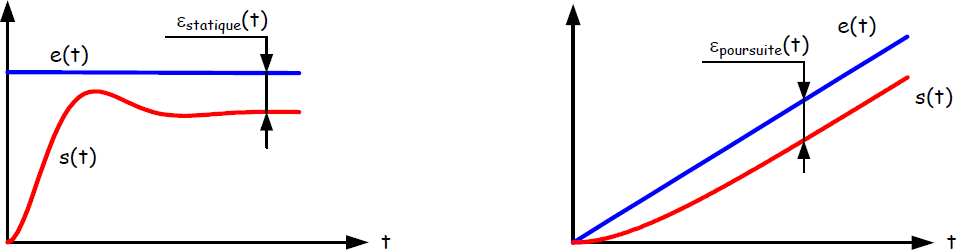
\includegraphics[width=.9\linewidth]{images/fig_erreur}
\end{center}

\subsection*{Petit développement ...}

Calculons l'écart statique pour le système précédent. On a : $\varepsilon(p)=E(p)-R(p)=E(p)-\varepsilon(p) F(p) G(p)$. En conséquences,
$\varepsilon(p)=E(p)-\varepsilon(p) F(p) G(p) 
\Longleftrightarrow \varepsilon(p)\left( 1+F(p) G(p) \right) =E(p) 
\Longleftrightarrow   \varepsilon(p) =\dfrac{E(p)}{1+F(p) G(p)}$.

\begin{resultat}
$$\varepsilon(p) =\dfrac{E(p)}{1+FTBO(p)}$$
\end{resultat}


\subsection*{Poursuivons ...}
On a $FTBO(p)=\dfrac{K_{BO}\left(1+a_1p+...+a_mp^m \right)}{p^{\alpha}\left(1+b_1p+...+b_np^n\right)}$ avec $m< n$.
\subsubsection*{FTBO de classe nulle}

\begin{itemize}
\item Pour une entrée échelon : 
$\varepsilon_{\text{permanent}}=\lim\limits_{p\to 0} p\dfrac{E_0}{p}\dfrac{1}{1+FTBO(p)} 
= \dfrac{E_0}{1+K_{BO}}$.
\item Pour une entrée de type rampe : 
$\varepsilon_{\text{permanent}}=\lim\limits_{p\to 0} p\dfrac{V}{p^2}\dfrac{1}{1+FTBO(p)} 
=+\infty$.
\item Pour une entrée de type parabole : 
$\varepsilon_{\text{permanent}}=\lim\limits_{p\to 0} p\dfrac{A}{p^3}\dfrac{1}{1+FTBO(p)} 
=+\infty$.
\end{itemize}

\subsubsection*{FTBO de classe 1}

\begin{itemize}
\item Pour une entrée échelon : 
$\varepsilon_{\text{permanent}}=\lim\limits_{p\to 0} p\dfrac{E_0}{p}\dfrac{1}{1+\dfrac{K_{BO}\left(1+a_1p+...+a_mp^m \right)}{p\left(1+b_1p+...+b_np^n\right)}} 
= 0$.
\item Pour une entrée de type rampe : 
$\varepsilon_{\text{permanent}}=\lim\limits_{p\to 0} p\dfrac{V}{p^2}\dfrac{1}{1+\dfrac{K_{BO}\left(1+a_1p+...+a_mp^m \right)}{p\left(1+b_1p+...+b_np^n\right)}} 
=\dfrac{V}{K_{BO}}$.
\item Pour une entrée de type parabole : 
$\varepsilon_{\text{permanent}}=\lim\limits_{p\to 0} p\dfrac{A}{p^3}\dfrac{1}{1+\dfrac{K_{BO}\left(1+a_1p+...+a_mp^m \right)}{p\left(1+b_1p+...+b_np^n\right)}} 
=+\infty$.
\end{itemize}

\subsubsection*{FTBO de classe 2}

\begin{itemize}
\item Pour une entrée échelon : 
$\varepsilon_{\text{permanent}}=\lim\limits_{p\to 0} p\dfrac{E_0}{p}\dfrac{1}{1+\dfrac{K_{BO}\left(1+a_1p+...+a_mp^m \right)}{p^{2}\left(1+b_1p+...+b_np^n\right)}} 
= 0$.
\item Pour une entrée de type rampe : 
$\varepsilon_{\text{permanent}}=\lim\limits_{p\to 0} p\dfrac{V}{p^2}\dfrac{1}{1+\dfrac{K_{BO}\left(1+a_1p+...+a_mp^m \right)}{p^{2}\left(1+b_1p+...+b_np^n\right)}} 
=0$.
\item Pour une entrée de type parabole : 
$\varepsilon_{\text{permanent}}=\lim\limits_{p\to 0} p\dfrac{A}{p^3}\dfrac{1}{1+\dfrac{K_{BO}\left(1+a_1p+...+a_mp^m \right)}{p^{2}\left(1+b_1p+...+b_np^n\right)}} 
=\dfrac{A}{K_{BO}}$.
\end{itemize}


\begin{resultat} ~\\

\begin{center}
\begin{tabular}{|c|c|c|c|}
\hline 
Classe & Consigne échelon & Consigne en rampe & Consigne parabolique \\
& $e(t)=E_0$ & $e(t)=V t $ & $e(t)=At^2$ \\ 
& $E(p)=\dfrac{E_0}{p}$ & $E(p)=\dfrac{V}{p^2}$ & $E(p)=\dfrac{A}{p^3}$ \\ 
\hline \hline 
&&&\\
0 & $\varepsilon_S = \dfrac{E_0}{1+K_{BO}} $ & $\varepsilon_V = +\infty$ & $\varepsilon_A = +\infty$ \\
&&&\\
\hline 
&&&\\
1 & $\varepsilon_S = 0$ & $\varepsilon_V = \dfrac{V}{K_{BO}} $ & $\varepsilon_A = +\infty$ \\
&&&\\
\hline 
&&&\\
2 & $\varepsilon_S = 0 $ & $\varepsilon_V = 0$ & $\varepsilon_A = \dfrac{A}{K_{BO}}$ \\
&&&\\
\hline 
\end{tabular}
\end{center}

\begin{rem}
L'écart statique est nul si la boucle ouverte comprend au moins une intégration. À défaut, l'augmentation du gain statique de la boucle ouverte provoque une amélioration de la précision.
\end{rem}

\end{resultat}




%\begin{methode}[Détermination de l'erreur pour un système non perturbé]
%
%\end{methode}

%\begin{methode}[Détermination de l'erreur pour un système perturbé]
%
%\end{methode}
%
%\begin{resultat}
%Tableau...
%\end{resultat}

\section{Système perturbé}
Soit le schéma-blocs suivant : 
\begin{center}
\includestandalone{images/Schema2Entrees_2F_R}
\end{center}

\vspace{.25cm}

\textbf{L'écart est caractérisé par le soustracteur principal, c'est-à-dire celui situé le plus à gauche du schéma-blocs.}

\vspace{.25cm}

Par lecture directe, on a : 
$\varepsilon(p)
=E(p)-R(p)S(p)
=E(p)-R(p)\left(H_2(p) \left(P(p)+\varepsilon(p)H_1(p) \right)\right)$
$\Longleftrightarrow 
\varepsilon(p) =E(p)- R(p)H_2(p)P(p)-R(p)H_1(p)H_2(p)\varepsilon(p) $
$\Longleftrightarrow \varepsilon(p)\left( 1+R(p)H_1(p)H_2(p)\right) =E(p)- R(p)H_2(p)P(p)$
$\Longleftrightarrow \varepsilon(p) =\dfrac{E(p)}{1+R(p)H_1(p)H_2(p)}- \dfrac{R(p)H_2(p)}{1+R(p)H_1(p)H_2(p)}P(p)$.

On a donc :
$\varepsilon(p) =\underbrace{\dfrac{1}{1+\text{FTBO}(p)} E(p)}_{\text{\'Ecart vis-à-vis de la consigne}} - \underbrace{\dfrac{R(p)H_2(p)}{1+\text{FTBO}(p)}P(p)}_{\text{\'Ecart vis-à-vis de la perturbation}}$.

Notons $H_1(p)=\dfrac{K_1}{p^\alpha_1}\dfrac{N_1(p)}{D_1(p)}$ (avec $N_1(0)=1$ et $D_1(0)=1$) et $H_2(p)=\dfrac{K_2}{p^\alpha_2}\dfrac{N_2(p)}{D_2(p)}$ (avec $N_2(0)=1$ et $D_2(0)=1$).

Par ailleurs 
$H_{\text{bo}}(p)=H_1(p)H_2(p)R(p)
=\dfrac{H_{\text{bo}}}{p^{\alpha}}\dfrac{N(p)}{D(p)}$.

On peut calculer l'écart vis-à-vis de la perturbation : 
$\varepsilon_{\text{perturbation}}
= \lim\limits_{t\to\infty}\varepsilon(t)
= \lim\limits_{p\to 0}p \varepsilon(p) 
= \lim\limits_{p\to 0} \dfrac{K_2 p^{\alpha_1+1}}{p^{\alpha_1+\alpha_2}+K_1K_2}P(p) $.

%$S(p)=H_2(p)\left(P(p)+H_1(p)\left(E(p)-R(p)S(p)\right) \right)$
%$=P(p)H_2(p)+H_1(p)H_2(p)E(p)-H_1(p)H_2(p)R(p)S(p)$ 
%$\Leftrightarrow S(p)\left( 1+H_1(p)H_2(p)R(p)\right)=P(p)H_2(p)+H_1(p)H_2(p)E(p)$
%$\Leftrightarrow S(p)=P(p)\dfrac{H_2(p)}{1+H_1(p)H_2(p)R(p)}+\dfrac{H_1(p)H_2(p)}{1+H_1(p)H_2(p)R(p)}E(p)$.

%On a donc $S(p)=P(p)\dfrac{H_2(p)}{1+\text{FTBO}(p)}+\dfrac{H_1(p)H_2(p)}{1+%\text{FTBO}(p)}E(p)$.
\begin{center}
\begin{tabular}{|c|c|c|}
\hline
Cas & Classe du système & Perturbation en échelon $P(p)=\dfrac{P_0}{p}$ \\ \hline
1 & $\alpha_1\geq 1$ & $\varepsilon_{\text{perturbation}}=0$ \\ \hline
2 & $\alpha_1=0$ et $\alpha_2=0$ & $\varepsilon_{\text{perturbation}}=\dfrac{K_2}{1+K_1K_2}P_0$ \\ \hline
3 & $\alpha_1=0$ et $\alpha_2\geq 1$ & $\varepsilon_{\text{perturbation}}=\dfrac{P_0}{K_1}$ \\ \hline
\end{tabular}
\end{center}

\begin{resultat}
Il faut au moins un intégrateur en amont d'une perturbation constante pour
annuler l'écart vis-à-vis de cette perturbation. Un intégrateur placé en aval n'a aucune
influence.

Quand ce n'est pas le cas, un gain $K_1$ important en amont de la perturbation réduit toujours
l'écart vis-à-vis de cette perturbation.
\end{resultat}


\begin{center}
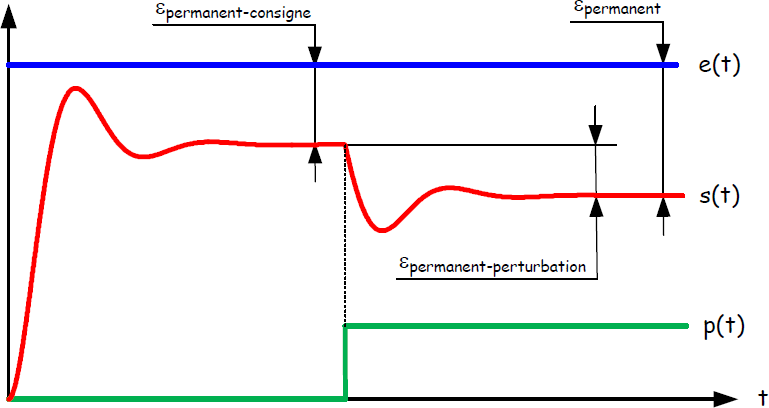
\includegraphics[width=.7\linewidth]{images/fig_erreur_02}
\end{center}


%\section{Précision et réponse fréquentielle}


\begin{thebibliography}{2}
   \bibitem[1]{ref1} Frédéric Mazet, {\it Cours d'automatique de deuxième année, Lycée Dumont Durville, Toulon.}
      \bibitem[2]{ref2} Florestan Mathurin, {\it Précision des SLCI, Lycée Bellevue, Toulouse, \url{http://florestan.mathurin.free.fr/}.}



\end{thebibliography}

\end{document}





% Activation
% Sujet
\newpage
\fichetrue \proffalse \tdtrue \coursfalse
\graphicspath{{../../style/png/}{../../Chapitre_03_Precision/Activation_AssemblageFalcon/images/}}
%%%% Paramétrage du TD %%%%
\def\xxactivite{Activation\ifprof \\ \normalsize \vspace{-.4cm}Corrigé \else \fi}
\def\xxauteur{\textsl{Xavier Pessoles}}


\def\xxnumchapitre{Chapitre 3 \vspace{.2cm}}
\def\xxchapitre{\hspace{.12cm} Précision des systèmes}

\def\xxcompetences{%
\textsl{%
\textbf{Savoirs et compétences :}\\
\vspace{-.4cm}
%\begin{itemize}[label=\ding{112},font=\color{ocre}] 
%%\item \textit{Mod3.C2 : } pôles dominants et réduction de l’ordre du modèle : principe, justification
%%\item \textit{Res2.C4 : } stabilité des SLCI : définition entrée bornée -- sortie bornée (EB -- SB)	
%%\item \textit{Res2.C5 : } stabilité des SLCI : équation caractéristique	
%\item \textit{Res2.C6 : } stabilité des SLCI : position des pôles dans le plan complexe
%\item \textit{Res2.C7 : } stabilité des SLCI : marges de stabilité (de gain et de phase)
%\end{itemize}
}}


\def\xxfigures{
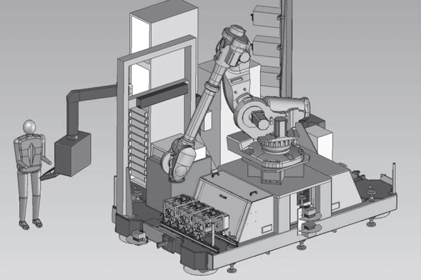
\includegraphics[width=.7\textwidth]{image1}
}%figues de la page de garde

\def\xxtitreexo{Cellule d'assemblage pour avion Falcon}
\def\xxsourceexo{D'après concours E3A -- PSI 2015.}



\iflivret
\pagestyle{empty}


%%%%%%%% PAGE DE GARDE COURS
\ifcours
\begin{tikzpicture}[remember picture,overlay]
\node at (current page.north west)
{\begin{tikzpicture}[remember picture,overlay]
\node[anchor=north west,inner sep=0pt] at (0,0) {\includegraphics[width=\paperwidth]{\thechapterimage}};
\draw[anchor=west] (-2cm,-8cm) node [line width=2pt,rounded corners=15pt,draw=ocre,fill=white,fill opacity=0.6,inner sep=40pt]{\strut\makebox[22cm]{}};
\draw[anchor=west] (1cm,-8cm) node {\huge\sffamily\bfseries\color{black} %
\begin{minipage}{1cm}
\rotatebox{90}{\LARGE\sffamily\textsc{\color{ocre}\textbf{\xxnumpartie}}}
\end{minipage} \hfill
\begin{minipage}[c]{14cm}
\begin{titrepartie}
\begin{flushright}
\renewcommand{\baselinestretch}{1.1} 
\Large\sffamily\textsc{\textbf{\xxpartie}}
\renewcommand{\baselinestretch}{1} 
\end{flushright}
\end{titrepartie}
\end{minipage} \hfill
\begin{minipage}[c]{3.5cm}
{\large\sffamily\textsc{\textbf{\color{ocre} \discipline}}}
\end{minipage} 
 };
\end{tikzpicture}};
\end{tikzpicture}


\begin{tikzpicture}[overlay]
\node[shape=rectangle, 
      rounded corners = .25 cm,
	  draw= ocre,
	  line width=2pt, 
	  fill = ocre!10,
	  minimum width  = 2.5cm,
	  minimum height = 3cm,] at (18cm,0) {};
\node at (17.7cm,0) {\rotatebox{90}{\textbf{\Large\color{ocre}{\classe}}}};
%{};
\end{tikzpicture}

\vspace{3.5cm}

\begin{tikzpicture}[remember picture,overlay]
\draw[anchor=west] (-2cm,-6cm) node {\huge\sffamily\bfseries\color{black} %
\begin{minipage}{2cm}
\begin{center}
\LARGE\sffamily\textsc{\color{ocre}\textbf{\xxactivite}}
\end{center}
\end{minipage} \hfill
\begin{minipage}[c]{15cm}
\begin{titrechapitre}
\renewcommand{\baselinestretch}{1.1} 
\Large\sffamily\textsc{\textbf{\xxnumchapitre}}

\Large\sffamily\textsc{\textbf{\xxchapitre}}
\vspace{.5cm}

\renewcommand{\baselinestretch}{1} 
\normalsize\normalfont
\xxcompetences
\end{titrechapitre}
\end{minipage}  };
\end{tikzpicture}
\vfill

\begin{flushright}
\begin{minipage}[c]{.3\linewidth}
\begin{center}
\xxfigures
\end{center}
\end{minipage}\hfill
\begin{minipage}[c]{.6\linewidth}
\startcontents
\printcontents{}{1}{}
\end{minipage}
\end{flushright}

\begin{tikzpicture}[remember picture,overlay]
\draw[anchor=west] (4.5cm,-.7cm) node {
\begin{minipage}[c]{.2\linewidth}
\begin{flushright}

\includegraphics[width=2cm]{logoCC}
\end{flushright}
\end{minipage}
\begin{minipage}[c]{.2\linewidth}
\textsl{\xxauteur} \\
\textsl{\classe}
\end{minipage}
 };
\end{tikzpicture}
\newpage
\pagestyle{fancy}

\newpage
\pagestyle{fancy}

\else
\fi


%%%%%%%% PAGE DE GARDE TD
\iftd
%\begin{tikzpicture}[remember picture,overlay]
%\node at (current page.north west)
%{\begin{tikzpicture}[remember picture,overlay]
%\draw[anchor=west] (-2cm,-3.25cm) node [line width=2pt,rounded corners=15pt,draw=ocre,fill=white,fill opacity=0.6,inner sep=40pt]{\strut\makebox[22cm]{}};
%\draw[anchor=west] (1cm,-3.25cm) node {\huge\sffamily\bfseries\color{black} %
%\begin{minipage}{1cm}
%\rotatebox{90}{\LARGE\sffamily\textsc{\color{ocre}\textbf{\xxnumpartie}}}
%\end{minipage} \hfill
%\begin{minipage}[c]{13.5cm}
%\begin{titrepartie}
%\begin{flushright}
%\renewcommand{\baselinestretch}{1.1} 
%\Large\sffamily\textsc{\textbf{\xxpartie}}
%\renewcommand{\baselinestretch}{1} 
%\end{flushright}
%\end{titrepartie}
%\end{minipage} \hfill
%\begin{minipage}[c]{3.5cm}
%{\large\sffamily\textsc{\textbf{\color{ocre} \discipline}}}
%\end{minipage} 
% };
%\end{tikzpicture}};
%\end{tikzpicture}

%%%%%%%%%% PAGE DE GARDE TD %%%%%%%%%%%%%%%
%\begin{tikzpicture}[overlay]
%\node[shape=rectangle, 
%      rounded corners = .25 cm,
%	  draw= ocre,
%	  line width=2pt, 
%	  fill = ocre!10,
%	  minimum width  = 2.5cm,
%	  minimum height = 2.5cm,] at (18.5cm,0) {};
%\node at (17.7cm,0) {\rotatebox{90}{\textbf{\Large\color{ocre}{\classe}}}};
%%{};
%\end{tikzpicture}

% PARTIE ET CHAPITRE
%\begin{tikzpicture}[remember picture,overlay]
%\draw[anchor=west] (-1cm,-2.1cm) node {\large\sffamily\bfseries\color{black} %
%\begin{minipage}[c]{15cm}
%\begin{flushleft}
%\xxnumchapitre \\
%\xxchapitre
%\end{flushleft}
%\end{minipage}  };
%\end{tikzpicture}

% Bandeau titre exo
\begin{tikzpicture}[remember picture,overlay]
\draw[anchor=west] (-2cm,-4cm) node {\huge\sffamily\bfseries\color{black} %
\begin{minipage}{5cm}
\begin{center}
\LARGE\sffamily\color{ocre}\textbf{\textsc{\xxactivite}}

\begin{center}
\xxfigures
\end{center}

\end{center}
\end{minipage} \hfill
\begin{minipage}[c]{12cm}
\begin{titrechapitre}
\renewcommand{\baselinestretch}{1.1} 
\large\sffamily\textbf{\textsc{\xxtitreexo}}

\small\sffamily{\textbf{\textit{\color{black!70}\xxsourceexo}}}
\vspace{.5cm}

\renewcommand{\baselinestretch}{1} 
\normalsize\normalfont
\xxcompetences
\end{titrechapitre}
\end{minipage}  };
\end{tikzpicture}

\else
\fi


%%%%%%%% PAGE DE GARDE FICHE
\iffiche
\begin{tikzpicture}[remember picture,overlay]
\node at (current page.north west)
{\begin{tikzpicture}[remember picture,overlay]
\draw[anchor=west] (-2cm,-3.25cm) node [line width=2pt,rounded corners=15pt,draw=ocre,fill=white,fill opacity=0.6,inner sep=40pt]{\strut\makebox[22cm]{}};
\draw[anchor=west] (1cm,-3.25cm) node {\huge\sffamily\bfseries\color{black} %
\begin{minipage}{1cm}
\rotatebox{90}{\LARGE\sffamily\textsc{\color{ocre}\textbf{\xxnumpartie}}}
\end{minipage} \hfill
\begin{minipage}[c]{14cm}
\begin{titrepartie}
\begin{flushright}
\renewcommand{\baselinestretch}{1.1} 
\large\sffamily\textsc{\textbf{\xxpartie} \\} 

\vspace{.2cm}

\normalsize\sffamily\textsc{\textbf{\xxnumchapitre -- \xxchapitre}}
\renewcommand{\baselinestretch}{1} 
\end{flushright}
\end{titrepartie}
\end{minipage} \hfill
\begin{minipage}[c]{3.5cm}
{\large\sffamily\textsc{\textbf{\color{ocre} \discipline}}}
\end{minipage} 
 };
\end{tikzpicture}};
\end{tikzpicture}


\begin{tikzpicture}[overlay]
\node[shape=rectangle, 
      rounded corners = .25 cm,
	  draw= ocre,
	  line width=2pt, 
	  fill = ocre!10,
	  minimum width  = 2.5cm,
	  minimum height = 2.5cm,] at (18.5cm,0.5cm) {};
%	  minimum height = 2.5cm,] at (18.5cm,0cm) {};
\node at (17.7cm,0.5) {\rotatebox{90}{\textsf{\textbf{\large\color{ocre}{\classe}}}}};
%{};
\end{tikzpicture}



\else
\fi



\else
\pagestyle{empty}


%%%%%%%% PAGE DE GARDE COURS
\ifcours
\begin{tikzpicture}[remember picture,overlay]
\node at (current page.north west)
{\begin{tikzpicture}[remember picture,overlay]
\node[anchor=north west,inner sep=0pt] at (0,0) {\includegraphics[width=\paperwidth]{\thechapterimage}};
\draw[anchor=west] (-2cm,-8cm) node [line width=2pt,rounded corners=15pt,draw=ocre,fill=white,fill opacity=0.6,inner sep=40pt]{\strut\makebox[22cm]{}};
\draw[anchor=west] (1cm,-8cm) node {\huge\sffamily\bfseries\color{black} %
\begin{minipage}{1cm}
\rotatebox{90}{\LARGE\sffamily\textsc{\color{ocre}\textbf{\xxnumpartie}}}
\end{minipage} \hfill
\begin{minipage}[c]{14cm}
\begin{titrepartie}
\begin{flushright}
\renewcommand{\baselinestretch}{1.1} 
\Large\sffamily\textsc{\textbf{\xxpartie}}
\renewcommand{\baselinestretch}{1} 
\end{flushright}
\end{titrepartie}
\end{minipage} \hfill
\begin{minipage}[c]{3.5cm}
{\large\sffamily\textsc{\textbf{\color{ocre} \discipline}}}
\end{minipage} 
 };
\end{tikzpicture}};
\end{tikzpicture}


\begin{tikzpicture}[overlay]
\node[shape=rectangle, 
      rounded corners = .25 cm,
	  draw= ocre,
	  line width=2pt, 
	  fill = ocre!10,
	  minimum width  = 2.5cm,
	  minimum height = 3cm,] at (18cm,0) {};
\node at (17.7cm,0) {\rotatebox{90}{\textbf{\Large\color{ocre}{\classe}}}};
%{};
\end{tikzpicture}

\vspace{3.5cm}

\begin{tikzpicture}[remember picture,overlay]
\draw[anchor=west] (-2cm,-6cm) node {\huge\sffamily\bfseries\color{black} %
\begin{minipage}{2cm}
\begin{center}
\LARGE\sffamily\textsc{\color{ocre}\textbf{\xxactivite}}
\end{center}
\end{minipage} \hfill
\begin{minipage}[c]{15cm}
\begin{titrechapitre}
\renewcommand{\baselinestretch}{1.1} 
\Large\sffamily\textsc{\textbf{\xxnumchapitre}}

\Large\sffamily\textsc{\textbf{\xxchapitre}}
\vspace{.5cm}

\renewcommand{\baselinestretch}{1} 
\normalsize\normalfont
\xxcompetences
\end{titrechapitre}
\end{minipage}  };
\end{tikzpicture}
\vfill

\begin{flushright}
\begin{minipage}[c]{.3\linewidth}
\begin{center}
\xxfigures
\end{center}
\end{minipage}\hfill
\begin{minipage}[c]{.6\linewidth}
\startcontents
\printcontents{}{1}{}
\end{minipage}
\end{flushright}

\begin{tikzpicture}[remember picture,overlay]
\draw[anchor=west] (4.5cm,-.7cm) node {
\begin{minipage}[c]{.2\linewidth}
\begin{flushright}

\includegraphics[width=2cm]{logoCC}
\end{flushright}
\end{minipage}
\begin{minipage}[c]{.2\linewidth}
\textsl{\xxauteur} \\
\textsl{\classe}
\end{minipage}
 };
\end{tikzpicture}
\newpage
\pagestyle{fancy}

\newpage
\pagestyle{fancy}

\else
\fi


%%%%%%%% PAGE DE GARDE TD
\iftd
%\begin{tikzpicture}[remember picture,overlay]
%\node at (current page.north west)
%{\begin{tikzpicture}[remember picture,overlay]
%\draw[anchor=west] (-2cm,-3.25cm) node [line width=2pt,rounded corners=15pt,draw=ocre,fill=white,fill opacity=0.6,inner sep=40pt]{\strut\makebox[22cm]{}};
%\draw[anchor=west] (1cm,-3.25cm) node {\huge\sffamily\bfseries\color{black} %
%\begin{minipage}{1cm}
%\rotatebox{90}{\LARGE\sffamily\textsc{\color{ocre}\textbf{\xxnumpartie}}}
%\end{minipage} \hfill
%\begin{minipage}[c]{13.5cm}
%\begin{titrepartie}
%\begin{flushright}
%\renewcommand{\baselinestretch}{1.1} 
%\Large\sffamily\textsc{\textbf{\xxpartie}}
%\renewcommand{\baselinestretch}{1} 
%\end{flushright}
%\end{titrepartie}
%\end{minipage} \hfill
%\begin{minipage}[c]{3.5cm}
%{\large\sffamily\textsc{\textbf{\color{ocre} \discipline}}}
%\end{minipage} 
% };
%\end{tikzpicture}};
%\end{tikzpicture}

%%%%%%%%%% PAGE DE GARDE TD %%%%%%%%%%%%%%%
%\begin{tikzpicture}[overlay]
%\node[shape=rectangle, 
%      rounded corners = .25 cm,
%	  draw= ocre,
%	  line width=2pt, 
%	  fill = ocre!10,
%	  minimum width  = 2.5cm,
%	  minimum height = 2.5cm,] at (18.5cm,0) {};
%\node at (17.7cm,0) {\rotatebox{90}{\textbf{\Large\color{ocre}{\classe}}}};
%%{};
%\end{tikzpicture}

% PARTIE ET CHAPITRE
%\begin{tikzpicture}[remember picture,overlay]
%\draw[anchor=west] (-1cm,-2.1cm) node {\large\sffamily\bfseries\color{black} %
%\begin{minipage}[c]{15cm}
%\begin{flushleft}
%\xxnumchapitre \\
%\xxchapitre
%\end{flushleft}
%\end{minipage}  };
%\end{tikzpicture}

% Bandeau titre exo
\begin{tikzpicture}[remember picture,overlay]
\draw[anchor=west] (-2cm,-4cm) node {\huge\sffamily\bfseries\color{black} %
\begin{minipage}{5cm}
\begin{center}
\LARGE\sffamily\color{ocre}\textbf{\textsc{\xxactivite}}

\begin{center}
\xxfigures
\end{center}

\end{center}
\end{minipage} \hfill
\begin{minipage}[c]{12cm}
\begin{titrechapitre}
\renewcommand{\baselinestretch}{1.1} 
\large\sffamily\textbf{\textsc{\xxtitreexo}}

\small\sffamily{\textbf{\textit{\color{black!70}\xxsourceexo}}}
\vspace{.5cm}

\renewcommand{\baselinestretch}{1} 
\normalsize\normalfont
\xxcompetences
\end{titrechapitre}
\end{minipage}  };
\end{tikzpicture}

\else
\fi


%%%%%%%% PAGE DE GARDE FICHE
\iffiche
\begin{tikzpicture}[remember picture,overlay]
\node at (current page.north west)
{\begin{tikzpicture}[remember picture,overlay]
\draw[anchor=west] (-2cm,-3.25cm) node [line width=2pt,rounded corners=15pt,draw=ocre,fill=white,fill opacity=0.6,inner sep=40pt]{\strut\makebox[22cm]{}};
\draw[anchor=west] (1cm,-3.25cm) node {\huge\sffamily\bfseries\color{black} %
\begin{minipage}{1cm}
\rotatebox{90}{\LARGE\sffamily\textsc{\color{ocre}\textbf{\xxnumpartie}}}
\end{minipage} \hfill
\begin{minipage}[c]{14cm}
\begin{titrepartie}
\begin{flushright}
\renewcommand{\baselinestretch}{1.1} 
\large\sffamily\textsc{\textbf{\xxpartie} \\} 

\vspace{.2cm}

\normalsize\sffamily\textsc{\textbf{\xxnumchapitre -- \xxchapitre}}
\renewcommand{\baselinestretch}{1} 
\end{flushright}
\end{titrepartie}
\end{minipage} \hfill
\begin{minipage}[c]{3.5cm}
{\large\sffamily\textsc{\textbf{\color{ocre} \discipline}}}
\end{minipage} 
 };
\end{tikzpicture}};
\end{tikzpicture}


\begin{tikzpicture}[overlay]
\node[shape=rectangle, 
      rounded corners = .25 cm,
	  draw= ocre,
	  line width=2pt, 
	  fill = ocre!10,
	  minimum width  = 2.5cm,
	  minimum height = 2.5cm,] at (18.5cm,0.5cm) {};
%	  minimum height = 2.5cm,] at (18.5cm,0cm) {};
\node at (17.7cm,0.5) {\rotatebox{90}{\textsf{\textbf{\large\color{ocre}{\classe}}}}};
%{};
\end{tikzpicture}



\else
\fi



\fi
\setlength{\columnseprule}{.1pt}

\pagestyle{fancy}
\thispagestyle{plain}


\vspace{4.5cm}

\def\columnseprulecolor{\color{ocre}}
\setlength{\columnseprule}{0.4pt} 

%%%%%%%%%%%%%%%%%%%%%%%


\begin{multicols}{2}
\setcounter{exo}{0}
\subsection*{Présentation}
Le tronçon central du fuselage du Falcon 7X est assemblé par rivetage grâce à un robot 6 axes. Les rivets sont stockés dans des cassettes rangées verticalement. Un chariot de sélection se déplace verticalement pour déplacer une buse d'aspiration qui permettra d'acheminer les rivets contenus dans la cassette vers l'effecteur (robot). Le chariot fait l'objet de cette étude.

\begin{center}
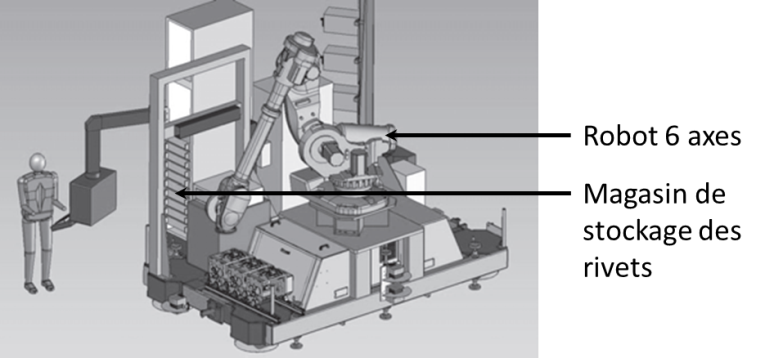
\includegraphics[width=7cm]{image5}
\end{center} 

\begin{obj}
Vérifier que les correcteurs proposés permettent ou non d'obtenir un écart statique nul et un écart en vitesse nul.
\end{obj}
% 
%L'objectif de cette partie est de valider les choix effectués par la société pour le sous ensemble de sélection des fixations de la cellule (exigence 1.1).

%\vfill
%
%\begin{center}
%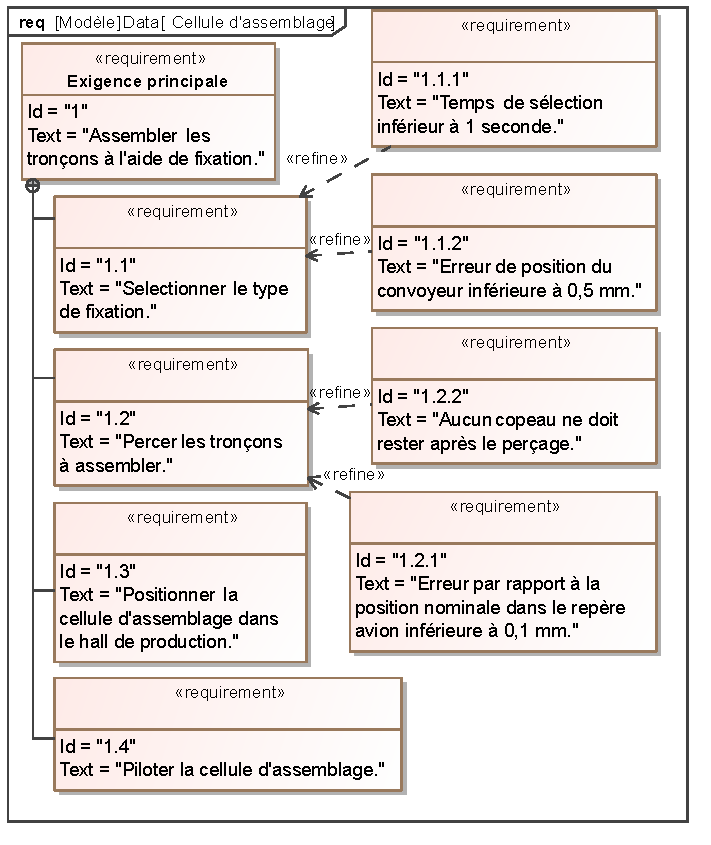
\includegraphics[width=7cm]{Exigences}
%\end{center} 




% 
%\subsection*{Axe chariot}
%Le déplacement du chariot est assuré par un axe numérique asservi en vitesse et en position. Cet axe est composé d'un moteur à courant continu, d'un système de transmission de puissance de type poulies / courroie et d'un rail.
% 
%\begin{center}
%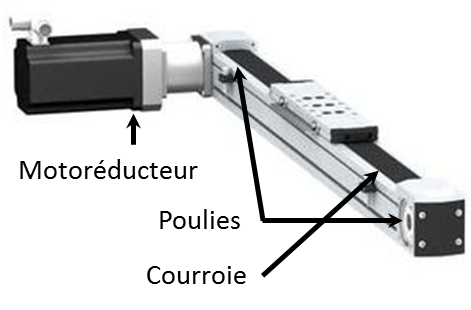
\includegraphics[width=4.5cm]{image7}
%\end{center} 
%
%
%\subsection*{Modélisation du système de déplacement du chariot}
%
%\begin{center}
%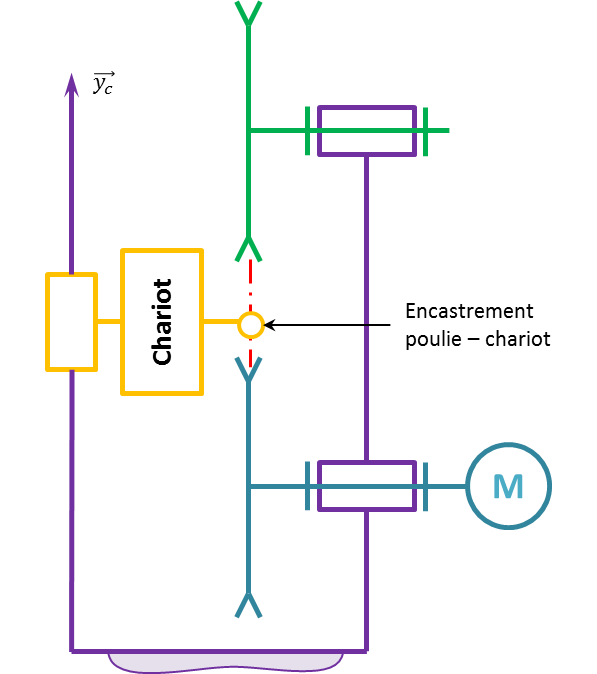
\includegraphics[width=5cm]{image8}
%\end{center} 
%
%
%\fi

%
%
%
%\section*{Sélectionner les fixations – Exigence 1.1}
%\ifprof
%\else 
%Afin de sélectionner le type de fixation, la buse d'aspiration doit être déplacée en face de la cassette avec une erreur inférieure à $\SI{0,5}{mm}$ (voir exigences fonctionnelles). Cependant le fabricant du système poulie-courroie du rail indique déjà une erreur de $\pm \SI{0,25}{mm}$ due notamment à l'élasticité de la courroie. Par conséquent, l'erreur en position de la commande doit être nulle. De plus, afin de ne pas perdre de temps lors de la production, le temps maximal de déplacement lors de la sélection est imposé à une seconde.
%
%L'étude se fera dans le cas le plus défavorable c'est-à-dire un déplacement du chariot vers le haut entre les deux cassettes de rivets les plus éloignées. L'axe de déplacement est appelé $\vect{y_c}$
%\subsection*{Notations domaine temporel – domaine de Laplace}
%
%Les notations entre le domaine temporel et celui de Laplace sont données dans la suite. Ainsi, si la fonction $f(t)$ possède une transformée de Laplace, elle sera notée : $F(p) = \mathcal{L}[f(t)]$.
%Les équations caractéristiques du moteur à courant continu sont rappelées ci-dessous (les conditions de Heaviside sont respectées) :
%\begin{itemize}[label=\ding{112},font=\color{ocre}] 
%\item $u(t)=e(t)+L \dfrac{di(t)}{\text{d} t}+Ri(t)$;
%\item $e(t)=K_E \omega_m (t)$ ;
%\item $C_M (t)=K_C i(t)$ ;
%\item $J_{eq}  \dfrac{d\omega_m)}{\text{d} t}+f\omega_m (t)=C_M (t)-C_R (t)$.
%\end{itemize}
%
%Avec : 
%\begin{itemize}[label=\ding{112},font=\color{ocre}] 
%\item $u(t)$ : tension moteur ;
%\item $i(t)$ : courant moteur ; 
%\item $e(t)$ : force contre-électromotrice ;
%\item $\omega_m(t)$ : vitesse de rotation moteur ;
%\item $C_M (t)$ : couple moteur ;
%\item $C_R (t)$: couple résistant modélisant l'action de pesanteur.
%\end{itemize}
%\fi
%
%\subsection*{Critères à respecter pour l'exigence 1.2}
%\ifprof
%\else
%\footnotesize{
%\begin{center}
%\begin{tabular}{|p{2cm}|p{2.5cm}|p{2cm}|}
%\hline
%Exigence	& Critères & Niveaux \\ \hline
%Déplacer le chariot	& Précision :
%erreur statique par rapport à une consigne de vitesse constante	
%& NULLE \\ \hline
%	& Rapidité : temps de réponse à 5\% en réponse à une consigne échelon 
%	& $Tr_{5\%} = \SI{0,1}{s}$  maxi \\ \hline
%	& Stabilité : & \\
%	& Marge de gain & \SI{6}{dB} mini \\
%	&Marge de gain & $\ang{45}$ mini \\
%\hline
%\end{tabular}
%\end{center}}

%\fi
%\subsection*{Choix d'une architecture de la chaine de transmission}
%\subparagraph{}
%\textit{Proposer sous la forme d'un schéma une autre solution permettant le déplacement du chariot. La conversion de l'énergie électrique en énergie mécanique par un moteur doit être conservée.}
%
%\ifprof
%\begin{corrige}
%Utilisation d’un système vis-écrou.
%\end{corrige}
%\else
%\fi
%
%\ifprof
%\else
%Compte tenu des vitesses de translation importantes, le système retenu est de type poulie-courroie.
%\fi
%
%\subsection*{Détermination de l'inertie équivalente} 
%\ifprof
%\else
%
%Les grandeurs caractéristiques (notations et valeurs) des éléments de l'axe du chariot sont données dans le tableau ci-dessous :
%\begin{center}
%\begin{tabular}{|p{3cm}|c|c|}
%\hline
%Moment d'inertie du rotor du moteur autour de son axe&	$J_m$ & $\num{140d-6}\si{kg.m^2}$ \\ \hline
%Moment d'inertie du réducteur ramené à l'arbre moteur&	$J_{réd}$ & $\num{60d-4}\si{kg.m^2}$ \\ \hline
%Moment d'inertie de la poulie motrice autour de son axe&	$J_{PM}$	&$ \num{38d-4}\si{kg.m^2}$ \\ \hline
%Moment d'inertie de la poulie réceptrice autour de son axe&	$J_{PR}$ & $\num{38d-4}\si{kg.m^2}$ \\ \hline
%Masse totale du chariot	&$M$ &$\SI{5}{kg}$ \\ \hline
%Vitesse de rotation de l'arbre moteur &$\omega_m$ &  \\ \hline
%Vitesse de rotation de l'arbre de sortie du réducteur	&$\omega_r$&  \\ \hline
%Rayon d'une poulie motrice ou réceptrice	& $R_P$ &$\SI{45}{mm}$ \\ \hline
%Rapport de réduction réducteur ($\omega_r/\omega_m$)	& $\lambda$	&$1/5$ \\ \hline
%\end{tabular}
%\end{center}
%\fi
%
%\subparagraph{}
%\textit{À partir des grandeurs définies déterminer l'expression littérale de l'inertie équivalente $J_{eq}$ de l'ensemble $\Sigma=$\{moteur+réducteur+poulies+chariot\} ramenée sur l'arbre moteur. Cette inertie équivalente est définie par $E_c (\Sigma)=1/2 J_{eq} \omega_m^2$.}
%\ifprof
%\begin{corrige}
%$\mathcal{E}_c(\Sigma)=\mathcal{E}_c (\text{moteur})+\mathcal{E}_c (\text{réducteur})+\mathcal{E}_c (\text{poulies})+\mathcal{E}_c (\text{chariot})$.
%\begin{itemize}
%	\item $\mathcal{E}_c (\text{moteur})=1/2 J_m \omega_m^2$;
%	\item $\mathcal{E}_c (\text{réducteur})=1/2 J_{\text{red}} \omega_m^2$;
%	\item $\mathcal{E}_c (\text{poulies})=1/2 (J_{\text{Pm}}+J_{\text{PR}}  ) \omega_{\text{red}}^2=1/2 (J_{\text{Pm}}+J_{\text{PR}}  ) \lambda^2 \omega_m^2$;
%	\item $\mathcal{E}_c (\text{chariot})=1/2 MV^2=1/2 MR_p^2 \lambda^2 \omega_m^2$.
%\end{itemize}
%On a donc $J_{\text{eq}}=MR_p^2 \lambda^2+(J_{\text{Pm}}+J_{\text{PR}}  ) \lambda^2+J_{\text{red}}+J_m$.
%
%\end{corrige}
%\else
%\fi
%
%\subparagraph{}
%\textit{Déterminer la valeur numérique de l'expression précédente.}
%\ifprof
%\begin{corrige}
%$J_{eq}=\SI{0,0068}{kg.m^2}$
%\end{corrige}
%\else
%\fi
%
%\subsection*{Modèle de connaissance du moteur à courant continu}
%
%\begin{obj}
%L'objectif de cette partie est d'établir un modèle de la motorisation de l'axe afin de simuler un déplacement.
%\end{obj}
%
%\subparagraph{}
%\textit{À partir des équations du moteur à courant continu, réaliser le schéma bloc du moteur à courant continu.}
%\ifprof
%\begin{corrige} ~\\
%
%\begin{center}
%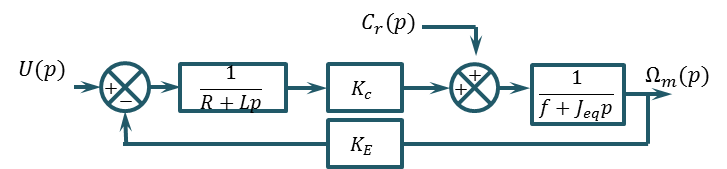
\includegraphics[width=7cm]{corr_01}
%\end{center} 
%\end{corrige}
%\else
%\fi
%
%\subparagraph{}
%\textit{En considérant que $C_R (p)=0$, déterminer la fonction de transfert $H_M (p)=\dfrac{\Omega_m (p)}{U(p)}$ sous sa forme canonique.}
%\ifprof
%\begin{corrige}
%$H_m (p)=\dfrac{\dfrac{K_C}{K_c K_E+Rf}}{1+\dfrac{RJ_eq+Lf}{K_c K_E+Rf}p+\dfrac{LJ_eq}{K_c K_E+Rf} p^2}$
%\end{corrige}
%\else
%\fi
%
%\subparagraph{}
%\textit{Montrer que la fonction de transfert $H_M (p)$ peut se mettre sous la forme $H_M (p)=\dfrac{K_C}{K_C K_e+RJ_{eq} p+LJ_{eq} p^2 }$. Justifier la réponse. Pour cette question, la valeur numérique de $J_{eq}$ considérée sera $J_{eq}=\num{7d-3}\si{kg.m^2}$ indépendamment du résultat numérique calculé précédemment.}
%\ifprof
%\begin{corrige}
%En faisant les applications numériques on montre que $Rf$ est négligeable devant $K_c K_E$ et que $Lf$ et négligeable devant $RJ_{eq}$. On a donc : 
%$H_m (p)=\dfrac{\dfrac{K_C}{K_c K_E}}{1+\dfrac{RJ_{eq}}{K_c K_E }p+\dfrac{LJ_{eq}}{K_c K_E }p^2 }=\dfrac{K_C}{K_c K_E+RJ_{eq} p+LJ_{eq} p^2 }$.
%
%\end{corrige}
%\else
%\fi
%
%\subparagraph{}
%\textit{Montrer qu'avec l'expression, $H_M (p)$ peut s'écrire sous la forme $H_M (p)=\dfrac{K_M}{(1+T_E p)(1+T_M p)}$  avec $T_E<T_M$.}
%\ifprof
%\begin{corrige}
%$
%\left\{
%\begin{array}{l}
%T_e+T_m= \dfrac{RJ_{eq}}{K_c K_e}\\
%T_e T_m=\dfrac{LJ_{eq}}{K_C K_e}
%\end{array}
%\right.
%$
%On a (résolution d’une équation du second degré):
%
%$Te=\dfrac{\dfrac{RJ_{eq}}{K_c K_e}-\sqrt{\left(\dfrac{RJ_{eq}}{K_c K_e}\right)^2 - 4\dfrac{LJ_{eq}}{K_c K_e}}}{2}$. $T_e=\SI{0,0051}{s}$ et $T_m=\SI{0,0074}{s}$.
%
%
%\end{corrige}
%\else
%\fi
%\section*{Étude de l'asservissement en position de l'axe}
%\subsection*{Modélisation de l'asservissement en position}
%\ifprof
%\else
%
%
%La partie précédente a permis de déterminer un modèle du moteur. La suite de l'étude va permettre, par simulation, de déterminer les réglages nécessaires de l'axe vis-à-vis du cahier des charges. La figure suivante présente le principe de l'asservissement de l'axe du chariot.
% 
%\begin{center}
%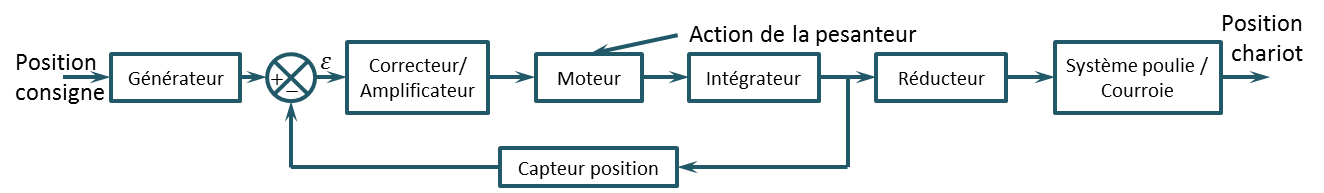
\includegraphics[width=7cm]{image9}
%\end{center} 
%
%Les grandeurs caractéristiques des blocs de l'asservissement de l'axe chariot sont données dans le tableau ci-dessous :
%\begin{center}
%\begin{tabular}{|c|c|c|}
%\hline
%Générateur & $K_G$ & À déterminer \\
%\hline
%Capteur de position	& $K_\text{capt}$ & $\num{5d-3}\si{V.rad^(-1)}$ \\
%\hline
%Correcteur amplificateur	 & $C(p)$ & Variable \\
%\hline
%\end{tabular}
%\end{center}
%\fi
%
%\subparagraph{}
%\textit{Quelle doit être la valeur de $K_G$ pour assurer un asservissement correct (c'est-à-dire l'écart $\varepsilon$ doit être nul si la position de l'axe est identique à la consigne) ?}
%\ifprof
%\begin{corrige} ~\\
%
%On doit avoir $K_G=K_{\text{capt}} \dfrac{1}{\lambda} \dfrac{1}{R_p}=\SI{0,556}{V.rad^{-1}.m^{-1}}$.
%\end{corrige}
%\else
%\fi
%
%\subparagraph{}
%\textit{Donner le schéma-blocs de l'asservissement.}
%\ifprof
%\begin{corrige} ~\\
%
%\begin{center}
%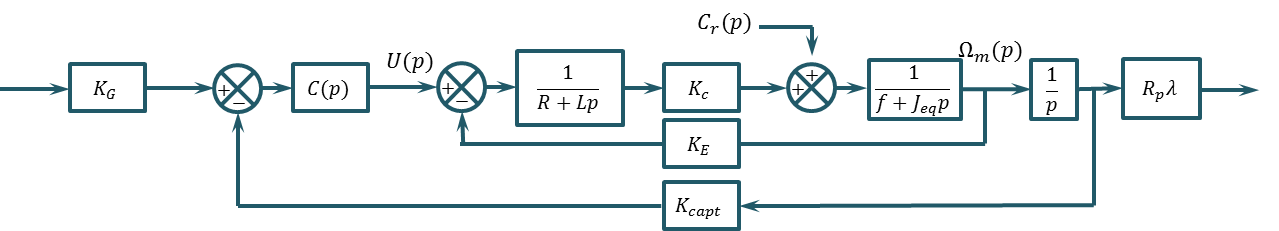
\includegraphics[width=7cm]{corr_02}
%\end{center} 
%
%\end{corrige}
%\else
%\fi

\subsection*{Étude du modèle simplifié}
\ifprof
\else
Afin de faciliter les calculs, le schéma bloc à retour unitaire est donné figure suivante. Le couple résistant $C_r$ dû à l'action de pesanteur est supposé constant.
 
 \begin{center}
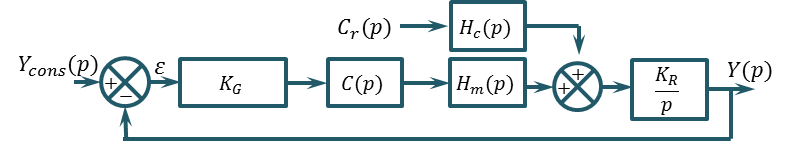
\includegraphics[width=\linewidth]{image10}
\end{center} 


Avec : 

\noindent $H_M (p)=\dfrac{K_M}{(1+T_E p)(1+T_M p)} \text{ et }
H_C (p)=\dfrac{\dfrac{\left(R+Lp\right)K_M}{K_C}}{(1+T_E p)(1+T_M p)}$.
%\item $C_R (p)=C_r/p$;
%\item $K_R=R_p \lambda$.
%\end{itemize}
\fi

\subparagraph{}
\textit{Donner l'expression de $\varepsilon(p)$.}
\ifprof
\begin{corrige}~\\
On raisonne par superposition :

Si $C_r (p)=0$: 

$$Y_1 (p)
=Y_{\text{cons}}(p) \dfrac{\dfrac{K_G K_{\text{Capt}} C(p) H_m (p) K_r}{p}}{1+\dfrac{K_G K_{\text{Capt}} C(p) H_m (p) K_r}{p}}$$

$$
=Y_{\text{cons}} (p) \dfrac{K_G K_{\text{Capt}} C(p) H_m (p) K_r}{p+K_G K_{\text{Capt}} C(p) H_m (p) K_r } 
$$

$$
=Y_{\text{cons}} (p) \dfrac{K_G K_{\text{Capt}} C(p) K_M  K_r}{(1+T_E p)(1+T_M p)p+K_G K_{\text{Capt}} C(p) K_M K_r )}$$.

\end{corrige}

\begin{corrige}
Si $Y_{\text{Cons}} (p)=0$ :

$$Y_2 (p)
=C_r (p) \dfrac{\dfrac{H_c (p) K_r}{p}}{1+\dfrac{K_r K_G K_{\text{Capt}} C(p) H_m (p)}{p} }$$

$$
=C_r (p) \dfrac{H_c (p) K_r}{p+K_r K_G K_{\text{Capt}} C(p) H_m (p) }$$
$$
=C_r (p) \dfrac{\dfrac{(R+Lp) K_M  K_r}{K_C }}{(1+T_E p)(1+T_M p)p+K_r K_G K_{\text{Capt}} C(p) K_M }$$

On a donc :
$Y(p)=Y_1 (p)+Y_2 (p)$.

\end{corrige}
\else
\fi

\subparagraph{}
\textit{On souhaite déterminer l'erreur en position du système. Calculer l'écart statique pour $C(p)=K_p$. Pouvait-on prévoir le résultat ?}
\ifprof
\begin{corrige}
\end{corrige}
\else
\fi


\subparagraph{}
\textit{On souhaite déterminer l'erreur en position du système. Calculer l'écart statique pour $C(p)=\dfrac{K_i}{p}$. Pouvait-on prévoir le résultat ?}
\ifprof
\begin{corrige}
\end{corrige}
\else
\fi


\subparagraph{}
\textit{On souhaite déterminer l'erreur en vitesse du système. Calculer l'erreur pour $C(p)=\dfrac{K_i}{p}$. Pouvait-on prévoir le résultat ?}
\ifprof
\begin{corrige}
\end{corrige}
\else
\fi


\subparagraph{}
\textit{On souhaite déterminer l'erreur pour un entrée en position du système avec une perturbation de type rampe. Calculer l'erreur pour $C(p)=\dfrac{K_i}{p}$. Pouvait-on prévoir le résultat ?}
\ifprof
\begin{corrige}
\end{corrige}
\else
\fi

%
%\subparagraph{}
%\textit{On souhaite que lorsque le système se déplace à vitesse constante, l'erreur sur la vitesse atteinte par le système soit nulle. Quelle sollicitation doit-on utiliser. Calculer l'écart statique pour $C(p)=K_p$ puis $C(p)=\dfrac{K_i}{p}$.}
%\ifprof
%\begin{corrige}
%\end{corrige}
%\else
%\fi
%
%\subparagraph{}
%\textit{Conclure.}
%\ifprof
%\begin{corrige}
%\end{corrige}
%\else
%\fi

%\ifprof
%\else
%
%Afin de répondre totalement au cahier des charges, l'utilisation d'un correcteur proportionnel intégral dérivé est retenue. En effet, la commande de l'axe intègre directement ce type de correcteur. Dans la suite du problème, le correcteur $C(p)$ sera de la forme : $C(p)=K_I \left(1+\dfrac{1}{(T_I p}\right)\left(1+T_D p\right)$. Le réglage des coefficients a été fait par simulation numérique.
%Afin de vérifier maintenant le critère de rapidité, on donne la réponse temporelle (figure page suivante) de l'axe à un échelon de position de $\SI{1}{m}$.
%
%\fi
%
%\subparagraph{}
%\textit{Conclure sur la conformité au cahier des charges du système ainsi réglé.}
%\ifprof
%\begin{corrige}
%\end{corrige}
%\else
%\fi
%
%\ifprof
%\else
% 
% \begin{center}
%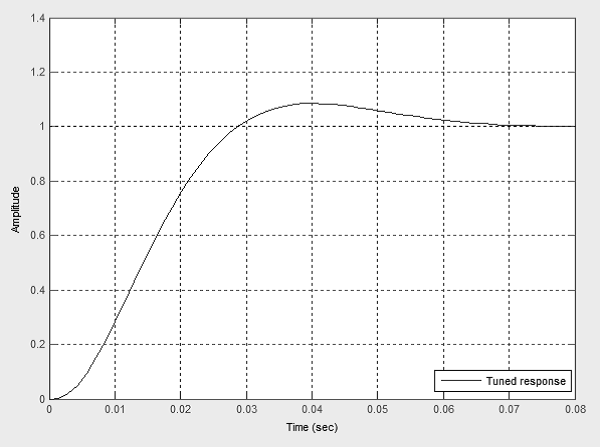
\includegraphics[width=7cm]{image11}
%\end{center} 
%
%\fi
% 
%
%\subparagraph{}
%\textit{Tracer de diagramme de Bode.}
%\ifprof
%\begin{corrige}
%\end{corrige}
%\else
%\fi
%
%\ifprof
%\else
%
%On considère $C_R (p)=0$. On prendra $K_M=\SI{0,8}{rad.s^{-1}.V^{-1}}$, $T_e=\SI{0,0051}{s}$,$T_m=\SI{0,0074}{s}$.
%\fi
%
%\subparagraph{}
%\textit{Tracer le diagramme de Bode de la fonction de transfert en boucle ouverte pour $C(p)=1$. Déterminer les marges de phase et les marges de gain.}
%\ifprof
%\begin{corrige}
%\end{corrige}
%\else
%\fi
% 
%\subparagraph{}
%\textit{Tracer le diagramme de Bode de la fonction de transfert en boucle ouverte pour $C(p)=\dfrac{1}{p}$. Déterminer les marges de phase et les marges de gain.}
%\ifprof
%\begin{corrige}
%\end{corrige}
%\else
%\fi
%
%\ifprof
%\else
%
%On donne ci-dessous les diagrammes de Bode avec les correcteurs optimisés. Déterminer les marges de gain et marges de phase. 
%\fi
%
%\section*{Vérification des performances de l'axe du magasin de rivets}
%\ifprof
%\else
%
%Afin de vérifier les réglages précédents, un essai sur le système réel est réalisé. Une consigne de \SI{2}{m} est donnée. L'absence de système d'acquisition dédié impose un système de mesure extérieur au système réel. C'est un dispositif d'analyse d'image qui est retenu pour ces mesures.
%\fi
%
%\subparagraph{}
%\textit{À partir des relevés ci-dessous, conclure sur le respect des exigences fonctionnelles de l'axe du magasin de stockage des rivets (Exigence 1.1).}
%\ifprof
%\begin{corrige}
%\end{corrige}
%\else
%\fi
 
\end{multicols}
%
%\ifprof
%\else
%
%\begin{center}
%\begin{tabular}{cc}
%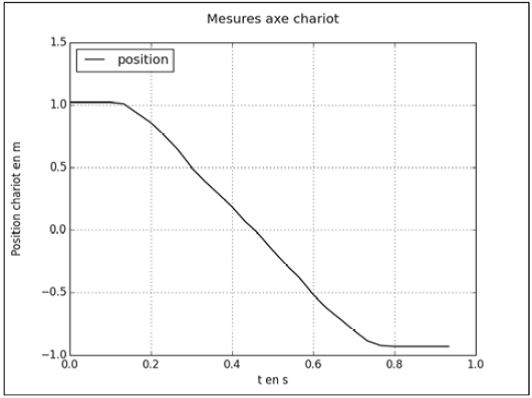
\includegraphics[width=7cm]{image13} &
%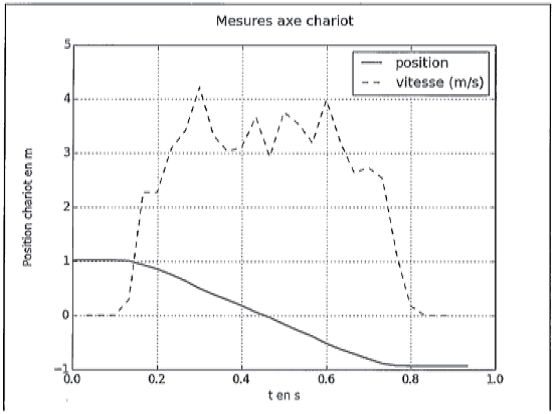
\includegraphics[width=7cm]{image14}
%
%\end{tabular}
%\end{center}
%
% \begin{center}
%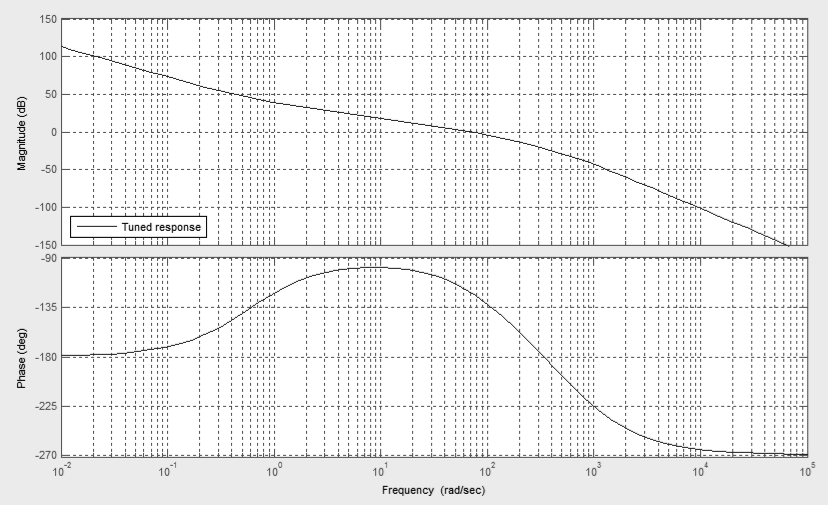
\includegraphics[width=\textwidth]{image12}
%\end{center} 
%\fi

%\end{document}


%%% PAS DE CORRIGE !!!
\newpage
\fichetrue \proftrue \tdtrue \coursfalse
\graphicspath{{../../style/png/}{../../Chapitre_03_Precision/Activation_AssemblageFalcon/images/}}
%%%% Paramétrage du TD %%%%
\def\xxactivite{Activation\ifprof \\ \normalsize \vspace{-.4cm}Corrigé \else \fi}
\def\xxauteur{\textsl{Xavier Pessoles}}


\def\xxnumchapitre{Chapitre 3 \vspace{.2cm}}
\def\xxchapitre{\hspace{.12cm} Précision des systèmes}

\def\xxcompetences{%
\textsl{%
\textbf{Savoirs et compétences :}\\
\vspace{-.4cm}
%\begin{itemize}[label=\ding{112},font=\color{ocre}] 
%%\item \textit{Mod3.C2 : } pôles dominants et réduction de l’ordre du modèle : principe, justification
%%\item \textit{Res2.C4 : } stabilité des SLCI : définition entrée bornée -- sortie bornée (EB -- SB)	
%%\item \textit{Res2.C5 : } stabilité des SLCI : équation caractéristique	
%\item \textit{Res2.C6 : } stabilité des SLCI : position des pôles dans le plan complexe
%\item \textit{Res2.C7 : } stabilité des SLCI : marges de stabilité (de gain et de phase)
%\end{itemize}
}}


\def\xxfigures{
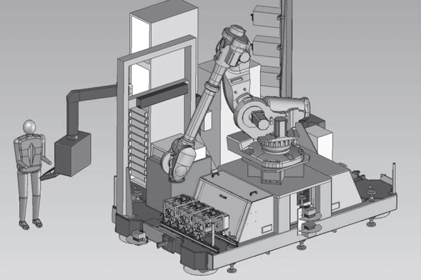
\includegraphics[width=.7\textwidth]{image1}
}%figues de la page de garde

\def\xxtitreexo{Cellule d'assemblage pour avion Falcon}
\def\xxsourceexo{D'après concours E3A -- PSI 2015.}



\iflivret
\pagestyle{empty}


%%%%%%%% PAGE DE GARDE COURS
\ifcours
\begin{tikzpicture}[remember picture,overlay]
\node at (current page.north west)
{\begin{tikzpicture}[remember picture,overlay]
\node[anchor=north west,inner sep=0pt] at (0,0) {\includegraphics[width=\paperwidth]{\thechapterimage}};
\draw[anchor=west] (-2cm,-8cm) node [line width=2pt,rounded corners=15pt,draw=ocre,fill=white,fill opacity=0.6,inner sep=40pt]{\strut\makebox[22cm]{}};
\draw[anchor=west] (1cm,-8cm) node {\huge\sffamily\bfseries\color{black} %
\begin{minipage}{1cm}
\rotatebox{90}{\LARGE\sffamily\textsc{\color{ocre}\textbf{\xxnumpartie}}}
\end{minipage} \hfill
\begin{minipage}[c]{14cm}
\begin{titrepartie}
\begin{flushright}
\renewcommand{\baselinestretch}{1.1} 
\Large\sffamily\textsc{\textbf{\xxpartie}}
\renewcommand{\baselinestretch}{1} 
\end{flushright}
\end{titrepartie}
\end{minipage} \hfill
\begin{minipage}[c]{3.5cm}
{\large\sffamily\textsc{\textbf{\color{ocre} \discipline}}}
\end{minipage} 
 };
\end{tikzpicture}};
\end{tikzpicture}


\begin{tikzpicture}[overlay]
\node[shape=rectangle, 
      rounded corners = .25 cm,
	  draw= ocre,
	  line width=2pt, 
	  fill = ocre!10,
	  minimum width  = 2.5cm,
	  minimum height = 3cm,] at (18cm,0) {};
\node at (17.7cm,0) {\rotatebox{90}{\textbf{\Large\color{ocre}{\classe}}}};
%{};
\end{tikzpicture}

\vspace{3.5cm}

\begin{tikzpicture}[remember picture,overlay]
\draw[anchor=west] (-2cm,-6cm) node {\huge\sffamily\bfseries\color{black} %
\begin{minipage}{2cm}
\begin{center}
\LARGE\sffamily\textsc{\color{ocre}\textbf{\xxactivite}}
\end{center}
\end{minipage} \hfill
\begin{minipage}[c]{15cm}
\begin{titrechapitre}
\renewcommand{\baselinestretch}{1.1} 
\Large\sffamily\textsc{\textbf{\xxnumchapitre}}

\Large\sffamily\textsc{\textbf{\xxchapitre}}
\vspace{.5cm}

\renewcommand{\baselinestretch}{1} 
\normalsize\normalfont
\xxcompetences
\end{titrechapitre}
\end{minipage}  };
\end{tikzpicture}
\vfill

\begin{flushright}
\begin{minipage}[c]{.3\linewidth}
\begin{center}
\xxfigures
\end{center}
\end{minipage}\hfill
\begin{minipage}[c]{.6\linewidth}
\startcontents
\printcontents{}{1}{}
\end{minipage}
\end{flushright}

\begin{tikzpicture}[remember picture,overlay]
\draw[anchor=west] (4.5cm,-.7cm) node {
\begin{minipage}[c]{.2\linewidth}
\begin{flushright}

\includegraphics[width=2cm]{logoCC}
\end{flushright}
\end{minipage}
\begin{minipage}[c]{.2\linewidth}
\textsl{\xxauteur} \\
\textsl{\classe}
\end{minipage}
 };
\end{tikzpicture}
\newpage
\pagestyle{fancy}

\newpage
\pagestyle{fancy}

\else
\fi


%%%%%%%% PAGE DE GARDE TD
\iftd
%\begin{tikzpicture}[remember picture,overlay]
%\node at (current page.north west)
%{\begin{tikzpicture}[remember picture,overlay]
%\draw[anchor=west] (-2cm,-3.25cm) node [line width=2pt,rounded corners=15pt,draw=ocre,fill=white,fill opacity=0.6,inner sep=40pt]{\strut\makebox[22cm]{}};
%\draw[anchor=west] (1cm,-3.25cm) node {\huge\sffamily\bfseries\color{black} %
%\begin{minipage}{1cm}
%\rotatebox{90}{\LARGE\sffamily\textsc{\color{ocre}\textbf{\xxnumpartie}}}
%\end{minipage} \hfill
%\begin{minipage}[c]{13.5cm}
%\begin{titrepartie}
%\begin{flushright}
%\renewcommand{\baselinestretch}{1.1} 
%\Large\sffamily\textsc{\textbf{\xxpartie}}
%\renewcommand{\baselinestretch}{1} 
%\end{flushright}
%\end{titrepartie}
%\end{minipage} \hfill
%\begin{minipage}[c]{3.5cm}
%{\large\sffamily\textsc{\textbf{\color{ocre} \discipline}}}
%\end{minipage} 
% };
%\end{tikzpicture}};
%\end{tikzpicture}

%%%%%%%%%% PAGE DE GARDE TD %%%%%%%%%%%%%%%
%\begin{tikzpicture}[overlay]
%\node[shape=rectangle, 
%      rounded corners = .25 cm,
%	  draw= ocre,
%	  line width=2pt, 
%	  fill = ocre!10,
%	  minimum width  = 2.5cm,
%	  minimum height = 2.5cm,] at (18.5cm,0) {};
%\node at (17.7cm,0) {\rotatebox{90}{\textbf{\Large\color{ocre}{\classe}}}};
%%{};
%\end{tikzpicture}

% PARTIE ET CHAPITRE
%\begin{tikzpicture}[remember picture,overlay]
%\draw[anchor=west] (-1cm,-2.1cm) node {\large\sffamily\bfseries\color{black} %
%\begin{minipage}[c]{15cm}
%\begin{flushleft}
%\xxnumchapitre \\
%\xxchapitre
%\end{flushleft}
%\end{minipage}  };
%\end{tikzpicture}

% Bandeau titre exo
\begin{tikzpicture}[remember picture,overlay]
\draw[anchor=west] (-2cm,-4cm) node {\huge\sffamily\bfseries\color{black} %
\begin{minipage}{5cm}
\begin{center}
\LARGE\sffamily\color{ocre}\textbf{\textsc{\xxactivite}}

\begin{center}
\xxfigures
\end{center}

\end{center}
\end{minipage} \hfill
\begin{minipage}[c]{12cm}
\begin{titrechapitre}
\renewcommand{\baselinestretch}{1.1} 
\large\sffamily\textbf{\textsc{\xxtitreexo}}

\small\sffamily{\textbf{\textit{\color{black!70}\xxsourceexo}}}
\vspace{.5cm}

\renewcommand{\baselinestretch}{1} 
\normalsize\normalfont
\xxcompetences
\end{titrechapitre}
\end{minipage}  };
\end{tikzpicture}

\else
\fi


%%%%%%%% PAGE DE GARDE FICHE
\iffiche
\begin{tikzpicture}[remember picture,overlay]
\node at (current page.north west)
{\begin{tikzpicture}[remember picture,overlay]
\draw[anchor=west] (-2cm,-3.25cm) node [line width=2pt,rounded corners=15pt,draw=ocre,fill=white,fill opacity=0.6,inner sep=40pt]{\strut\makebox[22cm]{}};
\draw[anchor=west] (1cm,-3.25cm) node {\huge\sffamily\bfseries\color{black} %
\begin{minipage}{1cm}
\rotatebox{90}{\LARGE\sffamily\textsc{\color{ocre}\textbf{\xxnumpartie}}}
\end{minipage} \hfill
\begin{minipage}[c]{14cm}
\begin{titrepartie}
\begin{flushright}
\renewcommand{\baselinestretch}{1.1} 
\large\sffamily\textsc{\textbf{\xxpartie} \\} 

\vspace{.2cm}

\normalsize\sffamily\textsc{\textbf{\xxnumchapitre -- \xxchapitre}}
\renewcommand{\baselinestretch}{1} 
\end{flushright}
\end{titrepartie}
\end{minipage} \hfill
\begin{minipage}[c]{3.5cm}
{\large\sffamily\textsc{\textbf{\color{ocre} \discipline}}}
\end{minipage} 
 };
\end{tikzpicture}};
\end{tikzpicture}


\begin{tikzpicture}[overlay]
\node[shape=rectangle, 
      rounded corners = .25 cm,
	  draw= ocre,
	  line width=2pt, 
	  fill = ocre!10,
	  minimum width  = 2.5cm,
	  minimum height = 2.5cm,] at (18.5cm,0.5cm) {};
%	  minimum height = 2.5cm,] at (18.5cm,0cm) {};
\node at (17.7cm,0.5) {\rotatebox{90}{\textsf{\textbf{\large\color{ocre}{\classe}}}}};
%{};
\end{tikzpicture}



\else
\fi



\else
\pagestyle{empty}


%%%%%%%% PAGE DE GARDE COURS
\ifcours
\begin{tikzpicture}[remember picture,overlay]
\node at (current page.north west)
{\begin{tikzpicture}[remember picture,overlay]
\node[anchor=north west,inner sep=0pt] at (0,0) {\includegraphics[width=\paperwidth]{\thechapterimage}};
\draw[anchor=west] (-2cm,-8cm) node [line width=2pt,rounded corners=15pt,draw=ocre,fill=white,fill opacity=0.6,inner sep=40pt]{\strut\makebox[22cm]{}};
\draw[anchor=west] (1cm,-8cm) node {\huge\sffamily\bfseries\color{black} %
\begin{minipage}{1cm}
\rotatebox{90}{\LARGE\sffamily\textsc{\color{ocre}\textbf{\xxnumpartie}}}
\end{minipage} \hfill
\begin{minipage}[c]{14cm}
\begin{titrepartie}
\begin{flushright}
\renewcommand{\baselinestretch}{1.1} 
\Large\sffamily\textsc{\textbf{\xxpartie}}
\renewcommand{\baselinestretch}{1} 
\end{flushright}
\end{titrepartie}
\end{minipage} \hfill
\begin{minipage}[c]{3.5cm}
{\large\sffamily\textsc{\textbf{\color{ocre} \discipline}}}
\end{minipage} 
 };
\end{tikzpicture}};
\end{tikzpicture}


\begin{tikzpicture}[overlay]
\node[shape=rectangle, 
      rounded corners = .25 cm,
	  draw= ocre,
	  line width=2pt, 
	  fill = ocre!10,
	  minimum width  = 2.5cm,
	  minimum height = 3cm,] at (18cm,0) {};
\node at (17.7cm,0) {\rotatebox{90}{\textbf{\Large\color{ocre}{\classe}}}};
%{};
\end{tikzpicture}

\vspace{3.5cm}

\begin{tikzpicture}[remember picture,overlay]
\draw[anchor=west] (-2cm,-6cm) node {\huge\sffamily\bfseries\color{black} %
\begin{minipage}{2cm}
\begin{center}
\LARGE\sffamily\textsc{\color{ocre}\textbf{\xxactivite}}
\end{center}
\end{minipage} \hfill
\begin{minipage}[c]{15cm}
\begin{titrechapitre}
\renewcommand{\baselinestretch}{1.1} 
\Large\sffamily\textsc{\textbf{\xxnumchapitre}}

\Large\sffamily\textsc{\textbf{\xxchapitre}}
\vspace{.5cm}

\renewcommand{\baselinestretch}{1} 
\normalsize\normalfont
\xxcompetences
\end{titrechapitre}
\end{minipage}  };
\end{tikzpicture}
\vfill

\begin{flushright}
\begin{minipage}[c]{.3\linewidth}
\begin{center}
\xxfigures
\end{center}
\end{minipage}\hfill
\begin{minipage}[c]{.6\linewidth}
\startcontents
\printcontents{}{1}{}
\end{minipage}
\end{flushright}

\begin{tikzpicture}[remember picture,overlay]
\draw[anchor=west] (4.5cm,-.7cm) node {
\begin{minipage}[c]{.2\linewidth}
\begin{flushright}

\includegraphics[width=2cm]{logoCC}
\end{flushright}
\end{minipage}
\begin{minipage}[c]{.2\linewidth}
\textsl{\xxauteur} \\
\textsl{\classe}
\end{minipage}
 };
\end{tikzpicture}
\newpage
\pagestyle{fancy}

\newpage
\pagestyle{fancy}

\else
\fi


%%%%%%%% PAGE DE GARDE TD
\iftd
%\begin{tikzpicture}[remember picture,overlay]
%\node at (current page.north west)
%{\begin{tikzpicture}[remember picture,overlay]
%\draw[anchor=west] (-2cm,-3.25cm) node [line width=2pt,rounded corners=15pt,draw=ocre,fill=white,fill opacity=0.6,inner sep=40pt]{\strut\makebox[22cm]{}};
%\draw[anchor=west] (1cm,-3.25cm) node {\huge\sffamily\bfseries\color{black} %
%\begin{minipage}{1cm}
%\rotatebox{90}{\LARGE\sffamily\textsc{\color{ocre}\textbf{\xxnumpartie}}}
%\end{minipage} \hfill
%\begin{minipage}[c]{13.5cm}
%\begin{titrepartie}
%\begin{flushright}
%\renewcommand{\baselinestretch}{1.1} 
%\Large\sffamily\textsc{\textbf{\xxpartie}}
%\renewcommand{\baselinestretch}{1} 
%\end{flushright}
%\end{titrepartie}
%\end{minipage} \hfill
%\begin{minipage}[c]{3.5cm}
%{\large\sffamily\textsc{\textbf{\color{ocre} \discipline}}}
%\end{minipage} 
% };
%\end{tikzpicture}};
%\end{tikzpicture}

%%%%%%%%%% PAGE DE GARDE TD %%%%%%%%%%%%%%%
%\begin{tikzpicture}[overlay]
%\node[shape=rectangle, 
%      rounded corners = .25 cm,
%	  draw= ocre,
%	  line width=2pt, 
%	  fill = ocre!10,
%	  minimum width  = 2.5cm,
%	  minimum height = 2.5cm,] at (18.5cm,0) {};
%\node at (17.7cm,0) {\rotatebox{90}{\textbf{\Large\color{ocre}{\classe}}}};
%%{};
%\end{tikzpicture}

% PARTIE ET CHAPITRE
%\begin{tikzpicture}[remember picture,overlay]
%\draw[anchor=west] (-1cm,-2.1cm) node {\large\sffamily\bfseries\color{black} %
%\begin{minipage}[c]{15cm}
%\begin{flushleft}
%\xxnumchapitre \\
%\xxchapitre
%\end{flushleft}
%\end{minipage}  };
%\end{tikzpicture}

% Bandeau titre exo
\begin{tikzpicture}[remember picture,overlay]
\draw[anchor=west] (-2cm,-4cm) node {\huge\sffamily\bfseries\color{black} %
\begin{minipage}{5cm}
\begin{center}
\LARGE\sffamily\color{ocre}\textbf{\textsc{\xxactivite}}

\begin{center}
\xxfigures
\end{center}

\end{center}
\end{minipage} \hfill
\begin{minipage}[c]{12cm}
\begin{titrechapitre}
\renewcommand{\baselinestretch}{1.1} 
\large\sffamily\textbf{\textsc{\xxtitreexo}}

\small\sffamily{\textbf{\textit{\color{black!70}\xxsourceexo}}}
\vspace{.5cm}

\renewcommand{\baselinestretch}{1} 
\normalsize\normalfont
\xxcompetences
\end{titrechapitre}
\end{minipage}  };
\end{tikzpicture}

\else
\fi


%%%%%%%% PAGE DE GARDE FICHE
\iffiche
\begin{tikzpicture}[remember picture,overlay]
\node at (current page.north west)
{\begin{tikzpicture}[remember picture,overlay]
\draw[anchor=west] (-2cm,-3.25cm) node [line width=2pt,rounded corners=15pt,draw=ocre,fill=white,fill opacity=0.6,inner sep=40pt]{\strut\makebox[22cm]{}};
\draw[anchor=west] (1cm,-3.25cm) node {\huge\sffamily\bfseries\color{black} %
\begin{minipage}{1cm}
\rotatebox{90}{\LARGE\sffamily\textsc{\color{ocre}\textbf{\xxnumpartie}}}
\end{minipage} \hfill
\begin{minipage}[c]{14cm}
\begin{titrepartie}
\begin{flushright}
\renewcommand{\baselinestretch}{1.1} 
\large\sffamily\textsc{\textbf{\xxpartie} \\} 

\vspace{.2cm}

\normalsize\sffamily\textsc{\textbf{\xxnumchapitre -- \xxchapitre}}
\renewcommand{\baselinestretch}{1} 
\end{flushright}
\end{titrepartie}
\end{minipage} \hfill
\begin{minipage}[c]{3.5cm}
{\large\sffamily\textsc{\textbf{\color{ocre} \discipline}}}
\end{minipage} 
 };
\end{tikzpicture}};
\end{tikzpicture}


\begin{tikzpicture}[overlay]
\node[shape=rectangle, 
      rounded corners = .25 cm,
	  draw= ocre,
	  line width=2pt, 
	  fill = ocre!10,
	  minimum width  = 2.5cm,
	  minimum height = 2.5cm,] at (18.5cm,0.5cm) {};
%	  minimum height = 2.5cm,] at (18.5cm,0cm) {};
\node at (17.7cm,0.5) {\rotatebox{90}{\textsf{\textbf{\large\color{ocre}{\classe}}}}};
%{};
\end{tikzpicture}



\else
\fi



\fi
\setlength{\columnseprule}{.1pt}

\pagestyle{fancy}
\thispagestyle{plain}


\vspace{4.5cm}

\def\columnseprulecolor{\color{ocre}}
\setlength{\columnseprule}{0.4pt} 

%%%%%%%%%%%%%%%%%%%%%%%


\begin{multicols}{2}
\setcounter{exo}{0}
\subsection*{Présentation}
Le tronçon central du fuselage du Falcon 7X est assemblé par rivetage grâce à un robot 6 axes. Les rivets sont stockés dans des cassettes rangées verticalement. Un chariot de sélection se déplace verticalement pour déplacer une buse d'aspiration qui permettra d'acheminer les rivets contenus dans la cassette vers l'effecteur (robot). Le chariot fait l'objet de cette étude.

\begin{center}
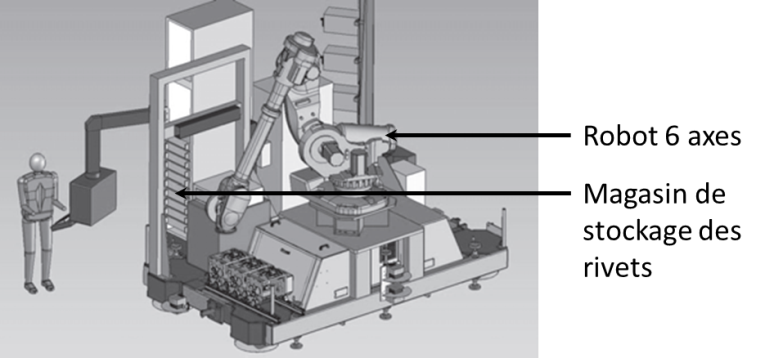
\includegraphics[width=7cm]{image5}
\end{center} 

\begin{obj}
Vérifier que les correcteurs proposés permettent ou non d'obtenir un écart statique nul et un écart en vitesse nul.
\end{obj}
% 
%L'objectif de cette partie est de valider les choix effectués par la société pour le sous ensemble de sélection des fixations de la cellule (exigence 1.1).

%\vfill
%
%\begin{center}
%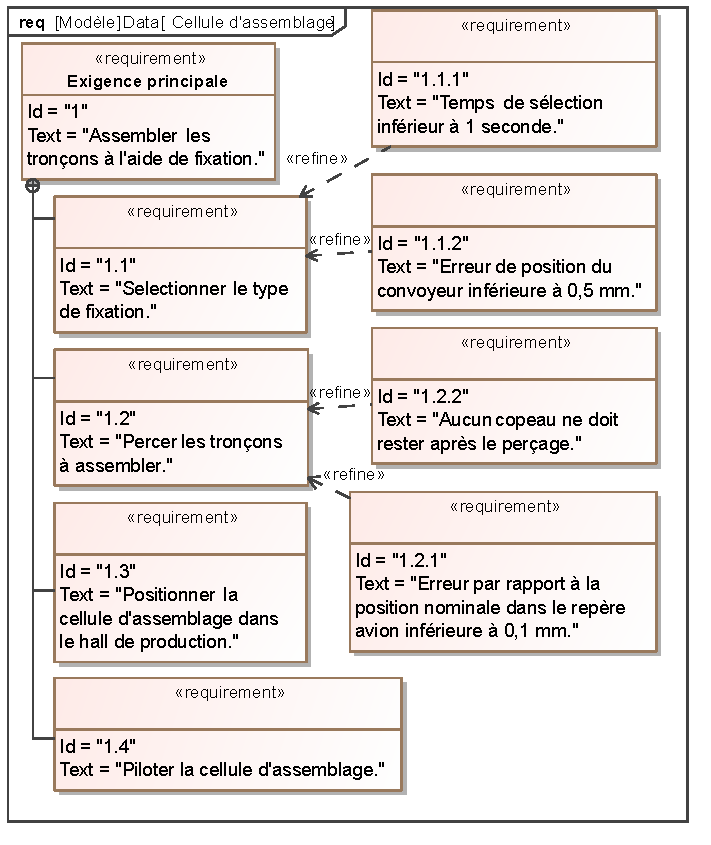
\includegraphics[width=7cm]{Exigences}
%\end{center} 




% 
%\subsection*{Axe chariot}
%Le déplacement du chariot est assuré par un axe numérique asservi en vitesse et en position. Cet axe est composé d'un moteur à courant continu, d'un système de transmission de puissance de type poulies / courroie et d'un rail.
% 
%\begin{center}
%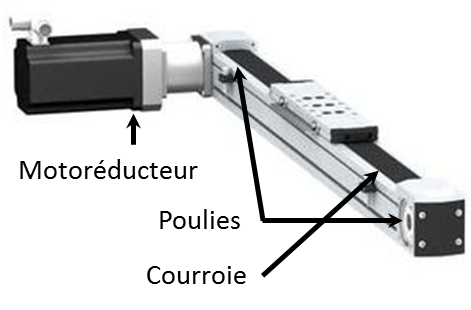
\includegraphics[width=4.5cm]{image7}
%\end{center} 
%
%
%\subsection*{Modélisation du système de déplacement du chariot}
%
%\begin{center}
%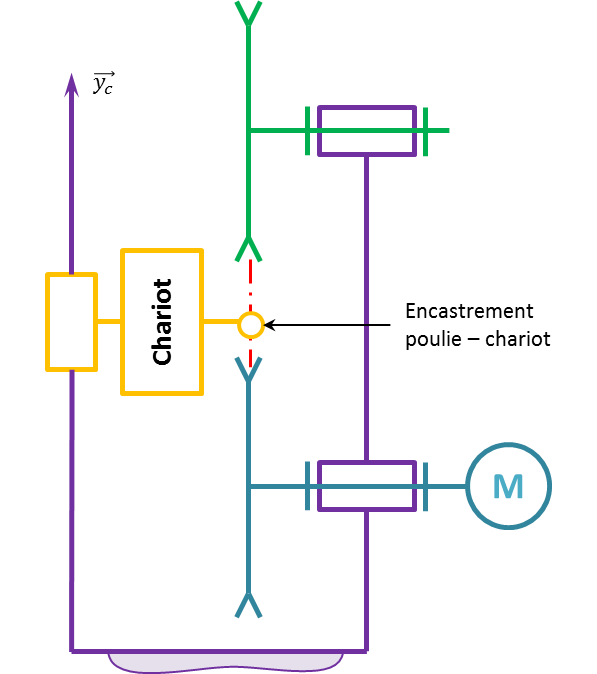
\includegraphics[width=5cm]{image8}
%\end{center} 
%
%
%\fi

%
%
%
%\section*{Sélectionner les fixations – Exigence 1.1}
%\ifprof
%\else 
%Afin de sélectionner le type de fixation, la buse d'aspiration doit être déplacée en face de la cassette avec une erreur inférieure à $\SI{0,5}{mm}$ (voir exigences fonctionnelles). Cependant le fabricant du système poulie-courroie du rail indique déjà une erreur de $\pm \SI{0,25}{mm}$ due notamment à l'élasticité de la courroie. Par conséquent, l'erreur en position de la commande doit être nulle. De plus, afin de ne pas perdre de temps lors de la production, le temps maximal de déplacement lors de la sélection est imposé à une seconde.
%
%L'étude se fera dans le cas le plus défavorable c'est-à-dire un déplacement du chariot vers le haut entre les deux cassettes de rivets les plus éloignées. L'axe de déplacement est appelé $\vect{y_c}$
%\subsection*{Notations domaine temporel – domaine de Laplace}
%
%Les notations entre le domaine temporel et celui de Laplace sont données dans la suite. Ainsi, si la fonction $f(t)$ possède une transformée de Laplace, elle sera notée : $F(p) = \mathcal{L}[f(t)]$.
%Les équations caractéristiques du moteur à courant continu sont rappelées ci-dessous (les conditions de Heaviside sont respectées) :
%\begin{itemize}[label=\ding{112},font=\color{ocre}] 
%\item $u(t)=e(t)+L \dfrac{di(t)}{\text{d} t}+Ri(t)$;
%\item $e(t)=K_E \omega_m (t)$ ;
%\item $C_M (t)=K_C i(t)$ ;
%\item $J_{eq}  \dfrac{d\omega_m)}{\text{d} t}+f\omega_m (t)=C_M (t)-C_R (t)$.
%\end{itemize}
%
%Avec : 
%\begin{itemize}[label=\ding{112},font=\color{ocre}] 
%\item $u(t)$ : tension moteur ;
%\item $i(t)$ : courant moteur ; 
%\item $e(t)$ : force contre-électromotrice ;
%\item $\omega_m(t)$ : vitesse de rotation moteur ;
%\item $C_M (t)$ : couple moteur ;
%\item $C_R (t)$: couple résistant modélisant l'action de pesanteur.
%\end{itemize}
%\fi
%
%\subsection*{Critères à respecter pour l'exigence 1.2}
%\ifprof
%\else
%\footnotesize{
%\begin{center}
%\begin{tabular}{|p{2cm}|p{2.5cm}|p{2cm}|}
%\hline
%Exigence	& Critères & Niveaux \\ \hline
%Déplacer le chariot	& Précision :
%erreur statique par rapport à une consigne de vitesse constante	
%& NULLE \\ \hline
%	& Rapidité : temps de réponse à 5\% en réponse à une consigne échelon 
%	& $Tr_{5\%} = \SI{0,1}{s}$  maxi \\ \hline
%	& Stabilité : & \\
%	& Marge de gain & \SI{6}{dB} mini \\
%	&Marge de gain & $\ang{45}$ mini \\
%\hline
%\end{tabular}
%\end{center}}

%\fi
%\subsection*{Choix d'une architecture de la chaine de transmission}
%\subparagraph{}
%\textit{Proposer sous la forme d'un schéma une autre solution permettant le déplacement du chariot. La conversion de l'énergie électrique en énergie mécanique par un moteur doit être conservée.}
%
%\ifprof
%\begin{corrige}
%Utilisation d’un système vis-écrou.
%\end{corrige}
%\else
%\fi
%
%\ifprof
%\else
%Compte tenu des vitesses de translation importantes, le système retenu est de type poulie-courroie.
%\fi
%
%\subsection*{Détermination de l'inertie équivalente} 
%\ifprof
%\else
%
%Les grandeurs caractéristiques (notations et valeurs) des éléments de l'axe du chariot sont données dans le tableau ci-dessous :
%\begin{center}
%\begin{tabular}{|p{3cm}|c|c|}
%\hline
%Moment d'inertie du rotor du moteur autour de son axe&	$J_m$ & $\num{140d-6}\si{kg.m^2}$ \\ \hline
%Moment d'inertie du réducteur ramené à l'arbre moteur&	$J_{réd}$ & $\num{60d-4}\si{kg.m^2}$ \\ \hline
%Moment d'inertie de la poulie motrice autour de son axe&	$J_{PM}$	&$ \num{38d-4}\si{kg.m^2}$ \\ \hline
%Moment d'inertie de la poulie réceptrice autour de son axe&	$J_{PR}$ & $\num{38d-4}\si{kg.m^2}$ \\ \hline
%Masse totale du chariot	&$M$ &$\SI{5}{kg}$ \\ \hline
%Vitesse de rotation de l'arbre moteur &$\omega_m$ &  \\ \hline
%Vitesse de rotation de l'arbre de sortie du réducteur	&$\omega_r$&  \\ \hline
%Rayon d'une poulie motrice ou réceptrice	& $R_P$ &$\SI{45}{mm}$ \\ \hline
%Rapport de réduction réducteur ($\omega_r/\omega_m$)	& $\lambda$	&$1/5$ \\ \hline
%\end{tabular}
%\end{center}
%\fi
%
%\subparagraph{}
%\textit{À partir des grandeurs définies déterminer l'expression littérale de l'inertie équivalente $J_{eq}$ de l'ensemble $\Sigma=$\{moteur+réducteur+poulies+chariot\} ramenée sur l'arbre moteur. Cette inertie équivalente est définie par $E_c (\Sigma)=1/2 J_{eq} \omega_m^2$.}
%\ifprof
%\begin{corrige}
%$\mathcal{E}_c(\Sigma)=\mathcal{E}_c (\text{moteur})+\mathcal{E}_c (\text{réducteur})+\mathcal{E}_c (\text{poulies})+\mathcal{E}_c (\text{chariot})$.
%\begin{itemize}
%	\item $\mathcal{E}_c (\text{moteur})=1/2 J_m \omega_m^2$;
%	\item $\mathcal{E}_c (\text{réducteur})=1/2 J_{\text{red}} \omega_m^2$;
%	\item $\mathcal{E}_c (\text{poulies})=1/2 (J_{\text{Pm}}+J_{\text{PR}}  ) \omega_{\text{red}}^2=1/2 (J_{\text{Pm}}+J_{\text{PR}}  ) \lambda^2 \omega_m^2$;
%	\item $\mathcal{E}_c (\text{chariot})=1/2 MV^2=1/2 MR_p^2 \lambda^2 \omega_m^2$.
%\end{itemize}
%On a donc $J_{\text{eq}}=MR_p^2 \lambda^2+(J_{\text{Pm}}+J_{\text{PR}}  ) \lambda^2+J_{\text{red}}+J_m$.
%
%\end{corrige}
%\else
%\fi
%
%\subparagraph{}
%\textit{Déterminer la valeur numérique de l'expression précédente.}
%\ifprof
%\begin{corrige}
%$J_{eq}=\SI{0,0068}{kg.m^2}$
%\end{corrige}
%\else
%\fi
%
%\subsection*{Modèle de connaissance du moteur à courant continu}
%
%\begin{obj}
%L'objectif de cette partie est d'établir un modèle de la motorisation de l'axe afin de simuler un déplacement.
%\end{obj}
%
%\subparagraph{}
%\textit{À partir des équations du moteur à courant continu, réaliser le schéma bloc du moteur à courant continu.}
%\ifprof
%\begin{corrige} ~\\
%
%\begin{center}
%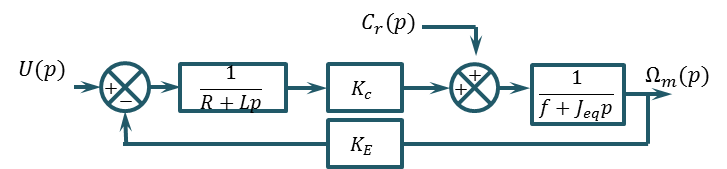
\includegraphics[width=7cm]{corr_01}
%\end{center} 
%\end{corrige}
%\else
%\fi
%
%\subparagraph{}
%\textit{En considérant que $C_R (p)=0$, déterminer la fonction de transfert $H_M (p)=\dfrac{\Omega_m (p)}{U(p)}$ sous sa forme canonique.}
%\ifprof
%\begin{corrige}
%$H_m (p)=\dfrac{\dfrac{K_C}{K_c K_E+Rf}}{1+\dfrac{RJ_eq+Lf}{K_c K_E+Rf}p+\dfrac{LJ_eq}{K_c K_E+Rf} p^2}$
%\end{corrige}
%\else
%\fi
%
%\subparagraph{}
%\textit{Montrer que la fonction de transfert $H_M (p)$ peut se mettre sous la forme $H_M (p)=\dfrac{K_C}{K_C K_e+RJ_{eq} p+LJ_{eq} p^2 }$. Justifier la réponse. Pour cette question, la valeur numérique de $J_{eq}$ considérée sera $J_{eq}=\num{7d-3}\si{kg.m^2}$ indépendamment du résultat numérique calculé précédemment.}
%\ifprof
%\begin{corrige}
%En faisant les applications numériques on montre que $Rf$ est négligeable devant $K_c K_E$ et que $Lf$ et négligeable devant $RJ_{eq}$. On a donc : 
%$H_m (p)=\dfrac{\dfrac{K_C}{K_c K_E}}{1+\dfrac{RJ_{eq}}{K_c K_E }p+\dfrac{LJ_{eq}}{K_c K_E }p^2 }=\dfrac{K_C}{K_c K_E+RJ_{eq} p+LJ_{eq} p^2 }$.
%
%\end{corrige}
%\else
%\fi
%
%\subparagraph{}
%\textit{Montrer qu'avec l'expression, $H_M (p)$ peut s'écrire sous la forme $H_M (p)=\dfrac{K_M}{(1+T_E p)(1+T_M p)}$  avec $T_E<T_M$.}
%\ifprof
%\begin{corrige}
%$
%\left\{
%\begin{array}{l}
%T_e+T_m= \dfrac{RJ_{eq}}{K_c K_e}\\
%T_e T_m=\dfrac{LJ_{eq}}{K_C K_e}
%\end{array}
%\right.
%$
%On a (résolution d’une équation du second degré):
%
%$Te=\dfrac{\dfrac{RJ_{eq}}{K_c K_e}-\sqrt{\left(\dfrac{RJ_{eq}}{K_c K_e}\right)^2 - 4\dfrac{LJ_{eq}}{K_c K_e}}}{2}$. $T_e=\SI{0,0051}{s}$ et $T_m=\SI{0,0074}{s}$.
%
%
%\end{corrige}
%\else
%\fi
%\section*{Étude de l'asservissement en position de l'axe}
%\subsection*{Modélisation de l'asservissement en position}
%\ifprof
%\else
%
%
%La partie précédente a permis de déterminer un modèle du moteur. La suite de l'étude va permettre, par simulation, de déterminer les réglages nécessaires de l'axe vis-à-vis du cahier des charges. La figure suivante présente le principe de l'asservissement de l'axe du chariot.
% 
%\begin{center}
%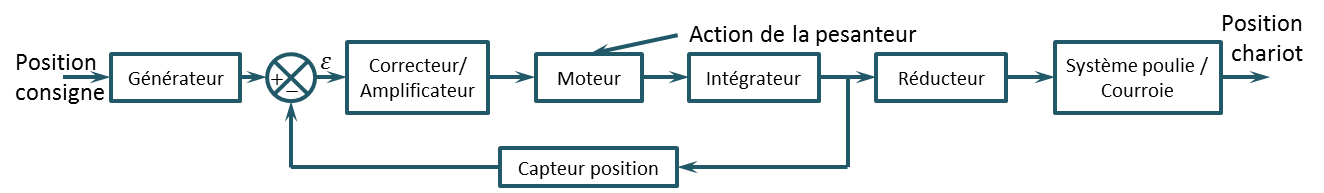
\includegraphics[width=7cm]{image9}
%\end{center} 
%
%Les grandeurs caractéristiques des blocs de l'asservissement de l'axe chariot sont données dans le tableau ci-dessous :
%\begin{center}
%\begin{tabular}{|c|c|c|}
%\hline
%Générateur & $K_G$ & À déterminer \\
%\hline
%Capteur de position	& $K_\text{capt}$ & $\num{5d-3}\si{V.rad^(-1)}$ \\
%\hline
%Correcteur amplificateur	 & $C(p)$ & Variable \\
%\hline
%\end{tabular}
%\end{center}
%\fi
%
%\subparagraph{}
%\textit{Quelle doit être la valeur de $K_G$ pour assurer un asservissement correct (c'est-à-dire l'écart $\varepsilon$ doit être nul si la position de l'axe est identique à la consigne) ?}
%\ifprof
%\begin{corrige} ~\\
%
%On doit avoir $K_G=K_{\text{capt}} \dfrac{1}{\lambda} \dfrac{1}{R_p}=\SI{0,556}{V.rad^{-1}.m^{-1}}$.
%\end{corrige}
%\else
%\fi
%
%\subparagraph{}
%\textit{Donner le schéma-blocs de l'asservissement.}
%\ifprof
%\begin{corrige} ~\\
%
%\begin{center}
%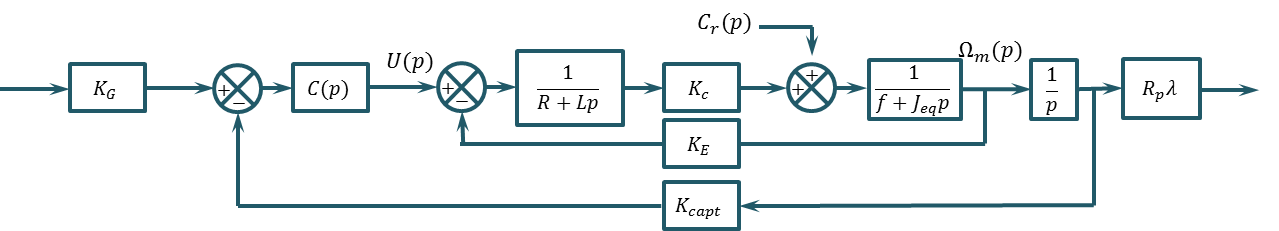
\includegraphics[width=7cm]{corr_02}
%\end{center} 
%
%\end{corrige}
%\else
%\fi

\subsection*{Étude du modèle simplifié}
\ifprof
\else
Afin de faciliter les calculs, le schéma bloc à retour unitaire est donné figure suivante. Le couple résistant $C_r$ dû à l'action de pesanteur est supposé constant.
 
 \begin{center}
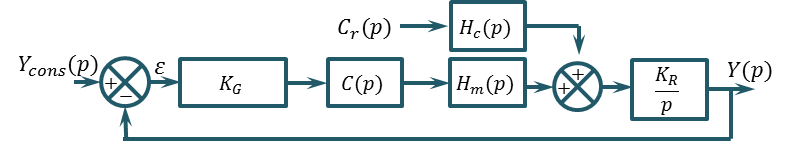
\includegraphics[width=\linewidth]{image10}
\end{center} 


Avec : 

\noindent $H_M (p)=\dfrac{K_M}{(1+T_E p)(1+T_M p)} \text{ et }
H_C (p)=\dfrac{\dfrac{\left(R+Lp\right)K_M}{K_C}}{(1+T_E p)(1+T_M p)}$.
%\item $C_R (p)=C_r/p$;
%\item $K_R=R_p \lambda$.
%\end{itemize}
\fi

\subparagraph{}
\textit{Donner l'expression de $\varepsilon(p)$.}
\ifprof
\begin{corrige}~\\
On raisonne par superposition :

Si $C_r (p)=0$: 

$$Y_1 (p)
=Y_{\text{cons}}(p) \dfrac{\dfrac{K_G K_{\text{Capt}} C(p) H_m (p) K_r}{p}}{1+\dfrac{K_G K_{\text{Capt}} C(p) H_m (p) K_r}{p}}$$

$$
=Y_{\text{cons}} (p) \dfrac{K_G K_{\text{Capt}} C(p) H_m (p) K_r}{p+K_G K_{\text{Capt}} C(p) H_m (p) K_r } 
$$

$$
=Y_{\text{cons}} (p) \dfrac{K_G K_{\text{Capt}} C(p) K_M  K_r}{(1+T_E p)(1+T_M p)p+K_G K_{\text{Capt}} C(p) K_M K_r )}$$.

\end{corrige}

\begin{corrige}
Si $Y_{\text{Cons}} (p)=0$ :

$$Y_2 (p)
=C_r (p) \dfrac{\dfrac{H_c (p) K_r}{p}}{1+\dfrac{K_r K_G K_{\text{Capt}} C(p) H_m (p)}{p} }$$

$$
=C_r (p) \dfrac{H_c (p) K_r}{p+K_r K_G K_{\text{Capt}} C(p) H_m (p) }$$
$$
=C_r (p) \dfrac{\dfrac{(R+Lp) K_M  K_r}{K_C }}{(1+T_E p)(1+T_M p)p+K_r K_G K_{\text{Capt}} C(p) K_M }$$

On a donc :
$Y(p)=Y_1 (p)+Y_2 (p)$.

\end{corrige}
\else
\fi

\subparagraph{}
\textit{On souhaite déterminer l'erreur en position du système. Calculer l'écart statique pour $C(p)=K_p$. Pouvait-on prévoir le résultat ?}
\ifprof
\begin{corrige}
\end{corrige}
\else
\fi


\subparagraph{}
\textit{On souhaite déterminer l'erreur en position du système. Calculer l'écart statique pour $C(p)=\dfrac{K_i}{p}$. Pouvait-on prévoir le résultat ?}
\ifprof
\begin{corrige}
\end{corrige}
\else
\fi


\subparagraph{}
\textit{On souhaite déterminer l'erreur en vitesse du système. Calculer l'erreur pour $C(p)=\dfrac{K_i}{p}$. Pouvait-on prévoir le résultat ?}
\ifprof
\begin{corrige}
\end{corrige}
\else
\fi


\subparagraph{}
\textit{On souhaite déterminer l'erreur pour un entrée en position du système avec une perturbation de type rampe. Calculer l'erreur pour $C(p)=\dfrac{K_i}{p}$. Pouvait-on prévoir le résultat ?}
\ifprof
\begin{corrige}
\end{corrige}
\else
\fi

%
%\subparagraph{}
%\textit{On souhaite que lorsque le système se déplace à vitesse constante, l'erreur sur la vitesse atteinte par le système soit nulle. Quelle sollicitation doit-on utiliser. Calculer l'écart statique pour $C(p)=K_p$ puis $C(p)=\dfrac{K_i}{p}$.}
%\ifprof
%\begin{corrige}
%\end{corrige}
%\else
%\fi
%
%\subparagraph{}
%\textit{Conclure.}
%\ifprof
%\begin{corrige}
%\end{corrige}
%\else
%\fi

%\ifprof
%\else
%
%Afin de répondre totalement au cahier des charges, l'utilisation d'un correcteur proportionnel intégral dérivé est retenue. En effet, la commande de l'axe intègre directement ce type de correcteur. Dans la suite du problème, le correcteur $C(p)$ sera de la forme : $C(p)=K_I \left(1+\dfrac{1}{(T_I p}\right)\left(1+T_D p\right)$. Le réglage des coefficients a été fait par simulation numérique.
%Afin de vérifier maintenant le critère de rapidité, on donne la réponse temporelle (figure page suivante) de l'axe à un échelon de position de $\SI{1}{m}$.
%
%\fi
%
%\subparagraph{}
%\textit{Conclure sur la conformité au cahier des charges du système ainsi réglé.}
%\ifprof
%\begin{corrige}
%\end{corrige}
%\else
%\fi
%
%\ifprof
%\else
% 
% \begin{center}
%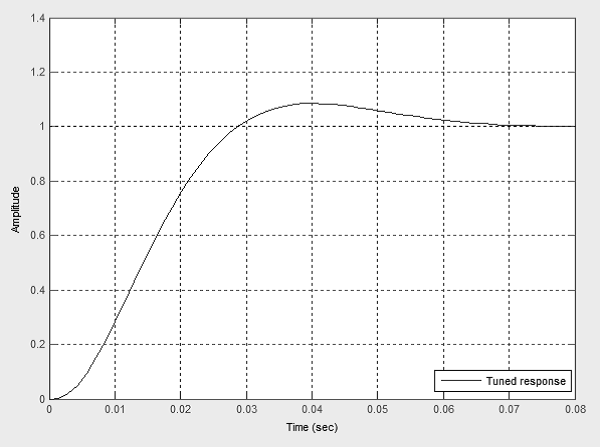
\includegraphics[width=7cm]{image11}
%\end{center} 
%
%\fi
% 
%
%\subparagraph{}
%\textit{Tracer de diagramme de Bode.}
%\ifprof
%\begin{corrige}
%\end{corrige}
%\else
%\fi
%
%\ifprof
%\else
%
%On considère $C_R (p)=0$. On prendra $K_M=\SI{0,8}{rad.s^{-1}.V^{-1}}$, $T_e=\SI{0,0051}{s}$,$T_m=\SI{0,0074}{s}$.
%\fi
%
%\subparagraph{}
%\textit{Tracer le diagramme de Bode de la fonction de transfert en boucle ouverte pour $C(p)=1$. Déterminer les marges de phase et les marges de gain.}
%\ifprof
%\begin{corrige}
%\end{corrige}
%\else
%\fi
% 
%\subparagraph{}
%\textit{Tracer le diagramme de Bode de la fonction de transfert en boucle ouverte pour $C(p)=\dfrac{1}{p}$. Déterminer les marges de phase et les marges de gain.}
%\ifprof
%\begin{corrige}
%\end{corrige}
%\else
%\fi
%
%\ifprof
%\else
%
%On donne ci-dessous les diagrammes de Bode avec les correcteurs optimisés. Déterminer les marges de gain et marges de phase. 
%\fi
%
%\section*{Vérification des performances de l'axe du magasin de rivets}
%\ifprof
%\else
%
%Afin de vérifier les réglages précédents, un essai sur le système réel est réalisé. Une consigne de \SI{2}{m} est donnée. L'absence de système d'acquisition dédié impose un système de mesure extérieur au système réel. C'est un dispositif d'analyse d'image qui est retenu pour ces mesures.
%\fi
%
%\subparagraph{}
%\textit{À partir des relevés ci-dessous, conclure sur le respect des exigences fonctionnelles de l'axe du magasin de stockage des rivets (Exigence 1.1).}
%\ifprof
%\begin{corrige}
%\end{corrige}
%\else
%\fi
 
\end{multicols}
%
%\ifprof
%\else
%
%\begin{center}
%\begin{tabular}{cc}
%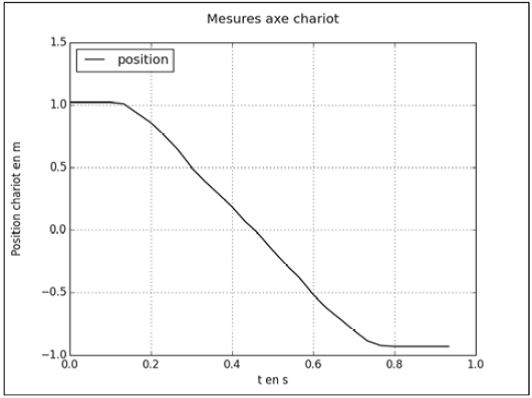
\includegraphics[width=7cm]{image13} &
%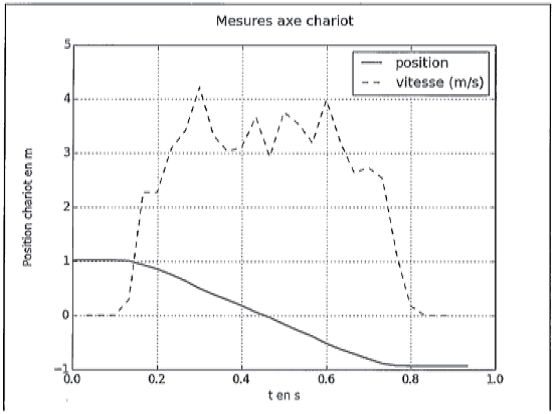
\includegraphics[width=7cm]{image14}
%
%\end{tabular}
%\end{center}
%
% \begin{center}
%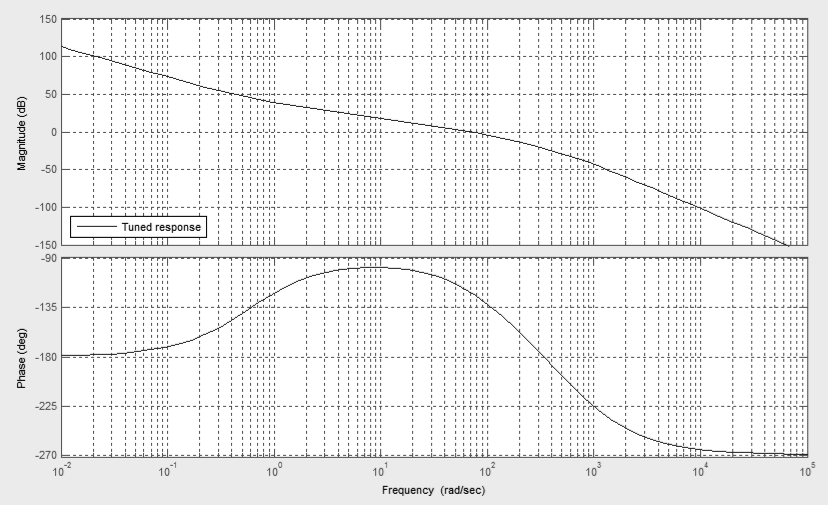
\includegraphics[width=\textwidth]{image12}
%\end{center} 
%\fi

%\end{document}


%% Application
%% Sujet
%\newpage
%\fichetrue \proffalse \tdtrue \coursfalse
%\graphicspath{{../style/png/}{../Chapitre_01_Stabilite/Application_01/images/}}
%%\documentclass[10pt,fleqn]{article} % Default font size and left-justified equations
%\usepackage[%
%    pdftitle={Modélisation SLCI : Stabilité des systèmes},
%    pdfauthor={Xavier Pessoles}]{hyperref}
%    
%%%%%%%%%%%%%%%%%%%%%%%%%%%%%%%%%%%%%%%%%%
% Original author:
% Mathias Legrand (legrand.mathias@gmail.com) with modifications by:
% Vel (vel@latextemplates.com)
% License:
% CC BY-NC-SA 3.0 (http://creativecommons.org/licenses/by-nc-sa/3.0/)
%%%%%%%%%%%%%%%%%%%%%%%%%%%%%%%%%%%%%%%%%

%----------------------------------------------------------------------------------------
%	VARIOUS REQUIRED PACKAGES AND CONFIGURATIONS
%----------------------------------------------------------------------------------------

%\usepackage[top=2.5cm,bottom=2cm,left=2cm,right=2cm,headsep=40pt,a4paper]{geometry} % Page margins
\usepackage[top=2cm,bottom=3cm,left=2cm,right=2cm,a4paper]{geometry} % Page margins

\usepackage{graphicx} % Required for including pictures

\usepackage{lipsum} % Inserts dummy text

\usepackage{tikz} % Required for drawing custom shapes

\usepackage[francais]{babel} % English language/hyphenation
\frenchbsetup{StandardLists=true} % Pour éviter la collision babel enumitem pour les listes

\usepackage{enumitem} % Customize lists
\setlist{nolistsep} % Reduce spacing between bullet points and numbered lists

\usepackage{booktabs} % Required for nicer horizontal rules in tables

\usepackage{xcolor} % Required for specifying colors by name
%\definecolor{ocre}{RGB}{243,102,25} % Define the orange color used for highlighting throughout the book
 \definecolor{ocre}{RGB}{49,133,156} % Couleur ''bleue''
\definecolor{violetf}{RGB}{112,48,160} % Couleur ''violet''
\usepackage{enumitem}
\usepackage{pifont} % Pour les dinglist
\usepackage{multicol}
\usepackage{array} % Centrage vertical dans les tableaux

%----------------------------------------------------------------------------------------
%	FONTS
%----------------------------------------------------------------------------------------

\usepackage{multicol}
\usepackage{siunitx}
\sisetup{output-decimal-marker = {,}}


\usepackage{avant} % Use the Avantgarde font for headings
%\usepackage{times} % Use the Times font for headings
%\usepackage{mathptmx} % Use the Adobe Times Roman as the default text font together with math symbols from the Sym­bol, Chancery and Com­puter Modern fonts
\usepackage[adobe-utopia]{mathdesign}
\usepackage{microtype} % Slightly tweak font spacing for aesthetics
\usepackage[utf8]{inputenc} % Required for including letters with accents
\usepackage[T1]{fontenc} % Use 8-bit encoding that has 256 glyphs

%----------------------------------------------------------------------------------------
%	BIBLIOGRAPHY AND INDEX
%----------------------------------------------------------------------------------------

%\usepackage[style=alphabetic,citestyle=numeric,sorting=nyt,sortcites=true,autopunct=true,babel=hyphen,hyperref=true,abbreviate=false,backref=true,backend=biber]{biblatex}
\usepackage[style=alphabetic,citestyle=numeric,sorting=nyt,sortcites=true,autopunct=true,hyperref=true,abbreviate=false,backref=true,backend=biber]{biblatex}
\addbibresource{bibliography.bib} % BibTeX bibliography file
\defbibheading{bibempty}{}

\usepackage{calc} % For simpler calculation - used for spacing the index letter headings correctly
\usepackage{makeidx} % Required to make an index
\makeindex % Tells LaTeX to create the files required for indexing

%----------------------------------------------------------------------------------------
%	MAIN TABLE OF CONTENTS
%----------------------------------------------------------------------------------------

\usepackage{titletoc} % Required for manipulating the table of contents

\setcounter{tocdepth}{2}     % Dans la table des matieres
\setcounter{secnumdepth}{2}

\contentsmargin{0cm} % Removes the default margin

% Part text styling
\titlecontents{part}[0cm]
{\addvspace{20pt}\centering\large\bfseries}
{}
{}
{}

% Chapter text styling
\titlecontents{chapter}[1.25cm] % Indentation
{\addvspace{12pt}\large\sffamily\bfseries} % Spacing and font options for chapters
{\color{ocre!60}\contentslabel[\Large\thecontentslabel]{1.25cm}\color{ocre}} % Chapter number
{\color{ocre}}  
{\color{ocre!60}\normalsize\;\titlerule*[.5pc]{.}\;\thecontentspage} % Page number

% Section text styling
\titlecontents{section}[1.25cm] % Indentation
{\addvspace{3pt}\sffamily\bfseries} % Spacing and font options for sections
{\color{ocre!60}\contentslabel[\thecontentslabel]{1.25cm} \color{ocre}} % Section number
{\color{ocre}}
{\hfill\color{ocre!60}\thecontentspage} % Page number
[]

% Subsection text styling
\titlecontents{subsection}[1.25cm] % Indentation
{\addvspace{1pt}\sffamily\small} % Spacing and font options for subsections
{\contentslabel[\thecontentslabel]{1.25cm}} % Subsection number
{}
{\ \titlerule*[.5pc]{.}\;\thecontentspage} % Page number
[]


% Subsection text styling
\titlecontents{subsubsection}[1.25cm] % Indentation
{\addvspace{1pt}\sffamily\small} % Spacing and font options for subsections
{\contentslabel[\thecontentslabel]{1.25cm}} % Subsection number
{}
{\ \titlerule*[.5pc]{.}\;\thecontentspage} % Page number
[]

% List of figures
\titlecontents{figure}[0em]
{\addvspace{-5pt}\sffamily}
{\thecontentslabel\hspace*{1em}}
{}
{\ \titlerule*[.5pc]{.}\;\thecontentspage}
[]

% List of tables
\titlecontents{table}[0em]
{\addvspace{-5pt}\sffamily}
{\thecontentslabel\hspace*{1em}}
{}
{\ \titlerule*[.5pc]{.}\;\thecontentspage}
[]

%----------------------------------------------------------------------------------------
%	MINI TABLE OF CONTENTS IN PART HEADS
%----------------------------------------------------------------------------------------

% Chapter text styling
\titlecontents{lchapter}[0em] % Indenting
{\addvspace{15pt}\large\sffamily\bfseries} % Spacing and font options for chapters
{\color{ocre}\contentslabel[\Large\thecontentslabel]{1.25cm}\color{ocre}} % Chapter number
{}  
{\color{ocre}\normalsize\sffamily\bfseries\;\titlerule*[.5pc]{.}\;\thecontentspage} % Page number

% Section text styling
\titlecontents{lsection}[0em] % Indenting
{\sffamily\small} % Spacing and font options for sections
{\contentslabel[\thecontentslabel]{1.25cm}} % Section number
{}
{}

% Subsection text styling
\titlecontents{lsubsection}[.5em] % Indentation
{\normalfont\footnotesize\sffamily} % Font settings
{}
{}
{}

%----------------------------------------------------------------------------------------
%	PAGE HEADERS
%----------------------------------------------------------------------------------------

\usepackage{fancyhdr} % Required for header and footer configuration



\pagestyle{fancy}
 \renewcommand{\headrulewidth}{0pt}
 \fancyhead{}
 
 % ENTETES de page
 \fancyhead[L]{%
 \noindent\begin{minipage}[c]{2.6cm}%
 
\includegraphics[width=2cm]{logo_lycee.png}%
 \end{minipage}}

\fancyhead[C]{\rule{8cm}{.5pt}}

 \fancyhead[R]{%
 \noindent\begin{minipage}[c]{3cm}
 \begin{flushright}
 \footnotesize{\textit{\textsf{\xxtete}}}%
 \end{flushright}
 \end{minipage}
}

 \fancyfoot{}
 % PIEDS de page
\fancyfoot[C]{\rule{12cm}{.5pt}}
\renewcommand{\footrulewidth}{0.2pt}
\fancyfoot[C]{\footnotesize{\bfseries \thepage}}
\fancyfoot[L]{ 
\begin{minipage}[c]{.4\linewidth}
\noindent\footnotesize{{\xxauteur}}
\end{minipage}}

\fancyfoot[R]{\footnotesize{\xxpied}
\ifthenelse{\isodd{\value{page}}}{
\begin{tikzpicture}[overlay]
\node[shape=rectangle, 
      rounded corners = .25 cm,
	  draw= ocre,
	  line width=2pt, 
	  fill = ocre!10,
	  minimum width  = 2.5cm,
	  minimum height = 3cm,] at (\xxposongletx,\xxposonglety) {};
\node at (\xxposonglettext,\xxposonglety) {\rotatebox{90}{\textbf{\large\color{ocre}{\xxonglet}}}};
%{};
\end{tikzpicture}}{}
}



%
%
%
% Removes the header from odd empty pages at the end of chapters
\makeatletter
%\renewcommand{\cleardoublepage}{
%\clearpage\ifodd\c@page\else
%\hbox{}
%\vspace*{\fill}
%\thispagestyle{empty}
%\newpage
%\fi}

%\fancypagestyle{plain}{%
%\fancyhf{} % vide l’en-tête et le pied~de~page.
%%\fancyfoot[C]{\bfseries \thepage} % numéro de la page en cours en gras
%% et centré en pied~de~page.
%\fancyfoot[R]{\footnotesize{\xxpied}}
%\fancyfoot[C]{\rule{12cm}{.5pt}}
%\renewcommand{\footrulewidth}{0.2pt}
%\fancyfoot[C]{\footnotesize{\bfseries \thepage}}
%\fancyfoot[L]{ 
%\begin{minipage}[c]{.4\linewidth}
%\noindent\footnotesize{{\xxauteur}}
%\end{minipage}}}

\fancypagestyle{plain}{%
\fancyhf{} % vide l’en-tête et le pied~de~page.
\fancyfoot[C]{\rule{12cm}{.5pt}}
\renewcommand{\footrulewidth}{0.2pt}
\fancyfoot[C]{\footnotesize{\bfseries \thepage}}
\fancyfoot[L]{ 
\begin{minipage}[c]{.4\linewidth}
\noindent\footnotesize{{\xxauteur}}
\end{minipage}}
\fancyfoot[R]{\footnotesize{\xxpied}}
}



%----------------------------------------------------------------------------------------
%	THEOREM STYLES
%----------------------------------------------------------------------------------------

% Conflit avec la police adobe
%\usepackage{amsmath,amsfonts,amssymb,amsthm} % For math equations, theorems, symbols, etc
\usepackage{amsmath,amsthm}

\newcommand{\intoo}[2]{\mathopen{]}#1\,;#2\mathclose{[}}
\newcommand{\ud}{\mathop{\mathrm{{}d}}\mathopen{}}
\newcommand{\intff}[2]{\mathopen{[}#1\,;#2\mathclose{]}}
%\newtheorem{notation}{Notation}[chapter]
\newtheorem{notation}{Notation}[section]

% Boxed/framed environments
\newtheoremstyle{ocrenumbox}% % Theorem style name
{0pt}% Space above
{0pt}% Space below
{\normalfont}% % Body font
{}% Indent amount
{\small\bf\sffamily\color{ocre}}% % Theorem head font
{\;}% Punctuation after theorem head
{0.25em}% Space after theorem head
{\small\sffamily\color{ocre}\thmname{#1}\nobreakspace\thmnumber%{\@ifnotempty{#1}{}\@upn{#2}}% Theorem text (e.g. Theorem 2.1)
\thmnote{\nobreakspace\the\thm@notefont\sffamily\bfseries\color{black}---\nobreakspace#3.}} % Optional theorem note
\renewcommand{\qedsymbol}{$\blacksquare$}% Optional qed square


% Boite pour les corriges
\newtheoremstyle{correctionbox}% % Theorem style name
{0pt}% Space above
{0pt}% Space below
{\normalfont}% % Body font
{}% Indent amount
{\small\bf\sffamily\color{violet}}% % Theorem head font
{\;}% Punctuation after theorem head
{0.25em}% Space after theorem head
{\small\sffamily\color{ocre}\thmname{#1}\nobreakspace\thmnumber%{\@ifnotempty{#1}{}\@upn{#2}}% Theorem text (e.g. Theorem 2.1)
\thmnote{\nobreakspace\the\thm@notefont\sffamily\bfseries\color{black}---\nobreakspace#3.}} % Optional theorem note
\renewcommand{\qedsymbol}{$\blacksquare$}% Optional qed square



\newtheoremstyle{blacknumex}% Theorem style name
{5pt}% Space above
{5pt}% Space below
{\normalfont}% Body font
{} % Indent amount
{\small\bf\sffamily}% Theorem head font
{\;}% Punctuation after theorem head
{0.25em}% Space after theorem head
{\small\sffamily{\tiny\ensuremath{\blacksquare}}\nobreakspace\thmname{#1}\nobreakspace\thmnumber%{\@ifnotempty{#1}{}\@upn{#2}}% Theorem text (e.g. Theorem 2.1)
\thmnote{\nobreakspace\the\thm@notefont\sffamily\bfseries---\nobreakspace#3.}}% Optional theorem note

\newtheoremstyle{blacknumbox} % Theorem style name
{0pt}% Space above
{0pt}% Space below
{\normalfont}% Body font
{}% Indent amount
{\small\bf\sffamily}% Theorem head font
{\;}% Punctuation after theorem head
{0.25em}% Space after theorem head
{\small\sffamily\thmname{#1}\nobreakspace 
\thmnote{\nobreakspace\the\thm@notefont\sffamily\bfseries---\nobreakspace#3.}}% Optional theorem note

% Non-boxed/non-framed environments
\newtheoremstyle{ocrenum}% % Theorem style name
{5pt}% Space above
{5pt}% Space below
{\normalfont}% % Body font
{}% Indent amount
{\small\bf\sffamily\color{ocre}}% % Theorem head font
{\;}% Punctuation after theorem head
{0.25em}% Space after theorem head
{\small\sffamily\color{ocre}\thmname{#1}\nobreakspace%\thmnumber{\@ifnotempty{#1}{}\@upn{#2}}% Theorem text (e.g. Theorem 2.1)
\thmnote{\nobreakspace\the\thm@notefont\sffamily\bfseries\color{black}---\nobreakspace#3.}} % Optional theorem note
\renewcommand{\qedsymbol}{$\blacksquare$}% Optional qed square
\makeatother

% Environnement pour les titres de parties
\newtheoremstyle{partiebox} 
{0pt}% Space above
{0pt}% Space below
{\normalfont}% Body font
{}% Indent amount
{\small\bf\sffamily}% Theorem head font
{\;}% Punctuation after theorem head
{0.25em}% Space after theorem head




% Defines the theorem text style for each type of theorem to one of the three styles above
\newcounter{dummy} 
\numberwithin{dummy}{section}
\theoremstyle{ocrenumbox}
%\newtheorem{theoremeT}[dummy]{Théorème}
\newtheorem{theoremeT}[dummy]{Théorème}
\newtheorem{resultatT}[dummy]{Résultat}
\newtheorem{savoirT}[dummy]{Savoir}
\newtheorem{methodeT}[dummy]{Méthode}
\newtheorem{objectifT}[dummy]{Objectif}
%\newtheorem{problem}{Problem}[chapter]
\newtheorem{problem}{Problem}[section]
%\newtheorem{exerciseT}{Exercise}[chapter]
\newtheorem{exerciseT}{Exercice}[section]

\theoremstyle{blacknumex}
%\newtheorem{exampleT}{Example}[chapter]
\newtheorem{exempleT}{Exemple}[section]
\newtheorem{termT}{Terminal\\}[section]
\newtheorem{pyT}{Python\\}[section]
\newtheorem{sciT}{Scilab\\}[section]
\newtheorem{pseudoT}{Pseudo Code\\}[section]
\newtheorem{sqlT}{SQL\\}[section]

\theoremstyle{blacknumbox}
%\newtheorem{vocabulary}{Vocabulary}[chapter]
\newtheorem{vocabulary}{Vocabulaire}[section]
%\newtheorem{definitionT}{Definition}[section]
\newtheorem{definitionT}{Définition}[section]
\newtheorem{rappelT}{Rappel}[section]
\newtheorem{demoT}{Démonstration}[section]
\newtheorem{corollaryT}[dummy]{Corollaire}
\newtheorem{hypoT}{Hypothèse(s)}

\theoremstyle{ocrenum}
\newtheorem{proposition}[dummy]{Proposition}

\theoremstyle{partiebox}
\newtheorem{titrepartieT}[]{}
\newtheorem{titrechapitreT}[]{}

\theoremstyle{correctionbox}
\newtheorem{correctionT}[dummy]{\color{violet}{Correction}}

%----------------------------------------------------------------------------------------
%	DEFINITION OF COLORED BOXES
%----------------------------------------------------------------------------------------

\RequirePackage[framemethod=tikz]{mdframed} % Required for creating the theorem, definition, exercise and corollary boxes

% Theorem box
\newmdenv[skipabove=7pt,
skipbelow=7pt,
backgroundcolor=ocre!10,
linecolor=ocre,
innerleftmargin=5pt,
innerrightmargin=5pt,
innertopmargin=5pt,
leftmargin=0cm,
rightmargin=0cm,
innerbottommargin=5pt]{tBox}


% Correction
\newmdenv[skipabove=7pt,
skipbelow=7pt,
backgroundcolor=violet!10,
linecolor=violet,
innerleftmargin=5pt,
innerrightmargin=5pt,
innertopmargin=5pt,
leftmargin=0cm,
rightmargin=0cm,
innerbottommargin=5pt]{coBox}


% Exercise box	  
\newmdenv[skipabove=7pt,
skipbelow=7pt,
rightline=false,
leftline=true,
topline=false,
bottomline=false,
backgroundcolor=ocre!10,
linecolor=ocre,
innerleftmargin=5pt,
innerrightmargin=5pt,
innertopmargin=5pt,
innerbottommargin=5pt,
leftmargin=0cm,
rightmargin=0cm,
linewidth=4pt]{eBox}	

% Definition box
\newmdenv[skipabove=7pt,
skipbelow=7pt,
rightline=false,
leftline=true,
topline=false,
bottomline=false,
backgroundcolor=ocre!10,
linecolor=ocre,
innerleftmargin=5pt,
innerrightmargin=5pt,
innertopmargin=0pt,
leftmargin=0cm,
rightmargin=0cm,
linewidth=4pt,
innerbottommargin=0pt]{dBox}	

% Demonstration box
\newmdenv[skipabove=7pt,
skipbelow=7pt,
rightline=false,
leftline=true,
topline=false,
bottomline=false,
%backgroundcolor=ocre!10,
linecolor=ocre,
innerleftmargin=5pt,
innerrightmargin=5pt,
innertopmargin=0pt,
leftmargin=0cm,
rightmargin=0cm,
linewidth=4pt,
innerbottommargin=0pt]{demoBox}	

% Corollary box
\newmdenv[skipabove=7pt,
skipbelow=7pt,
rightline=false,
leftline=true,
topline=false,
bottomline=false,
linecolor=gray,
backgroundcolor=black!5,
innerleftmargin=5pt,
innerrightmargin=5pt,
innertopmargin=5pt,
leftmargin=0cm,
rightmargin=0cm,
linewidth=4pt,
innerbottommargin=5pt]{cBox}


% Hypothèses
\newmdenv[skipabove=7pt,
skipbelow=7pt,
rightline=false,
leftline=true,
topline=false,
bottomline=false,
linecolor=gray,
backgroundcolor=black!5,
innerleftmargin=5pt,
innerrightmargin=5pt,
innertopmargin=5pt,
leftmargin=0cm,
rightmargin=0cm,
linewidth=4pt,
innerbottommargin=5pt]{hyBox}


% Boite pour le titre de la partie (pBox)
\newmdenv[skipabove=7pt,
skipbelow=7pt,
rightline=true,
leftline=false,
topline=false,
bottomline=false,
linecolor=ocre,
backgroundcolor=none,
innerleftmargin=5pt,
innerrightmargin=5pt,
innertopmargin=5pt,
leftmargin=0cm,
rightmargin=0cm,
linewidth=4pt,
innerbottommargin=5pt]{pBox}

% Boite pour le titre du chapitre (chBox)
\newmdenv[skipabove=7pt,
skipbelow=7pt,
rightline=false,
leftline=true,
topline=false,
bottomline=false,
linecolor=ocre,
%backgroundcolor=black!5,
innerleftmargin=5pt,
innerrightmargin=5pt,
innertopmargin=5pt,
leftmargin=0cm,
rightmargin=0cm,
linewidth=4pt,
innerbottommargin=5pt]{chBox}


% Boite pour les exemples
\newmdenv[skipabove=7pt,
skipbelow=7pt,
rightline=false,
leftline=true,
topline=false,
bottomline=false,
linecolor=gray,
backgroundcolor=white,
innerleftmargin=5pt,
innerrightmargin=5pt,
innertopmargin=5pt,
leftmargin=0cm,
rightmargin=0cm,
linewidth=4pt,
innerbottommargin=5pt]{exBox}

% Boite pour le terminal
\newmdenv[skipabove=7pt,
skipbelow=7pt,
rightline=false,
leftline=true,
topline=false,
bottomline=false,
linecolor=gray,
backgroundcolor=white,
innerleftmargin=5pt,
innerrightmargin=5pt,
innertopmargin=5pt,
leftmargin=0cm,
rightmargin=0cm,
linewidth=4pt,
innerbottommargin=5pt]{termBox}


% Boite pour Python
\newmdenv[skipabove=7pt,
skipbelow=7pt,
rightline=false,
leftline=true,
topline=false,
bottomline=false,
linecolor=gray,
backgroundcolor=white,
innerleftmargin=5pt,
innerrightmargin=5pt,
innertopmargin=0pt,
leftmargin=0cm,
rightmargin=0cm,
linewidth=4pt,
innerbottommargin=5pt]{pyBox}

% Boite pour scilab
\newmdenv[skipabove=7pt,
skipbelow=7pt,
rightline=false,
leftline=true,
topline=false,
bottomline=false,
linecolor=gray,
backgroundcolor=white,
innerleftmargin=5pt,
innerrightmargin=5pt,
innertopmargin=5pt,
leftmargin=0cm,
rightmargin=0cm,
linewidth=4pt,
innerbottommargin=5pt]{sciBox}


% Boite pour pseudo
\newmdenv[skipabove=7pt,
skipbelow=7pt,
rightline=false,
leftline=true,
topline=false,
bottomline=false,
linecolor=gray,
backgroundcolor=white,
innerleftmargin=5pt,
innerrightmargin=5pt,
innertopmargin=5pt,
leftmargin=0cm,
rightmargin=0cm,
linewidth=4pt,
innerbottommargin=5pt]{pseudoBox}

% Boite pour pseudo
\newmdenv[skipabove=7pt,
skipbelow=7pt,
rightline=false,
leftline=true,
topline=false,
bottomline=false,
linecolor=gray,
backgroundcolor=white,
innerleftmargin=5pt,
innerrightmargin=5pt,
innertopmargin=5pt,
leftmargin=0cm,
rightmargin=0cm,
linewidth=4pt,
innerbottommargin=5pt]{sqlBox}


% Creates an environment for each type of theorem and assigns it a theorem text style from the "Theorem Styles" section above and a colored box from above
\newenvironment{theorem}{\begin{tBox}\begin{theoremeT}}{\end{theoremeT}\end{tBox}}
\newenvironment{resultat}{\begin{tBox}\begin{resultatT}}{\end{resultatT}\end{tBox}}
\newenvironment{methode}{\begin{tBox}\begin{methodeT}}{\end{methodeT}\end{tBox}}
\newenvironment{savoir}{\begin{tBox}\begin{savoirT}}{\end{savoirT}\end{tBox}}
\newenvironment{obj}{\begin{tBox}\begin{objectifT}}{\end{objectifT}\end{tBox}}
\newenvironment{corrige}{\begin{coBox}\begin{correctionT}}{\end{correctionT}\end{coBox}}
\newenvironment{exercise}{\begin{eBox}\begin{exerciseT}}{\hfill{\color{ocre}\tiny\ensuremath{\blacksquare}}\end{exerciseT}\end{eBox}}				  
\newenvironment{exercice}{\begin{eBox}\begin{exerciseT}}{\hfill{\color{ocre}\tiny\ensuremath{\blacksquare}}\end{exerciseT}\end{eBox}}				  

\newenvironment{definition}{\begin{dBox}\begin{definitionT}}{\end{definitionT}\end{dBox}}	
\newenvironment{rappel}{\begin{dBox}\begin{rappelT}}{\end{rappelT}\end{dBox}}	
\newenvironment{defi}{\begin{dBox}\begin{definitionT}}{\end{definitionT}\end{dBox}}	
\newenvironment{demo}{\begin{demoBox}\begin{demoT}}{\end{demoT}\end{demoBox}}	
%\newenvironment{exemple}{\begin{exempleT}}{\hfill{\tiny\ensuremath{\blacksquare}}\end{exempleT}}		
\newenvironment{corollary}{\begin{cBox}\begin{corollaryT}}{\end{corollaryT}\end{cBox}}
\newenvironment{hypo}{\begin{hyBox}\begin{hypoT}}{\end{hypoT}\end{hyBox}}	\newenvironment{exemple}{\begin{exBox}\begin{exempleT}}{\hfill{\tiny\ensuremath{\blacksquare}}\end{exempleT}\end{exBox}}	
\newenvironment{titrepartie}{\begin{pBox}\begin{titrepartieT}}{\end{titrepartieT}\end{pBox}}	
\newenvironment{titrechapitre}{\begin{chBox}\begin{titrechapitreT}}{\end{titrechapitreT}\end{chBox}}	

\newenvironment{term}{ \begin{termBox}\begin{termT}}{\end{termT}\end{termBox}}
\newenvironment{py}{ \begin{pyBox}\begin{pyT}}{\end{pyT}\end{pyBox}}
\newenvironment{sci}{ \begin{sciBox}\begin{sciT}}{\end{sciT}\end{sciBox}}
\newenvironment{pseudo}{ \begin{pseudoBox}\begin{pseudoT}}{\end{pseudoT}\end{pseudoBox}}
\newenvironment{envsql}{ \begin{sqlBox}\begin{sqlT}}{\end{sqlT}\end{sqlBox}}


%----------------------------------------------------------------------------------------
%	REMARK ENVIRONMENT
%----------------------------------------------------------------------------------------

\newenvironment{remark}{\par\vspace{10pt}\small % Vertical white space above the remark and smaller font size
\begin{list}{}{
\leftmargin=35pt % Indentation on the left
\rightmargin=25pt}\item\ignorespaces % Indentation on the right
\makebox[-2.5pt]{\begin{tikzpicture}[overlay]
\node[draw=ocre!60,line width=1pt,circle,fill=ocre!25,font=\sffamily\bfseries,inner sep=2pt,outer sep=0pt] at (-15pt,0pt){\textcolor{ocre}{R}};\end{tikzpicture}} % Orange R in a circle
\advance\baselineskip -1pt}{\end{list}\vskip5pt} % Tighter line spacing and white space after remark

\newenvironment{rem}{\par\vspace{10pt}\small % Vertical white space above the remark and smaller font size
\begin{list}{}{
\leftmargin=35pt % Indentation on the left
\rightmargin=25pt}\item\ignorespaces % Indentation on the right
\makebox[-2.5pt]{\begin{tikzpicture}[overlay]
\node[draw=ocre!60,line width=1pt,circle,fill=ocre!25,font=\sffamily\bfseries,inner sep=2pt,outer sep=0pt] at (-15pt,0pt){\textcolor{ocre}{R}};\end{tikzpicture}} % Orange R in a circle
\advance\baselineskip -1pt}{\end{list}\vskip5pt} % Tighter line spacing and white space after remark


\newenvironment{warn}{\par\vspace{10pt}\small % Vertical white space above the remark and smaller font size
\begin{list}{}{
\leftmargin=35pt % Indentation on the left
\rightmargin=25pt}\item\ignorespaces % Indentation on the right
\makebox[-2.5pt]{\begin{tikzpicture}[overlay]
\node[draw=red!60,line width=1pt,circle,fill=red!25,font=\sffamily\bfseries,inner sep=2pt,outer sep=0pt] at (-15pt,0pt){\textcolor{black}{!}};\end{tikzpicture}} % Point d'exclamation dans un cercle
\advance\baselineskip -1pt}{\end{list}\vskip5pt} % Tighter line spacing and white space after remark


%----------------------------------------------------------------------------------------
%	SECTION NUMBERING IN THE MARGIN
%----------------------------------------------------------------------------------------
\setcounter{secnumdepth}{3}
\setcounter{tocdepth}{2}



\makeatletter
\renewcommand{\@seccntformat}[1]{\llap{\textcolor{ocre}{\csname the#1\endcsname}\hspace{1em}}}                    
\renewcommand{\section}{\@startsection{section}{1}{\z@}
{-4ex \@plus -1ex \@minus -.4ex}
{1ex \@plus.2ex }
{\normalfont\large\sffamily\bfseries}}
\renewcommand{\subsection}{\@startsection {subsection}{2}{\z@}
{-3ex \@plus -0.1ex \@minus -.4ex}
{0.5ex \@plus.2ex }
{\normalfont\sffamily\bfseries}}
\renewcommand{\subsubsection}{\@startsection {subsubsection}{3}{\z@}
{-2ex \@plus -0.1ex \@minus -.2ex}
{.2ex \@plus.2ex }
{\normalfont\small\sffamily\bfseries}}                        
\renewcommand\paragraph{\@startsection{paragraph}{4}{\z@}
{-2ex \@plus-.2ex \@minus .2ex}
{.1ex}
{\normalfont\small\sffamily\bfseries}}

%----------------------------------------------------------------------------------------
%	PART HEADINGS
%----------------------------------------------------------------------------------------


%----------------------------------------------------------------------------------------
%	CHAPTER HEADINGS
%----------------------------------------------------------------------------------------

% \newcommand{\thechapterimage}{}%
% \newcommand{\chapterimage}[1]{\renewcommand{\thechapterimage}{#1}}%
% \def\@makechapterhead#1{%
% {\parindent \z@ \raggedright \normalfont
% \ifnum \c@secnumdepth >\m@ne
% \if@mainmatter
% \begin{tikzpicture}[remember picture,overlay]
% \node at (current page.north west)
% {\begin{tikzpicture}[remember picture,overlay]
% \node[anchor=north west,inner sep=0pt] at (0,0) {\includegraphics[width=\paperwidth]{\thechapterimage}};
% \draw[anchor=west] (\Gm@lmargin,-9cm) node [line width=2pt,rounded corners=15pt,draw=ocre,fill=white,fill opacity=0.5,inner sep=15pt]{\strut\makebox[22cm]{}};
% \draw[anchor=west] (\Gm@lmargin+.3cm,-9cm) node {\huge\sffamily\bfseries\color{black}\thechapter. #1\strut};
% \end{tikzpicture}};
% \end{tikzpicture}
% \else
% \begin{tikzpicture}[remember picture,overlay]
% \node at (current page.north west)
% {\begin{tikzpicture}[remember picture,overlay]
% \node[anchor=north west,inner sep=0pt] at (0,0) {\includegraphics[width=\paperwidth]{\thechapterimage}};
% \draw[anchor=west] (\Gm@lmargin,-9cm) node [line width=2pt,rounded corners=15pt,draw=ocre,fill=white,fill opacity=0.5,inner sep=15pt]{\strut\makebox[22cm]{}};
% \draw[anchor=west] (\Gm@lmargin+.3cm,-9cm) node {\huge\sffamily\bfseries\color{black}#1\strut};
% \end{tikzpicture}};
% \end{tikzpicture}
% \fi\fi\par\vspace*{270\p@}}}

%-------------------------------------------

\def\@makeschapterhead#1{%
\begin{tikzpicture}[remember picture,overlay]
\node at (current page.north west)
{\begin{tikzpicture}[remember picture,overlay]
\node[anchor=north west,inner sep=0pt] at (0,0) {\includegraphics[width=\paperwidth]{\thechapterimage}};
\draw[anchor=west] (\Gm@lmargin,-9cm) node [line width=2pt,rounded corners=15pt,draw=ocre,fill=white,fill opacity=0.5,inner sep=15pt]{\strut\makebox[22cm]{}};
\draw[anchor=west] (\Gm@lmargin+.3cm,-9cm) node {\huge\sffamily\bfseries\color{black}#1\strut};
\end{tikzpicture}};
\end{tikzpicture}
\par\vspace*{270\p@}}
\makeatother

%----------------------------------------------------------------------------------------
%	HYPERLINKS IN THE DOCUMENTS
%----------------------------------------------------------------------------------------


\hypersetup{hidelinks,backref=true,pagebackref=true,hyperindex=true,colorlinks=false,breaklinks=true,urlcolor= ocre,bookmarks=true,bookmarksopen=false,pdftitle={Title},pdfauthor={Author}}
\usepackage{bookmark}
\bookmarksetup{
open,
numbered,
addtohook={%
\ifnum\bookmarkget{level}=0 % chapter
\bookmarksetup{bold}%
\fi
\ifnum\bookmarkget{level}=-1 % part
\bookmarksetup{color=ocre,bold}%
\fi
}
}

%----------------------------------------------------------------------------------------
%	
%----------------------------------------------------------------------------------------

\newcommand{\thechapterimage}{}%
\newcommand{\chapterimage}[1]{\renewcommand{\thechapterimage}{#1}}%
\def\@makechapterhead#1{%
{\parindent \z@ \raggedright \normalfont
\begin{tikzpicture}[remember picture,overlay]
\node at (current page.north west)
{\begin{tikzpicture}[remember picture,overlay]
\node[anchor=north west,inner sep=0pt] at (0,0) {\includegraphics[width=\paperwidth]{\thechapterimage}};
%\draw[anchor=west] (\Gm@lmargin,-9cm) node [line width=2pt,rounded corners=15pt,draw=ocre,fill=white,fill opacity=0.5,inner sep=15pt]{\strut\makebox[22cm]{}};
%\draw[anchor=west] (\Gm@lmargin+.3cm,-9cm) node {\huge\sffamily\bfseries\color{black}\thechapter. #1\strut};
\end{tikzpicture}};
\end{tikzpicture}
\par\vspace*{270\p@}
}}

 \newcounter{exo}


\makeatletter             
\renewcommand{\subparagraph}{\@startsection{exo}{5}{\z@}%
                                    {-2ex \@plus-.2ex \@minus .2ex}%
                                    {0ex}%               
{\normalfont\bfseries Question \hspace{.7cm} }}
\makeatother
\renewcommand{\thesubparagraph}{\arabic{subparagraph}} 
\makeatletter


\usepackage{textcomp}

% Définition des booleéns
\newif\iffiche
\newif\ifprof
\newif\iftd
\newif\ifcours
\newif\ifnormal
\newif\ifdifficile
\newif\iftdifficile
\newif\ifcolle
\newif\iflivret
%%%%%%%%%%%%%
% Définition des vecteurs 
%%%%%%%%%%%%
\newcommand{\vect}[1]{\overrightarrow{#1}}
\newcommand{\axe}[2]{\left(#1,\vect{#2}\right)}
\newcommand{\couple}[2]{\left(#1,\vect{#2}\right)}
\newcommand{\angl}[2]{\left(\vect{#1},\vect{#2}\right)}

\newcommand{\rep}[1]{\mathcal{R}_{#1}}
\newcommand{\quadruplet}[4]{\left(#1;#2,#3,#4 \right)}
\newcommand{\repere}[4]{\left(#1;\vect{#2},\vect{#3},\vect{#4} \right)}
\newcommand{\base}[3]{\left(\vect{#1},\vect{#2},\vect{#3} \right)}


\newcommand{\vx}[1]{\vect{x_{#1}}}
\newcommand{\vy}[1]{\vect{y_{#1}}}
\newcommand{\vz}[1]{\vect{z_{#1}}}

% d droit pour le calcul différentiel
\newcommand{\dd}{\text{d}}

\newcommand{\inertie}[2]{I_{#1}\left( #2\right)}
\newcommand{\matinertie}[7]{
\begin{pmatrix}
#1 & #6 & #5 \\
#6 & #2 & #4 \\
#5 & #4 & #3 \\
\end{pmatrix}_{#7}}
%%%%%%%%%%%%
% Définition des torseurs 
%%%%%%%%%%%%

\newcommand{\ec}[2]{%
\mathcal{E}_c\left(#1/#2\right)}

\newcommand{\pext}[3]{%
\mathcal{P}\left(#1\rightarrow#2/#3\right)}

\newcommand{\pint}[3]{%
\mathcal{P}\left(#1 \stackrel{\text{#3}}{\leftrightarrow} #2\right)}


 \newcommand{\torseur}[1]{%
\left\{{#1}\right\}
}

\newcommand{\torseurcin}[3]{%
\left\{\mathcal{#1} \left(#2/#3 \right) \right\}
}

\newcommand{\torseurci}[2]{%
\left\{\sigma \left(#1/#2 \right) \right\}
}
\newcommand{\torseurdyn}[2]{%
\left\{\mathcal{D} \left(#1/#2 \right) \right\}
}


\newcommand{\torseurstat}[3]{%
\left\{\mathcal{#1} \left(#2\rightarrow #3 \right) \right\}
}


 \newcommand{\torseurc}[8]{%
%\left\{#1 \right\}=
\left\{
{#1}
\right\}
 = 
\left\{%
\begin{array}{cc}%
{#2} & {#5}\\%
{#3} & {#6}\\%
{#4} & {#7}\\%
\end{array}%
\right\}_{#8}%
}

 \newcommand{\torseurcol}[7]{
\left\{%
\begin{array}{cc}%
{#1} & {#4}\\%
{#2} & {#5}\\%
{#3} & {#6}\\%
\end{array}%
\right\}_{#7}%
}

 \newcommand{\torseurl}[3]{%
%\left\{\mathcal{#1}\right\}_{#2}=%
\left\{%
\begin{array}{l}%
{#1} \\%
{#2} %
\end{array}%
\right\}_{#3}%
}

% Vecteur vitesse
 \newcommand{\vectv}[3]{%
\vect{V\left( {#1} \in {#2}/{#3}\right)}
}

% Vecteur force
\newcommand{\vectf}[2]{%
\vect{R\left( {#1} \rightarrow {#2}\right)}
}

% Vecteur moment stat
\newcommand{\vectm}[3]{%
\vect{\mathcal{M}\left( {#1}, {#2} \rightarrow {#3}\right)}
}




% Vecteur résultante cin
\newcommand{\vectrc}[2]{%
\vect{R_c \left( {#1}/ {#2}\right)}
}
% Vecteur moment cin
\newcommand{\vectmc}[3]{%
\vect{\sigma \left( {#1}, {#2} /{#3}\right)}
}


% Vecteur résultante dyn
\newcommand{\vectrd}[2]{%
\vect{R_d \left( {#1}/ {#2}\right)}
}
% Vecteur moment dyn
\newcommand{\vectmd}[3]{%
\vect{\delta \left( {#1}, {#2} /{#3}\right)}
}

% Vecteur accélération
 \newcommand{\vectg}[3]{%
\vect{\Gamma \left( {#1} \in {#2}/{#3}\right)}
}

% Vecteur omega
 \newcommand{\vecto}[2]{%
\vect{\Omega\left( {#1}/{#2}\right)}
}
% }$$\left\{\mathcal{#1} \right\}_{#2} =%
% \left\{%
% \begin{array}{c}%
%  #3 \\%
%  #4 %
% \end{array}%
% \right\}_{#5}}
%\usepackage{multicol}
%\usepackage{siunitx}
%\fichetrue
%%\fichefalse
%
%\proftrue
%\proffalse
%
%\tdtrue
%%\tdfalse
%
%\courstrue
%\coursfalse
%
%\def\discipline{Sciences \\Industrielles de \\ l'Ingénieur}
%\def\xxtete{Sciences Industrielles de l'Ingénieur}
%
%\def\classe{PSI$\star$ -- MP}
%\def\xxnumpartie{Cycle 02}
%\def\xxpartie{Modéliser les systèmes asservis dans le but de prévoir leur comportement}
%
%
%\def\xxnumchapitre{Chapitre 1 \vspace{.2cm}}
%\def\xxchapitre{\hspace{.12cm} Stabilité des systèmes}
%
%
%\def\xxtitreexo{Application}%Motorisation du moteur Haibike}
%\def\xxsourceexo{\hspace{.2cm}}% \footnotesize{Patrick Dupas, \url{http://patrick.dupas.chez-alice.fr/}.}}
%
%
%\def\xxposongletx{2}
%\def\xxposonglettext{1.45}
%\def\xxposonglety{20}
%%\def\xxonglet{Part. 1 -- Ch. 3}
%\def\xxonglet{Cycle 02}
%
%\def\xxactivite{Application}
%\def\xxauteur{\textsl{X. Pessoles}}
%
%\def\xxcompetences{%
%\textsl{%
%\textbf{Savoirs et compétences :}\\
%%Les sources sont associées par un \emph{hacheur série}. La détermination des grandeurs électriques associées à ce montage permet de conclure vis à vis du cahier des charges.
%%\noindent \textbf{Résoudre :} à partir des modèles retenus :
%%\begin{itemize}[label=\ding{112},font=\color{ocre}] 
%%\item choisir une méthode de résolution analytique, graphique, numérique;
%%\item mettre en \oe{}uvre une méthode de résolution.
%%\end{itemize}
%%\begin{itemize}[label=\ding{112},font=\color{ocre}] 
%%\item \textit{Rés -- C1.1 :} Loi entrée sortie géométrique et cinématique -- Fermeture géométrique.
%%\end{itemize}
%%
%%\noindent \textit{Mod2 -- C4.1 :} Représentation par schéma bloc.
%}}
%
%\def\xxfigures{
%%\includegraphics[width=.9\linewidth]{c-evolution}
%}%figues de la page de garde
%
%
%\def\xxpied{%
%Cycle 02 -- Modéliser les SLCI dans le but de prévoir leur comportement\\
%Chapitre 1 -- \xxactivite%
%}
%
%\setcounter{secnumdepth}{5}
%%---------------------------------------------------------------------------
%
%\usepackage{pgfplots}
%\begin{document}
%\def\pathfig{images}
%%\chapterimage{png/Fond_Cin}
%\pagestyle{empty}


%%%%%%%% PAGE DE GARDE COURS
\ifcours
\begin{tikzpicture}[remember picture,overlay]
\node at (current page.north west)
{\begin{tikzpicture}[remember picture,overlay]
\node[anchor=north west,inner sep=0pt] at (0,0) {\includegraphics[width=\paperwidth]{\thechapterimage}};
\draw[anchor=west] (-2cm,-8cm) node [line width=2pt,rounded corners=15pt,draw=ocre,fill=white,fill opacity=0.6,inner sep=40pt]{\strut\makebox[22cm]{}};
\draw[anchor=west] (1cm,-8cm) node {\huge\sffamily\bfseries\color{black} %
\begin{minipage}{1cm}
\rotatebox{90}{\LARGE\sffamily\textsc{\color{ocre}\textbf{\xxnumpartie}}}
\end{minipage} \hfill
\begin{minipage}[c]{14cm}
\begin{titrepartie}
\begin{flushright}
\renewcommand{\baselinestretch}{1.1} 
\Large\sffamily\textsc{\textbf{\xxpartie}}
\renewcommand{\baselinestretch}{1} 
\end{flushright}
\end{titrepartie}
\end{minipage} \hfill
\begin{minipage}[c]{3.5cm}
{\large\sffamily\textsc{\textbf{\color{ocre} \discipline}}}
\end{minipage} 
 };
\end{tikzpicture}};
\end{tikzpicture}


\begin{tikzpicture}[overlay]
\node[shape=rectangle, 
      rounded corners = .25 cm,
	  draw= ocre,
	  line width=2pt, 
	  fill = ocre!10,
	  minimum width  = 2.5cm,
	  minimum height = 3cm,] at (18cm,0) {};
\node at (17.7cm,0) {\rotatebox{90}{\textbf{\Large\color{ocre}{\classe}}}};
%{};
\end{tikzpicture}

\vspace{3.5cm}

\begin{tikzpicture}[remember picture,overlay]
\draw[anchor=west] (-2cm,-6cm) node {\huge\sffamily\bfseries\color{black} %
\begin{minipage}{2cm}
\begin{center}
\LARGE\sffamily\textsc{\color{ocre}\textbf{\xxactivite}}
\end{center}
\end{minipage} \hfill
\begin{minipage}[c]{15cm}
\begin{titrechapitre}
\renewcommand{\baselinestretch}{1.1} 
\Large\sffamily\textsc{\textbf{\xxnumchapitre}}

\Large\sffamily\textsc{\textbf{\xxchapitre}}
\vspace{.5cm}

\renewcommand{\baselinestretch}{1} 
\normalsize\normalfont
\xxcompetences
\end{titrechapitre}
\end{minipage}  };
\end{tikzpicture}
\vfill

\begin{flushright}
\begin{minipage}[c]{.3\linewidth}
\begin{center}
\xxfigures
\end{center}
\end{minipage}\hfill
\begin{minipage}[c]{.6\linewidth}
\startcontents
\printcontents{}{1}{}
\end{minipage}
\end{flushright}

\begin{tikzpicture}[remember picture,overlay]
\draw[anchor=west] (4.5cm,-.7cm) node {
\begin{minipage}[c]{.2\linewidth}
\begin{flushright}
\includegraphics[width=2cm]{logoCC}
\end{flushright}
\end{minipage}
\begin{minipage}[c]{.2\linewidth}
\textsl{\xxauteur} \\
\textsl{\classe}
\end{minipage}
 };
\end{tikzpicture}
\newpage
\pagestyle{fancy}

\newpage
\pagestyle{fancy}

\else
\fi


%%%%%%%% PAGE DE GARDE TD
\iftd
%\begin{tikzpicture}[remember picture,overlay]
%\node at (current page.north west)
%{\begin{tikzpicture}[remember picture,overlay]
%\draw[anchor=west] (-2cm,-3.25cm) node [line width=2pt,rounded corners=15pt,draw=ocre,fill=white,fill opacity=0.6,inner sep=40pt]{\strut\makebox[22cm]{}};
%\draw[anchor=west] (1cm,-3.25cm) node {\huge\sffamily\bfseries\color{black} %
%\begin{minipage}{1cm}
%\rotatebox{90}{\LARGE\sffamily\textsc{\color{ocre}\textbf{\xxnumpartie}}}
%\end{minipage} \hfill
%\begin{minipage}[c]{13.5cm}
%\begin{titrepartie}
%\begin{flushright}
%\renewcommand{\baselinestretch}{1.1} 
%\Large\sffamily\textsc{\textbf{\xxpartie}}
%\renewcommand{\baselinestretch}{1} 
%\end{flushright}
%\end{titrepartie}
%\end{minipage} \hfill
%\begin{minipage}[c]{3.5cm}
%{\large\sffamily\textsc{\textbf{\color{ocre} \discipline}}}
%\end{minipage} 
% };
%\end{tikzpicture}};
%\end{tikzpicture}

%%%%%%%%%% PAGE DE GARDE TD %%%%%%%%%%%%%%%
%\begin{tikzpicture}[overlay]
%\node[shape=rectangle, 
%      rounded corners = .25 cm,
%	  draw= ocre,
%	  line width=2pt, 
%	  fill = ocre!10,
%	  minimum width  = 2.5cm,
%	  minimum height = 2.5cm,] at (18.5cm,0) {};
%\node at (17.7cm,0) {\rotatebox{90}{\textbf{\Large\color{ocre}{\classe}}}};
%%{};
%\end{tikzpicture}

% PARTIE ET CHAPITRE
%\begin{tikzpicture}[remember picture,overlay]
%\draw[anchor=west] (-1cm,-2.1cm) node {\large\sffamily\bfseries\color{black} %
%\begin{minipage}[c]{15cm}
%\begin{flushleft}
%\xxnumchapitre \\
%\xxchapitre
%\end{flushleft}
%\end{minipage}  };
%\end{tikzpicture}

% Bandeau titre exo
\begin{tikzpicture}[remember picture,overlay]
\draw[anchor=west] (-2cm,-4cm) node {\huge\sffamily\bfseries\color{black} %
\begin{minipage}{5cm}
\begin{center}
\LARGE\sffamily\color{ocre}\textbf{\textsc{\xxactivite}}

\begin{center}
\xxfigures
\end{center}

\end{center}
\end{minipage} \hfill
\begin{minipage}[c]{12cm}
\begin{titrechapitre}
\renewcommand{\baselinestretch}{1.1} 
\large\sffamily\textbf{\textsc{\xxtitreexo}}

\small\sffamily{\textbf{\textit{\color{black!70}\xxsourceexo}}}
\vspace{.5cm}

\renewcommand{\baselinestretch}{1} 
\normalsize\normalfont
\xxcompetences
\end{titrechapitre}
\end{minipage}  };
\end{tikzpicture}

\else
\fi


%%%%%%%% PAGE DE GARDE FICHE
\iffiche
\begin{tikzpicture}[remember picture,overlay]
\node at (current page.north west)
{\begin{tikzpicture}[remember picture,overlay]
\draw[anchor=west] (-2cm,-3.25cm) node [line width=2pt,rounded corners=15pt,draw=ocre,fill=white,fill opacity=0.6,inner sep=40pt]{\strut\makebox[22cm]{}};
\draw[anchor=west] (1cm,-3.25cm) node {\huge\sffamily\bfseries\color{black} %
\begin{minipage}{1cm}
\rotatebox{90}{\LARGE\sffamily\textsc{\color{ocre}\textbf{\xxnumpartie}}}
\end{minipage} \hfill
\begin{minipage}[c]{14cm}
\begin{titrepartie}
\begin{flushright}
\renewcommand{\baselinestretch}{1.1} 
\large\sffamily\textsc{\textbf{\xxpartie} \\} 

\vspace{.2cm}

\normalsize\sffamily\textsc{\textbf{\xxnumchapitre -- \xxchapitre}}
\renewcommand{\baselinestretch}{1} 
\end{flushright}
\end{titrepartie}
\end{minipage} \hfill
\begin{minipage}[c]{3.5cm}
{\large\sffamily\textsc{\textbf{\color{ocre} \discipline}}}
\end{minipage} 
 };
\end{tikzpicture}};
\end{tikzpicture}


\begin{tikzpicture}[overlay]
\node[shape=rectangle, 
      rounded corners = .25 cm,
	  draw= ocre,
	  line width=2pt, 
	  fill = ocre!10,
	  minimum width  = 2.5cm,
	  minimum height = 2.5cm,] at (18.5cm,0.5cm) {};
%	  minimum height = 2.5cm,] at (18.5cm,0cm) {};
\node at (17.7cm,0.5) {\rotatebox{90}{\textsf{\textbf{\large\color{ocre}{\classe}}}}};
%{};
\end{tikzpicture}



\else
\fi



%\vspace{4.5cm}
%\pagestyle{fancy}
%\thispagestyle{plain}
%
%\def\columnseprulecolor{\color{ocre}}
%\setlength{\columnseprule}{0.4pt} 
%
%\def\pathfig{images}
%

%%%% Paramétrage du TD %%%%
\def\xxactivite{Application}
\def\xxauteur{\textsl{Xavier Pessoles}}


\def\xxnumchapitre{Chapitre 1 \vspace{.2cm}}
\def\xxchapitre{\hspace{.12cm} Stabilité des systèmes}

\def\xxcompetences{%
\textsl{%
\textbf{Savoirs et compétences :}\\
\vspace{-.4cm}
\begin{itemize}[label=\ding{112},font=\color{ocre}] 
%\item \textit{Mod3.C2 : } pôles dominants et réduction de l’ordre du modèle : principe, justification
%\item \textit{Res2.C4 : } stabilité des SLCI : définition entrée bornée -- sortie bornée (EB -- SB)	
%\item \textit{Res2.C5 : } stabilité des SLCI : équation caractéristique	
\item \textit{Res2.C6 : } stabilité des SLCI : position des pôles dans le plan complexe
\item \textit{Res2.C7 : } stabilité des SLCI : marges de stabilité (de gain et de phase)
\end{itemize}
}}


\def\xxfigures{
%\includegraphics[width=3cm]{SoloWheel_Orbit}\\
%\textit{}
}%figues de la page de garde

\def\xxtitreexo{Application}
\def\xxsourceexo{\hspace{.2cm} \footnotesize{Xavier Pessoles}}


\def\xxactivite{Application \ifprof  -- Corrigé \else \fi}
%\def\xxauteur{\textsl{P. Dupas.}}


\iflivret
\pagestyle{empty}


%%%%%%%% PAGE DE GARDE COURS
\ifcours
\begin{tikzpicture}[remember picture,overlay]
\node at (current page.north west)
{\begin{tikzpicture}[remember picture,overlay]
\node[anchor=north west,inner sep=0pt] at (0,0) {\includegraphics[width=\paperwidth]{\thechapterimage}};
\draw[anchor=west] (-2cm,-8cm) node [line width=2pt,rounded corners=15pt,draw=ocre,fill=white,fill opacity=0.6,inner sep=40pt]{\strut\makebox[22cm]{}};
\draw[anchor=west] (1cm,-8cm) node {\huge\sffamily\bfseries\color{black} %
\begin{minipage}{1cm}
\rotatebox{90}{\LARGE\sffamily\textsc{\color{ocre}\textbf{\xxnumpartie}}}
\end{minipage} \hfill
\begin{minipage}[c]{14cm}
\begin{titrepartie}
\begin{flushright}
\renewcommand{\baselinestretch}{1.1} 
\Large\sffamily\textsc{\textbf{\xxpartie}}
\renewcommand{\baselinestretch}{1} 
\end{flushright}
\end{titrepartie}
\end{minipage} \hfill
\begin{minipage}[c]{3.5cm}
{\large\sffamily\textsc{\textbf{\color{ocre} \discipline}}}
\end{minipage} 
 };
\end{tikzpicture}};
\end{tikzpicture}


\begin{tikzpicture}[overlay]
\node[shape=rectangle, 
      rounded corners = .25 cm,
	  draw= ocre,
	  line width=2pt, 
	  fill = ocre!10,
	  minimum width  = 2.5cm,
	  minimum height = 3cm,] at (18cm,0) {};
\node at (17.7cm,0) {\rotatebox{90}{\textbf{\Large\color{ocre}{\classe}}}};
%{};
\end{tikzpicture}

\vspace{3.5cm}

\begin{tikzpicture}[remember picture,overlay]
\draw[anchor=west] (-2cm,-6cm) node {\huge\sffamily\bfseries\color{black} %
\begin{minipage}{2cm}
\begin{center}
\LARGE\sffamily\textsc{\color{ocre}\textbf{\xxactivite}}
\end{center}
\end{minipage} \hfill
\begin{minipage}[c]{15cm}
\begin{titrechapitre}
\renewcommand{\baselinestretch}{1.1} 
\Large\sffamily\textsc{\textbf{\xxnumchapitre}}

\Large\sffamily\textsc{\textbf{\xxchapitre}}
\vspace{.5cm}

\renewcommand{\baselinestretch}{1} 
\normalsize\normalfont
\xxcompetences
\end{titrechapitre}
\end{minipage}  };
\end{tikzpicture}
\vfill

\begin{flushright}
\begin{minipage}[c]{.3\linewidth}
\begin{center}
\xxfigures
\end{center}
\end{minipage}\hfill
\begin{minipage}[c]{.6\linewidth}
\startcontents
\printcontents{}{1}{}
\end{minipage}
\end{flushright}

\begin{tikzpicture}[remember picture,overlay]
\draw[anchor=west] (4.5cm,-.7cm) node {
\begin{minipage}[c]{.2\linewidth}
\begin{flushright}
\includegraphics[width=2cm]{logoCC}
\end{flushright}
\end{minipage}
\begin{minipage}[c]{.2\linewidth}
\textsl{\xxauteur} \\
\textsl{\classe}
\end{minipage}
 };
\end{tikzpicture}
\newpage
\pagestyle{fancy}

\newpage
\pagestyle{fancy}

\else
\fi


%%%%%%%% PAGE DE GARDE TD
\iftd
%\begin{tikzpicture}[remember picture,overlay]
%\node at (current page.north west)
%{\begin{tikzpicture}[remember picture,overlay]
%\draw[anchor=west] (-2cm,-3.25cm) node [line width=2pt,rounded corners=15pt,draw=ocre,fill=white,fill opacity=0.6,inner sep=40pt]{\strut\makebox[22cm]{}};
%\draw[anchor=west] (1cm,-3.25cm) node {\huge\sffamily\bfseries\color{black} %
%\begin{minipage}{1cm}
%\rotatebox{90}{\LARGE\sffamily\textsc{\color{ocre}\textbf{\xxnumpartie}}}
%\end{minipage} \hfill
%\begin{minipage}[c]{13.5cm}
%\begin{titrepartie}
%\begin{flushright}
%\renewcommand{\baselinestretch}{1.1} 
%\Large\sffamily\textsc{\textbf{\xxpartie}}
%\renewcommand{\baselinestretch}{1} 
%\end{flushright}
%\end{titrepartie}
%\end{minipage} \hfill
%\begin{minipage}[c]{3.5cm}
%{\large\sffamily\textsc{\textbf{\color{ocre} \discipline}}}
%\end{minipage} 
% };
%\end{tikzpicture}};
%\end{tikzpicture}

%%%%%%%%%% PAGE DE GARDE TD %%%%%%%%%%%%%%%
%\begin{tikzpicture}[overlay]
%\node[shape=rectangle, 
%      rounded corners = .25 cm,
%	  draw= ocre,
%	  line width=2pt, 
%	  fill = ocre!10,
%	  minimum width  = 2.5cm,
%	  minimum height = 2.5cm,] at (18.5cm,0) {};
%\node at (17.7cm,0) {\rotatebox{90}{\textbf{\Large\color{ocre}{\classe}}}};
%%{};
%\end{tikzpicture}

% PARTIE ET CHAPITRE
%\begin{tikzpicture}[remember picture,overlay]
%\draw[anchor=west] (-1cm,-2.1cm) node {\large\sffamily\bfseries\color{black} %
%\begin{minipage}[c]{15cm}
%\begin{flushleft}
%\xxnumchapitre \\
%\xxchapitre
%\end{flushleft}
%\end{minipage}  };
%\end{tikzpicture}

% Bandeau titre exo
\begin{tikzpicture}[remember picture,overlay]
\draw[anchor=west] (-2cm,-4cm) node {\huge\sffamily\bfseries\color{black} %
\begin{minipage}{5cm}
\begin{center}
\LARGE\sffamily\color{ocre}\textbf{\textsc{\xxactivite}}

\begin{center}
\xxfigures
\end{center}

\end{center}
\end{minipage} \hfill
\begin{minipage}[c]{12cm}
\begin{titrechapitre}
\renewcommand{\baselinestretch}{1.1} 
\large\sffamily\textbf{\textsc{\xxtitreexo}}

\small\sffamily{\textbf{\textit{\color{black!70}\xxsourceexo}}}
\vspace{.5cm}

\renewcommand{\baselinestretch}{1} 
\normalsize\normalfont
\xxcompetences
\end{titrechapitre}
\end{minipage}  };
\end{tikzpicture}

\else
\fi


%%%%%%%% PAGE DE GARDE FICHE
\iffiche
\begin{tikzpicture}[remember picture,overlay]
\node at (current page.north west)
{\begin{tikzpicture}[remember picture,overlay]
\draw[anchor=west] (-2cm,-3.25cm) node [line width=2pt,rounded corners=15pt,draw=ocre,fill=white,fill opacity=0.6,inner sep=40pt]{\strut\makebox[22cm]{}};
\draw[anchor=west] (1cm,-3.25cm) node {\huge\sffamily\bfseries\color{black} %
\begin{minipage}{1cm}
\rotatebox{90}{\LARGE\sffamily\textsc{\color{ocre}\textbf{\xxnumpartie}}}
\end{minipage} \hfill
\begin{minipage}[c]{14cm}
\begin{titrepartie}
\begin{flushright}
\renewcommand{\baselinestretch}{1.1} 
\large\sffamily\textsc{\textbf{\xxpartie} \\} 

\vspace{.2cm}

\normalsize\sffamily\textsc{\textbf{\xxnumchapitre -- \xxchapitre}}
\renewcommand{\baselinestretch}{1} 
\end{flushright}
\end{titrepartie}
\end{minipage} \hfill
\begin{minipage}[c]{3.5cm}
{\large\sffamily\textsc{\textbf{\color{ocre} \discipline}}}
\end{minipage} 
 };
\end{tikzpicture}};
\end{tikzpicture}


\begin{tikzpicture}[overlay]
\node[shape=rectangle, 
      rounded corners = .25 cm,
	  draw= ocre,
	  line width=2pt, 
	  fill = ocre!10,
	  minimum width  = 2.5cm,
	  minimum height = 2.5cm,] at (18.5cm,0.5cm) {};
%	  minimum height = 2.5cm,] at (18.5cm,0cm) {};
\node at (17.7cm,0.5) {\rotatebox{90}{\textsf{\textbf{\large\color{ocre}{\classe}}}}};
%{};
\end{tikzpicture}



\else
\fi



\else
\pagestyle{empty}


%%%%%%%% PAGE DE GARDE COURS
\ifcours
\begin{tikzpicture}[remember picture,overlay]
\node at (current page.north west)
{\begin{tikzpicture}[remember picture,overlay]
\node[anchor=north west,inner sep=0pt] at (0,0) {\includegraphics[width=\paperwidth]{\thechapterimage}};
\draw[anchor=west] (-2cm,-8cm) node [line width=2pt,rounded corners=15pt,draw=ocre,fill=white,fill opacity=0.6,inner sep=40pt]{\strut\makebox[22cm]{}};
\draw[anchor=west] (1cm,-8cm) node {\huge\sffamily\bfseries\color{black} %
\begin{minipage}{1cm}
\rotatebox{90}{\LARGE\sffamily\textsc{\color{ocre}\textbf{\xxnumpartie}}}
\end{minipage} \hfill
\begin{minipage}[c]{14cm}
\begin{titrepartie}
\begin{flushright}
\renewcommand{\baselinestretch}{1.1} 
\Large\sffamily\textsc{\textbf{\xxpartie}}
\renewcommand{\baselinestretch}{1} 
\end{flushright}
\end{titrepartie}
\end{minipage} \hfill
\begin{minipage}[c]{3.5cm}
{\large\sffamily\textsc{\textbf{\color{ocre} \discipline}}}
\end{minipage} 
 };
\end{tikzpicture}};
\end{tikzpicture}


\begin{tikzpicture}[overlay]
\node[shape=rectangle, 
      rounded corners = .25 cm,
	  draw= ocre,
	  line width=2pt, 
	  fill = ocre!10,
	  minimum width  = 2.5cm,
	  minimum height = 3cm,] at (18cm,0) {};
\node at (17.7cm,0) {\rotatebox{90}{\textbf{\Large\color{ocre}{\classe}}}};
%{};
\end{tikzpicture}

\vspace{3.5cm}

\begin{tikzpicture}[remember picture,overlay]
\draw[anchor=west] (-2cm,-6cm) node {\huge\sffamily\bfseries\color{black} %
\begin{minipage}{2cm}
\begin{center}
\LARGE\sffamily\textsc{\color{ocre}\textbf{\xxactivite}}
\end{center}
\end{minipage} \hfill
\begin{minipage}[c]{15cm}
\begin{titrechapitre}
\renewcommand{\baselinestretch}{1.1} 
\Large\sffamily\textsc{\textbf{\xxnumchapitre}}

\Large\sffamily\textsc{\textbf{\xxchapitre}}
\vspace{.5cm}

\renewcommand{\baselinestretch}{1} 
\normalsize\normalfont
\xxcompetences
\end{titrechapitre}
\end{minipage}  };
\end{tikzpicture}
\vfill

\begin{flushright}
\begin{minipage}[c]{.3\linewidth}
\begin{center}
\xxfigures
\end{center}
\end{minipage}\hfill
\begin{minipage}[c]{.6\linewidth}
\startcontents
\printcontents{}{1}{}
\end{minipage}
\end{flushright}

\begin{tikzpicture}[remember picture,overlay]
\draw[anchor=west] (4.5cm,-.7cm) node {
\begin{minipage}[c]{.2\linewidth}
\begin{flushright}
\includegraphics[width=2cm]{logoCC}
\end{flushright}
\end{minipage}
\begin{minipage}[c]{.2\linewidth}
\textsl{\xxauteur} \\
\textsl{\classe}
\end{minipage}
 };
\end{tikzpicture}
\newpage
\pagestyle{fancy}

\newpage
\pagestyle{fancy}

\else
\fi


%%%%%%%% PAGE DE GARDE TD
\iftd
%\begin{tikzpicture}[remember picture,overlay]
%\node at (current page.north west)
%{\begin{tikzpicture}[remember picture,overlay]
%\draw[anchor=west] (-2cm,-3.25cm) node [line width=2pt,rounded corners=15pt,draw=ocre,fill=white,fill opacity=0.6,inner sep=40pt]{\strut\makebox[22cm]{}};
%\draw[anchor=west] (1cm,-3.25cm) node {\huge\sffamily\bfseries\color{black} %
%\begin{minipage}{1cm}
%\rotatebox{90}{\LARGE\sffamily\textsc{\color{ocre}\textbf{\xxnumpartie}}}
%\end{minipage} \hfill
%\begin{minipage}[c]{13.5cm}
%\begin{titrepartie}
%\begin{flushright}
%\renewcommand{\baselinestretch}{1.1} 
%\Large\sffamily\textsc{\textbf{\xxpartie}}
%\renewcommand{\baselinestretch}{1} 
%\end{flushright}
%\end{titrepartie}
%\end{minipage} \hfill
%\begin{minipage}[c]{3.5cm}
%{\large\sffamily\textsc{\textbf{\color{ocre} \discipline}}}
%\end{minipage} 
% };
%\end{tikzpicture}};
%\end{tikzpicture}

%%%%%%%%%% PAGE DE GARDE TD %%%%%%%%%%%%%%%
%\begin{tikzpicture}[overlay]
%\node[shape=rectangle, 
%      rounded corners = .25 cm,
%	  draw= ocre,
%	  line width=2pt, 
%	  fill = ocre!10,
%	  minimum width  = 2.5cm,
%	  minimum height = 2.5cm,] at (18.5cm,0) {};
%\node at (17.7cm,0) {\rotatebox{90}{\textbf{\Large\color{ocre}{\classe}}}};
%%{};
%\end{tikzpicture}

% PARTIE ET CHAPITRE
%\begin{tikzpicture}[remember picture,overlay]
%\draw[anchor=west] (-1cm,-2.1cm) node {\large\sffamily\bfseries\color{black} %
%\begin{minipage}[c]{15cm}
%\begin{flushleft}
%\xxnumchapitre \\
%\xxchapitre
%\end{flushleft}
%\end{minipage}  };
%\end{tikzpicture}

% Bandeau titre exo
\begin{tikzpicture}[remember picture,overlay]
\draw[anchor=west] (-2cm,-4cm) node {\huge\sffamily\bfseries\color{black} %
\begin{minipage}{5cm}
\begin{center}
\LARGE\sffamily\color{ocre}\textbf{\textsc{\xxactivite}}

\begin{center}
\xxfigures
\end{center}

\end{center}
\end{minipage} \hfill
\begin{minipage}[c]{12cm}
\begin{titrechapitre}
\renewcommand{\baselinestretch}{1.1} 
\large\sffamily\textbf{\textsc{\xxtitreexo}}

\small\sffamily{\textbf{\textit{\color{black!70}\xxsourceexo}}}
\vspace{.5cm}

\renewcommand{\baselinestretch}{1} 
\normalsize\normalfont
\xxcompetences
\end{titrechapitre}
\end{minipage}  };
\end{tikzpicture}

\else
\fi


%%%%%%%% PAGE DE GARDE FICHE
\iffiche
\begin{tikzpicture}[remember picture,overlay]
\node at (current page.north west)
{\begin{tikzpicture}[remember picture,overlay]
\draw[anchor=west] (-2cm,-3.25cm) node [line width=2pt,rounded corners=15pt,draw=ocre,fill=white,fill opacity=0.6,inner sep=40pt]{\strut\makebox[22cm]{}};
\draw[anchor=west] (1cm,-3.25cm) node {\huge\sffamily\bfseries\color{black} %
\begin{minipage}{1cm}
\rotatebox{90}{\LARGE\sffamily\textsc{\color{ocre}\textbf{\xxnumpartie}}}
\end{minipage} \hfill
\begin{minipage}[c]{14cm}
\begin{titrepartie}
\begin{flushright}
\renewcommand{\baselinestretch}{1.1} 
\large\sffamily\textsc{\textbf{\xxpartie} \\} 

\vspace{.2cm}

\normalsize\sffamily\textsc{\textbf{\xxnumchapitre -- \xxchapitre}}
\renewcommand{\baselinestretch}{1} 
\end{flushright}
\end{titrepartie}
\end{minipage} \hfill
\begin{minipage}[c]{3.5cm}
{\large\sffamily\textsc{\textbf{\color{ocre} \discipline}}}
\end{minipage} 
 };
\end{tikzpicture}};
\end{tikzpicture}


\begin{tikzpicture}[overlay]
\node[shape=rectangle, 
      rounded corners = .25 cm,
	  draw= ocre,
	  line width=2pt, 
	  fill = ocre!10,
	  minimum width  = 2.5cm,
	  minimum height = 2.5cm,] at (18.5cm,0.5cm) {};
%	  minimum height = 2.5cm,] at (18.5cm,0cm) {};
\node at (17.7cm,0.5) {\rotatebox{90}{\textsf{\textbf{\large\color{ocre}{\classe}}}}};
%{};
\end{tikzpicture}



\else
\fi



\fi
\setlength{\columnseprule}{.1pt}

\pagestyle{fancy}
\thispagestyle{plain}


\vspace{4.5cm}

\def\columnseprulecolor{\color{ocre}}
\setlength{\columnseprule}{0.4pt} 

%%%%%%%%%%%%%%%%%%%%%%%





\ifprof
\else
\begin{multicols}{2}
\fi

%\subsection*{Exercice 1 -- Réponse impulsionnelle (entrée Dirac)}
\setcounter{exo}{0}
On considère le schéma-blocs suivant. 
\begin{center}
\includegraphics[width=\linewidth]{fig_01}
\end{center}

On donne ci-dessous la réponse indicielle pour $K_C=1$.

\begin{center}
\includegraphics[width=\linewidth]{fig_02}
\end{center}


\subparagraph{}\textit{Justifier l'allure du diagramme du diagramme de Bode donné ci-dessous pour $K_C=1$.}

\subparagraph{}\textit{Donner graphiquement les marges de phase et de gain pour $K_C=1$.}
\ifprof
\begin{center}
\includegraphics[width=\linewidth]{cor_01}
\end{center}

\else
\fi


\subparagraph{}\textit{Donner analytiquement les marges de phase et de gain pour $K_C=1$ (méthode).}
\ifprof
\begin{corrige}
\textbf{Calcul de la marge de gain}
\begin{itemize}
\item On détermine $\omega_{180}$ tel que $\arg\left(\text{FTBO}(j\omega_{180})\right)=-180\degres$. 

$\arg\left(\text{FTBO}(j\omega)\right) $ $= -\arg\left( j\omega\right)-\arg\left( 1+ 10 j\omega\right)-\arg\left(1+0,5j\omega \right) $ $= - 90 - \arctan \left( 10 \omega \right) - \arctan \left( 0,5 \omega \right)$.

$\arg\left(\text{FTBO}(j\omega_{180})\right)=-180\degres$ 
$\Leftrightarrow - 90 - \arctan \left( 10 \omega \right) - \arctan \left( 0,5 \omega \right) = -180$

\begin{python}
import math as m
from pylab import *
from scipy.optimize import bisect 

def f(x):                                       
    res = m.pi/2 - m.atan(10*x) - m.atan(0.5*x)
    return res

zero1 = bisect(f, .1, 10)
\end{python}
On a $\omega=\SI{0,447}{rad.s^{-1}}$.
%$\Leftrightarrow - \arctan \left( 10 \omega \right) - \arctan \left( 0,5 \omega \right) = -90$
\end{itemize}

\end{corrige}
\else
\fi

\subparagraph{}\textit{Le cahier des charges impose des marges de gain et de phase minimales de \SI{12}{dB} et 40\degres. Déterminer
la plus grande valeur de $K_C$ permettant de vérifier ce cahier des charges}


\ifprof
\else
\end{multicols}
\fi



\ifprof
\else

\begin{center}
\includegraphics[width=\linewidth]{fig_03}
\end{center}

\fi


\ifprof
\begin{center}
\includegraphics[width=\linewidth]{cor_02}
\end{center}

\else
\fi


%\ifprof
%\else
%\noindent\begin{minipage}[c]{.4\linewidth}
%\begin{center}
%\includegraphics[width=\linewidth]{fig_03}
%\end{center}
%\end{minipage}\hfill
%\begin{minipage}[c]{.46\linewidth}
%\begin{center}
%\includegraphics[width=.9\linewidth]{fig_01}
%\end{center}
%\end{minipage}

\ifprof
\else
\begin{center}
\includegraphics[width=\linewidth]{img_04}
\end{center}
\fi

%
%\begin{center}
%\includegraphics[width=\linewidth]{fig_02}
%\end{center}
%
%\begin{center}
%\includegraphics[width=\linewidth]{fig_03}
%\end{center}
%
%\begin{center}
%\includegraphics[width=.8\linewidth]{fig_04}
%\end{center}


%
%\end{document}
%
%\subsection*{Exercice 3 -- Applications du critère du Revers}
%
%\subparagraph*{}\textit{On donne ci-dessous les lieux de transferts de plusieurs FTBO. Déterminer, à l'aide du critère du Revers si les systèmes sont stables en BF.}
%\subparagraph*{}\textit{Pour les systèmes stables déterminer les marges de gain et de phase.}
%
%\end{multicols}
%
%\begin{center}
%\includegraphics[width=\linewidth]{fig_02}
%\end{center}
%
%\begin{center}
%\includegraphics[width=\linewidth]{fig_03}
%\end{center}
%
%\begin{center}
%\includegraphics[width=.8\linewidth]{fig_04}
%\end{center}




%
%%% PAS DE CORRIGE !!!
%\newpage
%\fichetrue \proftrue \tdtrue \coursfalse
%\graphicspath{{../style/png/}{../Chapitre_01_Stabilite/Application_01/images/}}
%%\documentclass[10pt,fleqn]{article} % Default font size and left-justified equations
%\usepackage[%
%    pdftitle={Modélisation SLCI : Stabilité des systèmes},
%    pdfauthor={Xavier Pessoles}]{hyperref}
%    
%%%%%%%%%%%%%%%%%%%%%%%%%%%%%%%%%%%%%%%%%%
% Original author:
% Mathias Legrand (legrand.mathias@gmail.com) with modifications by:
% Vel (vel@latextemplates.com)
% License:
% CC BY-NC-SA 3.0 (http://creativecommons.org/licenses/by-nc-sa/3.0/)
%%%%%%%%%%%%%%%%%%%%%%%%%%%%%%%%%%%%%%%%%

%----------------------------------------------------------------------------------------
%	VARIOUS REQUIRED PACKAGES AND CONFIGURATIONS
%----------------------------------------------------------------------------------------

%\usepackage[top=2.5cm,bottom=2cm,left=2cm,right=2cm,headsep=40pt,a4paper]{geometry} % Page margins
\usepackage[top=2cm,bottom=3cm,left=2cm,right=2cm,a4paper]{geometry} % Page margins

\usepackage{graphicx} % Required for including pictures

\usepackage{lipsum} % Inserts dummy text

\usepackage{tikz} % Required for drawing custom shapes

\usepackage[francais]{babel} % English language/hyphenation
\frenchbsetup{StandardLists=true} % Pour éviter la collision babel enumitem pour les listes

\usepackage{enumitem} % Customize lists
\setlist{nolistsep} % Reduce spacing between bullet points and numbered lists

\usepackage{booktabs} % Required for nicer horizontal rules in tables

\usepackage{xcolor} % Required for specifying colors by name
%\definecolor{ocre}{RGB}{243,102,25} % Define the orange color used for highlighting throughout the book
 \definecolor{ocre}{RGB}{49,133,156} % Couleur ''bleue''
\definecolor{violetf}{RGB}{112,48,160} % Couleur ''violet''
\usepackage{enumitem}
\usepackage{pifont} % Pour les dinglist
\usepackage{multicol}
\usepackage{array} % Centrage vertical dans les tableaux

%----------------------------------------------------------------------------------------
%	FONTS
%----------------------------------------------------------------------------------------

\usepackage{multicol}
\usepackage{siunitx}
\sisetup{output-decimal-marker = {,}}


\usepackage{avant} % Use the Avantgarde font for headings
%\usepackage{times} % Use the Times font for headings
%\usepackage{mathptmx} % Use the Adobe Times Roman as the default text font together with math symbols from the Sym­bol, Chancery and Com­puter Modern fonts
\usepackage[adobe-utopia]{mathdesign}
\usepackage{microtype} % Slightly tweak font spacing for aesthetics
\usepackage[utf8]{inputenc} % Required for including letters with accents
\usepackage[T1]{fontenc} % Use 8-bit encoding that has 256 glyphs

%----------------------------------------------------------------------------------------
%	BIBLIOGRAPHY AND INDEX
%----------------------------------------------------------------------------------------

%\usepackage[style=alphabetic,citestyle=numeric,sorting=nyt,sortcites=true,autopunct=true,babel=hyphen,hyperref=true,abbreviate=false,backref=true,backend=biber]{biblatex}
\usepackage[style=alphabetic,citestyle=numeric,sorting=nyt,sortcites=true,autopunct=true,hyperref=true,abbreviate=false,backref=true,backend=biber]{biblatex}
\addbibresource{bibliography.bib} % BibTeX bibliography file
\defbibheading{bibempty}{}

\usepackage{calc} % For simpler calculation - used for spacing the index letter headings correctly
\usepackage{makeidx} % Required to make an index
\makeindex % Tells LaTeX to create the files required for indexing

%----------------------------------------------------------------------------------------
%	MAIN TABLE OF CONTENTS
%----------------------------------------------------------------------------------------

\usepackage{titletoc} % Required for manipulating the table of contents

\setcounter{tocdepth}{2}     % Dans la table des matieres
\setcounter{secnumdepth}{2}

\contentsmargin{0cm} % Removes the default margin

% Part text styling
\titlecontents{part}[0cm]
{\addvspace{20pt}\centering\large\bfseries}
{}
{}
{}

% Chapter text styling
\titlecontents{chapter}[1.25cm] % Indentation
{\addvspace{12pt}\large\sffamily\bfseries} % Spacing and font options for chapters
{\color{ocre!60}\contentslabel[\Large\thecontentslabel]{1.25cm}\color{ocre}} % Chapter number
{\color{ocre}}  
{\color{ocre!60}\normalsize\;\titlerule*[.5pc]{.}\;\thecontentspage} % Page number

% Section text styling
\titlecontents{section}[1.25cm] % Indentation
{\addvspace{3pt}\sffamily\bfseries} % Spacing and font options for sections
{\color{ocre!60}\contentslabel[\thecontentslabel]{1.25cm} \color{ocre}} % Section number
{\color{ocre}}
{\hfill\color{ocre!60}\thecontentspage} % Page number
[]

% Subsection text styling
\titlecontents{subsection}[1.25cm] % Indentation
{\addvspace{1pt}\sffamily\small} % Spacing and font options for subsections
{\contentslabel[\thecontentslabel]{1.25cm}} % Subsection number
{}
{\ \titlerule*[.5pc]{.}\;\thecontentspage} % Page number
[]


% Subsection text styling
\titlecontents{subsubsection}[1.25cm] % Indentation
{\addvspace{1pt}\sffamily\small} % Spacing and font options for subsections
{\contentslabel[\thecontentslabel]{1.25cm}} % Subsection number
{}
{\ \titlerule*[.5pc]{.}\;\thecontentspage} % Page number
[]

% List of figures
\titlecontents{figure}[0em]
{\addvspace{-5pt}\sffamily}
{\thecontentslabel\hspace*{1em}}
{}
{\ \titlerule*[.5pc]{.}\;\thecontentspage}
[]

% List of tables
\titlecontents{table}[0em]
{\addvspace{-5pt}\sffamily}
{\thecontentslabel\hspace*{1em}}
{}
{\ \titlerule*[.5pc]{.}\;\thecontentspage}
[]

%----------------------------------------------------------------------------------------
%	MINI TABLE OF CONTENTS IN PART HEADS
%----------------------------------------------------------------------------------------

% Chapter text styling
\titlecontents{lchapter}[0em] % Indenting
{\addvspace{15pt}\large\sffamily\bfseries} % Spacing and font options for chapters
{\color{ocre}\contentslabel[\Large\thecontentslabel]{1.25cm}\color{ocre}} % Chapter number
{}  
{\color{ocre}\normalsize\sffamily\bfseries\;\titlerule*[.5pc]{.}\;\thecontentspage} % Page number

% Section text styling
\titlecontents{lsection}[0em] % Indenting
{\sffamily\small} % Spacing and font options for sections
{\contentslabel[\thecontentslabel]{1.25cm}} % Section number
{}
{}

% Subsection text styling
\titlecontents{lsubsection}[.5em] % Indentation
{\normalfont\footnotesize\sffamily} % Font settings
{}
{}
{}

%----------------------------------------------------------------------------------------
%	PAGE HEADERS
%----------------------------------------------------------------------------------------

\usepackage{fancyhdr} % Required for header and footer configuration



\pagestyle{fancy}
 \renewcommand{\headrulewidth}{0pt}
 \fancyhead{}
 
 % ENTETES de page
 \fancyhead[L]{%
 \noindent\begin{minipage}[c]{2.6cm}%
 \includegraphics[width=2cm]{logo_lycee.png}%
 \end{minipage}}

\fancyhead[C]{\rule{8cm}{.5pt}}

 \fancyhead[R]{%
 \noindent\begin{minipage}[c]{3cm}
 \begin{flushright}
 \footnotesize{\textit{\textsf{\xxtete}}}%
 \end{flushright}
 \end{minipage}
}

 \fancyfoot{}
 % PIEDS de page
\fancyfoot[C]{\rule{12cm}{.5pt}}
\renewcommand{\footrulewidth}{0.2pt}
\fancyfoot[C]{\footnotesize{\bfseries \thepage}}
\fancyfoot[L]{ 
\begin{minipage}[c]{.4\linewidth}
\noindent\footnotesize{{\xxauteur}}
\end{minipage}}

\fancyfoot[R]{\footnotesize{\xxpied}
\ifthenelse{\isodd{\value{page}}}{
\begin{tikzpicture}[overlay]
\node[shape=rectangle, 
      rounded corners = .25 cm,
	  draw= ocre,
	  line width=2pt, 
	  fill = ocre!10,
	  minimum width  = 2.5cm,
	  minimum height = 3cm,] at (\xxposongletx,\xxposonglety) {};
\node at (\xxposonglettext,\xxposonglety) {\rotatebox{90}{\textbf{\large\color{ocre}{\xxonglet}}}};
%{};
\end{tikzpicture}}{}
}



%
%
%
% Removes the header from odd empty pages at the end of chapters
\makeatletter
%\renewcommand{\cleardoublepage}{
%\clearpage\ifodd\c@page\else
%\hbox{}
%\vspace*{\fill}
%\thispagestyle{empty}
%\newpage
%\fi}

%\fancypagestyle{plain}{%
%\fancyhf{} % vide l’en-tête et le pied~de~page.
%%\fancyfoot[C]{\bfseries \thepage} % numéro de la page en cours en gras
%% et centré en pied~de~page.
%\fancyfoot[R]{\footnotesize{\xxpied}}
%\fancyfoot[C]{\rule{12cm}{.5pt}}
%\renewcommand{\footrulewidth}{0.2pt}
%\fancyfoot[C]{\footnotesize{\bfseries \thepage}}
%\fancyfoot[L]{ 
%\begin{minipage}[c]{.4\linewidth}
%\noindent\footnotesize{{\xxauteur}}
%\end{minipage}}}

\fancypagestyle{plain}{%
\fancyhf{} % vide l’en-tête et le pied~de~page.
\fancyfoot[C]{\rule{12cm}{.5pt}}
\renewcommand{\footrulewidth}{0.2pt}
\fancyfoot[C]{\footnotesize{\bfseries \thepage}}
\fancyfoot[L]{ 
\begin{minipage}[c]{.4\linewidth}
\noindent\footnotesize{{\xxauteur}}
\end{minipage}}
\fancyfoot[R]{\footnotesize{\xxpied}}
}



%----------------------------------------------------------------------------------------
%	THEOREM STYLES
%----------------------------------------------------------------------------------------

% Conflit avec la police adobe
%\usepackage{amsmath,amsfonts,amssymb,amsthm} % For math equations, theorems, symbols, etc
\usepackage{amsmath,amsthm}

\newcommand{\intoo}[2]{\mathopen{]}#1\,;#2\mathclose{[}}
\newcommand{\ud}{\mathop{\mathrm{{}d}}\mathopen{}}
\newcommand{\intff}[2]{\mathopen{[}#1\,;#2\mathclose{]}}
%\newtheorem{notation}{Notation}[chapter]
\newtheorem{notation}{Notation}[section]

% Boxed/framed environments
\newtheoremstyle{ocrenumbox}% % Theorem style name
{0pt}% Space above
{0pt}% Space below
{\normalfont}% % Body font
{}% Indent amount
{\small\bf\sffamily\color{ocre}}% % Theorem head font
{\;}% Punctuation after theorem head
{0.25em}% Space after theorem head
{\small\sffamily\color{ocre}\thmname{#1}\nobreakspace\thmnumber%{\@ifnotempty{#1}{}\@upn{#2}}% Theorem text (e.g. Theorem 2.1)
\thmnote{\nobreakspace\the\thm@notefont\sffamily\bfseries\color{black}---\nobreakspace#3.}} % Optional theorem note
\renewcommand{\qedsymbol}{$\blacksquare$}% Optional qed square


% Boite pour les corriges
\newtheoremstyle{correctionbox}% % Theorem style name
{0pt}% Space above
{0pt}% Space below
{\normalfont}% % Body font
{}% Indent amount
{\small\bf\sffamily\color{violet}}% % Theorem head font
{\;}% Punctuation after theorem head
{0.25em}% Space after theorem head
{\small\sffamily\color{ocre}\thmname{#1}\nobreakspace\thmnumber%{\@ifnotempty{#1}{}\@upn{#2}}% Theorem text (e.g. Theorem 2.1)
\thmnote{\nobreakspace\the\thm@notefont\sffamily\bfseries\color{black}---\nobreakspace#3.}} % Optional theorem note
\renewcommand{\qedsymbol}{$\blacksquare$}% Optional qed square



\newtheoremstyle{blacknumex}% Theorem style name
{5pt}% Space above
{5pt}% Space below
{\normalfont}% Body font
{} % Indent amount
{\small\bf\sffamily}% Theorem head font
{\;}% Punctuation after theorem head
{0.25em}% Space after theorem head
{\small\sffamily{\tiny\ensuremath{\blacksquare}}\nobreakspace\thmname{#1}\nobreakspace\thmnumber%{\@ifnotempty{#1}{}\@upn{#2}}% Theorem text (e.g. Theorem 2.1)
\thmnote{\nobreakspace\the\thm@notefont\sffamily\bfseries---\nobreakspace#3.}}% Optional theorem note

\newtheoremstyle{blacknumbox} % Theorem style name
{0pt}% Space above
{0pt}% Space below
{\normalfont}% Body font
{}% Indent amount
{\small\bf\sffamily}% Theorem head font
{\;}% Punctuation after theorem head
{0.25em}% Space after theorem head
{\small\sffamily\thmname{#1}\nobreakspace 
\thmnote{\nobreakspace\the\thm@notefont\sffamily\bfseries---\nobreakspace#3.}}% Optional theorem note

% Non-boxed/non-framed environments
\newtheoremstyle{ocrenum}% % Theorem style name
{5pt}% Space above
{5pt}% Space below
{\normalfont}% % Body font
{}% Indent amount
{\small\bf\sffamily\color{ocre}}% % Theorem head font
{\;}% Punctuation after theorem head
{0.25em}% Space after theorem head
{\small\sffamily\color{ocre}\thmname{#1}\nobreakspace%\thmnumber{\@ifnotempty{#1}{}\@upn{#2}}% Theorem text (e.g. Theorem 2.1)
\thmnote{\nobreakspace\the\thm@notefont\sffamily\bfseries\color{black}---\nobreakspace#3.}} % Optional theorem note
\renewcommand{\qedsymbol}{$\blacksquare$}% Optional qed square
\makeatother

% Environnement pour les titres de parties
\newtheoremstyle{partiebox} 
{0pt}% Space above
{0pt}% Space below
{\normalfont}% Body font
{}% Indent amount
{\small\bf\sffamily}% Theorem head font
{\;}% Punctuation after theorem head
{0.25em}% Space after theorem head




% Defines the theorem text style for each type of theorem to one of the three styles above
\newcounter{dummy} 
\numberwithin{dummy}{section}
\theoremstyle{ocrenumbox}
%\newtheorem{theoremeT}[dummy]{Théorème}
\newtheorem{theoremeT}[dummy]{Théorème}
\newtheorem{resultatT}[dummy]{Résultat}
\newtheorem{savoirT}[dummy]{Savoir}
\newtheorem{methodeT}[dummy]{Méthode}
\newtheorem{objectifT}[dummy]{Objectif}
%\newtheorem{problem}{Problem}[chapter]
\newtheorem{problem}{Problem}[section]
%\newtheorem{exerciseT}{Exercise}[chapter]
\newtheorem{exerciseT}{Exercice}[section]

\theoremstyle{blacknumex}
%\newtheorem{exampleT}{Example}[chapter]
\newtheorem{exempleT}{Exemple}[section]
\newtheorem{termT}{Terminal\\}[section]
\newtheorem{pyT}{Python\\}[section]
\newtheorem{sciT}{Scilab\\}[section]
\newtheorem{pseudoT}{Pseudo Code\\}[section]
\newtheorem{sqlT}{SQL\\}[section]

\theoremstyle{blacknumbox}
%\newtheorem{vocabulary}{Vocabulary}[chapter]
\newtheorem{vocabulary}{Vocabulaire}[section]
%\newtheorem{definitionT}{Definition}[section]
\newtheorem{definitionT}{Définition}[section]
\newtheorem{rappelT}{Rappel}[section]
\newtheorem{demoT}{Démonstration}[section]
\newtheorem{corollaryT}[dummy]{Corollaire}
\newtheorem{hypoT}{Hypothèse(s)}

\theoremstyle{ocrenum}
\newtheorem{proposition}[dummy]{Proposition}

\theoremstyle{partiebox}
\newtheorem{titrepartieT}[]{}
\newtheorem{titrechapitreT}[]{}

\theoremstyle{correctionbox}
\newtheorem{correctionT}[dummy]{\color{violet}{Correction}}

%----------------------------------------------------------------------------------------
%	DEFINITION OF COLORED BOXES
%----------------------------------------------------------------------------------------

\RequirePackage[framemethod=tikz]{mdframed} % Required for creating the theorem, definition, exercise and corollary boxes

% Theorem box
\newmdenv[skipabove=7pt,
skipbelow=7pt,
backgroundcolor=ocre!10,
linecolor=ocre,
innerleftmargin=5pt,
innerrightmargin=5pt,
innertopmargin=5pt,
leftmargin=0cm,
rightmargin=0cm,
innerbottommargin=5pt]{tBox}


% Correction
\newmdenv[skipabove=7pt,
skipbelow=7pt,
backgroundcolor=violet!10,
linecolor=violet,
innerleftmargin=5pt,
innerrightmargin=5pt,
innertopmargin=5pt,
leftmargin=0cm,
rightmargin=0cm,
innerbottommargin=5pt]{coBox}


% Exercise box	  
\newmdenv[skipabove=7pt,
skipbelow=7pt,
rightline=false,
leftline=true,
topline=false,
bottomline=false,
backgroundcolor=ocre!10,
linecolor=ocre,
innerleftmargin=5pt,
innerrightmargin=5pt,
innertopmargin=5pt,
innerbottommargin=5pt,
leftmargin=0cm,
rightmargin=0cm,
linewidth=4pt]{eBox}	

% Definition box
\newmdenv[skipabove=7pt,
skipbelow=7pt,
rightline=false,
leftline=true,
topline=false,
bottomline=false,
backgroundcolor=ocre!10,
linecolor=ocre,
innerleftmargin=5pt,
innerrightmargin=5pt,
innertopmargin=0pt,
leftmargin=0cm,
rightmargin=0cm,
linewidth=4pt,
innerbottommargin=0pt]{dBox}	

% Demonstration box
\newmdenv[skipabove=7pt,
skipbelow=7pt,
rightline=false,
leftline=true,
topline=false,
bottomline=false,
%backgroundcolor=ocre!10,
linecolor=ocre,
innerleftmargin=5pt,
innerrightmargin=5pt,
innertopmargin=0pt,
leftmargin=0cm,
rightmargin=0cm,
linewidth=4pt,
innerbottommargin=0pt]{demoBox}	

% Corollary box
\newmdenv[skipabove=7pt,
skipbelow=7pt,
rightline=false,
leftline=true,
topline=false,
bottomline=false,
linecolor=gray,
backgroundcolor=black!5,
innerleftmargin=5pt,
innerrightmargin=5pt,
innertopmargin=5pt,
leftmargin=0cm,
rightmargin=0cm,
linewidth=4pt,
innerbottommargin=5pt]{cBox}


% Hypothèses
\newmdenv[skipabove=7pt,
skipbelow=7pt,
rightline=false,
leftline=true,
topline=false,
bottomline=false,
linecolor=gray,
backgroundcolor=black!5,
innerleftmargin=5pt,
innerrightmargin=5pt,
innertopmargin=5pt,
leftmargin=0cm,
rightmargin=0cm,
linewidth=4pt,
innerbottommargin=5pt]{hyBox}


% Boite pour le titre de la partie (pBox)
\newmdenv[skipabove=7pt,
skipbelow=7pt,
rightline=true,
leftline=false,
topline=false,
bottomline=false,
linecolor=ocre,
backgroundcolor=none,
innerleftmargin=5pt,
innerrightmargin=5pt,
innertopmargin=5pt,
leftmargin=0cm,
rightmargin=0cm,
linewidth=4pt,
innerbottommargin=5pt]{pBox}

% Boite pour le titre du chapitre (chBox)
\newmdenv[skipabove=7pt,
skipbelow=7pt,
rightline=false,
leftline=true,
topline=false,
bottomline=false,
linecolor=ocre,
%backgroundcolor=black!5,
innerleftmargin=5pt,
innerrightmargin=5pt,
innertopmargin=5pt,
leftmargin=0cm,
rightmargin=0cm,
linewidth=4pt,
innerbottommargin=5pt]{chBox}


% Boite pour les exemples
\newmdenv[skipabove=7pt,
skipbelow=7pt,
rightline=false,
leftline=true,
topline=false,
bottomline=false,
linecolor=gray,
backgroundcolor=white,
innerleftmargin=5pt,
innerrightmargin=5pt,
innertopmargin=5pt,
leftmargin=0cm,
rightmargin=0cm,
linewidth=4pt,
innerbottommargin=5pt]{exBox}

% Boite pour le terminal
\newmdenv[skipabove=7pt,
skipbelow=7pt,
rightline=false,
leftline=true,
topline=false,
bottomline=false,
linecolor=gray,
backgroundcolor=white,
innerleftmargin=5pt,
innerrightmargin=5pt,
innertopmargin=5pt,
leftmargin=0cm,
rightmargin=0cm,
linewidth=4pt,
innerbottommargin=5pt]{termBox}


% Boite pour Python
\newmdenv[skipabove=7pt,
skipbelow=7pt,
rightline=false,
leftline=true,
topline=false,
bottomline=false,
linecolor=gray,
backgroundcolor=white,
innerleftmargin=5pt,
innerrightmargin=5pt,
innertopmargin=0pt,
leftmargin=0cm,
rightmargin=0cm,
linewidth=4pt,
innerbottommargin=5pt]{pyBox}

% Boite pour scilab
\newmdenv[skipabove=7pt,
skipbelow=7pt,
rightline=false,
leftline=true,
topline=false,
bottomline=false,
linecolor=gray,
backgroundcolor=white,
innerleftmargin=5pt,
innerrightmargin=5pt,
innertopmargin=5pt,
leftmargin=0cm,
rightmargin=0cm,
linewidth=4pt,
innerbottommargin=5pt]{sciBox}


% Boite pour pseudo
\newmdenv[skipabove=7pt,
skipbelow=7pt,
rightline=false,
leftline=true,
topline=false,
bottomline=false,
linecolor=gray,
backgroundcolor=white,
innerleftmargin=5pt,
innerrightmargin=5pt,
innertopmargin=5pt,
leftmargin=0cm,
rightmargin=0cm,
linewidth=4pt,
innerbottommargin=5pt]{pseudoBox}

% Boite pour pseudo
\newmdenv[skipabove=7pt,
skipbelow=7pt,
rightline=false,
leftline=true,
topline=false,
bottomline=false,
linecolor=gray,
backgroundcolor=white,
innerleftmargin=5pt,
innerrightmargin=5pt,
innertopmargin=5pt,
leftmargin=0cm,
rightmargin=0cm,
linewidth=4pt,
innerbottommargin=5pt]{sqlBox}


% Creates an environment for each type of theorem and assigns it a theorem text style from the "Theorem Styles" section above and a colored box from above
\newenvironment{theorem}{\begin{tBox}\begin{theoremeT}}{\end{theoremeT}\end{tBox}}
\newenvironment{resultat}{\begin{tBox}\begin{resultatT}}{\end{resultatT}\end{tBox}}
\newenvironment{methode}{\begin{tBox}\begin{methodeT}}{\end{methodeT}\end{tBox}}
\newenvironment{savoir}{\begin{tBox}\begin{savoirT}}{\end{savoirT}\end{tBox}}
\newenvironment{obj}{\begin{tBox}\begin{objectifT}}{\end{objectifT}\end{tBox}}
\newenvironment{corrige}{\begin{coBox}\begin{correctionT}}{\end{correctionT}\end{coBox}}
\newenvironment{exercise}{\begin{eBox}\begin{exerciseT}}{\hfill{\color{ocre}\tiny\ensuremath{\blacksquare}}\end{exerciseT}\end{eBox}}				  
\newenvironment{exercice}{\begin{eBox}\begin{exerciseT}}{\hfill{\color{ocre}\tiny\ensuremath{\blacksquare}}\end{exerciseT}\end{eBox}}				  

\newenvironment{definition}{\begin{dBox}\begin{definitionT}}{\end{definitionT}\end{dBox}}	
\newenvironment{rappel}{\begin{dBox}\begin{rappelT}}{\end{rappelT}\end{dBox}}	
\newenvironment{defi}{\begin{dBox}\begin{definitionT}}{\end{definitionT}\end{dBox}}	
\newenvironment{demo}{\begin{demoBox}\begin{demoT}}{\end{demoT}\end{demoBox}}	
%\newenvironment{exemple}{\begin{exempleT}}{\hfill{\tiny\ensuremath{\blacksquare}}\end{exempleT}}		
\newenvironment{corollary}{\begin{cBox}\begin{corollaryT}}{\end{corollaryT}\end{cBox}}
\newenvironment{hypo}{\begin{hyBox}\begin{hypoT}}{\end{hypoT}\end{hyBox}}	\newenvironment{exemple}{\begin{exBox}\begin{exempleT}}{\hfill{\tiny\ensuremath{\blacksquare}}\end{exempleT}\end{exBox}}	
\newenvironment{titrepartie}{\begin{pBox}\begin{titrepartieT}}{\end{titrepartieT}\end{pBox}}	
\newenvironment{titrechapitre}{\begin{chBox}\begin{titrechapitreT}}{\end{titrechapitreT}\end{chBox}}	

\newenvironment{term}{ \begin{termBox}\begin{termT}}{\end{termT}\end{termBox}}
\newenvironment{py}{ \begin{pyBox}\begin{pyT}}{\end{pyT}\end{pyBox}}
\newenvironment{sci}{ \begin{sciBox}\begin{sciT}}{\end{sciT}\end{sciBox}}
\newenvironment{pseudo}{ \begin{pseudoBox}\begin{pseudoT}}{\end{pseudoT}\end{pseudoBox}}
\newenvironment{envsql}{ \begin{sqlBox}\begin{sqlT}}{\end{sqlT}\end{sqlBox}}


%----------------------------------------------------------------------------------------
%	REMARK ENVIRONMENT
%----------------------------------------------------------------------------------------

\newenvironment{remark}{\par\vspace{10pt}\small % Vertical white space above the remark and smaller font size
\begin{list}{}{
\leftmargin=35pt % Indentation on the left
\rightmargin=25pt}\item\ignorespaces % Indentation on the right
\makebox[-2.5pt]{\begin{tikzpicture}[overlay]
\node[draw=ocre!60,line width=1pt,circle,fill=ocre!25,font=\sffamily\bfseries,inner sep=2pt,outer sep=0pt] at (-15pt,0pt){\textcolor{ocre}{R}};\end{tikzpicture}} % Orange R in a circle
\advance\baselineskip -1pt}{\end{list}\vskip5pt} % Tighter line spacing and white space after remark

\newenvironment{rem}{\par\vspace{10pt}\small % Vertical white space above the remark and smaller font size
\begin{list}{}{
\leftmargin=35pt % Indentation on the left
\rightmargin=25pt}\item\ignorespaces % Indentation on the right
\makebox[-2.5pt]{\begin{tikzpicture}[overlay]
\node[draw=ocre!60,line width=1pt,circle,fill=ocre!25,font=\sffamily\bfseries,inner sep=2pt,outer sep=0pt] at (-15pt,0pt){\textcolor{ocre}{R}};\end{tikzpicture}} % Orange R in a circle
\advance\baselineskip -1pt}{\end{list}\vskip5pt} % Tighter line spacing and white space after remark


\newenvironment{warn}{\par\vspace{10pt}\small % Vertical white space above the remark and smaller font size
\begin{list}{}{
\leftmargin=35pt % Indentation on the left
\rightmargin=25pt}\item\ignorespaces % Indentation on the right
\makebox[-2.5pt]{\begin{tikzpicture}[overlay]
\node[draw=red!60,line width=1pt,circle,fill=red!25,font=\sffamily\bfseries,inner sep=2pt,outer sep=0pt] at (-15pt,0pt){\textcolor{black}{!}};\end{tikzpicture}} % Point d'exclamation dans un cercle
\advance\baselineskip -1pt}{\end{list}\vskip5pt} % Tighter line spacing and white space after remark


%----------------------------------------------------------------------------------------
%	SECTION NUMBERING IN THE MARGIN
%----------------------------------------------------------------------------------------
\setcounter{secnumdepth}{3}
\setcounter{tocdepth}{2}



\makeatletter
\renewcommand{\@seccntformat}[1]{\llap{\textcolor{ocre}{\csname the#1\endcsname}\hspace{1em}}}                    
\renewcommand{\section}{\@startsection{section}{1}{\z@}
{-4ex \@plus -1ex \@minus -.4ex}
{1ex \@plus.2ex }
{\normalfont\large\sffamily\bfseries}}
\renewcommand{\subsection}{\@startsection {subsection}{2}{\z@}
{-3ex \@plus -0.1ex \@minus -.4ex}
{0.5ex \@plus.2ex }
{\normalfont\sffamily\bfseries}}
\renewcommand{\subsubsection}{\@startsection {subsubsection}{3}{\z@}
{-2ex \@plus -0.1ex \@minus -.2ex}
{.2ex \@plus.2ex }
{\normalfont\small\sffamily\bfseries}}                        
\renewcommand\paragraph{\@startsection{paragraph}{4}{\z@}
{-2ex \@plus-.2ex \@minus .2ex}
{.1ex}
{\normalfont\small\sffamily\bfseries}}

%----------------------------------------------------------------------------------------
%	PART HEADINGS
%----------------------------------------------------------------------------------------


%----------------------------------------------------------------------------------------
%	CHAPTER HEADINGS
%----------------------------------------------------------------------------------------

% \newcommand{\thechapterimage}{}%
% \newcommand{\chapterimage}[1]{\renewcommand{\thechapterimage}{#1}}%
% \def\@makechapterhead#1{%
% {\parindent \z@ \raggedright \normalfont
% \ifnum \c@secnumdepth >\m@ne
% \if@mainmatter
% \begin{tikzpicture}[remember picture,overlay]
% \node at (current page.north west)
% {\begin{tikzpicture}[remember picture,overlay]
% \node[anchor=north west,inner sep=0pt] at (0,0) {\includegraphics[width=\paperwidth]{\thechapterimage}};
% \draw[anchor=west] (\Gm@lmargin,-9cm) node [line width=2pt,rounded corners=15pt,draw=ocre,fill=white,fill opacity=0.5,inner sep=15pt]{\strut\makebox[22cm]{}};
% \draw[anchor=west] (\Gm@lmargin+.3cm,-9cm) node {\huge\sffamily\bfseries\color{black}\thechapter. #1\strut};
% \end{tikzpicture}};
% \end{tikzpicture}
% \else
% \begin{tikzpicture}[remember picture,overlay]
% \node at (current page.north west)
% {\begin{tikzpicture}[remember picture,overlay]
% \node[anchor=north west,inner sep=0pt] at (0,0) {\includegraphics[width=\paperwidth]{\thechapterimage}};
% \draw[anchor=west] (\Gm@lmargin,-9cm) node [line width=2pt,rounded corners=15pt,draw=ocre,fill=white,fill opacity=0.5,inner sep=15pt]{\strut\makebox[22cm]{}};
% \draw[anchor=west] (\Gm@lmargin+.3cm,-9cm) node {\huge\sffamily\bfseries\color{black}#1\strut};
% \end{tikzpicture}};
% \end{tikzpicture}
% \fi\fi\par\vspace*{270\p@}}}

%-------------------------------------------

\def\@makeschapterhead#1{%
\begin{tikzpicture}[remember picture,overlay]
\node at (current page.north west)
{\begin{tikzpicture}[remember picture,overlay]
\node[anchor=north west,inner sep=0pt] at (0,0) {\includegraphics[width=\paperwidth]{\thechapterimage}};
\draw[anchor=west] (\Gm@lmargin,-9cm) node [line width=2pt,rounded corners=15pt,draw=ocre,fill=white,fill opacity=0.5,inner sep=15pt]{\strut\makebox[22cm]{}};
\draw[anchor=west] (\Gm@lmargin+.3cm,-9cm) node {\huge\sffamily\bfseries\color{black}#1\strut};
\end{tikzpicture}};
\end{tikzpicture}
\par\vspace*{270\p@}}
\makeatother

%----------------------------------------------------------------------------------------
%	HYPERLINKS IN THE DOCUMENTS
%----------------------------------------------------------------------------------------


\hypersetup{hidelinks,backref=true,pagebackref=true,hyperindex=true,colorlinks=false,breaklinks=true,urlcolor= ocre,bookmarks=true,bookmarksopen=false,pdftitle={Title},pdfauthor={Author}}
\usepackage{bookmark}
\bookmarksetup{
open,
numbered,
addtohook={%
\ifnum\bookmarkget{level}=0 % chapter
\bookmarksetup{bold}%
\fi
\ifnum\bookmarkget{level}=-1 % part
\bookmarksetup{color=ocre,bold}%
\fi
}
}

%----------------------------------------------------------------------------------------
%	
%----------------------------------------------------------------------------------------

\newcommand{\thechapterimage}{}%
\newcommand{\chapterimage}[1]{\renewcommand{\thechapterimage}{#1}}%
\def\@makechapterhead#1{%
{\parindent \z@ \raggedright \normalfont
\begin{tikzpicture}[remember picture,overlay]
\node at (current page.north west)
{\begin{tikzpicture}[remember picture,overlay]
\node[anchor=north west,inner sep=0pt] at (0,0) {\includegraphics[width=\paperwidth]{\thechapterimage}};
%\draw[anchor=west] (\Gm@lmargin,-9cm) node [line width=2pt,rounded corners=15pt,draw=ocre,fill=white,fill opacity=0.5,inner sep=15pt]{\strut\makebox[22cm]{}};
%\draw[anchor=west] (\Gm@lmargin+.3cm,-9cm) node {\huge\sffamily\bfseries\color{black}\thechapter. #1\strut};
\end{tikzpicture}};
\end{tikzpicture}
\par\vspace*{270\p@}
}}

 \newcounter{exo}


\makeatletter             
\renewcommand{\subparagraph}{\@startsection{exo}{5}{\z@}%
                                    {-2ex \@plus-.2ex \@minus .2ex}%
                                    {0ex}%               
{\normalfont\bfseries Question \hspace{.7cm} }}
\makeatother
\renewcommand{\thesubparagraph}{\arabic{subparagraph}} 
\makeatletter


\usepackage{textcomp}

% Définition des booleéns
\newif\iffiche
\newif\ifprof
\newif\iftd
\newif\ifcours
\newif\ifnormal
\newif\ifdifficile
\newif\iftdifficile
\newif\ifcolle
\newif\iflivret
%%%%%%%%%%%%%
% Définition des vecteurs 
%%%%%%%%%%%%
\newcommand{\vect}[1]{\overrightarrow{#1}}
\newcommand{\axe}[2]{\left(#1,\vect{#2}\right)}
\newcommand{\couple}[2]{\left(#1,\vect{#2}\right)}
\newcommand{\angl}[2]{\left(\vect{#1},\vect{#2}\right)}

\newcommand{\rep}[1]{\mathcal{R}_{#1}}
\newcommand{\quadruplet}[4]{\left(#1;#2,#3,#4 \right)}
\newcommand{\repere}[4]{\left(#1;\vect{#2},\vect{#3},\vect{#4} \right)}
\newcommand{\base}[3]{\left(\vect{#1},\vect{#2},\vect{#3} \right)}


\newcommand{\vx}[1]{\vect{x_{#1}}}
\newcommand{\vy}[1]{\vect{y_{#1}}}
\newcommand{\vz}[1]{\vect{z_{#1}}}

% d droit pour le calcul différentiel
\newcommand{\dd}{\text{d}}

\newcommand{\inertie}[2]{I_{#1}\left( #2\right)}
\newcommand{\matinertie}[7]{
\begin{pmatrix}
#1 & #6 & #5 \\
#6 & #2 & #4 \\
#5 & #4 & #3 \\
\end{pmatrix}_{#7}}
%%%%%%%%%%%%
% Définition des torseurs 
%%%%%%%%%%%%

\newcommand{\ec}[2]{%
\mathcal{E}_c\left(#1/#2\right)}

\newcommand{\pext}[3]{%
\mathcal{P}\left(#1\rightarrow#2/#3\right)}

\newcommand{\pint}[3]{%
\mathcal{P}\left(#1 \stackrel{\text{#3}}{\leftrightarrow} #2\right)}


 \newcommand{\torseur}[1]{%
\left\{{#1}\right\}
}

\newcommand{\torseurcin}[3]{%
\left\{\mathcal{#1} \left(#2/#3 \right) \right\}
}

\newcommand{\torseurci}[2]{%
\left\{\sigma \left(#1/#2 \right) \right\}
}
\newcommand{\torseurdyn}[2]{%
\left\{\mathcal{D} \left(#1/#2 \right) \right\}
}


\newcommand{\torseurstat}[3]{%
\left\{\mathcal{#1} \left(#2\rightarrow #3 \right) \right\}
}


 \newcommand{\torseurc}[8]{%
%\left\{#1 \right\}=
\left\{
{#1}
\right\}
 = 
\left\{%
\begin{array}{cc}%
{#2} & {#5}\\%
{#3} & {#6}\\%
{#4} & {#7}\\%
\end{array}%
\right\}_{#8}%
}

 \newcommand{\torseurcol}[7]{
\left\{%
\begin{array}{cc}%
{#1} & {#4}\\%
{#2} & {#5}\\%
{#3} & {#6}\\%
\end{array}%
\right\}_{#7}%
}

 \newcommand{\torseurl}[3]{%
%\left\{\mathcal{#1}\right\}_{#2}=%
\left\{%
\begin{array}{l}%
{#1} \\%
{#2} %
\end{array}%
\right\}_{#3}%
}

% Vecteur vitesse
 \newcommand{\vectv}[3]{%
\vect{V\left( {#1} \in {#2}/{#3}\right)}
}

% Vecteur force
\newcommand{\vectf}[2]{%
\vect{R\left( {#1} \rightarrow {#2}\right)}
}

% Vecteur moment stat
\newcommand{\vectm}[3]{%
\vect{\mathcal{M}\left( {#1}, {#2} \rightarrow {#3}\right)}
}




% Vecteur résultante cin
\newcommand{\vectrc}[2]{%
\vect{R_c \left( {#1}/ {#2}\right)}
}
% Vecteur moment cin
\newcommand{\vectmc}[3]{%
\vect{\sigma \left( {#1}, {#2} /{#3}\right)}
}


% Vecteur résultante dyn
\newcommand{\vectrd}[2]{%
\vect{R_d \left( {#1}/ {#2}\right)}
}
% Vecteur moment dyn
\newcommand{\vectmd}[3]{%
\vect{\delta \left( {#1}, {#2} /{#3}\right)}
}

% Vecteur accélération
 \newcommand{\vectg}[3]{%
\vect{\Gamma \left( {#1} \in {#2}/{#3}\right)}
}

% Vecteur omega
 \newcommand{\vecto}[2]{%
\vect{\Omega\left( {#1}/{#2}\right)}
}
% }$$\left\{\mathcal{#1} \right\}_{#2} =%
% \left\{%
% \begin{array}{c}%
%  #3 \\%
%  #4 %
% \end{array}%
% \right\}_{#5}}
%\usepackage{multicol}
%\usepackage{siunitx}
%\fichetrue
%%\fichefalse
%
%\proftrue
%\proffalse
%
%\tdtrue
%%\tdfalse
%
%\courstrue
%\coursfalse
%
%\def\discipline{Sciences \\Industrielles de \\ l'Ingénieur}
%\def\xxtete{Sciences Industrielles de l'Ingénieur}
%
%\def\classe{PSI$\star$ -- MP}
%\def\xxnumpartie{Cycle 02}
%\def\xxpartie{Modéliser les systèmes asservis dans le but de prévoir leur comportement}
%
%
%\def\xxnumchapitre{Chapitre 1 \vspace{.2cm}}
%\def\xxchapitre{\hspace{.12cm} Stabilité des systèmes}
%
%
%\def\xxtitreexo{Application}%Motorisation du moteur Haibike}
%\def\xxsourceexo{\hspace{.2cm}}% \footnotesize{Patrick Dupas, \url{http://patrick.dupas.chez-alice.fr/}.}}
%
%
%\def\xxposongletx{2}
%\def\xxposonglettext{1.45}
%\def\xxposonglety{20}
%%\def\xxonglet{Part. 1 -- Ch. 3}
%\def\xxonglet{Cycle 02}
%
%\def\xxactivite{Application}
%\def\xxauteur{\textsl{X. Pessoles}}
%
%\def\xxcompetences{%
%\textsl{%
%\textbf{Savoirs et compétences :}\\
%%Les sources sont associées par un \emph{hacheur série}. La détermination des grandeurs électriques associées à ce montage permet de conclure vis à vis du cahier des charges.
%%\noindent \textbf{Résoudre :} à partir des modèles retenus :
%%\begin{itemize}[label=\ding{112},font=\color{ocre}] 
%%\item choisir une méthode de résolution analytique, graphique, numérique;
%%\item mettre en \oe{}uvre une méthode de résolution.
%%\end{itemize}
%%\begin{itemize}[label=\ding{112},font=\color{ocre}] 
%%\item \textit{Rés -- C1.1 :} Loi entrée sortie géométrique et cinématique -- Fermeture géométrique.
%%\end{itemize}
%%
%%\noindent \textit{Mod2 -- C4.1 :} Représentation par schéma bloc.
%}}
%
%\def\xxfigures{
%%\includegraphics[width=.9\linewidth]{c-evolution}
%}%figues de la page de garde
%
%
%\def\xxpied{%
%Cycle 02 -- Modéliser les SLCI dans le but de prévoir leur comportement\\
%Chapitre 1 -- \xxactivite%
%}
%
%\setcounter{secnumdepth}{5}
%%---------------------------------------------------------------------------
%
%\usepackage{pgfplots}
%\begin{document}
%\def\pathfig{images}
%%\chapterimage{png/Fond_Cin}
%\pagestyle{empty}


%%%%%%%% PAGE DE GARDE COURS
\ifcours
\begin{tikzpicture}[remember picture,overlay]
\node at (current page.north west)
{\begin{tikzpicture}[remember picture,overlay]
\node[anchor=north west,inner sep=0pt] at (0,0) {\includegraphics[width=\paperwidth]{\thechapterimage}};
\draw[anchor=west] (-2cm,-8cm) node [line width=2pt,rounded corners=15pt,draw=ocre,fill=white,fill opacity=0.6,inner sep=40pt]{\strut\makebox[22cm]{}};
\draw[anchor=west] (1cm,-8cm) node {\huge\sffamily\bfseries\color{black} %
\begin{minipage}{1cm}
\rotatebox{90}{\LARGE\sffamily\textsc{\color{ocre}\textbf{\xxnumpartie}}}
\end{minipage} \hfill
\begin{minipage}[c]{14cm}
\begin{titrepartie}
\begin{flushright}
\renewcommand{\baselinestretch}{1.1} 
\Large\sffamily\textsc{\textbf{\xxpartie}}
\renewcommand{\baselinestretch}{1} 
\end{flushright}
\end{titrepartie}
\end{minipage} \hfill
\begin{minipage}[c]{3.5cm}
{\large\sffamily\textsc{\textbf{\color{ocre} \discipline}}}
\end{minipage} 
 };
\end{tikzpicture}};
\end{tikzpicture}


\begin{tikzpicture}[overlay]
\node[shape=rectangle, 
      rounded corners = .25 cm,
	  draw= ocre,
	  line width=2pt, 
	  fill = ocre!10,
	  minimum width  = 2.5cm,
	  minimum height = 3cm,] at (18cm,0) {};
\node at (17.7cm,0) {\rotatebox{90}{\textbf{\Large\color{ocre}{\classe}}}};
%{};
\end{tikzpicture}

\vspace{3.5cm}

\begin{tikzpicture}[remember picture,overlay]
\draw[anchor=west] (-2cm,-6cm) node {\huge\sffamily\bfseries\color{black} %
\begin{minipage}{2cm}
\begin{center}
\LARGE\sffamily\textsc{\color{ocre}\textbf{\xxactivite}}
\end{center}
\end{minipage} \hfill
\begin{minipage}[c]{15cm}
\begin{titrechapitre}
\renewcommand{\baselinestretch}{1.1} 
\Large\sffamily\textsc{\textbf{\xxnumchapitre}}

\Large\sffamily\textsc{\textbf{\xxchapitre}}
\vspace{.5cm}

\renewcommand{\baselinestretch}{1} 
\normalsize\normalfont
\xxcompetences
\end{titrechapitre}
\end{minipage}  };
\end{tikzpicture}
\vfill

\begin{flushright}
\begin{minipage}[c]{.3\linewidth}
\begin{center}
\xxfigures
\end{center}
\end{minipage}\hfill
\begin{minipage}[c]{.6\linewidth}
\startcontents
\printcontents{}{1}{}
\end{minipage}
\end{flushright}

\begin{tikzpicture}[remember picture,overlay]
\draw[anchor=west] (4.5cm,-.7cm) node {
\begin{minipage}[c]{.2\linewidth}
\begin{flushright}
\includegraphics[width=2cm]{logoCC}
\end{flushright}
\end{minipage}
\begin{minipage}[c]{.2\linewidth}
\textsl{\xxauteur} \\
\textsl{\classe}
\end{minipage}
 };
\end{tikzpicture}
\newpage
\pagestyle{fancy}

\newpage
\pagestyle{fancy}

\else
\fi


%%%%%%%% PAGE DE GARDE TD
\iftd
%\begin{tikzpicture}[remember picture,overlay]
%\node at (current page.north west)
%{\begin{tikzpicture}[remember picture,overlay]
%\draw[anchor=west] (-2cm,-3.25cm) node [line width=2pt,rounded corners=15pt,draw=ocre,fill=white,fill opacity=0.6,inner sep=40pt]{\strut\makebox[22cm]{}};
%\draw[anchor=west] (1cm,-3.25cm) node {\huge\sffamily\bfseries\color{black} %
%\begin{minipage}{1cm}
%\rotatebox{90}{\LARGE\sffamily\textsc{\color{ocre}\textbf{\xxnumpartie}}}
%\end{minipage} \hfill
%\begin{minipage}[c]{13.5cm}
%\begin{titrepartie}
%\begin{flushright}
%\renewcommand{\baselinestretch}{1.1} 
%\Large\sffamily\textsc{\textbf{\xxpartie}}
%\renewcommand{\baselinestretch}{1} 
%\end{flushright}
%\end{titrepartie}
%\end{minipage} \hfill
%\begin{minipage}[c]{3.5cm}
%{\large\sffamily\textsc{\textbf{\color{ocre} \discipline}}}
%\end{minipage} 
% };
%\end{tikzpicture}};
%\end{tikzpicture}

%%%%%%%%%% PAGE DE GARDE TD %%%%%%%%%%%%%%%
%\begin{tikzpicture}[overlay]
%\node[shape=rectangle, 
%      rounded corners = .25 cm,
%	  draw= ocre,
%	  line width=2pt, 
%	  fill = ocre!10,
%	  minimum width  = 2.5cm,
%	  minimum height = 2.5cm,] at (18.5cm,0) {};
%\node at (17.7cm,0) {\rotatebox{90}{\textbf{\Large\color{ocre}{\classe}}}};
%%{};
%\end{tikzpicture}

% PARTIE ET CHAPITRE
%\begin{tikzpicture}[remember picture,overlay]
%\draw[anchor=west] (-1cm,-2.1cm) node {\large\sffamily\bfseries\color{black} %
%\begin{minipage}[c]{15cm}
%\begin{flushleft}
%\xxnumchapitre \\
%\xxchapitre
%\end{flushleft}
%\end{minipage}  };
%\end{tikzpicture}

% Bandeau titre exo
\begin{tikzpicture}[remember picture,overlay]
\draw[anchor=west] (-2cm,-4cm) node {\huge\sffamily\bfseries\color{black} %
\begin{minipage}{5cm}
\begin{center}
\LARGE\sffamily\color{ocre}\textbf{\textsc{\xxactivite}}

\begin{center}
\xxfigures
\end{center}

\end{center}
\end{minipage} \hfill
\begin{minipage}[c]{12cm}
\begin{titrechapitre}
\renewcommand{\baselinestretch}{1.1} 
\large\sffamily\textbf{\textsc{\xxtitreexo}}

\small\sffamily{\textbf{\textit{\color{black!70}\xxsourceexo}}}
\vspace{.5cm}

\renewcommand{\baselinestretch}{1} 
\normalsize\normalfont
\xxcompetences
\end{titrechapitre}
\end{minipage}  };
\end{tikzpicture}

\else
\fi


%%%%%%%% PAGE DE GARDE FICHE
\iffiche
\begin{tikzpicture}[remember picture,overlay]
\node at (current page.north west)
{\begin{tikzpicture}[remember picture,overlay]
\draw[anchor=west] (-2cm,-3.25cm) node [line width=2pt,rounded corners=15pt,draw=ocre,fill=white,fill opacity=0.6,inner sep=40pt]{\strut\makebox[22cm]{}};
\draw[anchor=west] (1cm,-3.25cm) node {\huge\sffamily\bfseries\color{black} %
\begin{minipage}{1cm}
\rotatebox{90}{\LARGE\sffamily\textsc{\color{ocre}\textbf{\xxnumpartie}}}
\end{minipage} \hfill
\begin{minipage}[c]{14cm}
\begin{titrepartie}
\begin{flushright}
\renewcommand{\baselinestretch}{1.1} 
\large\sffamily\textsc{\textbf{\xxpartie} \\} 

\vspace{.2cm}

\normalsize\sffamily\textsc{\textbf{\xxnumchapitre -- \xxchapitre}}
\renewcommand{\baselinestretch}{1} 
\end{flushright}
\end{titrepartie}
\end{minipage} \hfill
\begin{minipage}[c]{3.5cm}
{\large\sffamily\textsc{\textbf{\color{ocre} \discipline}}}
\end{minipage} 
 };
\end{tikzpicture}};
\end{tikzpicture}


\begin{tikzpicture}[overlay]
\node[shape=rectangle, 
      rounded corners = .25 cm,
	  draw= ocre,
	  line width=2pt, 
	  fill = ocre!10,
	  minimum width  = 2.5cm,
	  minimum height = 2.5cm,] at (18.5cm,0.5cm) {};
%	  minimum height = 2.5cm,] at (18.5cm,0cm) {};
\node at (17.7cm,0.5) {\rotatebox{90}{\textsf{\textbf{\large\color{ocre}{\classe}}}}};
%{};
\end{tikzpicture}



\else
\fi



%\vspace{4.5cm}
%\pagestyle{fancy}
%\thispagestyle{plain}
%
%\def\columnseprulecolor{\color{ocre}}
%\setlength{\columnseprule}{0.4pt} 
%
%\def\pathfig{images}
%

%%%% Paramétrage du TD %%%%
\def\xxactivite{Application}
\def\xxauteur{\textsl{Xavier Pessoles}}


\def\xxnumchapitre{Chapitre 1 \vspace{.2cm}}
\def\xxchapitre{\hspace{.12cm} Stabilité des systèmes}

\def\xxcompetences{%
\textsl{%
\textbf{Savoirs et compétences :}\\
\vspace{-.4cm}
\begin{itemize}[label=\ding{112},font=\color{ocre}] 
%\item \textit{Mod3.C2 : } pôles dominants et réduction de l’ordre du modèle : principe, justification
%\item \textit{Res2.C4 : } stabilité des SLCI : définition entrée bornée -- sortie bornée (EB -- SB)	
%\item \textit{Res2.C5 : } stabilité des SLCI : équation caractéristique	
\item \textit{Res2.C6 : } stabilité des SLCI : position des pôles dans le plan complexe
\item \textit{Res2.C7 : } stabilité des SLCI : marges de stabilité (de gain et de phase)
\end{itemize}
}}


\def\xxfigures{
%\includegraphics[width=3cm]{SoloWheel_Orbit}\\
%\textit{}
}%figues de la page de garde

\def\xxtitreexo{Application}
\def\xxsourceexo{\hspace{.2cm} \footnotesize{Xavier Pessoles}}


\def\xxactivite{Application \ifprof  -- Corrigé \else \fi}
%\def\xxauteur{\textsl{P. Dupas.}}


\iflivret
\pagestyle{empty}


%%%%%%%% PAGE DE GARDE COURS
\ifcours
\begin{tikzpicture}[remember picture,overlay]
\node at (current page.north west)
{\begin{tikzpicture}[remember picture,overlay]
\node[anchor=north west,inner sep=0pt] at (0,0) {\includegraphics[width=\paperwidth]{\thechapterimage}};
\draw[anchor=west] (-2cm,-8cm) node [line width=2pt,rounded corners=15pt,draw=ocre,fill=white,fill opacity=0.6,inner sep=40pt]{\strut\makebox[22cm]{}};
\draw[anchor=west] (1cm,-8cm) node {\huge\sffamily\bfseries\color{black} %
\begin{minipage}{1cm}
\rotatebox{90}{\LARGE\sffamily\textsc{\color{ocre}\textbf{\xxnumpartie}}}
\end{minipage} \hfill
\begin{minipage}[c]{14cm}
\begin{titrepartie}
\begin{flushright}
\renewcommand{\baselinestretch}{1.1} 
\Large\sffamily\textsc{\textbf{\xxpartie}}
\renewcommand{\baselinestretch}{1} 
\end{flushright}
\end{titrepartie}
\end{minipage} \hfill
\begin{minipage}[c]{3.5cm}
{\large\sffamily\textsc{\textbf{\color{ocre} \discipline}}}
\end{minipage} 
 };
\end{tikzpicture}};
\end{tikzpicture}


\begin{tikzpicture}[overlay]
\node[shape=rectangle, 
      rounded corners = .25 cm,
	  draw= ocre,
	  line width=2pt, 
	  fill = ocre!10,
	  minimum width  = 2.5cm,
	  minimum height = 3cm,] at (18cm,0) {};
\node at (17.7cm,0) {\rotatebox{90}{\textbf{\Large\color{ocre}{\classe}}}};
%{};
\end{tikzpicture}

\vspace{3.5cm}

\begin{tikzpicture}[remember picture,overlay]
\draw[anchor=west] (-2cm,-6cm) node {\huge\sffamily\bfseries\color{black} %
\begin{minipage}{2cm}
\begin{center}
\LARGE\sffamily\textsc{\color{ocre}\textbf{\xxactivite}}
\end{center}
\end{minipage} \hfill
\begin{minipage}[c]{15cm}
\begin{titrechapitre}
\renewcommand{\baselinestretch}{1.1} 
\Large\sffamily\textsc{\textbf{\xxnumchapitre}}

\Large\sffamily\textsc{\textbf{\xxchapitre}}
\vspace{.5cm}

\renewcommand{\baselinestretch}{1} 
\normalsize\normalfont
\xxcompetences
\end{titrechapitre}
\end{minipage}  };
\end{tikzpicture}
\vfill

\begin{flushright}
\begin{minipage}[c]{.3\linewidth}
\begin{center}
\xxfigures
\end{center}
\end{minipage}\hfill
\begin{minipage}[c]{.6\linewidth}
\startcontents
\printcontents{}{1}{}
\end{minipage}
\end{flushright}

\begin{tikzpicture}[remember picture,overlay]
\draw[anchor=west] (4.5cm,-.7cm) node {
\begin{minipage}[c]{.2\linewidth}
\begin{flushright}
\includegraphics[width=2cm]{logoCC}
\end{flushright}
\end{minipage}
\begin{minipage}[c]{.2\linewidth}
\textsl{\xxauteur} \\
\textsl{\classe}
\end{minipage}
 };
\end{tikzpicture}
\newpage
\pagestyle{fancy}

\newpage
\pagestyle{fancy}

\else
\fi


%%%%%%%% PAGE DE GARDE TD
\iftd
%\begin{tikzpicture}[remember picture,overlay]
%\node at (current page.north west)
%{\begin{tikzpicture}[remember picture,overlay]
%\draw[anchor=west] (-2cm,-3.25cm) node [line width=2pt,rounded corners=15pt,draw=ocre,fill=white,fill opacity=0.6,inner sep=40pt]{\strut\makebox[22cm]{}};
%\draw[anchor=west] (1cm,-3.25cm) node {\huge\sffamily\bfseries\color{black} %
%\begin{minipage}{1cm}
%\rotatebox{90}{\LARGE\sffamily\textsc{\color{ocre}\textbf{\xxnumpartie}}}
%\end{minipage} \hfill
%\begin{minipage}[c]{13.5cm}
%\begin{titrepartie}
%\begin{flushright}
%\renewcommand{\baselinestretch}{1.1} 
%\Large\sffamily\textsc{\textbf{\xxpartie}}
%\renewcommand{\baselinestretch}{1} 
%\end{flushright}
%\end{titrepartie}
%\end{minipage} \hfill
%\begin{minipage}[c]{3.5cm}
%{\large\sffamily\textsc{\textbf{\color{ocre} \discipline}}}
%\end{minipage} 
% };
%\end{tikzpicture}};
%\end{tikzpicture}

%%%%%%%%%% PAGE DE GARDE TD %%%%%%%%%%%%%%%
%\begin{tikzpicture}[overlay]
%\node[shape=rectangle, 
%      rounded corners = .25 cm,
%	  draw= ocre,
%	  line width=2pt, 
%	  fill = ocre!10,
%	  minimum width  = 2.5cm,
%	  minimum height = 2.5cm,] at (18.5cm,0) {};
%\node at (17.7cm,0) {\rotatebox{90}{\textbf{\Large\color{ocre}{\classe}}}};
%%{};
%\end{tikzpicture}

% PARTIE ET CHAPITRE
%\begin{tikzpicture}[remember picture,overlay]
%\draw[anchor=west] (-1cm,-2.1cm) node {\large\sffamily\bfseries\color{black} %
%\begin{minipage}[c]{15cm}
%\begin{flushleft}
%\xxnumchapitre \\
%\xxchapitre
%\end{flushleft}
%\end{minipage}  };
%\end{tikzpicture}

% Bandeau titre exo
\begin{tikzpicture}[remember picture,overlay]
\draw[anchor=west] (-2cm,-4cm) node {\huge\sffamily\bfseries\color{black} %
\begin{minipage}{5cm}
\begin{center}
\LARGE\sffamily\color{ocre}\textbf{\textsc{\xxactivite}}

\begin{center}
\xxfigures
\end{center}

\end{center}
\end{minipage} \hfill
\begin{minipage}[c]{12cm}
\begin{titrechapitre}
\renewcommand{\baselinestretch}{1.1} 
\large\sffamily\textbf{\textsc{\xxtitreexo}}

\small\sffamily{\textbf{\textit{\color{black!70}\xxsourceexo}}}
\vspace{.5cm}

\renewcommand{\baselinestretch}{1} 
\normalsize\normalfont
\xxcompetences
\end{titrechapitre}
\end{minipage}  };
\end{tikzpicture}

\else
\fi


%%%%%%%% PAGE DE GARDE FICHE
\iffiche
\begin{tikzpicture}[remember picture,overlay]
\node at (current page.north west)
{\begin{tikzpicture}[remember picture,overlay]
\draw[anchor=west] (-2cm,-3.25cm) node [line width=2pt,rounded corners=15pt,draw=ocre,fill=white,fill opacity=0.6,inner sep=40pt]{\strut\makebox[22cm]{}};
\draw[anchor=west] (1cm,-3.25cm) node {\huge\sffamily\bfseries\color{black} %
\begin{minipage}{1cm}
\rotatebox{90}{\LARGE\sffamily\textsc{\color{ocre}\textbf{\xxnumpartie}}}
\end{minipage} \hfill
\begin{minipage}[c]{14cm}
\begin{titrepartie}
\begin{flushright}
\renewcommand{\baselinestretch}{1.1} 
\large\sffamily\textsc{\textbf{\xxpartie} \\} 

\vspace{.2cm}

\normalsize\sffamily\textsc{\textbf{\xxnumchapitre -- \xxchapitre}}
\renewcommand{\baselinestretch}{1} 
\end{flushright}
\end{titrepartie}
\end{minipage} \hfill
\begin{minipage}[c]{3.5cm}
{\large\sffamily\textsc{\textbf{\color{ocre} \discipline}}}
\end{minipage} 
 };
\end{tikzpicture}};
\end{tikzpicture}


\begin{tikzpicture}[overlay]
\node[shape=rectangle, 
      rounded corners = .25 cm,
	  draw= ocre,
	  line width=2pt, 
	  fill = ocre!10,
	  minimum width  = 2.5cm,
	  minimum height = 2.5cm,] at (18.5cm,0.5cm) {};
%	  minimum height = 2.5cm,] at (18.5cm,0cm) {};
\node at (17.7cm,0.5) {\rotatebox{90}{\textsf{\textbf{\large\color{ocre}{\classe}}}}};
%{};
\end{tikzpicture}



\else
\fi



\else
\pagestyle{empty}


%%%%%%%% PAGE DE GARDE COURS
\ifcours
\begin{tikzpicture}[remember picture,overlay]
\node at (current page.north west)
{\begin{tikzpicture}[remember picture,overlay]
\node[anchor=north west,inner sep=0pt] at (0,0) {\includegraphics[width=\paperwidth]{\thechapterimage}};
\draw[anchor=west] (-2cm,-8cm) node [line width=2pt,rounded corners=15pt,draw=ocre,fill=white,fill opacity=0.6,inner sep=40pt]{\strut\makebox[22cm]{}};
\draw[anchor=west] (1cm,-8cm) node {\huge\sffamily\bfseries\color{black} %
\begin{minipage}{1cm}
\rotatebox{90}{\LARGE\sffamily\textsc{\color{ocre}\textbf{\xxnumpartie}}}
\end{minipage} \hfill
\begin{minipage}[c]{14cm}
\begin{titrepartie}
\begin{flushright}
\renewcommand{\baselinestretch}{1.1} 
\Large\sffamily\textsc{\textbf{\xxpartie}}
\renewcommand{\baselinestretch}{1} 
\end{flushright}
\end{titrepartie}
\end{minipage} \hfill
\begin{minipage}[c]{3.5cm}
{\large\sffamily\textsc{\textbf{\color{ocre} \discipline}}}
\end{minipage} 
 };
\end{tikzpicture}};
\end{tikzpicture}


\begin{tikzpicture}[overlay]
\node[shape=rectangle, 
      rounded corners = .25 cm,
	  draw= ocre,
	  line width=2pt, 
	  fill = ocre!10,
	  minimum width  = 2.5cm,
	  minimum height = 3cm,] at (18cm,0) {};
\node at (17.7cm,0) {\rotatebox{90}{\textbf{\Large\color{ocre}{\classe}}}};
%{};
\end{tikzpicture}

\vspace{3.5cm}

\begin{tikzpicture}[remember picture,overlay]
\draw[anchor=west] (-2cm,-6cm) node {\huge\sffamily\bfseries\color{black} %
\begin{minipage}{2cm}
\begin{center}
\LARGE\sffamily\textsc{\color{ocre}\textbf{\xxactivite}}
\end{center}
\end{minipage} \hfill
\begin{minipage}[c]{15cm}
\begin{titrechapitre}
\renewcommand{\baselinestretch}{1.1} 
\Large\sffamily\textsc{\textbf{\xxnumchapitre}}

\Large\sffamily\textsc{\textbf{\xxchapitre}}
\vspace{.5cm}

\renewcommand{\baselinestretch}{1} 
\normalsize\normalfont
\xxcompetences
\end{titrechapitre}
\end{minipage}  };
\end{tikzpicture}
\vfill

\begin{flushright}
\begin{minipage}[c]{.3\linewidth}
\begin{center}
\xxfigures
\end{center}
\end{minipage}\hfill
\begin{minipage}[c]{.6\linewidth}
\startcontents
\printcontents{}{1}{}
\end{minipage}
\end{flushright}

\begin{tikzpicture}[remember picture,overlay]
\draw[anchor=west] (4.5cm,-.7cm) node {
\begin{minipage}[c]{.2\linewidth}
\begin{flushright}
\includegraphics[width=2cm]{logoCC}
\end{flushright}
\end{minipage}
\begin{minipage}[c]{.2\linewidth}
\textsl{\xxauteur} \\
\textsl{\classe}
\end{minipage}
 };
\end{tikzpicture}
\newpage
\pagestyle{fancy}

\newpage
\pagestyle{fancy}

\else
\fi


%%%%%%%% PAGE DE GARDE TD
\iftd
%\begin{tikzpicture}[remember picture,overlay]
%\node at (current page.north west)
%{\begin{tikzpicture}[remember picture,overlay]
%\draw[anchor=west] (-2cm,-3.25cm) node [line width=2pt,rounded corners=15pt,draw=ocre,fill=white,fill opacity=0.6,inner sep=40pt]{\strut\makebox[22cm]{}};
%\draw[anchor=west] (1cm,-3.25cm) node {\huge\sffamily\bfseries\color{black} %
%\begin{minipage}{1cm}
%\rotatebox{90}{\LARGE\sffamily\textsc{\color{ocre}\textbf{\xxnumpartie}}}
%\end{minipage} \hfill
%\begin{minipage}[c]{13.5cm}
%\begin{titrepartie}
%\begin{flushright}
%\renewcommand{\baselinestretch}{1.1} 
%\Large\sffamily\textsc{\textbf{\xxpartie}}
%\renewcommand{\baselinestretch}{1} 
%\end{flushright}
%\end{titrepartie}
%\end{minipage} \hfill
%\begin{minipage}[c]{3.5cm}
%{\large\sffamily\textsc{\textbf{\color{ocre} \discipline}}}
%\end{minipage} 
% };
%\end{tikzpicture}};
%\end{tikzpicture}

%%%%%%%%%% PAGE DE GARDE TD %%%%%%%%%%%%%%%
%\begin{tikzpicture}[overlay]
%\node[shape=rectangle, 
%      rounded corners = .25 cm,
%	  draw= ocre,
%	  line width=2pt, 
%	  fill = ocre!10,
%	  minimum width  = 2.5cm,
%	  minimum height = 2.5cm,] at (18.5cm,0) {};
%\node at (17.7cm,0) {\rotatebox{90}{\textbf{\Large\color{ocre}{\classe}}}};
%%{};
%\end{tikzpicture}

% PARTIE ET CHAPITRE
%\begin{tikzpicture}[remember picture,overlay]
%\draw[anchor=west] (-1cm,-2.1cm) node {\large\sffamily\bfseries\color{black} %
%\begin{minipage}[c]{15cm}
%\begin{flushleft}
%\xxnumchapitre \\
%\xxchapitre
%\end{flushleft}
%\end{minipage}  };
%\end{tikzpicture}

% Bandeau titre exo
\begin{tikzpicture}[remember picture,overlay]
\draw[anchor=west] (-2cm,-4cm) node {\huge\sffamily\bfseries\color{black} %
\begin{minipage}{5cm}
\begin{center}
\LARGE\sffamily\color{ocre}\textbf{\textsc{\xxactivite}}

\begin{center}
\xxfigures
\end{center}

\end{center}
\end{minipage} \hfill
\begin{minipage}[c]{12cm}
\begin{titrechapitre}
\renewcommand{\baselinestretch}{1.1} 
\large\sffamily\textbf{\textsc{\xxtitreexo}}

\small\sffamily{\textbf{\textit{\color{black!70}\xxsourceexo}}}
\vspace{.5cm}

\renewcommand{\baselinestretch}{1} 
\normalsize\normalfont
\xxcompetences
\end{titrechapitre}
\end{minipage}  };
\end{tikzpicture}

\else
\fi


%%%%%%%% PAGE DE GARDE FICHE
\iffiche
\begin{tikzpicture}[remember picture,overlay]
\node at (current page.north west)
{\begin{tikzpicture}[remember picture,overlay]
\draw[anchor=west] (-2cm,-3.25cm) node [line width=2pt,rounded corners=15pt,draw=ocre,fill=white,fill opacity=0.6,inner sep=40pt]{\strut\makebox[22cm]{}};
\draw[anchor=west] (1cm,-3.25cm) node {\huge\sffamily\bfseries\color{black} %
\begin{minipage}{1cm}
\rotatebox{90}{\LARGE\sffamily\textsc{\color{ocre}\textbf{\xxnumpartie}}}
\end{minipage} \hfill
\begin{minipage}[c]{14cm}
\begin{titrepartie}
\begin{flushright}
\renewcommand{\baselinestretch}{1.1} 
\large\sffamily\textsc{\textbf{\xxpartie} \\} 

\vspace{.2cm}

\normalsize\sffamily\textsc{\textbf{\xxnumchapitre -- \xxchapitre}}
\renewcommand{\baselinestretch}{1} 
\end{flushright}
\end{titrepartie}
\end{minipage} \hfill
\begin{minipage}[c]{3.5cm}
{\large\sffamily\textsc{\textbf{\color{ocre} \discipline}}}
\end{minipage} 
 };
\end{tikzpicture}};
\end{tikzpicture}


\begin{tikzpicture}[overlay]
\node[shape=rectangle, 
      rounded corners = .25 cm,
	  draw= ocre,
	  line width=2pt, 
	  fill = ocre!10,
	  minimum width  = 2.5cm,
	  minimum height = 2.5cm,] at (18.5cm,0.5cm) {};
%	  minimum height = 2.5cm,] at (18.5cm,0cm) {};
\node at (17.7cm,0.5) {\rotatebox{90}{\textsf{\textbf{\large\color{ocre}{\classe}}}}};
%{};
\end{tikzpicture}



\else
\fi



\fi
\setlength{\columnseprule}{.1pt}

\pagestyle{fancy}
\thispagestyle{plain}


\vspace{4.5cm}

\def\columnseprulecolor{\color{ocre}}
\setlength{\columnseprule}{0.4pt} 

%%%%%%%%%%%%%%%%%%%%%%%





\ifprof
\else
\begin{multicols}{2}
\fi

%\subsection*{Exercice 1 -- Réponse impulsionnelle (entrée Dirac)}
\setcounter{exo}{0}
On considère le schéma-blocs suivant. 
\begin{center}
\includegraphics[width=\linewidth]{fig_01}
\end{center}

On donne ci-dessous la réponse indicielle pour $K_C=1$.

\begin{center}
\includegraphics[width=\linewidth]{fig_02}
\end{center}


\subparagraph{}\textit{Justifier l'allure du diagramme du diagramme de Bode donné ci-dessous pour $K_C=1$.}

\subparagraph{}\textit{Donner graphiquement les marges de phase et de gain pour $K_C=1$.}
\ifprof
\begin{center}
\includegraphics[width=\linewidth]{cor_01}
\end{center}

\else
\fi


\subparagraph{}\textit{Donner analytiquement les marges de phase et de gain pour $K_C=1$ (méthode).}
\ifprof
\begin{corrige}
\textbf{Calcul de la marge de gain}
\begin{itemize}
\item On détermine $\omega_{180}$ tel que $\arg\left(\text{FTBO}(j\omega_{180})\right)=-180\degres$. 

$\arg\left(\text{FTBO}(j\omega)\right) $ $= -\arg\left( j\omega\right)-\arg\left( 1+ 10 j\omega\right)-\arg\left(1+0,5j\omega \right) $ $= - 90 - \arctan \left( 10 \omega \right) - \arctan \left( 0,5 \omega \right)$.

$\arg\left(\text{FTBO}(j\omega_{180})\right)=-180\degres$ 
$\Leftrightarrow - 90 - \arctan \left( 10 \omega \right) - \arctan \left( 0,5 \omega \right) = -180$

\begin{python}
import math as m
from pylab import *
from scipy.optimize import bisect 

def f(x):                                       
    res = m.pi/2 - m.atan(10*x) - m.atan(0.5*x)
    return res

zero1 = bisect(f, .1, 10)
\end{python}
On a $\omega=\SI{0,447}{rad.s^{-1}}$.
%$\Leftrightarrow - \arctan \left( 10 \omega \right) - \arctan \left( 0,5 \omega \right) = -90$
\end{itemize}

\end{corrige}
\else
\fi

\subparagraph{}\textit{Le cahier des charges impose des marges de gain et de phase minimales de \SI{12}{dB} et 40\degres. Déterminer
la plus grande valeur de $K_C$ permettant de vérifier ce cahier des charges}


\ifprof
\else
\end{multicols}
\fi



\ifprof
\else

\begin{center}
\includegraphics[width=\linewidth]{fig_03}
\end{center}

\fi


\ifprof
\begin{center}
\includegraphics[width=\linewidth]{cor_02}
\end{center}

\else
\fi


%\ifprof
%\else
%\noindent\begin{minipage}[c]{.4\linewidth}
%\begin{center}
%\includegraphics[width=\linewidth]{fig_03}
%\end{center}
%\end{minipage}\hfill
%\begin{minipage}[c]{.46\linewidth}
%\begin{center}
%\includegraphics[width=.9\linewidth]{fig_01}
%\end{center}
%\end{minipage}

\ifprof
\else
\begin{center}
\includegraphics[width=\linewidth]{img_04}
\end{center}
\fi

%
%\begin{center}
%\includegraphics[width=\linewidth]{fig_02}
%\end{center}
%
%\begin{center}
%\includegraphics[width=\linewidth]{fig_03}
%\end{center}
%
%\begin{center}
%\includegraphics[width=.8\linewidth]{fig_04}
%\end{center}


%
%\end{document}
%
%\subsection*{Exercice 3 -- Applications du critère du Revers}
%
%\subparagraph*{}\textit{On donne ci-dessous les lieux de transferts de plusieurs FTBO. Déterminer, à l'aide du critère du Revers si les systèmes sont stables en BF.}
%\subparagraph*{}\textit{Pour les systèmes stables déterminer les marges de gain et de phase.}
%
%\end{multicols}
%
%\begin{center}
%\includegraphics[width=\linewidth]{fig_02}
%\end{center}
%
%\begin{center}
%\includegraphics[width=\linewidth]{fig_03}
%\end{center}
%
%\begin{center}
%\includegraphics[width=.8\linewidth]{fig_04}
%\end{center}




%
%

%% TD 1 Robovolc Vuibert
%% Sujet
%\newpage
%\fichetrue \proffalse \tdtrue \coursfalse
%\graphicspath{{../../style/png/}{../../Chapitre_02_Rapidite/TD_01_RobotClimber/images/}}
%%%%% Paramétrage du TD %%%%
\def\xxactivite{TD 01 \ifprof-- Corrigé \else \fi }
\def\xxauteur{\textsl{Xavier Pessoles}}
%\fancyfoot[C]{\rule{12cm}{.5pt}}
%\renewcommand{\footrulewidth}{0.2pt}
%\fancyfoot[C]{\footnotesize{\bfseries \thepage}}
%\fancyfoot[L]{ 
%\begin{minipage}[c]{.4\linewidth}
%\noindent\footnotesize{{\xxauteur}}
%\end{minipage}}


\def\xxnumchapitre{Chapitre 2 \vspace{.2cm}}
\def\xxchapitre{\hspace{.12cm} Rapidité des systèmes}

\def\xxcompetences{%
\textsl{%
\textbf{Savoirs et compétences :}\\
\vspace{-.4cm}
%\begin{itemize}[label=\ding{112},font=\color{ocre}] 
%\item \textit{Mod3.C2 : } pôles dominants et réduction de l’ordre du modèle : principe, justification
%\item \textit{Res2.C4 : } stabilité des SLCI : définition entrée bornée -- sortie bornée (EB -- SB)	
%\item \textit{Res2.C5 : } stabilité des SLCI : équation caractéristique	
%\item \textit{Res2.C6 : } stabilité des SLCI : position des pôles dans le plan complexe
%\item \textit{Res2.C7 : } stabilité des SLCI : marges de stabilité (de gain et de phase)
%\end{itemize}
}}


\def\xxfigures{
\includegraphics[width=.4\linewidth]{fig_01}
}%figues de la page de garde

\def\xxtitreexo{Robot de consolidation de parois rocheuses Roboclimber}
\def\xxsourceexo{\hspace{.2cm} \footnotesize{Mines Ponts PSI 2011 -- Éditions Vuibert}}

\iflivret
\pagestyle{empty}


%%%%%%%% PAGE DE GARDE COURS
\ifcours
\begin{tikzpicture}[remember picture,overlay]
\node at (current page.north west)
{\begin{tikzpicture}[remember picture,overlay]
\node[anchor=north west,inner sep=0pt] at (0,0) {\includegraphics[width=\paperwidth]{\thechapterimage}};
\draw[anchor=west] (-2cm,-8cm) node [line width=2pt,rounded corners=15pt,draw=ocre,fill=white,fill opacity=0.6,inner sep=40pt]{\strut\makebox[22cm]{}};
\draw[anchor=west] (1cm,-8cm) node {\huge\sffamily\bfseries\color{black} %
\begin{minipage}{1cm}
\rotatebox{90}{\LARGE\sffamily\textsc{\color{ocre}\textbf{\xxnumpartie}}}
\end{minipage} \hfill
\begin{minipage}[c]{14cm}
\begin{titrepartie}
\begin{flushright}
\renewcommand{\baselinestretch}{1.1} 
\Large\sffamily\textsc{\textbf{\xxpartie}}
\renewcommand{\baselinestretch}{1} 
\end{flushright}
\end{titrepartie}
\end{minipage} \hfill
\begin{minipage}[c]{3.5cm}
{\large\sffamily\textsc{\textbf{\color{ocre} \discipline}}}
\end{minipage} 
 };
\end{tikzpicture}};
\end{tikzpicture}


\begin{tikzpicture}[overlay]
\node[shape=rectangle, 
      rounded corners = .25 cm,
	  draw= ocre,
	  line width=2pt, 
	  fill = ocre!10,
	  minimum width  = 2.5cm,
	  minimum height = 3cm,] at (18cm,0) {};
\node at (17.7cm,0) {\rotatebox{90}{\textbf{\Large\color{ocre}{\classe}}}};
%{};
\end{tikzpicture}

\vspace{3.5cm}

\begin{tikzpicture}[remember picture,overlay]
\draw[anchor=west] (-2cm,-6cm) node {\huge\sffamily\bfseries\color{black} %
\begin{minipage}{2cm}
\begin{center}
\LARGE\sffamily\textsc{\color{ocre}\textbf{\xxactivite}}
\end{center}
\end{minipage} \hfill
\begin{minipage}[c]{15cm}
\begin{titrechapitre}
\renewcommand{\baselinestretch}{1.1} 
\Large\sffamily\textsc{\textbf{\xxnumchapitre}}

\Large\sffamily\textsc{\textbf{\xxchapitre}}
\vspace{.5cm}

\renewcommand{\baselinestretch}{1} 
\normalsize\normalfont
\xxcompetences
\end{titrechapitre}
\end{minipage}  };
\end{tikzpicture}
\vfill

\begin{flushright}
\begin{minipage}[c]{.3\linewidth}
\begin{center}
\xxfigures
\end{center}
\end{minipage}\hfill
\begin{minipage}[c]{.6\linewidth}
\startcontents
\printcontents{}{1}{}
\end{minipage}
\end{flushright}

\begin{tikzpicture}[remember picture,overlay]
\draw[anchor=west] (4.5cm,-.7cm) node {
\begin{minipage}[c]{.2\linewidth}
\begin{flushright}
\includegraphics[width=2cm]{logoCC}
\end{flushright}
\end{minipage}
\begin{minipage}[c]{.2\linewidth}
\textsl{\xxauteur} \\
\textsl{\classe}
\end{minipage}
 };
\end{tikzpicture}
\newpage
\pagestyle{fancy}

\newpage
\pagestyle{fancy}

\else
\fi


%%%%%%%% PAGE DE GARDE TD
\iftd
%\begin{tikzpicture}[remember picture,overlay]
%\node at (current page.north west)
%{\begin{tikzpicture}[remember picture,overlay]
%\draw[anchor=west] (-2cm,-3.25cm) node [line width=2pt,rounded corners=15pt,draw=ocre,fill=white,fill opacity=0.6,inner sep=40pt]{\strut\makebox[22cm]{}};
%\draw[anchor=west] (1cm,-3.25cm) node {\huge\sffamily\bfseries\color{black} %
%\begin{minipage}{1cm}
%\rotatebox{90}{\LARGE\sffamily\textsc{\color{ocre}\textbf{\xxnumpartie}}}
%\end{minipage} \hfill
%\begin{minipage}[c]{13.5cm}
%\begin{titrepartie}
%\begin{flushright}
%\renewcommand{\baselinestretch}{1.1} 
%\Large\sffamily\textsc{\textbf{\xxpartie}}
%\renewcommand{\baselinestretch}{1} 
%\end{flushright}
%\end{titrepartie}
%\end{minipage} \hfill
%\begin{minipage}[c]{3.5cm}
%{\large\sffamily\textsc{\textbf{\color{ocre} \discipline}}}
%\end{minipage} 
% };
%\end{tikzpicture}};
%\end{tikzpicture}

%%%%%%%%%% PAGE DE GARDE TD %%%%%%%%%%%%%%%
%\begin{tikzpicture}[overlay]
%\node[shape=rectangle, 
%      rounded corners = .25 cm,
%	  draw= ocre,
%	  line width=2pt, 
%	  fill = ocre!10,
%	  minimum width  = 2.5cm,
%	  minimum height = 2.5cm,] at (18.5cm,0) {};
%\node at (17.7cm,0) {\rotatebox{90}{\textbf{\Large\color{ocre}{\classe}}}};
%%{};
%\end{tikzpicture}

% PARTIE ET CHAPITRE
%\begin{tikzpicture}[remember picture,overlay]
%\draw[anchor=west] (-1cm,-2.1cm) node {\large\sffamily\bfseries\color{black} %
%\begin{minipage}[c]{15cm}
%\begin{flushleft}
%\xxnumchapitre \\
%\xxchapitre
%\end{flushleft}
%\end{minipage}  };
%\end{tikzpicture}

% Bandeau titre exo
\begin{tikzpicture}[remember picture,overlay]
\draw[anchor=west] (-2cm,-4cm) node {\huge\sffamily\bfseries\color{black} %
\begin{minipage}{5cm}
\begin{center}
\LARGE\sffamily\color{ocre}\textbf{\textsc{\xxactivite}}

\begin{center}
\xxfigures
\end{center}

\end{center}
\end{minipage} \hfill
\begin{minipage}[c]{12cm}
\begin{titrechapitre}
\renewcommand{\baselinestretch}{1.1} 
\large\sffamily\textbf{\textsc{\xxtitreexo}}

\small\sffamily{\textbf{\textit{\color{black!70}\xxsourceexo}}}
\vspace{.5cm}

\renewcommand{\baselinestretch}{1} 
\normalsize\normalfont
\xxcompetences
\end{titrechapitre}
\end{minipage}  };
\end{tikzpicture}

\else
\fi


%%%%%%%% PAGE DE GARDE FICHE
\iffiche
\begin{tikzpicture}[remember picture,overlay]
\node at (current page.north west)
{\begin{tikzpicture}[remember picture,overlay]
\draw[anchor=west] (-2cm,-3.25cm) node [line width=2pt,rounded corners=15pt,draw=ocre,fill=white,fill opacity=0.6,inner sep=40pt]{\strut\makebox[22cm]{}};
\draw[anchor=west] (1cm,-3.25cm) node {\huge\sffamily\bfseries\color{black} %
\begin{minipage}{1cm}
\rotatebox{90}{\LARGE\sffamily\textsc{\color{ocre}\textbf{\xxnumpartie}}}
\end{minipage} \hfill
\begin{minipage}[c]{14cm}
\begin{titrepartie}
\begin{flushright}
\renewcommand{\baselinestretch}{1.1} 
\large\sffamily\textsc{\textbf{\xxpartie} \\} 

\vspace{.2cm}

\normalsize\sffamily\textsc{\textbf{\xxnumchapitre -- \xxchapitre}}
\renewcommand{\baselinestretch}{1} 
\end{flushright}
\end{titrepartie}
\end{minipage} \hfill
\begin{minipage}[c]{3.5cm}
{\large\sffamily\textsc{\textbf{\color{ocre} \discipline}}}
\end{minipage} 
 };
\end{tikzpicture}};
\end{tikzpicture}


\begin{tikzpicture}[overlay]
\node[shape=rectangle, 
      rounded corners = .25 cm,
	  draw= ocre,
	  line width=2pt, 
	  fill = ocre!10,
	  minimum width  = 2.5cm,
	  minimum height = 2.5cm,] at (18.5cm,0.5cm) {};
%	  minimum height = 2.5cm,] at (18.5cm,0cm) {};
\node at (17.7cm,0.5) {\rotatebox{90}{\textsf{\textbf{\large\color{ocre}{\classe}}}}};
%{};
\end{tikzpicture}



\else
\fi



\else
\pagestyle{empty}


%%%%%%%% PAGE DE GARDE COURS
\ifcours
\begin{tikzpicture}[remember picture,overlay]
\node at (current page.north west)
{\begin{tikzpicture}[remember picture,overlay]
\node[anchor=north west,inner sep=0pt] at (0,0) {\includegraphics[width=\paperwidth]{\thechapterimage}};
\draw[anchor=west] (-2cm,-8cm) node [line width=2pt,rounded corners=15pt,draw=ocre,fill=white,fill opacity=0.6,inner sep=40pt]{\strut\makebox[22cm]{}};
\draw[anchor=west] (1cm,-8cm) node {\huge\sffamily\bfseries\color{black} %
\begin{minipage}{1cm}
\rotatebox{90}{\LARGE\sffamily\textsc{\color{ocre}\textbf{\xxnumpartie}}}
\end{minipage} \hfill
\begin{minipage}[c]{14cm}
\begin{titrepartie}
\begin{flushright}
\renewcommand{\baselinestretch}{1.1} 
\Large\sffamily\textsc{\textbf{\xxpartie}}
\renewcommand{\baselinestretch}{1} 
\end{flushright}
\end{titrepartie}
\end{minipage} \hfill
\begin{minipage}[c]{3.5cm}
{\large\sffamily\textsc{\textbf{\color{ocre} \discipline}}}
\end{minipage} 
 };
\end{tikzpicture}};
\end{tikzpicture}


\begin{tikzpicture}[overlay]
\node[shape=rectangle, 
      rounded corners = .25 cm,
	  draw= ocre,
	  line width=2pt, 
	  fill = ocre!10,
	  minimum width  = 2.5cm,
	  minimum height = 3cm,] at (18cm,0) {};
\node at (17.7cm,0) {\rotatebox{90}{\textbf{\Large\color{ocre}{\classe}}}};
%{};
\end{tikzpicture}

\vspace{3.5cm}

\begin{tikzpicture}[remember picture,overlay]
\draw[anchor=west] (-2cm,-6cm) node {\huge\sffamily\bfseries\color{black} %
\begin{minipage}{2cm}
\begin{center}
\LARGE\sffamily\textsc{\color{ocre}\textbf{\xxactivite}}
\end{center}
\end{minipage} \hfill
\begin{minipage}[c]{15cm}
\begin{titrechapitre}
\renewcommand{\baselinestretch}{1.1} 
\Large\sffamily\textsc{\textbf{\xxnumchapitre}}

\Large\sffamily\textsc{\textbf{\xxchapitre}}
\vspace{.5cm}

\renewcommand{\baselinestretch}{1} 
\normalsize\normalfont
\xxcompetences
\end{titrechapitre}
\end{minipage}  };
\end{tikzpicture}
\vfill

\begin{flushright}
\begin{minipage}[c]{.3\linewidth}
\begin{center}
\xxfigures
\end{center}
\end{minipage}\hfill
\begin{minipage}[c]{.6\linewidth}
\startcontents
\printcontents{}{1}{}
\end{minipage}
\end{flushright}

\begin{tikzpicture}[remember picture,overlay]
\draw[anchor=west] (4.5cm,-.7cm) node {
\begin{minipage}[c]{.2\linewidth}
\begin{flushright}
\includegraphics[width=2cm]{logoCC}
\end{flushright}
\end{minipage}
\begin{minipage}[c]{.2\linewidth}
\textsl{\xxauteur} \\
\textsl{\classe}
\end{minipage}
 };
\end{tikzpicture}
\newpage
\pagestyle{fancy}

\newpage
\pagestyle{fancy}

\else
\fi


%%%%%%%% PAGE DE GARDE TD
\iftd
%\begin{tikzpicture}[remember picture,overlay]
%\node at (current page.north west)
%{\begin{tikzpicture}[remember picture,overlay]
%\draw[anchor=west] (-2cm,-3.25cm) node [line width=2pt,rounded corners=15pt,draw=ocre,fill=white,fill opacity=0.6,inner sep=40pt]{\strut\makebox[22cm]{}};
%\draw[anchor=west] (1cm,-3.25cm) node {\huge\sffamily\bfseries\color{black} %
%\begin{minipage}{1cm}
%\rotatebox{90}{\LARGE\sffamily\textsc{\color{ocre}\textbf{\xxnumpartie}}}
%\end{minipage} \hfill
%\begin{minipage}[c]{13.5cm}
%\begin{titrepartie}
%\begin{flushright}
%\renewcommand{\baselinestretch}{1.1} 
%\Large\sffamily\textsc{\textbf{\xxpartie}}
%\renewcommand{\baselinestretch}{1} 
%\end{flushright}
%\end{titrepartie}
%\end{minipage} \hfill
%\begin{minipage}[c]{3.5cm}
%{\large\sffamily\textsc{\textbf{\color{ocre} \discipline}}}
%\end{minipage} 
% };
%\end{tikzpicture}};
%\end{tikzpicture}

%%%%%%%%%% PAGE DE GARDE TD %%%%%%%%%%%%%%%
%\begin{tikzpicture}[overlay]
%\node[shape=rectangle, 
%      rounded corners = .25 cm,
%	  draw= ocre,
%	  line width=2pt, 
%	  fill = ocre!10,
%	  minimum width  = 2.5cm,
%	  minimum height = 2.5cm,] at (18.5cm,0) {};
%\node at (17.7cm,0) {\rotatebox{90}{\textbf{\Large\color{ocre}{\classe}}}};
%%{};
%\end{tikzpicture}

% PARTIE ET CHAPITRE
%\begin{tikzpicture}[remember picture,overlay]
%\draw[anchor=west] (-1cm,-2.1cm) node {\large\sffamily\bfseries\color{black} %
%\begin{minipage}[c]{15cm}
%\begin{flushleft}
%\xxnumchapitre \\
%\xxchapitre
%\end{flushleft}
%\end{minipage}  };
%\end{tikzpicture}

% Bandeau titre exo
\begin{tikzpicture}[remember picture,overlay]
\draw[anchor=west] (-2cm,-4cm) node {\huge\sffamily\bfseries\color{black} %
\begin{minipage}{5cm}
\begin{center}
\LARGE\sffamily\color{ocre}\textbf{\textsc{\xxactivite}}

\begin{center}
\xxfigures
\end{center}

\end{center}
\end{minipage} \hfill
\begin{minipage}[c]{12cm}
\begin{titrechapitre}
\renewcommand{\baselinestretch}{1.1} 
\large\sffamily\textbf{\textsc{\xxtitreexo}}

\small\sffamily{\textbf{\textit{\color{black!70}\xxsourceexo}}}
\vspace{.5cm}

\renewcommand{\baselinestretch}{1} 
\normalsize\normalfont
\xxcompetences
\end{titrechapitre}
\end{minipage}  };
\end{tikzpicture}

\else
\fi


%%%%%%%% PAGE DE GARDE FICHE
\iffiche
\begin{tikzpicture}[remember picture,overlay]
\node at (current page.north west)
{\begin{tikzpicture}[remember picture,overlay]
\draw[anchor=west] (-2cm,-3.25cm) node [line width=2pt,rounded corners=15pt,draw=ocre,fill=white,fill opacity=0.6,inner sep=40pt]{\strut\makebox[22cm]{}};
\draw[anchor=west] (1cm,-3.25cm) node {\huge\sffamily\bfseries\color{black} %
\begin{minipage}{1cm}
\rotatebox{90}{\LARGE\sffamily\textsc{\color{ocre}\textbf{\xxnumpartie}}}
\end{minipage} \hfill
\begin{minipage}[c]{14cm}
\begin{titrepartie}
\begin{flushright}
\renewcommand{\baselinestretch}{1.1} 
\large\sffamily\textsc{\textbf{\xxpartie} \\} 

\vspace{.2cm}

\normalsize\sffamily\textsc{\textbf{\xxnumchapitre -- \xxchapitre}}
\renewcommand{\baselinestretch}{1} 
\end{flushright}
\end{titrepartie}
\end{minipage} \hfill
\begin{minipage}[c]{3.5cm}
{\large\sffamily\textsc{\textbf{\color{ocre} \discipline}}}
\end{minipage} 
 };
\end{tikzpicture}};
\end{tikzpicture}


\begin{tikzpicture}[overlay]
\node[shape=rectangle, 
      rounded corners = .25 cm,
	  draw= ocre,
	  line width=2pt, 
	  fill = ocre!10,
	  minimum width  = 2.5cm,
	  minimum height = 2.5cm,] at (18.5cm,0.5cm) {};
%	  minimum height = 2.5cm,] at (18.5cm,0cm) {};
\node at (17.7cm,0.5) {\rotatebox{90}{\textsf{\textbf{\large\color{ocre}{\classe}}}}};
%{};
\end{tikzpicture}



\else
\fi



\fi
\setlength{\columnseprule}{.1pt}

\pagestyle{fancy}
\thispagestyle{plain}


\vspace{4.5cm}

\def\columnseprulecolor{\color{ocre}}
\setlength{\columnseprule}{0.4pt} 
%%%%%%%%%%%%%%%%%%%%%




\ifprof
\else
\begin{multicols}{2}
\fi


\setcounter{exo}{0}
\subsection*{Mise en situation}
Roboclimber est un robot géotechnique utilisé pour la consolidation des talus de sols naturels
ou des escarpements rocheux au-dessus des routes ou des zones habitées. Il est
issu d’un programme européen de recherche et est actuellement exploité par la société italienne
d’ingénierie D’Appolonia.

%Le Roboclimber est un robot d’environ 3 tonnes transportant une unité autonome de forage
%et de pose des pieux. Il utilise, pour se mouvoir et assurer son équilibre lors du forage, 4 pieds
%indépendants ainsi que deux câbles de traction fixés en hauteur.


L’objet de l’étude est de valider les performances de l’asservissement de position des pieds.
Chaque pied est actionné par un vérin asservi en position. Le vérin est commandé par une
servovalve, elle-même commandée en tension u par un correcteur. Lorsqu’une
tension est appliquée à la servovalve, le tiroir se déplace, permettant au fluide sous pression de
rejoindre une des chambres du vérin, tandis que l’autre chambre se vide vers le réservoir.
Les quatre vérins ont pour fonction de mettre la plate-forme en position parallèle à la surface
forée. 



\begin{center}
\includegraphics[width=\linewidth]{fig_02}
%\textit{}
\end{center}
Ils doivent répondre au cahier des charges suivant :
\begin{itemize}
\item précision de la position des pieds : écart statique inférieur à 5\%;
\item rapidité de l’asservissement : $t_{5\%} = \SI{0,15}{s}$;
\item stabilité : marge de phase de 45\degres, marge de gain de \SI{10}{dB} ;
\item sécurité du mouvement : aucun dépassement.
\end{itemize}

\subsection*{Modélisation du comportement du vérin}

Le comportement du vérin est régi par deux phénomènes : la dynamique de la tige du vérin et
les flux de débits dans les chambres.
\textbf{Données : }
\begin{itemize}
\item $S=12\times 10^{-4}\,\text{m}^2$, surface utile des pistons;
\item $ b = {10^9}\,\text{Pa}$ : module de compressibilité du fluide utilisé ;
\item $P_a = 150 \times 10^5\,\text{Pa}$ : pression d’alimentation de la servovalve ;
\item $K = \SI{e-7}{m^3s^{-1}V^{-1}Pa^{-.5}}$ : constante de débit de la servovalve ;
\item $\varphi = \SI{e-11}{m^3 Pa^{-1}}$ : facteur de fuite dans le vérin ;
\item $q(t )$ : débit entrant et sortant du vérin ;
\item $V_1$ et $V_2$ : volumes des deux chambres du vérin (hypothèse : $V_1 = V_2 = V = {6e-4}{m^3}$ ;
\item $p(t ) = p_1 -p_2$ : différence des pressions dans les chambres du vérin ;
\item $z (t )$ : déplacement de la tige par rapport à la position d’équilibre ;
\item $M = \SI{700}{kg}$ : masse équivalente pour chaque vérin, correspondant au quart de la masse
totale du robot ;
\item $k = \SI{e5}{Nm^{-1}}$ : raideur équivalente de la structure du robot ;
\item $\mu = \SI{100}{N.s.m^{-1}}$ : coefficient de frottement visqueux dans le vérin ;
\item $F_0 = \SI{3000}{N}$ : effort nominal sur le vérin ;
\item $Z_0 = \SI{50}{cm}$ : position nominale du vérin.
\end{itemize}
Le vérin est soumis à l’effort de forage, aux efforts de pression de l’huile et à une force de
frottement visqueux. Enfin, la rigidité de la structure du robot est modélisée par une raideur $k$ .

L’équation de résultante du PFD, projetée sur l’axe $\vect{z}$ du vérin, conduit à l’équation :

$$
M\dfrac{\dd^2 z(t)}{\dd t^2} = -\mu \dfrac{\dd z (t)}{\dd t} - k\left( z(t) - Z_0\right) +Sp(t)-F_{\text{forage}}(t).
$$

Le bilan de débit tient compte du déplacement de la tige du vérin évidemment, mais aussi du
débit de fuite entre les deux chambres du vérin et de la compressibilité de l’huile. Il conduit à
l’équation :
$$
q(t)=S \dfrac{\dd z (t)}{\dd t} +\varphi p(t) + \dfrac{V}{2b}  \dfrac{\dd p(t)}{\dd t}.
$$





\subparagraph{}\textit{Identifier, dans les équations du PFD et de bilan de débit, les termes correspondant :
\begin{itemize}
\item  l’inertie du robot;
\item à la raideur du robot;
\item  au frottement visqueux;
\item  à la pression dans la chambre;
\item  à la compressibilité de l’huile;
\item  au déplacement de la tige de vérin;
\item aux fuites entre les chambres.
\end{itemize}}
\ifprof
\begin{corrige}
Termes correspondant :
\begin{itemize}
\item  l’inertie du robot : $M\dfrac{\dd^2 z(t)}{\dd t^2}$;
\item à la raideur du robot : $ - k\left( z(t) - Z_0\right)$;
\item  au frottement visqueux : $ -\mu \dfrac{\dd z (t)}{\dd t}$;
\item  à la pression dans la chambre : $Sp(t)$;
\item  à la compressibilité de l’huile : $ \dfrac{V}{2b}  \dfrac{\dd p(t)}{\dd t}$;
\item  au déplacement de la tige de vérin : $ S \dfrac{\dd z (t)}{\dd t}$;
\item aux fuites entre les chambres : $\varphi p(t) $.
\end{itemize}
\end{corrige}
\else
\fi

\subparagraph{}\textit{En considérant une évolution au voisinage du point de fonctionnement $P_0$, $F_0$ et $Z_0$ et en
posant $p(t ) = P_0 +\Delta p(t )$, $F_{\text{forage}(t )} = F_0 +\Delta F(t )$ et $z (t ) = Z_0 +\Delta z (t )$, traduire l’équation d’équilibre du vérin au point de fonctionnement, puis traduire l’équation de comportement
du vérin en fonction des petites variations.}
\ifprof
\begin{corrige}
On a : $
M\dfrac{\dd^2 z(t)}{\dd t^2} = -\mu \dfrac{\dd z (t)}{\dd t} - k\left( z(t) - Z_0\right) +Sp(t)-F_{\text{forage}}(t)
$. 
Au voisinage du point de fonctionnement, on a donc : $
M\dfrac{\dd^2 \Delta z(t)}{\dd t^2} = -\mu \dfrac{\dd \Delta z (t)}{\dd t} - k\Delta z(t) +S\left( P_0 +\Delta p(t ) \right)-F_0 - \Delta F(t )$. De plus, à l'équilibre, $SP_0=F_0$. 

Dans le domaine de Laplace, on a alors $ \Delta Z(p)  \left( Mp^2 + \mu p +k\right) = S+\Delta p(p) - \Delta F(p )
$.



On a aussi $q(t)=S \dfrac{\dd z (t)}{\dd t} +\varphi p(t) + \dfrac{V}{2b}  \dfrac{\dd p(t)}{\dd t}$. 
\end{corrige}
\else
\fi

\subparagraph{}\textit{À partir des équations obtenues, compléter le le schéma-blocs traduisant son
comportement.}
\ifprof
\begin{corrige}
\end{corrige}
\else
\fi

\begin{center}
\includegraphics[width=\linewidth]{fig_03}
%\textit{}
\end{center}



\subsection*{Modélisation du comportement de la servovalve}
La servovalve permet de fournir le débit $q(t )$ au vérin à partir d’une tension de commande
$u(t )$ appliquée en entrée : la tension $u(t )$ est imposée aux bornes d’une bobine qui déplace le
tiroir, permettant de distribuer l’énergie hydraulique. Elle est alimentée en entrée à une pression
constante $p_a$ et la sortie est à la pression relative nulle.
Le débit dépend directement du déplacement du tiroir et donc de la tension $u(t )$, mais également
de la différence de pression dans les chambres du vérin, par la relation non linéaire :
$q(t ) = Ku(t) \sqrt{p_a-p(t)}$.
 
Afin d’implanter le comportement de la servovalve dans une modélisation linéaire, il est nécessaire
de procéder à une linéarisation au voisinage d’un point de fonctionnement.

\subparagraph{}\textit{Déterminer la relation liant $Q_0$, $U_0$ et $P_0$ au point de fonctionnement, puis linéariser l’équation de comportement de la servovalve au voisinage du point de fonctionnement en posant
$p(t ) = P_0 +\Delta p(t )$, $q(t ) =Q_0 +\Delta q(t )$ et $u(t ) =U_0 +\Delta u(t )$.}
\ifprof
\begin{corrige}
\end{corrige}
\else
\fi

\subparagraph{}\textit{Compléter le schéma-blocs précédent pour modéliser l’ensemble servovalve et vérin, admettant
en entrée la tension $\Delta U(p)$ et la force $\Delta F(p)$, et en sortie la position $\Delta Z(p)$.}t
\ifprof
\begin{corrige}
\end{corrige}
\else
\fi

\subsection*{Asservissement de position}

Le vérin hydraulique est placé dans une boucle d’asservissement de position constituée de :
\begin{itemize}
\item la servovalve, qui fournit le débit $q(t )$ au vérin à partir d’un signal de commande $u(t)$ ;
\item un capteur de position de fonction de transfert $k_c$ , qui fournit une tension $\text{Im}(z (t ))$ image
de la position réelle $z (t )$;
\item un correcteur $C(p)$ qui élabore la commande $u(t )$ de la servovalve à partir de l’écart obtenu
entre $\text{Im}(z c (t ))$, image de la consigne de position, et $\text{Im}(z (t ))$.
$\text{Im}(zc (t ))$ est obtenue grâce à un adaptateur $K_a$ situé à l’extérieur de la boucle d’asservissement.
\end{itemize}


\subparagraph{}\textit{Compléter le schéma-bloc de l’asservissement ébauché.}
\ifprof
\begin{corrige}
\end{corrige}
\else
\fi

\subparagraph{}\textit{Préciser l’expression de l’adaptateur $K_a$ pour que l’écart soit nul lorsque la réponse est égale
à la consigne.}
\ifprof
\begin{corrige}
\end{corrige}
\else
\fi


Le schéma-blocs obtenu est mis sous la forme du schéma  où $A$, $B$, $C$, $D$, $E$, et $G$
sont utilisés pour simplifier les calculs.

\subparagraph{}\textit{À partir de modifications simples du schéma-bloc, déterminer la $\text{FTBO}$ de l’asservissement
en position du vérin selon les fonctions de transfert de la figure suivante. Exprimer la $\text{FTBF}$ de
l’asservissement en position du vérin en fonction de la $\text{FTBO}$.}
\ifprof
\begin{corrige}
\end{corrige}
\else
\fi


\begin{center}
\includegraphics[width=\linewidth]{fig_04}
%\textit{}
\end{center}

\subsection*{Validation des performances pour une correction unitaire $C(p) = 1$}

Le calcul sur Scilab a permis d’obtenir l’expression numérique de la fonction de transfert en
boucle fermée, $\text{FTBF}(p) = \dfrac{0,975}{1+3,38\times 10^{-2}p+1,78\times 10^{-4}p^2+4,8\times 10^{-6}p^3}$, ainsi que les valeurs numériques des pôles : $p_{12}=-3,19 \pm 82,5 j$ et $p_3 = -30,4$ (en rad/s).

\subparagraph{}\textit{Le système est-il stable ? Est-il précis ?}
\ifprof
\begin{corrige}
\end{corrige}
\else
\fi


\subparagraph{}\textit{À partir des pôles de la FTBF, déterminer le(s) pôle(s) dominant(s) et en déduire une valeur
approchée du temps de réponse à 5\%.}
\ifprof
\begin{corrige}
\end{corrige}
\else
\fi


\subparagraph{}\textit{À partir des pôles de la FTBF, déterminer si le système est susceptible d’avoir des dépassements.}
\ifprof
\begin{corrige}
\end{corrige}
\else
\fi

Le calcul sur Scilab a permis d’obtenir l’expression numérique de la fonction de transfert en boucle
ouverte, $\text{FTBO}(p) = \dfrac{38,6}{1+1,33\times 10^{-2}p+7,03\times 10^{-3}p^2+1,9\times 10^{-4}p^3}$, ainsi que les valeurs numériques des pôles : $p_{12}=-18 \pm 81,6 j$ et $p_3 = -0,75$ (rad/s)

\subparagraph{}\textit{Déterminer la valeur de la pulsation propre et le facteur d’amortissement du deuxième ordre,
puis tracer les diagrammes de Bode asymptotiques de la FTBO et l’allure des diagrammes
réels. Déterminer les marges de gain et de phase du système corrigé par un gain unitaire.}
\ifprof
\begin{corrige}
\end{corrige}
\else
\fi



\subsection*{Optimisation du comportement : réduction des oscillations}
La solution retenue pour atténuer la résonance est l’utilisation d’un filtre dit « réjecteur », de
fonction de transfert :
$C(p)=\dfrac{1+\dfrac{2\xi_1}{\omega_0}p+\dfrac{p^2}{\omega_0^2}}{1+\dfrac{2\xi_2}{\omega_0}p+\dfrac{p^2}{\omega_0^2}}$ avec $\xi_1 < \xi_2 < \dfrac{\sqrt{2}}{2}$.

\subparagraph{}\textit{Tracer l’allure du diagramme de Bode en gain, asymptotique et réel de ce correcteur et
expliquer son mode de fonctionnement.}
\ifprof
\begin{corrige}
\end{corrige}
\else
\fi

On choisit de prendre $\omega_0$ égal à la pulsation de résonance de la boucle ouverte et $\xi_2 = 0,7$.


\subparagraph{}\textit{Proposer une valeur pour le paramètre $\xi_1$. Le cahier des charges sera-t-il validé (aucun
calcul n’est attendu pour cette question, hormis des applications numériques simples).}
\ifprof
\begin{corrige}
\end{corrige}
\else
\fi




\subsection*{Éléments de correction}
\begin{enumerate}
\item ...
\item $\left(Mp^2+\mu p + k \right)\Delta Z(p) = S\Delta p (p)-\Delta F(p)$ et $\Delta Q(p)=S p \Delta Z(p) + \left( \varphi + \dfrac{V}{2b} p \right) \Delta P(p)$.
\item ...
\item $\Delta q = K\Delta U\sqrt{p_a - P_0} - \dfrac{KU_0}{2\sqrt{p_a - P_0}}\Delta p + \text{termes néglig.}$.
\item ...
\item ...
\item $K_a = k_c$.
\item $\text{FTBO}(p)=\dfrac{ABC(p)GE}{1+GDB+GE}$ et $\text{FTBF}(p)=\dfrac{\text{FTBO}(p)}{1+\text{FTBO}(p)}$.
\item ...
\item ...
\item ...
\item $\omega_0=\SI{83,6}{rad.s^{-1}}$ et $\xi=0,21$, $\omega_3 = \SI{0,75}{rad.s^{-1}}$.
\item ...
\item ...
\end{enumerate}


\ifprof
\else
\end{multicols}
\fi





%\subparagraph{}\textit{}
%\ifprof
%\begin{corrige}
%\end{corrige}
%\else
%\fi
%
%\begin{center}
%\includegraphics[width=\linewidth]{}
%%\textit{}
%\end{center}
%\begin{center}
%\includegraphics[width=\linewidth]{img_04}
%%\textit{}
%\end{center}


%
%
%% TD 1 Robovolc Vuibert
%%%% PAS DE CORRIGE !!!
%\newpage
%\fichetrue \proftrue \tdtrue \coursfalse
%\graphicspath{{../../style/png/}{../../Chapitre_02_Rapidite/TD_01_RobotClimber/images/}}
%%%%% Paramétrage du TD %%%%
\def\xxactivite{TD 01 \ifprof-- Corrigé \else \fi }
\def\xxauteur{\textsl{Xavier Pessoles}}
%\fancyfoot[C]{\rule{12cm}{.5pt}}
%\renewcommand{\footrulewidth}{0.2pt}
%\fancyfoot[C]{\footnotesize{\bfseries \thepage}}
%\fancyfoot[L]{ 
%\begin{minipage}[c]{.4\linewidth}
%\noindent\footnotesize{{\xxauteur}}
%\end{minipage}}


\def\xxnumchapitre{Chapitre 2 \vspace{.2cm}}
\def\xxchapitre{\hspace{.12cm} Rapidité des systèmes}

\def\xxcompetences{%
\textsl{%
\textbf{Savoirs et compétences :}\\
\vspace{-.4cm}
%\begin{itemize}[label=\ding{112},font=\color{ocre}] 
%\item \textit{Mod3.C2 : } pôles dominants et réduction de l’ordre du modèle : principe, justification
%\item \textit{Res2.C4 : } stabilité des SLCI : définition entrée bornée -- sortie bornée (EB -- SB)	
%\item \textit{Res2.C5 : } stabilité des SLCI : équation caractéristique	
%\item \textit{Res2.C6 : } stabilité des SLCI : position des pôles dans le plan complexe
%\item \textit{Res2.C7 : } stabilité des SLCI : marges de stabilité (de gain et de phase)
%\end{itemize}
}}


\def\xxfigures{
\includegraphics[width=.4\linewidth]{fig_01}
}%figues de la page de garde

\def\xxtitreexo{Robot de consolidation de parois rocheuses Roboclimber}
\def\xxsourceexo{\hspace{.2cm} \footnotesize{Mines Ponts PSI 2011 -- Éditions Vuibert}}

\iflivret
\pagestyle{empty}


%%%%%%%% PAGE DE GARDE COURS
\ifcours
\begin{tikzpicture}[remember picture,overlay]
\node at (current page.north west)
{\begin{tikzpicture}[remember picture,overlay]
\node[anchor=north west,inner sep=0pt] at (0,0) {\includegraphics[width=\paperwidth]{\thechapterimage}};
\draw[anchor=west] (-2cm,-8cm) node [line width=2pt,rounded corners=15pt,draw=ocre,fill=white,fill opacity=0.6,inner sep=40pt]{\strut\makebox[22cm]{}};
\draw[anchor=west] (1cm,-8cm) node {\huge\sffamily\bfseries\color{black} %
\begin{minipage}{1cm}
\rotatebox{90}{\LARGE\sffamily\textsc{\color{ocre}\textbf{\xxnumpartie}}}
\end{minipage} \hfill
\begin{minipage}[c]{14cm}
\begin{titrepartie}
\begin{flushright}
\renewcommand{\baselinestretch}{1.1} 
\Large\sffamily\textsc{\textbf{\xxpartie}}
\renewcommand{\baselinestretch}{1} 
\end{flushright}
\end{titrepartie}
\end{minipage} \hfill
\begin{minipage}[c]{3.5cm}
{\large\sffamily\textsc{\textbf{\color{ocre} \discipline}}}
\end{minipage} 
 };
\end{tikzpicture}};
\end{tikzpicture}


\begin{tikzpicture}[overlay]
\node[shape=rectangle, 
      rounded corners = .25 cm,
	  draw= ocre,
	  line width=2pt, 
	  fill = ocre!10,
	  minimum width  = 2.5cm,
	  minimum height = 3cm,] at (18cm,0) {};
\node at (17.7cm,0) {\rotatebox{90}{\textbf{\Large\color{ocre}{\classe}}}};
%{};
\end{tikzpicture}

\vspace{3.5cm}

\begin{tikzpicture}[remember picture,overlay]
\draw[anchor=west] (-2cm,-6cm) node {\huge\sffamily\bfseries\color{black} %
\begin{minipage}{2cm}
\begin{center}
\LARGE\sffamily\textsc{\color{ocre}\textbf{\xxactivite}}
\end{center}
\end{minipage} \hfill
\begin{minipage}[c]{15cm}
\begin{titrechapitre}
\renewcommand{\baselinestretch}{1.1} 
\Large\sffamily\textsc{\textbf{\xxnumchapitre}}

\Large\sffamily\textsc{\textbf{\xxchapitre}}
\vspace{.5cm}

\renewcommand{\baselinestretch}{1} 
\normalsize\normalfont
\xxcompetences
\end{titrechapitre}
\end{minipage}  };
\end{tikzpicture}
\vfill

\begin{flushright}
\begin{minipage}[c]{.3\linewidth}
\begin{center}
\xxfigures
\end{center}
\end{minipage}\hfill
\begin{minipage}[c]{.6\linewidth}
\startcontents
\printcontents{}{1}{}
\end{minipage}
\end{flushright}

\begin{tikzpicture}[remember picture,overlay]
\draw[anchor=west] (4.5cm,-.7cm) node {
\begin{minipage}[c]{.2\linewidth}
\begin{flushright}
\includegraphics[width=2cm]{logoCC}
\end{flushright}
\end{minipage}
\begin{minipage}[c]{.2\linewidth}
\textsl{\xxauteur} \\
\textsl{\classe}
\end{minipage}
 };
\end{tikzpicture}
\newpage
\pagestyle{fancy}

\newpage
\pagestyle{fancy}

\else
\fi


%%%%%%%% PAGE DE GARDE TD
\iftd
%\begin{tikzpicture}[remember picture,overlay]
%\node at (current page.north west)
%{\begin{tikzpicture}[remember picture,overlay]
%\draw[anchor=west] (-2cm,-3.25cm) node [line width=2pt,rounded corners=15pt,draw=ocre,fill=white,fill opacity=0.6,inner sep=40pt]{\strut\makebox[22cm]{}};
%\draw[anchor=west] (1cm,-3.25cm) node {\huge\sffamily\bfseries\color{black} %
%\begin{minipage}{1cm}
%\rotatebox{90}{\LARGE\sffamily\textsc{\color{ocre}\textbf{\xxnumpartie}}}
%\end{minipage} \hfill
%\begin{minipage}[c]{13.5cm}
%\begin{titrepartie}
%\begin{flushright}
%\renewcommand{\baselinestretch}{1.1} 
%\Large\sffamily\textsc{\textbf{\xxpartie}}
%\renewcommand{\baselinestretch}{1} 
%\end{flushright}
%\end{titrepartie}
%\end{minipage} \hfill
%\begin{minipage}[c]{3.5cm}
%{\large\sffamily\textsc{\textbf{\color{ocre} \discipline}}}
%\end{minipage} 
% };
%\end{tikzpicture}};
%\end{tikzpicture}

%%%%%%%%%% PAGE DE GARDE TD %%%%%%%%%%%%%%%
%\begin{tikzpicture}[overlay]
%\node[shape=rectangle, 
%      rounded corners = .25 cm,
%	  draw= ocre,
%	  line width=2pt, 
%	  fill = ocre!10,
%	  minimum width  = 2.5cm,
%	  minimum height = 2.5cm,] at (18.5cm,0) {};
%\node at (17.7cm,0) {\rotatebox{90}{\textbf{\Large\color{ocre}{\classe}}}};
%%{};
%\end{tikzpicture}

% PARTIE ET CHAPITRE
%\begin{tikzpicture}[remember picture,overlay]
%\draw[anchor=west] (-1cm,-2.1cm) node {\large\sffamily\bfseries\color{black} %
%\begin{minipage}[c]{15cm}
%\begin{flushleft}
%\xxnumchapitre \\
%\xxchapitre
%\end{flushleft}
%\end{minipage}  };
%\end{tikzpicture}

% Bandeau titre exo
\begin{tikzpicture}[remember picture,overlay]
\draw[anchor=west] (-2cm,-4cm) node {\huge\sffamily\bfseries\color{black} %
\begin{minipage}{5cm}
\begin{center}
\LARGE\sffamily\color{ocre}\textbf{\textsc{\xxactivite}}

\begin{center}
\xxfigures
\end{center}

\end{center}
\end{minipage} \hfill
\begin{minipage}[c]{12cm}
\begin{titrechapitre}
\renewcommand{\baselinestretch}{1.1} 
\large\sffamily\textbf{\textsc{\xxtitreexo}}

\small\sffamily{\textbf{\textit{\color{black!70}\xxsourceexo}}}
\vspace{.5cm}

\renewcommand{\baselinestretch}{1} 
\normalsize\normalfont
\xxcompetences
\end{titrechapitre}
\end{minipage}  };
\end{tikzpicture}

\else
\fi


%%%%%%%% PAGE DE GARDE FICHE
\iffiche
\begin{tikzpicture}[remember picture,overlay]
\node at (current page.north west)
{\begin{tikzpicture}[remember picture,overlay]
\draw[anchor=west] (-2cm,-3.25cm) node [line width=2pt,rounded corners=15pt,draw=ocre,fill=white,fill opacity=0.6,inner sep=40pt]{\strut\makebox[22cm]{}};
\draw[anchor=west] (1cm,-3.25cm) node {\huge\sffamily\bfseries\color{black} %
\begin{minipage}{1cm}
\rotatebox{90}{\LARGE\sffamily\textsc{\color{ocre}\textbf{\xxnumpartie}}}
\end{minipage} \hfill
\begin{minipage}[c]{14cm}
\begin{titrepartie}
\begin{flushright}
\renewcommand{\baselinestretch}{1.1} 
\large\sffamily\textsc{\textbf{\xxpartie} \\} 

\vspace{.2cm}

\normalsize\sffamily\textsc{\textbf{\xxnumchapitre -- \xxchapitre}}
\renewcommand{\baselinestretch}{1} 
\end{flushright}
\end{titrepartie}
\end{minipage} \hfill
\begin{minipage}[c]{3.5cm}
{\large\sffamily\textsc{\textbf{\color{ocre} \discipline}}}
\end{minipage} 
 };
\end{tikzpicture}};
\end{tikzpicture}


\begin{tikzpicture}[overlay]
\node[shape=rectangle, 
      rounded corners = .25 cm,
	  draw= ocre,
	  line width=2pt, 
	  fill = ocre!10,
	  minimum width  = 2.5cm,
	  minimum height = 2.5cm,] at (18.5cm,0.5cm) {};
%	  minimum height = 2.5cm,] at (18.5cm,0cm) {};
\node at (17.7cm,0.5) {\rotatebox{90}{\textsf{\textbf{\large\color{ocre}{\classe}}}}};
%{};
\end{tikzpicture}



\else
\fi



\else
\pagestyle{empty}


%%%%%%%% PAGE DE GARDE COURS
\ifcours
\begin{tikzpicture}[remember picture,overlay]
\node at (current page.north west)
{\begin{tikzpicture}[remember picture,overlay]
\node[anchor=north west,inner sep=0pt] at (0,0) {\includegraphics[width=\paperwidth]{\thechapterimage}};
\draw[anchor=west] (-2cm,-8cm) node [line width=2pt,rounded corners=15pt,draw=ocre,fill=white,fill opacity=0.6,inner sep=40pt]{\strut\makebox[22cm]{}};
\draw[anchor=west] (1cm,-8cm) node {\huge\sffamily\bfseries\color{black} %
\begin{minipage}{1cm}
\rotatebox{90}{\LARGE\sffamily\textsc{\color{ocre}\textbf{\xxnumpartie}}}
\end{minipage} \hfill
\begin{minipage}[c]{14cm}
\begin{titrepartie}
\begin{flushright}
\renewcommand{\baselinestretch}{1.1} 
\Large\sffamily\textsc{\textbf{\xxpartie}}
\renewcommand{\baselinestretch}{1} 
\end{flushright}
\end{titrepartie}
\end{minipage} \hfill
\begin{minipage}[c]{3.5cm}
{\large\sffamily\textsc{\textbf{\color{ocre} \discipline}}}
\end{minipage} 
 };
\end{tikzpicture}};
\end{tikzpicture}


\begin{tikzpicture}[overlay]
\node[shape=rectangle, 
      rounded corners = .25 cm,
	  draw= ocre,
	  line width=2pt, 
	  fill = ocre!10,
	  minimum width  = 2.5cm,
	  minimum height = 3cm,] at (18cm,0) {};
\node at (17.7cm,0) {\rotatebox{90}{\textbf{\Large\color{ocre}{\classe}}}};
%{};
\end{tikzpicture}

\vspace{3.5cm}

\begin{tikzpicture}[remember picture,overlay]
\draw[anchor=west] (-2cm,-6cm) node {\huge\sffamily\bfseries\color{black} %
\begin{minipage}{2cm}
\begin{center}
\LARGE\sffamily\textsc{\color{ocre}\textbf{\xxactivite}}
\end{center}
\end{minipage} \hfill
\begin{minipage}[c]{15cm}
\begin{titrechapitre}
\renewcommand{\baselinestretch}{1.1} 
\Large\sffamily\textsc{\textbf{\xxnumchapitre}}

\Large\sffamily\textsc{\textbf{\xxchapitre}}
\vspace{.5cm}

\renewcommand{\baselinestretch}{1} 
\normalsize\normalfont
\xxcompetences
\end{titrechapitre}
\end{minipage}  };
\end{tikzpicture}
\vfill

\begin{flushright}
\begin{minipage}[c]{.3\linewidth}
\begin{center}
\xxfigures
\end{center}
\end{minipage}\hfill
\begin{minipage}[c]{.6\linewidth}
\startcontents
\printcontents{}{1}{}
\end{minipage}
\end{flushright}

\begin{tikzpicture}[remember picture,overlay]
\draw[anchor=west] (4.5cm,-.7cm) node {
\begin{minipage}[c]{.2\linewidth}
\begin{flushright}
\includegraphics[width=2cm]{logoCC}
\end{flushright}
\end{minipage}
\begin{minipage}[c]{.2\linewidth}
\textsl{\xxauteur} \\
\textsl{\classe}
\end{minipage}
 };
\end{tikzpicture}
\newpage
\pagestyle{fancy}

\newpage
\pagestyle{fancy}

\else
\fi


%%%%%%%% PAGE DE GARDE TD
\iftd
%\begin{tikzpicture}[remember picture,overlay]
%\node at (current page.north west)
%{\begin{tikzpicture}[remember picture,overlay]
%\draw[anchor=west] (-2cm,-3.25cm) node [line width=2pt,rounded corners=15pt,draw=ocre,fill=white,fill opacity=0.6,inner sep=40pt]{\strut\makebox[22cm]{}};
%\draw[anchor=west] (1cm,-3.25cm) node {\huge\sffamily\bfseries\color{black} %
%\begin{minipage}{1cm}
%\rotatebox{90}{\LARGE\sffamily\textsc{\color{ocre}\textbf{\xxnumpartie}}}
%\end{minipage} \hfill
%\begin{minipage}[c]{13.5cm}
%\begin{titrepartie}
%\begin{flushright}
%\renewcommand{\baselinestretch}{1.1} 
%\Large\sffamily\textsc{\textbf{\xxpartie}}
%\renewcommand{\baselinestretch}{1} 
%\end{flushright}
%\end{titrepartie}
%\end{minipage} \hfill
%\begin{minipage}[c]{3.5cm}
%{\large\sffamily\textsc{\textbf{\color{ocre} \discipline}}}
%\end{minipage} 
% };
%\end{tikzpicture}};
%\end{tikzpicture}

%%%%%%%%%% PAGE DE GARDE TD %%%%%%%%%%%%%%%
%\begin{tikzpicture}[overlay]
%\node[shape=rectangle, 
%      rounded corners = .25 cm,
%	  draw= ocre,
%	  line width=2pt, 
%	  fill = ocre!10,
%	  minimum width  = 2.5cm,
%	  minimum height = 2.5cm,] at (18.5cm,0) {};
%\node at (17.7cm,0) {\rotatebox{90}{\textbf{\Large\color{ocre}{\classe}}}};
%%{};
%\end{tikzpicture}

% PARTIE ET CHAPITRE
%\begin{tikzpicture}[remember picture,overlay]
%\draw[anchor=west] (-1cm,-2.1cm) node {\large\sffamily\bfseries\color{black} %
%\begin{minipage}[c]{15cm}
%\begin{flushleft}
%\xxnumchapitre \\
%\xxchapitre
%\end{flushleft}
%\end{minipage}  };
%\end{tikzpicture}

% Bandeau titre exo
\begin{tikzpicture}[remember picture,overlay]
\draw[anchor=west] (-2cm,-4cm) node {\huge\sffamily\bfseries\color{black} %
\begin{minipage}{5cm}
\begin{center}
\LARGE\sffamily\color{ocre}\textbf{\textsc{\xxactivite}}

\begin{center}
\xxfigures
\end{center}

\end{center}
\end{minipage} \hfill
\begin{minipage}[c]{12cm}
\begin{titrechapitre}
\renewcommand{\baselinestretch}{1.1} 
\large\sffamily\textbf{\textsc{\xxtitreexo}}

\small\sffamily{\textbf{\textit{\color{black!70}\xxsourceexo}}}
\vspace{.5cm}

\renewcommand{\baselinestretch}{1} 
\normalsize\normalfont
\xxcompetences
\end{titrechapitre}
\end{minipage}  };
\end{tikzpicture}

\else
\fi


%%%%%%%% PAGE DE GARDE FICHE
\iffiche
\begin{tikzpicture}[remember picture,overlay]
\node at (current page.north west)
{\begin{tikzpicture}[remember picture,overlay]
\draw[anchor=west] (-2cm,-3.25cm) node [line width=2pt,rounded corners=15pt,draw=ocre,fill=white,fill opacity=0.6,inner sep=40pt]{\strut\makebox[22cm]{}};
\draw[anchor=west] (1cm,-3.25cm) node {\huge\sffamily\bfseries\color{black} %
\begin{minipage}{1cm}
\rotatebox{90}{\LARGE\sffamily\textsc{\color{ocre}\textbf{\xxnumpartie}}}
\end{minipage} \hfill
\begin{minipage}[c]{14cm}
\begin{titrepartie}
\begin{flushright}
\renewcommand{\baselinestretch}{1.1} 
\large\sffamily\textsc{\textbf{\xxpartie} \\} 

\vspace{.2cm}

\normalsize\sffamily\textsc{\textbf{\xxnumchapitre -- \xxchapitre}}
\renewcommand{\baselinestretch}{1} 
\end{flushright}
\end{titrepartie}
\end{minipage} \hfill
\begin{minipage}[c]{3.5cm}
{\large\sffamily\textsc{\textbf{\color{ocre} \discipline}}}
\end{minipage} 
 };
\end{tikzpicture}};
\end{tikzpicture}


\begin{tikzpicture}[overlay]
\node[shape=rectangle, 
      rounded corners = .25 cm,
	  draw= ocre,
	  line width=2pt, 
	  fill = ocre!10,
	  minimum width  = 2.5cm,
	  minimum height = 2.5cm,] at (18.5cm,0.5cm) {};
%	  minimum height = 2.5cm,] at (18.5cm,0cm) {};
\node at (17.7cm,0.5) {\rotatebox{90}{\textsf{\textbf{\large\color{ocre}{\classe}}}}};
%{};
\end{tikzpicture}



\else
\fi



\fi
\setlength{\columnseprule}{.1pt}

\pagestyle{fancy}
\thispagestyle{plain}


\vspace{4.5cm}

\def\columnseprulecolor{\color{ocre}}
\setlength{\columnseprule}{0.4pt} 
%%%%%%%%%%%%%%%%%%%%%




\ifprof
\else
\begin{multicols}{2}
\fi


\setcounter{exo}{0}
\subsection*{Mise en situation}
Roboclimber est un robot géotechnique utilisé pour la consolidation des talus de sols naturels
ou des escarpements rocheux au-dessus des routes ou des zones habitées. Il est
issu d’un programme européen de recherche et est actuellement exploité par la société italienne
d’ingénierie D’Appolonia.

%Le Roboclimber est un robot d’environ 3 tonnes transportant une unité autonome de forage
%et de pose des pieux. Il utilise, pour se mouvoir et assurer son équilibre lors du forage, 4 pieds
%indépendants ainsi que deux câbles de traction fixés en hauteur.


L’objet de l’étude est de valider les performances de l’asservissement de position des pieds.
Chaque pied est actionné par un vérin asservi en position. Le vérin est commandé par une
servovalve, elle-même commandée en tension u par un correcteur. Lorsqu’une
tension est appliquée à la servovalve, le tiroir se déplace, permettant au fluide sous pression de
rejoindre une des chambres du vérin, tandis que l’autre chambre se vide vers le réservoir.
Les quatre vérins ont pour fonction de mettre la plate-forme en position parallèle à la surface
forée. 



\begin{center}
\includegraphics[width=\linewidth]{fig_02}
%\textit{}
\end{center}
Ils doivent répondre au cahier des charges suivant :
\begin{itemize}
\item précision de la position des pieds : écart statique inférieur à 5\%;
\item rapidité de l’asservissement : $t_{5\%} = \SI{0,15}{s}$;
\item stabilité : marge de phase de 45\degres, marge de gain de \SI{10}{dB} ;
\item sécurité du mouvement : aucun dépassement.
\end{itemize}

\subsection*{Modélisation du comportement du vérin}

Le comportement du vérin est régi par deux phénomènes : la dynamique de la tige du vérin et
les flux de débits dans les chambres.
\textbf{Données : }
\begin{itemize}
\item $S=12\times 10^{-4}\,\text{m}^2$, surface utile des pistons;
\item $ b = {10^9}\,\text{Pa}$ : module de compressibilité du fluide utilisé ;
\item $P_a = 150 \times 10^5\,\text{Pa}$ : pression d’alimentation de la servovalve ;
\item $K = \SI{e-7}{m^3s^{-1}V^{-1}Pa^{-.5}}$ : constante de débit de la servovalve ;
\item $\varphi = \SI{e-11}{m^3 Pa^{-1}}$ : facteur de fuite dans le vérin ;
\item $q(t )$ : débit entrant et sortant du vérin ;
\item $V_1$ et $V_2$ : volumes des deux chambres du vérin (hypothèse : $V_1 = V_2 = V = {6e-4}{m^3}$ ;
\item $p(t ) = p_1 -p_2$ : différence des pressions dans les chambres du vérin ;
\item $z (t )$ : déplacement de la tige par rapport à la position d’équilibre ;
\item $M = \SI{700}{kg}$ : masse équivalente pour chaque vérin, correspondant au quart de la masse
totale du robot ;
\item $k = \SI{e5}{Nm^{-1}}$ : raideur équivalente de la structure du robot ;
\item $\mu = \SI{100}{N.s.m^{-1}}$ : coefficient de frottement visqueux dans le vérin ;
\item $F_0 = \SI{3000}{N}$ : effort nominal sur le vérin ;
\item $Z_0 = \SI{50}{cm}$ : position nominale du vérin.
\end{itemize}
Le vérin est soumis à l’effort de forage, aux efforts de pression de l’huile et à une force de
frottement visqueux. Enfin, la rigidité de la structure du robot est modélisée par une raideur $k$ .

L’équation de résultante du PFD, projetée sur l’axe $\vect{z}$ du vérin, conduit à l’équation :

$$
M\dfrac{\dd^2 z(t)}{\dd t^2} = -\mu \dfrac{\dd z (t)}{\dd t} - k\left( z(t) - Z_0\right) +Sp(t)-F_{\text{forage}}(t).
$$

Le bilan de débit tient compte du déplacement de la tige du vérin évidemment, mais aussi du
débit de fuite entre les deux chambres du vérin et de la compressibilité de l’huile. Il conduit à
l’équation :
$$
q(t)=S \dfrac{\dd z (t)}{\dd t} +\varphi p(t) + \dfrac{V}{2b}  \dfrac{\dd p(t)}{\dd t}.
$$





\subparagraph{}\textit{Identifier, dans les équations du PFD et de bilan de débit, les termes correspondant :
\begin{itemize}
\item  l’inertie du robot;
\item à la raideur du robot;
\item  au frottement visqueux;
\item  à la pression dans la chambre;
\item  à la compressibilité de l’huile;
\item  au déplacement de la tige de vérin;
\item aux fuites entre les chambres.
\end{itemize}}
\ifprof
\begin{corrige}
Termes correspondant :
\begin{itemize}
\item  l’inertie du robot : $M\dfrac{\dd^2 z(t)}{\dd t^2}$;
\item à la raideur du robot : $ - k\left( z(t) - Z_0\right)$;
\item  au frottement visqueux : $ -\mu \dfrac{\dd z (t)}{\dd t}$;
\item  à la pression dans la chambre : $Sp(t)$;
\item  à la compressibilité de l’huile : $ \dfrac{V}{2b}  \dfrac{\dd p(t)}{\dd t}$;
\item  au déplacement de la tige de vérin : $ S \dfrac{\dd z (t)}{\dd t}$;
\item aux fuites entre les chambres : $\varphi p(t) $.
\end{itemize}
\end{corrige}
\else
\fi

\subparagraph{}\textit{En considérant une évolution au voisinage du point de fonctionnement $P_0$, $F_0$ et $Z_0$ et en
posant $p(t ) = P_0 +\Delta p(t )$, $F_{\text{forage}(t )} = F_0 +\Delta F(t )$ et $z (t ) = Z_0 +\Delta z (t )$, traduire l’équation d’équilibre du vérin au point de fonctionnement, puis traduire l’équation de comportement
du vérin en fonction des petites variations.}
\ifprof
\begin{corrige}
On a : $
M\dfrac{\dd^2 z(t)}{\dd t^2} = -\mu \dfrac{\dd z (t)}{\dd t} - k\left( z(t) - Z_0\right) +Sp(t)-F_{\text{forage}}(t)
$. 
Au voisinage du point de fonctionnement, on a donc : $
M\dfrac{\dd^2 \Delta z(t)}{\dd t^2} = -\mu \dfrac{\dd \Delta z (t)}{\dd t} - k\Delta z(t) +S\left( P_0 +\Delta p(t ) \right)-F_0 - \Delta F(t )$. De plus, à l'équilibre, $SP_0=F_0$. 

Dans le domaine de Laplace, on a alors $ \Delta Z(p)  \left( Mp^2 + \mu p +k\right) = S+\Delta p(p) - \Delta F(p )
$.



On a aussi $q(t)=S \dfrac{\dd z (t)}{\dd t} +\varphi p(t) + \dfrac{V}{2b}  \dfrac{\dd p(t)}{\dd t}$. 
\end{corrige}
\else
\fi

\subparagraph{}\textit{À partir des équations obtenues, compléter le le schéma-blocs traduisant son
comportement.}
\ifprof
\begin{corrige}
\end{corrige}
\else
\fi

\begin{center}
\includegraphics[width=\linewidth]{fig_03}
%\textit{}
\end{center}



\subsection*{Modélisation du comportement de la servovalve}
La servovalve permet de fournir le débit $q(t )$ au vérin à partir d’une tension de commande
$u(t )$ appliquée en entrée : la tension $u(t )$ est imposée aux bornes d’une bobine qui déplace le
tiroir, permettant de distribuer l’énergie hydraulique. Elle est alimentée en entrée à une pression
constante $p_a$ et la sortie est à la pression relative nulle.
Le débit dépend directement du déplacement du tiroir et donc de la tension $u(t )$, mais également
de la différence de pression dans les chambres du vérin, par la relation non linéaire :
$q(t ) = Ku(t) \sqrt{p_a-p(t)}$.
 
Afin d’implanter le comportement de la servovalve dans une modélisation linéaire, il est nécessaire
de procéder à une linéarisation au voisinage d’un point de fonctionnement.

\subparagraph{}\textit{Déterminer la relation liant $Q_0$, $U_0$ et $P_0$ au point de fonctionnement, puis linéariser l’équation de comportement de la servovalve au voisinage du point de fonctionnement en posant
$p(t ) = P_0 +\Delta p(t )$, $q(t ) =Q_0 +\Delta q(t )$ et $u(t ) =U_0 +\Delta u(t )$.}
\ifprof
\begin{corrige}
\end{corrige}
\else
\fi

\subparagraph{}\textit{Compléter le schéma-blocs précédent pour modéliser l’ensemble servovalve et vérin, admettant
en entrée la tension $\Delta U(p)$ et la force $\Delta F(p)$, et en sortie la position $\Delta Z(p)$.}t
\ifprof
\begin{corrige}
\end{corrige}
\else
\fi

\subsection*{Asservissement de position}

Le vérin hydraulique est placé dans une boucle d’asservissement de position constituée de :
\begin{itemize}
\item la servovalve, qui fournit le débit $q(t )$ au vérin à partir d’un signal de commande $u(t)$ ;
\item un capteur de position de fonction de transfert $k_c$ , qui fournit une tension $\text{Im}(z (t ))$ image
de la position réelle $z (t )$;
\item un correcteur $C(p)$ qui élabore la commande $u(t )$ de la servovalve à partir de l’écart obtenu
entre $\text{Im}(z c (t ))$, image de la consigne de position, et $\text{Im}(z (t ))$.
$\text{Im}(zc (t ))$ est obtenue grâce à un adaptateur $K_a$ situé à l’extérieur de la boucle d’asservissement.
\end{itemize}


\subparagraph{}\textit{Compléter le schéma-bloc de l’asservissement ébauché.}
\ifprof
\begin{corrige}
\end{corrige}
\else
\fi

\subparagraph{}\textit{Préciser l’expression de l’adaptateur $K_a$ pour que l’écart soit nul lorsque la réponse est égale
à la consigne.}
\ifprof
\begin{corrige}
\end{corrige}
\else
\fi


Le schéma-blocs obtenu est mis sous la forme du schéma  où $A$, $B$, $C$, $D$, $E$, et $G$
sont utilisés pour simplifier les calculs.

\subparagraph{}\textit{À partir de modifications simples du schéma-bloc, déterminer la $\text{FTBO}$ de l’asservissement
en position du vérin selon les fonctions de transfert de la figure suivante. Exprimer la $\text{FTBF}$ de
l’asservissement en position du vérin en fonction de la $\text{FTBO}$.}
\ifprof
\begin{corrige}
\end{corrige}
\else
\fi


\begin{center}
\includegraphics[width=\linewidth]{fig_04}
%\textit{}
\end{center}

\subsection*{Validation des performances pour une correction unitaire $C(p) = 1$}

Le calcul sur Scilab a permis d’obtenir l’expression numérique de la fonction de transfert en
boucle fermée, $\text{FTBF}(p) = \dfrac{0,975}{1+3,38\times 10^{-2}p+1,78\times 10^{-4}p^2+4,8\times 10^{-6}p^3}$, ainsi que les valeurs numériques des pôles : $p_{12}=-3,19 \pm 82,5 j$ et $p_3 = -30,4$ (en rad/s).

\subparagraph{}\textit{Le système est-il stable ? Est-il précis ?}
\ifprof
\begin{corrige}
\end{corrige}
\else
\fi


\subparagraph{}\textit{À partir des pôles de la FTBF, déterminer le(s) pôle(s) dominant(s) et en déduire une valeur
approchée du temps de réponse à 5\%.}
\ifprof
\begin{corrige}
\end{corrige}
\else
\fi


\subparagraph{}\textit{À partir des pôles de la FTBF, déterminer si le système est susceptible d’avoir des dépassements.}
\ifprof
\begin{corrige}
\end{corrige}
\else
\fi

Le calcul sur Scilab a permis d’obtenir l’expression numérique de la fonction de transfert en boucle
ouverte, $\text{FTBO}(p) = \dfrac{38,6}{1+1,33\times 10^{-2}p+7,03\times 10^{-3}p^2+1,9\times 10^{-4}p^3}$, ainsi que les valeurs numériques des pôles : $p_{12}=-18 \pm 81,6 j$ et $p_3 = -0,75$ (rad/s)

\subparagraph{}\textit{Déterminer la valeur de la pulsation propre et le facteur d’amortissement du deuxième ordre,
puis tracer les diagrammes de Bode asymptotiques de la FTBO et l’allure des diagrammes
réels. Déterminer les marges de gain et de phase du système corrigé par un gain unitaire.}
\ifprof
\begin{corrige}
\end{corrige}
\else
\fi



\subsection*{Optimisation du comportement : réduction des oscillations}
La solution retenue pour atténuer la résonance est l’utilisation d’un filtre dit « réjecteur », de
fonction de transfert :
$C(p)=\dfrac{1+\dfrac{2\xi_1}{\omega_0}p+\dfrac{p^2}{\omega_0^2}}{1+\dfrac{2\xi_2}{\omega_0}p+\dfrac{p^2}{\omega_0^2}}$ avec $\xi_1 < \xi_2 < \dfrac{\sqrt{2}}{2}$.

\subparagraph{}\textit{Tracer l’allure du diagramme de Bode en gain, asymptotique et réel de ce correcteur et
expliquer son mode de fonctionnement.}
\ifprof
\begin{corrige}
\end{corrige}
\else
\fi

On choisit de prendre $\omega_0$ égal à la pulsation de résonance de la boucle ouverte et $\xi_2 = 0,7$.


\subparagraph{}\textit{Proposer une valeur pour le paramètre $\xi_1$. Le cahier des charges sera-t-il validé (aucun
calcul n’est attendu pour cette question, hormis des applications numériques simples).}
\ifprof
\begin{corrige}
\end{corrige}
\else
\fi




\subsection*{Éléments de correction}
\begin{enumerate}
\item ...
\item $\left(Mp^2+\mu p + k \right)\Delta Z(p) = S\Delta p (p)-\Delta F(p)$ et $\Delta Q(p)=S p \Delta Z(p) + \left( \varphi + \dfrac{V}{2b} p \right) \Delta P(p)$.
\item ...
\item $\Delta q = K\Delta U\sqrt{p_a - P_0} - \dfrac{KU_0}{2\sqrt{p_a - P_0}}\Delta p + \text{termes néglig.}$.
\item ...
\item ...
\item $K_a = k_c$.
\item $\text{FTBO}(p)=\dfrac{ABC(p)GE}{1+GDB+GE}$ et $\text{FTBF}(p)=\dfrac{\text{FTBO}(p)}{1+\text{FTBO}(p)}$.
\item ...
\item ...
\item ...
\item $\omega_0=\SI{83,6}{rad.s^{-1}}$ et $\xi=0,21$, $\omega_3 = \SI{0,75}{rad.s^{-1}}$.
\item ...
\item ...
\end{enumerate}


\ifprof
\else
\end{multicols}
\fi





%\subparagraph{}\textit{}
%\ifprof
%\begin{corrige}
%\end{corrige}
%\else
%\fi
%
%\begin{center}
%\includegraphics[width=\linewidth]{}
%%\textit{}
%\end{center}
%\begin{center}
%\includegraphics[width=\linewidth]{img_04}
%%\textit{}
%\end{center}


%
%
%% TD 2 Radar F Mathurin
%% Sujet
%\newpage
%\fichetrue \proffalse \tdtrue \coursfalse
%\graphicspath{{../../style/png/}{../../Chapitre_02_Rapidite/TD_02_Radar/images/}}
%%%%% Paramétrage du TD %%%%
\def\xxactivite{TD 02 \ifprof \\ Corrigé \else \fi }
\def\xxauteur{\textsl{Xavier Pessoles}}


\def\xxnumchapitre{Chapitre 2 \vspace{.2cm}}
\def\xxchapitre{\hspace{.12cm} Rapidité des systèmes}

\def\xxcompetences{%
\textsl{%
\textbf{Savoirs et compétences :}\\
\vspace{-.4cm}
%\begin{itemize}[label=\ding{112},font=\color{ocre}] 
%\item \textit{Mod3.C2 : } pôles dominants et réduction de l’ordre du modèle : principe, justification
%\item \textit{Res2.C4 : } stabilité des SLCI : définition entrée bornée -- sortie bornée (EB -- SB)	
%\item \textit{Res2.C5 : } stabilité des SLCI : équation caractéristique	
%\item \textit{Res2.C6 : } stabilité des SLCI : position des pôles dans le plan complexe
%\item \textit{Res2.C7 : } stabilité des SLCI : marges de stabilité (de gain et de phase)
%\end{itemize}
}}


\def\xxfigures{
\includegraphics[width=.6\linewidth]{fig_01}
}%figues de la page de garde

\def\xxtitreexo{Radar d'avion}
\def\xxsourceexo{\hspace{.2cm} \footnotesize{F. Mathurin}}

\iflivret
\pagestyle{empty}


%%%%%%%% PAGE DE GARDE COURS
\ifcours
\begin{tikzpicture}[remember picture,overlay]
\node at (current page.north west)
{\begin{tikzpicture}[remember picture,overlay]
\node[anchor=north west,inner sep=0pt] at (0,0) {\includegraphics[width=\paperwidth]{\thechapterimage}};
\draw[anchor=west] (-2cm,-8cm) node [line width=2pt,rounded corners=15pt,draw=ocre,fill=white,fill opacity=0.6,inner sep=40pt]{\strut\makebox[22cm]{}};
\draw[anchor=west] (1cm,-8cm) node {\huge\sffamily\bfseries\color{black} %
\begin{minipage}{1cm}
\rotatebox{90}{\LARGE\sffamily\textsc{\color{ocre}\textbf{\xxnumpartie}}}
\end{minipage} \hfill
\begin{minipage}[c]{14cm}
\begin{titrepartie}
\begin{flushright}
\renewcommand{\baselinestretch}{1.1} 
\Large\sffamily\textsc{\textbf{\xxpartie}}
\renewcommand{\baselinestretch}{1} 
\end{flushright}
\end{titrepartie}
\end{minipage} \hfill
\begin{minipage}[c]{3.5cm}
{\large\sffamily\textsc{\textbf{\color{ocre} \discipline}}}
\end{minipage} 
 };
\end{tikzpicture}};
\end{tikzpicture}


\begin{tikzpicture}[overlay]
\node[shape=rectangle, 
      rounded corners = .25 cm,
	  draw= ocre,
	  line width=2pt, 
	  fill = ocre!10,
	  minimum width  = 2.5cm,
	  minimum height = 3cm,] at (18cm,0) {};
\node at (17.7cm,0) {\rotatebox{90}{\textbf{\Large\color{ocre}{\classe}}}};
%{};
\end{tikzpicture}

\vspace{3.5cm}

\begin{tikzpicture}[remember picture,overlay]
\draw[anchor=west] (-2cm,-6cm) node {\huge\sffamily\bfseries\color{black} %
\begin{minipage}{2cm}
\begin{center}
\LARGE\sffamily\textsc{\color{ocre}\textbf{\xxactivite}}
\end{center}
\end{minipage} \hfill
\begin{minipage}[c]{15cm}
\begin{titrechapitre}
\renewcommand{\baselinestretch}{1.1} 
\Large\sffamily\textsc{\textbf{\xxnumchapitre}}

\Large\sffamily\textsc{\textbf{\xxchapitre}}
\vspace{.5cm}

\renewcommand{\baselinestretch}{1} 
\normalsize\normalfont
\xxcompetences
\end{titrechapitre}
\end{minipage}  };
\end{tikzpicture}
\vfill

\begin{flushright}
\begin{minipage}[c]{.3\linewidth}
\begin{center}
\xxfigures
\end{center}
\end{minipage}\hfill
\begin{minipage}[c]{.6\linewidth}
\startcontents
\printcontents{}{1}{}
\end{minipage}
\end{flushright}

\begin{tikzpicture}[remember picture,overlay]
\draw[anchor=west] (4.5cm,-.7cm) node {
\begin{minipage}[c]{.2\linewidth}
\begin{flushright}
\includegraphics[width=2cm]{logoCC}
\end{flushright}
\end{minipage}
\begin{minipage}[c]{.2\linewidth}
\textsl{\xxauteur} \\
\textsl{\classe}
\end{minipage}
 };
\end{tikzpicture}
\newpage
\pagestyle{fancy}

\newpage
\pagestyle{fancy}

\else
\fi


%%%%%%%% PAGE DE GARDE TD
\iftd
%\begin{tikzpicture}[remember picture,overlay]
%\node at (current page.north west)
%{\begin{tikzpicture}[remember picture,overlay]
%\draw[anchor=west] (-2cm,-3.25cm) node [line width=2pt,rounded corners=15pt,draw=ocre,fill=white,fill opacity=0.6,inner sep=40pt]{\strut\makebox[22cm]{}};
%\draw[anchor=west] (1cm,-3.25cm) node {\huge\sffamily\bfseries\color{black} %
%\begin{minipage}{1cm}
%\rotatebox{90}{\LARGE\sffamily\textsc{\color{ocre}\textbf{\xxnumpartie}}}
%\end{minipage} \hfill
%\begin{minipage}[c]{13.5cm}
%\begin{titrepartie}
%\begin{flushright}
%\renewcommand{\baselinestretch}{1.1} 
%\Large\sffamily\textsc{\textbf{\xxpartie}}
%\renewcommand{\baselinestretch}{1} 
%\end{flushright}
%\end{titrepartie}
%\end{minipage} \hfill
%\begin{minipage}[c]{3.5cm}
%{\large\sffamily\textsc{\textbf{\color{ocre} \discipline}}}
%\end{minipage} 
% };
%\end{tikzpicture}};
%\end{tikzpicture}

%%%%%%%%%% PAGE DE GARDE TD %%%%%%%%%%%%%%%
%\begin{tikzpicture}[overlay]
%\node[shape=rectangle, 
%      rounded corners = .25 cm,
%	  draw= ocre,
%	  line width=2pt, 
%	  fill = ocre!10,
%	  minimum width  = 2.5cm,
%	  minimum height = 2.5cm,] at (18.5cm,0) {};
%\node at (17.7cm,0) {\rotatebox{90}{\textbf{\Large\color{ocre}{\classe}}}};
%%{};
%\end{tikzpicture}

% PARTIE ET CHAPITRE
%\begin{tikzpicture}[remember picture,overlay]
%\draw[anchor=west] (-1cm,-2.1cm) node {\large\sffamily\bfseries\color{black} %
%\begin{minipage}[c]{15cm}
%\begin{flushleft}
%\xxnumchapitre \\
%\xxchapitre
%\end{flushleft}
%\end{minipage}  };
%\end{tikzpicture}

% Bandeau titre exo
\begin{tikzpicture}[remember picture,overlay]
\draw[anchor=west] (-2cm,-4cm) node {\huge\sffamily\bfseries\color{black} %
\begin{minipage}{5cm}
\begin{center}
\LARGE\sffamily\color{ocre}\textbf{\textsc{\xxactivite}}

\begin{center}
\xxfigures
\end{center}

\end{center}
\end{minipage} \hfill
\begin{minipage}[c]{12cm}
\begin{titrechapitre}
\renewcommand{\baselinestretch}{1.1} 
\large\sffamily\textbf{\textsc{\xxtitreexo}}

\small\sffamily{\textbf{\textit{\color{black!70}\xxsourceexo}}}
\vspace{.5cm}

\renewcommand{\baselinestretch}{1} 
\normalsize\normalfont
\xxcompetences
\end{titrechapitre}
\end{minipage}  };
\end{tikzpicture}

\else
\fi


%%%%%%%% PAGE DE GARDE FICHE
\iffiche
\begin{tikzpicture}[remember picture,overlay]
\node at (current page.north west)
{\begin{tikzpicture}[remember picture,overlay]
\draw[anchor=west] (-2cm,-3.25cm) node [line width=2pt,rounded corners=15pt,draw=ocre,fill=white,fill opacity=0.6,inner sep=40pt]{\strut\makebox[22cm]{}};
\draw[anchor=west] (1cm,-3.25cm) node {\huge\sffamily\bfseries\color{black} %
\begin{minipage}{1cm}
\rotatebox{90}{\LARGE\sffamily\textsc{\color{ocre}\textbf{\xxnumpartie}}}
\end{minipage} \hfill
\begin{minipage}[c]{14cm}
\begin{titrepartie}
\begin{flushright}
\renewcommand{\baselinestretch}{1.1} 
\large\sffamily\textsc{\textbf{\xxpartie} \\} 

\vspace{.2cm}

\normalsize\sffamily\textsc{\textbf{\xxnumchapitre -- \xxchapitre}}
\renewcommand{\baselinestretch}{1} 
\end{flushright}
\end{titrepartie}
\end{minipage} \hfill
\begin{minipage}[c]{3.5cm}
{\large\sffamily\textsc{\textbf{\color{ocre} \discipline}}}
\end{minipage} 
 };
\end{tikzpicture}};
\end{tikzpicture}


\begin{tikzpicture}[overlay]
\node[shape=rectangle, 
      rounded corners = .25 cm,
	  draw= ocre,
	  line width=2pt, 
	  fill = ocre!10,
	  minimum width  = 2.5cm,
	  minimum height = 2.5cm,] at (18.5cm,0.5cm) {};
%	  minimum height = 2.5cm,] at (18.5cm,0cm) {};
\node at (17.7cm,0.5) {\rotatebox{90}{\textsf{\textbf{\large\color{ocre}{\classe}}}}};
%{};
\end{tikzpicture}



\else
\fi



\else
\pagestyle{empty}


%%%%%%%% PAGE DE GARDE COURS
\ifcours
\begin{tikzpicture}[remember picture,overlay]
\node at (current page.north west)
{\begin{tikzpicture}[remember picture,overlay]
\node[anchor=north west,inner sep=0pt] at (0,0) {\includegraphics[width=\paperwidth]{\thechapterimage}};
\draw[anchor=west] (-2cm,-8cm) node [line width=2pt,rounded corners=15pt,draw=ocre,fill=white,fill opacity=0.6,inner sep=40pt]{\strut\makebox[22cm]{}};
\draw[anchor=west] (1cm,-8cm) node {\huge\sffamily\bfseries\color{black} %
\begin{minipage}{1cm}
\rotatebox{90}{\LARGE\sffamily\textsc{\color{ocre}\textbf{\xxnumpartie}}}
\end{minipage} \hfill
\begin{minipage}[c]{14cm}
\begin{titrepartie}
\begin{flushright}
\renewcommand{\baselinestretch}{1.1} 
\Large\sffamily\textsc{\textbf{\xxpartie}}
\renewcommand{\baselinestretch}{1} 
\end{flushright}
\end{titrepartie}
\end{minipage} \hfill
\begin{minipage}[c]{3.5cm}
{\large\sffamily\textsc{\textbf{\color{ocre} \discipline}}}
\end{minipage} 
 };
\end{tikzpicture}};
\end{tikzpicture}


\begin{tikzpicture}[overlay]
\node[shape=rectangle, 
      rounded corners = .25 cm,
	  draw= ocre,
	  line width=2pt, 
	  fill = ocre!10,
	  minimum width  = 2.5cm,
	  minimum height = 3cm,] at (18cm,0) {};
\node at (17.7cm,0) {\rotatebox{90}{\textbf{\Large\color{ocre}{\classe}}}};
%{};
\end{tikzpicture}

\vspace{3.5cm}

\begin{tikzpicture}[remember picture,overlay]
\draw[anchor=west] (-2cm,-6cm) node {\huge\sffamily\bfseries\color{black} %
\begin{minipage}{2cm}
\begin{center}
\LARGE\sffamily\textsc{\color{ocre}\textbf{\xxactivite}}
\end{center}
\end{minipage} \hfill
\begin{minipage}[c]{15cm}
\begin{titrechapitre}
\renewcommand{\baselinestretch}{1.1} 
\Large\sffamily\textsc{\textbf{\xxnumchapitre}}

\Large\sffamily\textsc{\textbf{\xxchapitre}}
\vspace{.5cm}

\renewcommand{\baselinestretch}{1} 
\normalsize\normalfont
\xxcompetences
\end{titrechapitre}
\end{minipage}  };
\end{tikzpicture}
\vfill

\begin{flushright}
\begin{minipage}[c]{.3\linewidth}
\begin{center}
\xxfigures
\end{center}
\end{minipage}\hfill
\begin{minipage}[c]{.6\linewidth}
\startcontents
\printcontents{}{1}{}
\end{minipage}
\end{flushright}

\begin{tikzpicture}[remember picture,overlay]
\draw[anchor=west] (4.5cm,-.7cm) node {
\begin{minipage}[c]{.2\linewidth}
\begin{flushright}
\includegraphics[width=2cm]{logoCC}
\end{flushright}
\end{minipage}
\begin{minipage}[c]{.2\linewidth}
\textsl{\xxauteur} \\
\textsl{\classe}
\end{minipage}
 };
\end{tikzpicture}
\newpage
\pagestyle{fancy}

\newpage
\pagestyle{fancy}

\else
\fi


%%%%%%%% PAGE DE GARDE TD
\iftd
%\begin{tikzpicture}[remember picture,overlay]
%\node at (current page.north west)
%{\begin{tikzpicture}[remember picture,overlay]
%\draw[anchor=west] (-2cm,-3.25cm) node [line width=2pt,rounded corners=15pt,draw=ocre,fill=white,fill opacity=0.6,inner sep=40pt]{\strut\makebox[22cm]{}};
%\draw[anchor=west] (1cm,-3.25cm) node {\huge\sffamily\bfseries\color{black} %
%\begin{minipage}{1cm}
%\rotatebox{90}{\LARGE\sffamily\textsc{\color{ocre}\textbf{\xxnumpartie}}}
%\end{minipage} \hfill
%\begin{minipage}[c]{13.5cm}
%\begin{titrepartie}
%\begin{flushright}
%\renewcommand{\baselinestretch}{1.1} 
%\Large\sffamily\textsc{\textbf{\xxpartie}}
%\renewcommand{\baselinestretch}{1} 
%\end{flushright}
%\end{titrepartie}
%\end{minipage} \hfill
%\begin{minipage}[c]{3.5cm}
%{\large\sffamily\textsc{\textbf{\color{ocre} \discipline}}}
%\end{minipage} 
% };
%\end{tikzpicture}};
%\end{tikzpicture}

%%%%%%%%%% PAGE DE GARDE TD %%%%%%%%%%%%%%%
%\begin{tikzpicture}[overlay]
%\node[shape=rectangle, 
%      rounded corners = .25 cm,
%	  draw= ocre,
%	  line width=2pt, 
%	  fill = ocre!10,
%	  minimum width  = 2.5cm,
%	  minimum height = 2.5cm,] at (18.5cm,0) {};
%\node at (17.7cm,0) {\rotatebox{90}{\textbf{\Large\color{ocre}{\classe}}}};
%%{};
%\end{tikzpicture}

% PARTIE ET CHAPITRE
%\begin{tikzpicture}[remember picture,overlay]
%\draw[anchor=west] (-1cm,-2.1cm) node {\large\sffamily\bfseries\color{black} %
%\begin{minipage}[c]{15cm}
%\begin{flushleft}
%\xxnumchapitre \\
%\xxchapitre
%\end{flushleft}
%\end{minipage}  };
%\end{tikzpicture}

% Bandeau titre exo
\begin{tikzpicture}[remember picture,overlay]
\draw[anchor=west] (-2cm,-4cm) node {\huge\sffamily\bfseries\color{black} %
\begin{minipage}{5cm}
\begin{center}
\LARGE\sffamily\color{ocre}\textbf{\textsc{\xxactivite}}

\begin{center}
\xxfigures
\end{center}

\end{center}
\end{minipage} \hfill
\begin{minipage}[c]{12cm}
\begin{titrechapitre}
\renewcommand{\baselinestretch}{1.1} 
\large\sffamily\textbf{\textsc{\xxtitreexo}}

\small\sffamily{\textbf{\textit{\color{black!70}\xxsourceexo}}}
\vspace{.5cm}

\renewcommand{\baselinestretch}{1} 
\normalsize\normalfont
\xxcompetences
\end{titrechapitre}
\end{minipage}  };
\end{tikzpicture}

\else
\fi


%%%%%%%% PAGE DE GARDE FICHE
\iffiche
\begin{tikzpicture}[remember picture,overlay]
\node at (current page.north west)
{\begin{tikzpicture}[remember picture,overlay]
\draw[anchor=west] (-2cm,-3.25cm) node [line width=2pt,rounded corners=15pt,draw=ocre,fill=white,fill opacity=0.6,inner sep=40pt]{\strut\makebox[22cm]{}};
\draw[anchor=west] (1cm,-3.25cm) node {\huge\sffamily\bfseries\color{black} %
\begin{minipage}{1cm}
\rotatebox{90}{\LARGE\sffamily\textsc{\color{ocre}\textbf{\xxnumpartie}}}
\end{minipage} \hfill
\begin{minipage}[c]{14cm}
\begin{titrepartie}
\begin{flushright}
\renewcommand{\baselinestretch}{1.1} 
\large\sffamily\textsc{\textbf{\xxpartie} \\} 

\vspace{.2cm}

\normalsize\sffamily\textsc{\textbf{\xxnumchapitre -- \xxchapitre}}
\renewcommand{\baselinestretch}{1} 
\end{flushright}
\end{titrepartie}
\end{minipage} \hfill
\begin{minipage}[c]{3.5cm}
{\large\sffamily\textsc{\textbf{\color{ocre} \discipline}}}
\end{minipage} 
 };
\end{tikzpicture}};
\end{tikzpicture}


\begin{tikzpicture}[overlay]
\node[shape=rectangle, 
      rounded corners = .25 cm,
	  draw= ocre,
	  line width=2pt, 
	  fill = ocre!10,
	  minimum width  = 2.5cm,
	  minimum height = 2.5cm,] at (18.5cm,0.5cm) {};
%	  minimum height = 2.5cm,] at (18.5cm,0cm) {};
\node at (17.7cm,0.5) {\rotatebox{90}{\textsf{\textbf{\large\color{ocre}{\classe}}}}};
%{};
\end{tikzpicture}



\else
\fi



\fi
\setlength{\columnseprule}{.1pt}

\pagestyle{fancy}
\thispagestyle{plain}


\vspace{4.5cm}

\def\columnseprulecolor{\color{ocre}}
\setlength{\columnseprule}{0.4pt} 

%%%%%%%%%%%%%%

\begin{multicols}{2}
Le support d'étude est un radar d'avion. Il permet au pilote de connaître la position des engins extérieurs (avions, hélicoptères, bateaux, ...). L'objectif de cette étude est de vérifier les performances décrites dans l’extrait de cahier des charges de ce système. 

\begin{center}
\includegraphics[width=\linewidth]{fig_02}
%\textit{}
\end{center}

On réalise un asservissement de position angulaire du radar d’avion : l'angle souhaité est $\theta_c (t)$, l'angle réel du radar est $\theta_r (t)$. La différence des deux angles est transformée en une tension $u_m (t)$, selon la loi $u_m (t)= A(\theta_c - \theta_r (t))$. La tension $u_m (t)$ engendre, via un moteur de fonction de transfert $H_m (t)$, une vitesse angulaire $\omega_m (t)$. Cette vitesse angulaire est réduite grâce à un réducteur de vitesse, selon la relation $\omega_r (t) = B \omega_m (t)$ ($B<1$), $\omega_r (t)$ étant la vitesse angulaire du radar. 

\subparagraph{}\textit{Réaliser le schéma-bloc du système. }

Les équations du moteur à courant continu, qui est utilisé dans la motorisation, sont les suivantes : 
$$
u_m(t)=e(t)+Ri(t) 
\quad e(t)=k_e\omega_m(t) 
$$
$$J \dfrac{\text{d}\omega_m(t)}{\text{d}t} = c_m(t)
\quad c_m(t) = k_m i(t)
$$


Avec : 
\begin{itemize}
\item $u(t)$ : tension aux bornes du moteur (en V) (entrée du moteur);
\item $e(t)$ : force contre-électromotrice (en V);
\item $i(t)$ : intensité (en A);
\item $\omega_m (t)$ : vitesse de rotation du moteur (en rad/s);
\item $C_m (t)$ : couple moteur (en N.m) (un couple est une action mécanique qui tend à faire tourner); 
\item $J$ : inertie équivalente en rotation de l’arbre moteur (en $\text{kg.m}^2$): 
\item $R$ : résistance électrique du moteur;
\item $k_e$ : constante de force contre-électromotrice;
\item $k_m$ : constante de couple.
\end{itemize}


\subparagraph{}\textit{Déterminer la fonction de transfert $H_m(p)=\dfrac{\Omega_m(p)}{U_m(p)}$.}

\subparagraph{}\textit{Montrer que $H_m(p)$ peut se mettre sous la forme canonique $H_m(p)=\dfrac{K_m}{1+T_m p}$ et déterminer les valeurs littérales de $K_m$ et $T_m$.}

\subparagraph{}\textit{Préciser la valeur de $\omega_m (t)$ à l'origine, la pente de la tangente à l'origine de $\omega_m (t)$ et la valeur finale atteinte par $\omega_m (t)$ quand t tend vers l’infini. }

\subparagraph{}\textit{Déterminer la fonction de transfert $H(p)=\dfrac{\theta_r(p)}{\theta_c(p)}$. Montrer que cette fonction peut se mettre sous la forme d'un système du second ordre dont on précisera les caractéristiques.}

  La réponse indicielle de $H(p)$ à un échelon unitaire est donnée sur la figure suivante : 
  
\begin{center}
\includegraphics[width=\linewidth]{fig_03}
%\textit{}
\end{center}


\subparagraph{}\textit{Déterminer, en expliquant la démarche utilisée, les valeurs numériques de $K$, $z$ et $\omega_0$.}

   Sans préjuger du résultat trouvé dans la question précédente, on prendra, pour la suite : $K = 1$, $z = 0,5$ et $\omega_0 = \SI{15}{rad/s}$.


\subparagraph{}\textit{Déterminer, en expliquant la démarche utilisée, le temps de réponse à 5\%. Conclure quant la capacité du radar à vérifier le critère de rapidité du cahier des charges. }

On améliore la performance du radar en ajoutant un composant électronique (un correcteur) entre l'amplificateur et le moteur. La nouvelle fonction de transfert est : 
$
H(p)=\dfrac{1}{\left(1+0,05p \right)\left(1+0,0005p \right)\left(1+0,002p \right)}
$.
 

\subparagraph{}\textit{Tracer le diagramme de Bode asymptotique (en gain et en phase) de cette fonction de transfert.}

\subparagraph{}\textit{Déterminer $G$ et $\varphi$ pour $\omega = \SI{10}{rad/s}$.}
\subparagraph{}\textit{Déterminer, en régime permanent, $\theta_r (t)$ pour une entrée $\theta_c (t) = 0,2 \sin(10t)$.}

Pour $\omega < \SI{20}{rad/s}$, on a $H(p)\simeq \dfrac{1}{1+0,05p}$.

\subparagraph{}\textit{Déterminer, sur cette approximation, la pulsation de coupure à $-\SI{3}{dB}$. Conclure quant à la capacité du radar à satisfaire le critère de bande passante du cahier des charges.  }

\subparagraph{}\textit{Déterminer, sur cette approximation, le temps de réponse à 5\% du système. Conclure quant à la capacité du radar à satisfaire le critère de rapidité du cahier des charges. }

\end{multicols}

\begin{center}
\includegraphics[width=\linewidth]{fig_04}
%\textit{}
\end{center}


%\end{document}
%
%\subparagraph{}\textit{}
%
%
%\begin{center}
%\includegraphics[width=\linewidth]{fig_06}
%%\textit{}
%\end{center}
%\begin{center}
%\includegraphics[width=\linewidth]{img_04}
%%\textit{}
%\end{center}


%
%
%%%% PAS DE CORRIGE !!!
%\newpage
%\fichetrue \proftrue \tdtrue \coursfalse
%\graphicspath{{../../style/png/}{../../Chapitre_02_Rapidite/TD_02_Radar/images/}}
%%%%% Paramétrage du TD %%%%
\def\xxactivite{TD 02 \ifprof \\ Corrigé \else \fi }
\def\xxauteur{\textsl{Xavier Pessoles}}


\def\xxnumchapitre{Chapitre 2 \vspace{.2cm}}
\def\xxchapitre{\hspace{.12cm} Rapidité des systèmes}

\def\xxcompetences{%
\textsl{%
\textbf{Savoirs et compétences :}\\
\vspace{-.4cm}
%\begin{itemize}[label=\ding{112},font=\color{ocre}] 
%\item \textit{Mod3.C2 : } pôles dominants et réduction de l’ordre du modèle : principe, justification
%\item \textit{Res2.C4 : } stabilité des SLCI : définition entrée bornée -- sortie bornée (EB -- SB)	
%\item \textit{Res2.C5 : } stabilité des SLCI : équation caractéristique	
%\item \textit{Res2.C6 : } stabilité des SLCI : position des pôles dans le plan complexe
%\item \textit{Res2.C7 : } stabilité des SLCI : marges de stabilité (de gain et de phase)
%\end{itemize}
}}


\def\xxfigures{
\includegraphics[width=.6\linewidth]{fig_01}
}%figues de la page de garde

\def\xxtitreexo{Radar d'avion}
\def\xxsourceexo{\hspace{.2cm} \footnotesize{F. Mathurin}}

\iflivret
\pagestyle{empty}


%%%%%%%% PAGE DE GARDE COURS
\ifcours
\begin{tikzpicture}[remember picture,overlay]
\node at (current page.north west)
{\begin{tikzpicture}[remember picture,overlay]
\node[anchor=north west,inner sep=0pt] at (0,0) {\includegraphics[width=\paperwidth]{\thechapterimage}};
\draw[anchor=west] (-2cm,-8cm) node [line width=2pt,rounded corners=15pt,draw=ocre,fill=white,fill opacity=0.6,inner sep=40pt]{\strut\makebox[22cm]{}};
\draw[anchor=west] (1cm,-8cm) node {\huge\sffamily\bfseries\color{black} %
\begin{minipage}{1cm}
\rotatebox{90}{\LARGE\sffamily\textsc{\color{ocre}\textbf{\xxnumpartie}}}
\end{minipage} \hfill
\begin{minipage}[c]{14cm}
\begin{titrepartie}
\begin{flushright}
\renewcommand{\baselinestretch}{1.1} 
\Large\sffamily\textsc{\textbf{\xxpartie}}
\renewcommand{\baselinestretch}{1} 
\end{flushright}
\end{titrepartie}
\end{minipage} \hfill
\begin{minipage}[c]{3.5cm}
{\large\sffamily\textsc{\textbf{\color{ocre} \discipline}}}
\end{minipage} 
 };
\end{tikzpicture}};
\end{tikzpicture}


\begin{tikzpicture}[overlay]
\node[shape=rectangle, 
      rounded corners = .25 cm,
	  draw= ocre,
	  line width=2pt, 
	  fill = ocre!10,
	  minimum width  = 2.5cm,
	  minimum height = 3cm,] at (18cm,0) {};
\node at (17.7cm,0) {\rotatebox{90}{\textbf{\Large\color{ocre}{\classe}}}};
%{};
\end{tikzpicture}

\vspace{3.5cm}

\begin{tikzpicture}[remember picture,overlay]
\draw[anchor=west] (-2cm,-6cm) node {\huge\sffamily\bfseries\color{black} %
\begin{minipage}{2cm}
\begin{center}
\LARGE\sffamily\textsc{\color{ocre}\textbf{\xxactivite}}
\end{center}
\end{minipage} \hfill
\begin{minipage}[c]{15cm}
\begin{titrechapitre}
\renewcommand{\baselinestretch}{1.1} 
\Large\sffamily\textsc{\textbf{\xxnumchapitre}}

\Large\sffamily\textsc{\textbf{\xxchapitre}}
\vspace{.5cm}

\renewcommand{\baselinestretch}{1} 
\normalsize\normalfont
\xxcompetences
\end{titrechapitre}
\end{minipage}  };
\end{tikzpicture}
\vfill

\begin{flushright}
\begin{minipage}[c]{.3\linewidth}
\begin{center}
\xxfigures
\end{center}
\end{minipage}\hfill
\begin{minipage}[c]{.6\linewidth}
\startcontents
\printcontents{}{1}{}
\end{minipage}
\end{flushright}

\begin{tikzpicture}[remember picture,overlay]
\draw[anchor=west] (4.5cm,-.7cm) node {
\begin{minipage}[c]{.2\linewidth}
\begin{flushright}
\includegraphics[width=2cm]{logoCC}
\end{flushright}
\end{minipage}
\begin{minipage}[c]{.2\linewidth}
\textsl{\xxauteur} \\
\textsl{\classe}
\end{minipage}
 };
\end{tikzpicture}
\newpage
\pagestyle{fancy}

\newpage
\pagestyle{fancy}

\else
\fi


%%%%%%%% PAGE DE GARDE TD
\iftd
%\begin{tikzpicture}[remember picture,overlay]
%\node at (current page.north west)
%{\begin{tikzpicture}[remember picture,overlay]
%\draw[anchor=west] (-2cm,-3.25cm) node [line width=2pt,rounded corners=15pt,draw=ocre,fill=white,fill opacity=0.6,inner sep=40pt]{\strut\makebox[22cm]{}};
%\draw[anchor=west] (1cm,-3.25cm) node {\huge\sffamily\bfseries\color{black} %
%\begin{minipage}{1cm}
%\rotatebox{90}{\LARGE\sffamily\textsc{\color{ocre}\textbf{\xxnumpartie}}}
%\end{minipage} \hfill
%\begin{minipage}[c]{13.5cm}
%\begin{titrepartie}
%\begin{flushright}
%\renewcommand{\baselinestretch}{1.1} 
%\Large\sffamily\textsc{\textbf{\xxpartie}}
%\renewcommand{\baselinestretch}{1} 
%\end{flushright}
%\end{titrepartie}
%\end{minipage} \hfill
%\begin{minipage}[c]{3.5cm}
%{\large\sffamily\textsc{\textbf{\color{ocre} \discipline}}}
%\end{minipage} 
% };
%\end{tikzpicture}};
%\end{tikzpicture}

%%%%%%%%%% PAGE DE GARDE TD %%%%%%%%%%%%%%%
%\begin{tikzpicture}[overlay]
%\node[shape=rectangle, 
%      rounded corners = .25 cm,
%	  draw= ocre,
%	  line width=2pt, 
%	  fill = ocre!10,
%	  minimum width  = 2.5cm,
%	  minimum height = 2.5cm,] at (18.5cm,0) {};
%\node at (17.7cm,0) {\rotatebox{90}{\textbf{\Large\color{ocre}{\classe}}}};
%%{};
%\end{tikzpicture}

% PARTIE ET CHAPITRE
%\begin{tikzpicture}[remember picture,overlay]
%\draw[anchor=west] (-1cm,-2.1cm) node {\large\sffamily\bfseries\color{black} %
%\begin{minipage}[c]{15cm}
%\begin{flushleft}
%\xxnumchapitre \\
%\xxchapitre
%\end{flushleft}
%\end{minipage}  };
%\end{tikzpicture}

% Bandeau titre exo
\begin{tikzpicture}[remember picture,overlay]
\draw[anchor=west] (-2cm,-4cm) node {\huge\sffamily\bfseries\color{black} %
\begin{minipage}{5cm}
\begin{center}
\LARGE\sffamily\color{ocre}\textbf{\textsc{\xxactivite}}

\begin{center}
\xxfigures
\end{center}

\end{center}
\end{minipage} \hfill
\begin{minipage}[c]{12cm}
\begin{titrechapitre}
\renewcommand{\baselinestretch}{1.1} 
\large\sffamily\textbf{\textsc{\xxtitreexo}}

\small\sffamily{\textbf{\textit{\color{black!70}\xxsourceexo}}}
\vspace{.5cm}

\renewcommand{\baselinestretch}{1} 
\normalsize\normalfont
\xxcompetences
\end{titrechapitre}
\end{minipage}  };
\end{tikzpicture}

\else
\fi


%%%%%%%% PAGE DE GARDE FICHE
\iffiche
\begin{tikzpicture}[remember picture,overlay]
\node at (current page.north west)
{\begin{tikzpicture}[remember picture,overlay]
\draw[anchor=west] (-2cm,-3.25cm) node [line width=2pt,rounded corners=15pt,draw=ocre,fill=white,fill opacity=0.6,inner sep=40pt]{\strut\makebox[22cm]{}};
\draw[anchor=west] (1cm,-3.25cm) node {\huge\sffamily\bfseries\color{black} %
\begin{minipage}{1cm}
\rotatebox{90}{\LARGE\sffamily\textsc{\color{ocre}\textbf{\xxnumpartie}}}
\end{minipage} \hfill
\begin{minipage}[c]{14cm}
\begin{titrepartie}
\begin{flushright}
\renewcommand{\baselinestretch}{1.1} 
\large\sffamily\textsc{\textbf{\xxpartie} \\} 

\vspace{.2cm}

\normalsize\sffamily\textsc{\textbf{\xxnumchapitre -- \xxchapitre}}
\renewcommand{\baselinestretch}{1} 
\end{flushright}
\end{titrepartie}
\end{minipage} \hfill
\begin{minipage}[c]{3.5cm}
{\large\sffamily\textsc{\textbf{\color{ocre} \discipline}}}
\end{minipage} 
 };
\end{tikzpicture}};
\end{tikzpicture}


\begin{tikzpicture}[overlay]
\node[shape=rectangle, 
      rounded corners = .25 cm,
	  draw= ocre,
	  line width=2pt, 
	  fill = ocre!10,
	  minimum width  = 2.5cm,
	  minimum height = 2.5cm,] at (18.5cm,0.5cm) {};
%	  minimum height = 2.5cm,] at (18.5cm,0cm) {};
\node at (17.7cm,0.5) {\rotatebox{90}{\textsf{\textbf{\large\color{ocre}{\classe}}}}};
%{};
\end{tikzpicture}



\else
\fi



\else
\pagestyle{empty}


%%%%%%%% PAGE DE GARDE COURS
\ifcours
\begin{tikzpicture}[remember picture,overlay]
\node at (current page.north west)
{\begin{tikzpicture}[remember picture,overlay]
\node[anchor=north west,inner sep=0pt] at (0,0) {\includegraphics[width=\paperwidth]{\thechapterimage}};
\draw[anchor=west] (-2cm,-8cm) node [line width=2pt,rounded corners=15pt,draw=ocre,fill=white,fill opacity=0.6,inner sep=40pt]{\strut\makebox[22cm]{}};
\draw[anchor=west] (1cm,-8cm) node {\huge\sffamily\bfseries\color{black} %
\begin{minipage}{1cm}
\rotatebox{90}{\LARGE\sffamily\textsc{\color{ocre}\textbf{\xxnumpartie}}}
\end{minipage} \hfill
\begin{minipage}[c]{14cm}
\begin{titrepartie}
\begin{flushright}
\renewcommand{\baselinestretch}{1.1} 
\Large\sffamily\textsc{\textbf{\xxpartie}}
\renewcommand{\baselinestretch}{1} 
\end{flushright}
\end{titrepartie}
\end{minipage} \hfill
\begin{minipage}[c]{3.5cm}
{\large\sffamily\textsc{\textbf{\color{ocre} \discipline}}}
\end{minipage} 
 };
\end{tikzpicture}};
\end{tikzpicture}


\begin{tikzpicture}[overlay]
\node[shape=rectangle, 
      rounded corners = .25 cm,
	  draw= ocre,
	  line width=2pt, 
	  fill = ocre!10,
	  minimum width  = 2.5cm,
	  minimum height = 3cm,] at (18cm,0) {};
\node at (17.7cm,0) {\rotatebox{90}{\textbf{\Large\color{ocre}{\classe}}}};
%{};
\end{tikzpicture}

\vspace{3.5cm}

\begin{tikzpicture}[remember picture,overlay]
\draw[anchor=west] (-2cm,-6cm) node {\huge\sffamily\bfseries\color{black} %
\begin{minipage}{2cm}
\begin{center}
\LARGE\sffamily\textsc{\color{ocre}\textbf{\xxactivite}}
\end{center}
\end{minipage} \hfill
\begin{minipage}[c]{15cm}
\begin{titrechapitre}
\renewcommand{\baselinestretch}{1.1} 
\Large\sffamily\textsc{\textbf{\xxnumchapitre}}

\Large\sffamily\textsc{\textbf{\xxchapitre}}
\vspace{.5cm}

\renewcommand{\baselinestretch}{1} 
\normalsize\normalfont
\xxcompetences
\end{titrechapitre}
\end{minipage}  };
\end{tikzpicture}
\vfill

\begin{flushright}
\begin{minipage}[c]{.3\linewidth}
\begin{center}
\xxfigures
\end{center}
\end{minipage}\hfill
\begin{minipage}[c]{.6\linewidth}
\startcontents
\printcontents{}{1}{}
\end{minipage}
\end{flushright}

\begin{tikzpicture}[remember picture,overlay]
\draw[anchor=west] (4.5cm,-.7cm) node {
\begin{minipage}[c]{.2\linewidth}
\begin{flushright}
\includegraphics[width=2cm]{logoCC}
\end{flushright}
\end{minipage}
\begin{minipage}[c]{.2\linewidth}
\textsl{\xxauteur} \\
\textsl{\classe}
\end{minipage}
 };
\end{tikzpicture}
\newpage
\pagestyle{fancy}

\newpage
\pagestyle{fancy}

\else
\fi


%%%%%%%% PAGE DE GARDE TD
\iftd
%\begin{tikzpicture}[remember picture,overlay]
%\node at (current page.north west)
%{\begin{tikzpicture}[remember picture,overlay]
%\draw[anchor=west] (-2cm,-3.25cm) node [line width=2pt,rounded corners=15pt,draw=ocre,fill=white,fill opacity=0.6,inner sep=40pt]{\strut\makebox[22cm]{}};
%\draw[anchor=west] (1cm,-3.25cm) node {\huge\sffamily\bfseries\color{black} %
%\begin{minipage}{1cm}
%\rotatebox{90}{\LARGE\sffamily\textsc{\color{ocre}\textbf{\xxnumpartie}}}
%\end{minipage} \hfill
%\begin{minipage}[c]{13.5cm}
%\begin{titrepartie}
%\begin{flushright}
%\renewcommand{\baselinestretch}{1.1} 
%\Large\sffamily\textsc{\textbf{\xxpartie}}
%\renewcommand{\baselinestretch}{1} 
%\end{flushright}
%\end{titrepartie}
%\end{minipage} \hfill
%\begin{minipage}[c]{3.5cm}
%{\large\sffamily\textsc{\textbf{\color{ocre} \discipline}}}
%\end{minipage} 
% };
%\end{tikzpicture}};
%\end{tikzpicture}

%%%%%%%%%% PAGE DE GARDE TD %%%%%%%%%%%%%%%
%\begin{tikzpicture}[overlay]
%\node[shape=rectangle, 
%      rounded corners = .25 cm,
%	  draw= ocre,
%	  line width=2pt, 
%	  fill = ocre!10,
%	  minimum width  = 2.5cm,
%	  minimum height = 2.5cm,] at (18.5cm,0) {};
%\node at (17.7cm,0) {\rotatebox{90}{\textbf{\Large\color{ocre}{\classe}}}};
%%{};
%\end{tikzpicture}

% PARTIE ET CHAPITRE
%\begin{tikzpicture}[remember picture,overlay]
%\draw[anchor=west] (-1cm,-2.1cm) node {\large\sffamily\bfseries\color{black} %
%\begin{minipage}[c]{15cm}
%\begin{flushleft}
%\xxnumchapitre \\
%\xxchapitre
%\end{flushleft}
%\end{minipage}  };
%\end{tikzpicture}

% Bandeau titre exo
\begin{tikzpicture}[remember picture,overlay]
\draw[anchor=west] (-2cm,-4cm) node {\huge\sffamily\bfseries\color{black} %
\begin{minipage}{5cm}
\begin{center}
\LARGE\sffamily\color{ocre}\textbf{\textsc{\xxactivite}}

\begin{center}
\xxfigures
\end{center}

\end{center}
\end{minipage} \hfill
\begin{minipage}[c]{12cm}
\begin{titrechapitre}
\renewcommand{\baselinestretch}{1.1} 
\large\sffamily\textbf{\textsc{\xxtitreexo}}

\small\sffamily{\textbf{\textit{\color{black!70}\xxsourceexo}}}
\vspace{.5cm}

\renewcommand{\baselinestretch}{1} 
\normalsize\normalfont
\xxcompetences
\end{titrechapitre}
\end{minipage}  };
\end{tikzpicture}

\else
\fi


%%%%%%%% PAGE DE GARDE FICHE
\iffiche
\begin{tikzpicture}[remember picture,overlay]
\node at (current page.north west)
{\begin{tikzpicture}[remember picture,overlay]
\draw[anchor=west] (-2cm,-3.25cm) node [line width=2pt,rounded corners=15pt,draw=ocre,fill=white,fill opacity=0.6,inner sep=40pt]{\strut\makebox[22cm]{}};
\draw[anchor=west] (1cm,-3.25cm) node {\huge\sffamily\bfseries\color{black} %
\begin{minipage}{1cm}
\rotatebox{90}{\LARGE\sffamily\textsc{\color{ocre}\textbf{\xxnumpartie}}}
\end{minipage} \hfill
\begin{minipage}[c]{14cm}
\begin{titrepartie}
\begin{flushright}
\renewcommand{\baselinestretch}{1.1} 
\large\sffamily\textsc{\textbf{\xxpartie} \\} 

\vspace{.2cm}

\normalsize\sffamily\textsc{\textbf{\xxnumchapitre -- \xxchapitre}}
\renewcommand{\baselinestretch}{1} 
\end{flushright}
\end{titrepartie}
\end{minipage} \hfill
\begin{minipage}[c]{3.5cm}
{\large\sffamily\textsc{\textbf{\color{ocre} \discipline}}}
\end{minipage} 
 };
\end{tikzpicture}};
\end{tikzpicture}


\begin{tikzpicture}[overlay]
\node[shape=rectangle, 
      rounded corners = .25 cm,
	  draw= ocre,
	  line width=2pt, 
	  fill = ocre!10,
	  minimum width  = 2.5cm,
	  minimum height = 2.5cm,] at (18.5cm,0.5cm) {};
%	  minimum height = 2.5cm,] at (18.5cm,0cm) {};
\node at (17.7cm,0.5) {\rotatebox{90}{\textsf{\textbf{\large\color{ocre}{\classe}}}}};
%{};
\end{tikzpicture}



\else
\fi



\fi
\setlength{\columnseprule}{.1pt}

\pagestyle{fancy}
\thispagestyle{plain}


\vspace{4.5cm}

\def\columnseprulecolor{\color{ocre}}
\setlength{\columnseprule}{0.4pt} 

%%%%%%%%%%%%%%

\begin{multicols}{2}
Le support d'étude est un radar d'avion. Il permet au pilote de connaître la position des engins extérieurs (avions, hélicoptères, bateaux, ...). L'objectif de cette étude est de vérifier les performances décrites dans l’extrait de cahier des charges de ce système. 

\begin{center}
\includegraphics[width=\linewidth]{fig_02}
%\textit{}
\end{center}

On réalise un asservissement de position angulaire du radar d’avion : l'angle souhaité est $\theta_c (t)$, l'angle réel du radar est $\theta_r (t)$. La différence des deux angles est transformée en une tension $u_m (t)$, selon la loi $u_m (t)= A(\theta_c - \theta_r (t))$. La tension $u_m (t)$ engendre, via un moteur de fonction de transfert $H_m (t)$, une vitesse angulaire $\omega_m (t)$. Cette vitesse angulaire est réduite grâce à un réducteur de vitesse, selon la relation $\omega_r (t) = B \omega_m (t)$ ($B<1$), $\omega_r (t)$ étant la vitesse angulaire du radar. 

\subparagraph{}\textit{Réaliser le schéma-bloc du système. }

Les équations du moteur à courant continu, qui est utilisé dans la motorisation, sont les suivantes : 
$$
u_m(t)=e(t)+Ri(t) 
\quad e(t)=k_e\omega_m(t) 
$$
$$J \dfrac{\text{d}\omega_m(t)}{\text{d}t} = c_m(t)
\quad c_m(t) = k_m i(t)
$$


Avec : 
\begin{itemize}
\item $u(t)$ : tension aux bornes du moteur (en V) (entrée du moteur);
\item $e(t)$ : force contre-électromotrice (en V);
\item $i(t)$ : intensité (en A);
\item $\omega_m (t)$ : vitesse de rotation du moteur (en rad/s);
\item $C_m (t)$ : couple moteur (en N.m) (un couple est une action mécanique qui tend à faire tourner); 
\item $J$ : inertie équivalente en rotation de l’arbre moteur (en $\text{kg.m}^2$): 
\item $R$ : résistance électrique du moteur;
\item $k_e$ : constante de force contre-électromotrice;
\item $k_m$ : constante de couple.
\end{itemize}


\subparagraph{}\textit{Déterminer la fonction de transfert $H_m(p)=\dfrac{\Omega_m(p)}{U_m(p)}$.}

\subparagraph{}\textit{Montrer que $H_m(p)$ peut se mettre sous la forme canonique $H_m(p)=\dfrac{K_m}{1+T_m p}$ et déterminer les valeurs littérales de $K_m$ et $T_m$.}

\subparagraph{}\textit{Préciser la valeur de $\omega_m (t)$ à l'origine, la pente de la tangente à l'origine de $\omega_m (t)$ et la valeur finale atteinte par $\omega_m (t)$ quand t tend vers l’infini. }

\subparagraph{}\textit{Déterminer la fonction de transfert $H(p)=\dfrac{\theta_r(p)}{\theta_c(p)}$. Montrer que cette fonction peut se mettre sous la forme d'un système du second ordre dont on précisera les caractéristiques.}

  La réponse indicielle de $H(p)$ à un échelon unitaire est donnée sur la figure suivante : 
  
\begin{center}
\includegraphics[width=\linewidth]{fig_03}
%\textit{}
\end{center}


\subparagraph{}\textit{Déterminer, en expliquant la démarche utilisée, les valeurs numériques de $K$, $z$ et $\omega_0$.}

   Sans préjuger du résultat trouvé dans la question précédente, on prendra, pour la suite : $K = 1$, $z = 0,5$ et $\omega_0 = \SI{15}{rad/s}$.


\subparagraph{}\textit{Déterminer, en expliquant la démarche utilisée, le temps de réponse à 5\%. Conclure quant la capacité du radar à vérifier le critère de rapidité du cahier des charges. }

On améliore la performance du radar en ajoutant un composant électronique (un correcteur) entre l'amplificateur et le moteur. La nouvelle fonction de transfert est : 
$
H(p)=\dfrac{1}{\left(1+0,05p \right)\left(1+0,0005p \right)\left(1+0,002p \right)}
$.
 

\subparagraph{}\textit{Tracer le diagramme de Bode asymptotique (en gain et en phase) de cette fonction de transfert.}

\subparagraph{}\textit{Déterminer $G$ et $\varphi$ pour $\omega = \SI{10}{rad/s}$.}
\subparagraph{}\textit{Déterminer, en régime permanent, $\theta_r (t)$ pour une entrée $\theta_c (t) = 0,2 \sin(10t)$.}

Pour $\omega < \SI{20}{rad/s}$, on a $H(p)\simeq \dfrac{1}{1+0,05p}$.

\subparagraph{}\textit{Déterminer, sur cette approximation, la pulsation de coupure à $-\SI{3}{dB}$. Conclure quant à la capacité du radar à satisfaire le critère de bande passante du cahier des charges.  }

\subparagraph{}\textit{Déterminer, sur cette approximation, le temps de réponse à 5\% du système. Conclure quant à la capacité du radar à satisfaire le critère de rapidité du cahier des charges. }

\end{multicols}

\begin{center}
\includegraphics[width=\linewidth]{fig_04}
%\textit{}
\end{center}


%\end{document}
%
%\subparagraph{}\textit{}
%
%
%\begin{center}
%\includegraphics[width=\linewidth]{fig_06}
%%\textit{}
%\end{center}
%\begin{center}
%\includegraphics[width=\linewidth]{img_04}
%%\textit{}
%\end{center}




%% TD 2 Stabilisateur caméra Mines ponts 2018
%% Sujet Difficile
%\newpage
%\fichetrue \proffalse \tdtrue \coursfalse \normalfalse \difficiletrue  \tdifficilefalse \collefalse
%\graphicspath{{../style/png/}{../Chapitre_01_Stabilite/TD_02_Stabilisateur/images/}}
%%%%% Paramétrage du TD %%%%
\def\xxactivite{\ifcolle Colle \else TD 02 \fi   \ifprof -- Corrigé \else \fi }
\def\xxauteur{\textsl{Xavier Pessoles}}


\def\xxnumchapitre{Chapitre 1 \vspace{.2cm}}
\def\xxchapitre{\hspace{.12cm} Stabilité des systèmes}

\def\xxcompetences{%
\textsl{%
\textbf{Savoirs et compétences :}\\
\vspace{-.4cm}
\begin{itemize}[label=\ding{112},font=\color{ocre}] 
\item \textit{Mod2.C7.SF2} : déterminer les fonctions de transfert;
\item \textit{Res2.C5} : stabilité des SLCI : équation caractéristique;
\item \textit{Res2.C7} : stabilité des SLCI : marges de stabilité (de gain et de phase).	
%\item \textit{Res2.C6 : } stabilité des SLCI : position des pôles dans le plan complexe
%\item \textit{Res2.C7 : } stabilité des SLCI : marges de stabilité (de gain et de phase)
\end{itemize}
}}


\def\xxfigures{
\includegraphics[width=.7\linewidth]{fig_00}
}%figues de la page de garde

\def\xxtitreexo{Stabilisateur actif d'image  \ifnormal $\star$ \else \fi \ifdifficile $\star\star$ \else \fi \iftdifficile $\star\star\star$ \else \fi }
\def\xxsourceexo{\hspace{.2cm} \footnotesize{Mines Ponts 2018 -- PSI}}
\def\xxauteur{\textsl{Xavier Pessoles}}


\iflivret
\pagestyle{empty}


%%%%%%%% PAGE DE GARDE COURS
\ifcours
\begin{tikzpicture}[remember picture,overlay]
\node at (current page.north west)
{\begin{tikzpicture}[remember picture,overlay]
\node[anchor=north west,inner sep=0pt] at (0,0) {\includegraphics[width=\paperwidth]{\thechapterimage}};
\draw[anchor=west] (-2cm,-8cm) node [line width=2pt,rounded corners=15pt,draw=ocre,fill=white,fill opacity=0.6,inner sep=40pt]{\strut\makebox[22cm]{}};
\draw[anchor=west] (1cm,-8cm) node {\huge\sffamily\bfseries\color{black} %
\begin{minipage}{1cm}
\rotatebox{90}{\LARGE\sffamily\textsc{\color{ocre}\textbf{\xxnumpartie}}}
\end{minipage} \hfill
\begin{minipage}[c]{14cm}
\begin{titrepartie}
\begin{flushright}
\renewcommand{\baselinestretch}{1.1} 
\Large\sffamily\textsc{\textbf{\xxpartie}}
\renewcommand{\baselinestretch}{1} 
\end{flushright}
\end{titrepartie}
\end{minipage} \hfill
\begin{minipage}[c]{3.5cm}
{\large\sffamily\textsc{\textbf{\color{ocre} \discipline}}}
\end{minipage} 
 };
\end{tikzpicture}};
\end{tikzpicture}


\begin{tikzpicture}[overlay]
\node[shape=rectangle, 
      rounded corners = .25 cm,
	  draw= ocre,
	  line width=2pt, 
	  fill = ocre!10,
	  minimum width  = 2.5cm,
	  minimum height = 3cm,] at (18cm,0) {};
\node at (17.7cm,0) {\rotatebox{90}{\textbf{\Large\color{ocre}{\classe}}}};
%{};
\end{tikzpicture}

\vspace{3.5cm}

\begin{tikzpicture}[remember picture,overlay]
\draw[anchor=west] (-2cm,-6cm) node {\huge\sffamily\bfseries\color{black} %
\begin{minipage}{2cm}
\begin{center}
\LARGE\sffamily\textsc{\color{ocre}\textbf{\xxactivite}}
\end{center}
\end{minipage} \hfill
\begin{minipage}[c]{15cm}
\begin{titrechapitre}
\renewcommand{\baselinestretch}{1.1} 
\Large\sffamily\textsc{\textbf{\xxnumchapitre}}

\Large\sffamily\textsc{\textbf{\xxchapitre}}
\vspace{.5cm}

\renewcommand{\baselinestretch}{1} 
\normalsize\normalfont
\xxcompetences
\end{titrechapitre}
\end{minipage}  };
\end{tikzpicture}
\vfill

\begin{flushright}
\begin{minipage}[c]{.3\linewidth}
\begin{center}
\xxfigures
\end{center}
\end{minipage}\hfill
\begin{minipage}[c]{.6\linewidth}
\startcontents
\printcontents{}{1}{}
\end{minipage}
\end{flushright}

\begin{tikzpicture}[remember picture,overlay]
\draw[anchor=west] (4.5cm,-.7cm) node {
\begin{minipage}[c]{.2\linewidth}
\begin{flushright}
\includegraphics[width=2cm]{logoCC}
\end{flushright}
\end{minipage}
\begin{minipage}[c]{.2\linewidth}
\textsl{\xxauteur} \\
\textsl{\classe}
\end{minipage}
 };
\end{tikzpicture}
\newpage
\pagestyle{fancy}

\newpage
\pagestyle{fancy}

\else
\fi


%%%%%%%% PAGE DE GARDE TD
\iftd
%\begin{tikzpicture}[remember picture,overlay]
%\node at (current page.north west)
%{\begin{tikzpicture}[remember picture,overlay]
%\draw[anchor=west] (-2cm,-3.25cm) node [line width=2pt,rounded corners=15pt,draw=ocre,fill=white,fill opacity=0.6,inner sep=40pt]{\strut\makebox[22cm]{}};
%\draw[anchor=west] (1cm,-3.25cm) node {\huge\sffamily\bfseries\color{black} %
%\begin{minipage}{1cm}
%\rotatebox{90}{\LARGE\sffamily\textsc{\color{ocre}\textbf{\xxnumpartie}}}
%\end{minipage} \hfill
%\begin{minipage}[c]{13.5cm}
%\begin{titrepartie}
%\begin{flushright}
%\renewcommand{\baselinestretch}{1.1} 
%\Large\sffamily\textsc{\textbf{\xxpartie}}
%\renewcommand{\baselinestretch}{1} 
%\end{flushright}
%\end{titrepartie}
%\end{minipage} \hfill
%\begin{minipage}[c]{3.5cm}
%{\large\sffamily\textsc{\textbf{\color{ocre} \discipline}}}
%\end{minipage} 
% };
%\end{tikzpicture}};
%\end{tikzpicture}

%%%%%%%%%% PAGE DE GARDE TD %%%%%%%%%%%%%%%
%\begin{tikzpicture}[overlay]
%\node[shape=rectangle, 
%      rounded corners = .25 cm,
%	  draw= ocre,
%	  line width=2pt, 
%	  fill = ocre!10,
%	  minimum width  = 2.5cm,
%	  minimum height = 2.5cm,] at (18.5cm,0) {};
%\node at (17.7cm,0) {\rotatebox{90}{\textbf{\Large\color{ocre}{\classe}}}};
%%{};
%\end{tikzpicture}

% PARTIE ET CHAPITRE
%\begin{tikzpicture}[remember picture,overlay]
%\draw[anchor=west] (-1cm,-2.1cm) node {\large\sffamily\bfseries\color{black} %
%\begin{minipage}[c]{15cm}
%\begin{flushleft}
%\xxnumchapitre \\
%\xxchapitre
%\end{flushleft}
%\end{minipage}  };
%\end{tikzpicture}

% Bandeau titre exo
\begin{tikzpicture}[remember picture,overlay]
\draw[anchor=west] (-2cm,-4cm) node {\huge\sffamily\bfseries\color{black} %
\begin{minipage}{5cm}
\begin{center}
\LARGE\sffamily\color{ocre}\textbf{\textsc{\xxactivite}}

\begin{center}
\xxfigures
\end{center}

\end{center}
\end{minipage} \hfill
\begin{minipage}[c]{12cm}
\begin{titrechapitre}
\renewcommand{\baselinestretch}{1.1} 
\large\sffamily\textbf{\textsc{\xxtitreexo}}

\small\sffamily{\textbf{\textit{\color{black!70}\xxsourceexo}}}
\vspace{.5cm}

\renewcommand{\baselinestretch}{1} 
\normalsize\normalfont
\xxcompetences
\end{titrechapitre}
\end{minipage}  };
\end{tikzpicture}

\else
\fi


%%%%%%%% PAGE DE GARDE FICHE
\iffiche
\begin{tikzpicture}[remember picture,overlay]
\node at (current page.north west)
{\begin{tikzpicture}[remember picture,overlay]
\draw[anchor=west] (-2cm,-3.25cm) node [line width=2pt,rounded corners=15pt,draw=ocre,fill=white,fill opacity=0.6,inner sep=40pt]{\strut\makebox[22cm]{}};
\draw[anchor=west] (1cm,-3.25cm) node {\huge\sffamily\bfseries\color{black} %
\begin{minipage}{1cm}
\rotatebox{90}{\LARGE\sffamily\textsc{\color{ocre}\textbf{\xxnumpartie}}}
\end{minipage} \hfill
\begin{minipage}[c]{14cm}
\begin{titrepartie}
\begin{flushright}
\renewcommand{\baselinestretch}{1.1} 
\large\sffamily\textsc{\textbf{\xxpartie} \\} 

\vspace{.2cm}

\normalsize\sffamily\textsc{\textbf{\xxnumchapitre -- \xxchapitre}}
\renewcommand{\baselinestretch}{1} 
\end{flushright}
\end{titrepartie}
\end{minipage} \hfill
\begin{minipage}[c]{3.5cm}
{\large\sffamily\textsc{\textbf{\color{ocre} \discipline}}}
\end{minipage} 
 };
\end{tikzpicture}};
\end{tikzpicture}


\begin{tikzpicture}[overlay]
\node[shape=rectangle, 
      rounded corners = .25 cm,
	  draw= ocre,
	  line width=2pt, 
	  fill = ocre!10,
	  minimum width  = 2.5cm,
	  minimum height = 2.5cm,] at (18.5cm,0.5cm) {};
%	  minimum height = 2.5cm,] at (18.5cm,0cm) {};
\node at (17.7cm,0.5) {\rotatebox{90}{\textsf{\textbf{\large\color{ocre}{\classe}}}}};
%{};
\end{tikzpicture}



\else
\fi



\else
\pagestyle{empty}


%%%%%%%% PAGE DE GARDE COURS
\ifcours
\begin{tikzpicture}[remember picture,overlay]
\node at (current page.north west)
{\begin{tikzpicture}[remember picture,overlay]
\node[anchor=north west,inner sep=0pt] at (0,0) {\includegraphics[width=\paperwidth]{\thechapterimage}};
\draw[anchor=west] (-2cm,-8cm) node [line width=2pt,rounded corners=15pt,draw=ocre,fill=white,fill opacity=0.6,inner sep=40pt]{\strut\makebox[22cm]{}};
\draw[anchor=west] (1cm,-8cm) node {\huge\sffamily\bfseries\color{black} %
\begin{minipage}{1cm}
\rotatebox{90}{\LARGE\sffamily\textsc{\color{ocre}\textbf{\xxnumpartie}}}
\end{minipage} \hfill
\begin{minipage}[c]{14cm}
\begin{titrepartie}
\begin{flushright}
\renewcommand{\baselinestretch}{1.1} 
\Large\sffamily\textsc{\textbf{\xxpartie}}
\renewcommand{\baselinestretch}{1} 
\end{flushright}
\end{titrepartie}
\end{minipage} \hfill
\begin{minipage}[c]{3.5cm}
{\large\sffamily\textsc{\textbf{\color{ocre} \discipline}}}
\end{minipage} 
 };
\end{tikzpicture}};
\end{tikzpicture}


\begin{tikzpicture}[overlay]
\node[shape=rectangle, 
      rounded corners = .25 cm,
	  draw= ocre,
	  line width=2pt, 
	  fill = ocre!10,
	  minimum width  = 2.5cm,
	  minimum height = 3cm,] at (18cm,0) {};
\node at (17.7cm,0) {\rotatebox{90}{\textbf{\Large\color{ocre}{\classe}}}};
%{};
\end{tikzpicture}

\vspace{3.5cm}

\begin{tikzpicture}[remember picture,overlay]
\draw[anchor=west] (-2cm,-6cm) node {\huge\sffamily\bfseries\color{black} %
\begin{minipage}{2cm}
\begin{center}
\LARGE\sffamily\textsc{\color{ocre}\textbf{\xxactivite}}
\end{center}
\end{minipage} \hfill
\begin{minipage}[c]{15cm}
\begin{titrechapitre}
\renewcommand{\baselinestretch}{1.1} 
\Large\sffamily\textsc{\textbf{\xxnumchapitre}}

\Large\sffamily\textsc{\textbf{\xxchapitre}}
\vspace{.5cm}

\renewcommand{\baselinestretch}{1} 
\normalsize\normalfont
\xxcompetences
\end{titrechapitre}
\end{minipage}  };
\end{tikzpicture}
\vfill

\begin{flushright}
\begin{minipage}[c]{.3\linewidth}
\begin{center}
\xxfigures
\end{center}
\end{minipage}\hfill
\begin{minipage}[c]{.6\linewidth}
\startcontents
\printcontents{}{1}{}
\end{minipage}
\end{flushright}

\begin{tikzpicture}[remember picture,overlay]
\draw[anchor=west] (4.5cm,-.7cm) node {
\begin{minipage}[c]{.2\linewidth}
\begin{flushright}
\includegraphics[width=2cm]{logoCC}
\end{flushright}
\end{minipage}
\begin{minipage}[c]{.2\linewidth}
\textsl{\xxauteur} \\
\textsl{\classe}
\end{minipage}
 };
\end{tikzpicture}
\newpage
\pagestyle{fancy}

\newpage
\pagestyle{fancy}

\else
\fi


%%%%%%%% PAGE DE GARDE TD
\iftd
%\begin{tikzpicture}[remember picture,overlay]
%\node at (current page.north west)
%{\begin{tikzpicture}[remember picture,overlay]
%\draw[anchor=west] (-2cm,-3.25cm) node [line width=2pt,rounded corners=15pt,draw=ocre,fill=white,fill opacity=0.6,inner sep=40pt]{\strut\makebox[22cm]{}};
%\draw[anchor=west] (1cm,-3.25cm) node {\huge\sffamily\bfseries\color{black} %
%\begin{minipage}{1cm}
%\rotatebox{90}{\LARGE\sffamily\textsc{\color{ocre}\textbf{\xxnumpartie}}}
%\end{minipage} \hfill
%\begin{minipage}[c]{13.5cm}
%\begin{titrepartie}
%\begin{flushright}
%\renewcommand{\baselinestretch}{1.1} 
%\Large\sffamily\textsc{\textbf{\xxpartie}}
%\renewcommand{\baselinestretch}{1} 
%\end{flushright}
%\end{titrepartie}
%\end{minipage} \hfill
%\begin{minipage}[c]{3.5cm}
%{\large\sffamily\textsc{\textbf{\color{ocre} \discipline}}}
%\end{minipage} 
% };
%\end{tikzpicture}};
%\end{tikzpicture}

%%%%%%%%%% PAGE DE GARDE TD %%%%%%%%%%%%%%%
%\begin{tikzpicture}[overlay]
%\node[shape=rectangle, 
%      rounded corners = .25 cm,
%	  draw= ocre,
%	  line width=2pt, 
%	  fill = ocre!10,
%	  minimum width  = 2.5cm,
%	  minimum height = 2.5cm,] at (18.5cm,0) {};
%\node at (17.7cm,0) {\rotatebox{90}{\textbf{\Large\color{ocre}{\classe}}}};
%%{};
%\end{tikzpicture}

% PARTIE ET CHAPITRE
%\begin{tikzpicture}[remember picture,overlay]
%\draw[anchor=west] (-1cm,-2.1cm) node {\large\sffamily\bfseries\color{black} %
%\begin{minipage}[c]{15cm}
%\begin{flushleft}
%\xxnumchapitre \\
%\xxchapitre
%\end{flushleft}
%\end{minipage}  };
%\end{tikzpicture}

% Bandeau titre exo
\begin{tikzpicture}[remember picture,overlay]
\draw[anchor=west] (-2cm,-4cm) node {\huge\sffamily\bfseries\color{black} %
\begin{minipage}{5cm}
\begin{center}
\LARGE\sffamily\color{ocre}\textbf{\textsc{\xxactivite}}

\begin{center}
\xxfigures
\end{center}

\end{center}
\end{minipage} \hfill
\begin{minipage}[c]{12cm}
\begin{titrechapitre}
\renewcommand{\baselinestretch}{1.1} 
\large\sffamily\textbf{\textsc{\xxtitreexo}}

\small\sffamily{\textbf{\textit{\color{black!70}\xxsourceexo}}}
\vspace{.5cm}

\renewcommand{\baselinestretch}{1} 
\normalsize\normalfont
\xxcompetences
\end{titrechapitre}
\end{minipage}  };
\end{tikzpicture}

\else
\fi


%%%%%%%% PAGE DE GARDE FICHE
\iffiche
\begin{tikzpicture}[remember picture,overlay]
\node at (current page.north west)
{\begin{tikzpicture}[remember picture,overlay]
\draw[anchor=west] (-2cm,-3.25cm) node [line width=2pt,rounded corners=15pt,draw=ocre,fill=white,fill opacity=0.6,inner sep=40pt]{\strut\makebox[22cm]{}};
\draw[anchor=west] (1cm,-3.25cm) node {\huge\sffamily\bfseries\color{black} %
\begin{minipage}{1cm}
\rotatebox{90}{\LARGE\sffamily\textsc{\color{ocre}\textbf{\xxnumpartie}}}
\end{minipage} \hfill
\begin{minipage}[c]{14cm}
\begin{titrepartie}
\begin{flushright}
\renewcommand{\baselinestretch}{1.1} 
\large\sffamily\textsc{\textbf{\xxpartie} \\} 

\vspace{.2cm}

\normalsize\sffamily\textsc{\textbf{\xxnumchapitre -- \xxchapitre}}
\renewcommand{\baselinestretch}{1} 
\end{flushright}
\end{titrepartie}
\end{minipage} \hfill
\begin{minipage}[c]{3.5cm}
{\large\sffamily\textsc{\textbf{\color{ocre} \discipline}}}
\end{minipage} 
 };
\end{tikzpicture}};
\end{tikzpicture}


\begin{tikzpicture}[overlay]
\node[shape=rectangle, 
      rounded corners = .25 cm,
	  draw= ocre,
	  line width=2pt, 
	  fill = ocre!10,
	  minimum width  = 2.5cm,
	  minimum height = 2.5cm,] at (18.5cm,0.5cm) {};
%	  minimum height = 2.5cm,] at (18.5cm,0cm) {};
\node at (17.7cm,0.5) {\rotatebox{90}{\textsf{\textbf{\large\color{ocre}{\classe}}}}};
%{};
\end{tikzpicture}



\else
\fi



\fi
\setlength{\columnseprule}{.1pt}

\pagestyle{fancy}
\thispagestyle{plain}

\vspace{4.5cm}

\def\columnseprulecolor{\color{ocre}}
\setlength{\columnseprule}{0.4pt} 


\ifprof
%\begin{multicols}{2}
\else
\begin{multicols}{2}
\fi

\setcounter{exo}{0}
\subsection*{Mise en situation}
\ifprof
\else
On s'intéresse à une nacelle active de caméra. Ce système de stabilisation, nommé CAM-GYR, permet de s'assurer que quelque soit l'orientation du porteur (caméraman), l'axe vertical de la caméra et toujours parallèle à la direction de la pesanteur. 
Le système est équipé de 3 moteurs permettant d'ajuster le roulis, le tangage et le lacet. On s'intéresse ici uniquement à la stabilisation de l'axe de tangage. 

\begin{center}
\includegraphics[width=\linewidth]{Exigences}
\end{center}
\fi
\begin{obj}
Vérifier l'exigence 1.1 « déplacer la caméra ». %Proposer un réglage d’un axe suivant plusieurs modes de fonctionnement.
\end{obj}



\subsection*{Travail demandé}
\ifprof
\else
On considère un modèle de l’axe de tangage sans perturbation et qui reçoit des consignes assez rapides modélisées par
des échelons.
L’ensemble \{moteur, charge\} ne présente pas de réducteur. Il est modélisé par un ensemble en série de deux fonctions
de transfert :
\begin{itemize}
\item un gain pur de valeur $K_m$;% (La valeur KmT du DOCUMENT D4 est notée Km dans cette partie) ;
\item une fonction de transfert du premier ordre de gain statique $A$ et de constante de temps $\tau_m$.
\end{itemize}
Cet ensemble présente comme entrée la commande du moteur $\text{com(t)}$ et comme sortie la vitesse angulaire de rotation
du moteur $\omega_m(t)$. Le réglage retenu est tel que $K_m A = 1$. \textbf{Le retour $K_D$ agit par un sommateur.}
Dans cette étude, $A_i(p)=1$.
%Enfin, lors de mouvement brusque de la caméra, on souhaite arriver progressivement sur la scène finale sans choc ni oscillation mais avec précision. Ainsi, la commande peut être modifiée selon 3 cas de fonctionnements : 
%\begin{itemize}
%\item $A_1(p)=1$ : pas de traitement;
%\item $A_2(p)= \dfrac{1}{\tau_0 p} \left( 1-e^{-\tau_0 p}\right)$ : fonction rampe de pente 1 pour rejoindre la valeur finale;
%\item $A_3(p)= \dfrac{1}{1+\tau_0 p}$ : fonction de transfert du  premier ordre de constante de temps $\tau$ (filtre passe-bas).
%\end{itemize}
\begin{center}
\includegraphics[width=\linewidth]{fig_01}

\textit{Modèle 1 de l’axe de tangage}
\end{center}

\fi

\subparagraph{}
\textit{Avec $K_m A = 1$, calculer la fonction de transfert en boucle ouverte (FTBO) et la fonction de transfert
en boucle fermée (FTBF) du schéma (modèle 1).}
\ifprof
\begin{corrige}
\textbf{Attention au signe du comparateur de la boucle inbriquée !}

On définit la FTBO par $\text{FTBO}(p)=\dfrac{\varepsilon(p)}{\text{Mes}\varphi(p)}$ avec $\varepsilon(p)$ la sortie du premier comparateur.

On a d'une part $G(p)=\dfrac{\dfrac{K_m A}{1+\tau_m p}}{1-\dfrac{K_m A K_D }{1+\tau_m p}}= \dfrac{K_m A}{1+\tau_m p-K_m A K_D }$.
On a alors $\text{FTBO}(p)=\dfrac{K_m A K_P}{p\left(1+\tau_m p-K_m A K_D \right)}$. 

Si on définit la FTBF par $\text{FTBF(p)}=\dfrac{\varphi(p)}{\varphi^{\star}(p)}$, on a 
$\text{FTBF(p)}=A_i(p)\dfrac{\dfrac{K_m A K_P}{p\left(1+\tau_m p-K_m A K_D \right)}}{1+\dfrac{K_m A K_P}{p\left(1+\tau_m p-K_m A K_D \right)}}$ 

$=A_i(p)\dfrac{K_m A K_P}{p\left(1+\tau_m p-K_m A K_D \right)+K_m A K_P}$.

Au final, 
$\text{FTBO}(p)=\dfrac{ K_P}{p\left(1+\tau_m p-K_D \right)}$ et 
$\text{FTBF}(p)=A_i(p)\dfrac{K_P}{p\left(1+\tau_m p- K_D \right)+K_P}$.
\end{corrige}
\else
\fi

Dans un premier temps en mode pilotage, on s’intéresse au comportement de l’axe de tangage sans le filtre passe bas :
$A_1(p)=1$.

\subparagraph{}
\textit{Quelle est la valeur maximale de $K_D$ pour que la commande de l’axe de tangage soit strictement
stable ? Préciser le(s) critère(s) de stabilité appliqué(s).}
\ifprof
\begin{corrige}
Pour que le système soit stable, tous les coefficients du dénominateur $D(p)$ de la FTBF doivent être de même signe (ainsi toutes les racines sont à partie réelle négative). On a 
$D(p)=p\left(1+\tau_m p- K_D \right)+K_P = \tau_m p^2 p+ \left(1-K_D \right)p +K_P$ et donc nécessairement, 
$1-K_D >0$ et $K_D < 1$.
\end{corrige}
\else
\fi

\ifprof
\else
En accord avec les résultats précédents, on fixe $K_D = 0,5$ et $\tau_m = \SI{0,2}{s}$.
Dans un premier temps on impose $K_P = \SI{10}{s^{-1}}$.
\fi
%
%La figure temporelle ci-dessous propose une réponse du système avec un filtre passe
%bas de constante de temps 2 secondes et de gain égal à 1 ($A_i(p)=\dfrac{1}{1+\tau_0 p}$).%'[i=3].
%
%\begin{center}
%\includegraphics[width=\linewidth]{fig_02}
%\end{center}


\subparagraph{}
\textit{Lorsque $A_i(p)=1$, le comportement est-il compatible avec l’exigence 1.1.1 «~Maîtriser les déplacements~» ? }
\ifprof
\begin{corrige}
On a : $\text{FTBF}(p)=
\dfrac{K_P}{p+\tau_m p^2- K_Dp +K_P}$ 
$=\dfrac{K_P}{\dfrac{\tau_m}{K_p} p^2 + p\dfrac{1- K_D}{K_P} +1}$.

On a alors $\omega_0 = \sqrt{\dfrac{K_P}{\tau_m}}$ et $\xi = \dfrac{1- K_D}{K_P} \dfrac{\sqrt{\dfrac{K_P}{\tau_m}}}{2}= \dfrac{1- K_D}{2\sqrt{K_P \tau_m}}= \dfrac{0,5}{2\sqrt{2}} <1$. Il y a donc du dépassement. L'exigence n'est pas vérifiée. 
\end{corrige}
\else
\fi

\ifprof
\else

Dans un second temps on se place en mode stabilisation. On s’intéresse toujours au comportement de l’axe de
tangage mais sans le filtre passe bas ($A_1(p)=1$).
On considère ici que la consigne est constante donc $\varphi^*_a(t)=0$. Une perturbation $\text{Pe(p)}$ agit au niveau de l’ensemble (moteur, charge) modélisée sur le schéma bloc (Modèle 2). On appelle $\text{Com(p)}$ la transformée de Laplace de la commande du moteur $\text{com(t)}$.

\begin{center}
\includegraphics[width=\linewidth]{fig_03}

\textit{Modèle 2 de l’axe de tangage}
\end{center}
\fi

\subparagraph{}
\textit{Avec le « modèle 2 » calculer la fonction de transfert $\text{Stab}(p)=\dfrac{\text{Com}(p)}{\text{Pe}(p)}$ qui lie la commande à la perturbation.}% Conseil de résolution : calculer $\varepsilon_1$ en fonction de $\text{Pe}(p)$, $\text{Com}(p)$ et des fonctions de transfert utiles, puis calculer $\varepsilon_2$ en fonction de $\varepsilon_1$ et des fonctions de transfert utiles, puis $\varepsilon_3$ en fonction de $\varepsilon_1$, $\varepsilon_2$ et des fonctions de transfert utiles et enfin en déduire $\text{Stab}(p)=\dfrac{\text{Com}(p)}{\text{Pe}(p)}$.}
\ifprof
\begin{corrige}
On a $\varepsilon_2(p) = -\text{Mes}\left( \varphi(p)\right) = -\varphi(p) = -\varepsilon_1(p)\dfrac{1}{p}$. 
Par ailleurs, $\varepsilon_1(p)=\text{Pe}(p)+\varepsilon_3(p)\dfrac{AK_m}{1+\tau_m p}$. 
Enfin, $\varepsilon_3(p)=K_P\varepsilon_2(p)+K_D \varepsilon_1(p)$ $\Leftrightarrow \varepsilon_3(p)=\varepsilon_1(p)\left(K_D-\dfrac{K_P}{p} \right)$
$\Leftrightarrow \varepsilon_1(p) =\varepsilon_3(p)\dfrac{1}{K_D -\dfrac{K_P}{p} }$. 

On a donc  $\varepsilon_3(p)\dfrac{1}{K_D -\dfrac{K_P}{p}}=\text{Pe}(p)+\varepsilon_3(p)\dfrac{AK_m}{1+\tau_m p} $ $\Leftrightarrow \varepsilon_3(p)\left(\dfrac{p}{pK_D-K_P } -\dfrac{AK_m}{1+\tau_m p}\right)=\text{Pe}(p) $ 

$\Leftrightarrow \varepsilon_3(p)\dfrac{p\left(1+\tau_m p \right) - AK_m \left( pK_D-K_P\right) }{\left(pK_D-K_P \right) \left(1+\tau_m p\right)}=\text{Pe}(p) $.

On a donc $\text{Stab}(p)=\dfrac{\text{Com}(p)}{\text{Pe}(p)}=\dfrac{\left(pK_D-K_P \right) \left(1+\tau_m p\right)}{p\left(1+\tau_m p \right) - AK_m \left( pK_D-K_P\right) }$.



 
\end{corrige}
\else
\fi

\subparagraph{\label{q28}}
\textit{Avec le modèle 2 et une entrée $\text{Pe}(p)$ échelon unitaire, déterminer la limite quand t tend vers
l’infini de la commande : $\text{com}(t)$. Quel sens physique donner à ce résultat ?}
\ifprof
\begin{corrige}
On a $\lim\limits_{t\to\infty}\text{com}(t) = \lim\limits_{p\to 0}p\text{Com}(p)$ 
$=\lim\limits_{p\to 0}p\text{Stab}(p)\text{Pe}(p)$ 

  $= \lim\limits_{p\to 0}p\dfrac{1}{p} \dfrac{\left(pK_D-K_P \right) \left(1+\tau_m p\right)}{p\left(1+\tau_m p \right) - AK_m \left( pK_D-K_P\right) }$
   $= \lim\limits_{p\to 0} \dfrac{-K_P }{  AK_m  K_P }=-1$ si $AK_m=1$.
  
  Ainsi, pour une perturbation angulaire dans un autre sens, le système commande les moteurs avec une consigne dans le sens opposé. 
\end{corrige}
\else
\fi

\subparagraph{}
\textit{Avec le modèle 2 déterminer la FTBO $\dfrac{\text{Mes}\varphi(p)}{\varepsilon_2(p)}$ de ce schéma puis calculer la fonction de transfert liant la perturbation et la sortie $\text{Pert}(p)=\dfrac{\varphi(p)}{\text{Pe}(p)}$.}
\ifprof
\begin{corrige}

On a  $\dfrac{\text{Mes}\varphi(p)}{\varepsilon_2(p)} = \dfrac{K_m A K_P}{p\left(1+\tau_m p-K_m A K_D \right)}$ (c'est la même que pour le premier modèle).

On a vu que  $\varepsilon_2(p) = -\varphi(p) = -\varepsilon_1(p)\dfrac{1}{p}$, $\varepsilon_1(p)=\text{Pe}(p)+\varepsilon_3(p)\dfrac{AK_m}{1+\tau_m p}$ et $\varepsilon_3(p)=\varepsilon_1(p)\left(K_D-\dfrac{K_P}{p} \right)$. 

En conséquences, $\varepsilon_1(p)=\text{Pe}(p)+\varepsilon_3(p)\dfrac{AK_m}{1+\tau_m p} \Longleftrightarrow 
\varepsilon_1(p)=\text{Pe}(p)+\varepsilon_1(p)\left(K_D-\dfrac{K_P}{p} \right)\dfrac{AK_m}{1+\tau_m p}$

$ \Leftrightarrow 
\varepsilon_1(p)\left( 1+\left(\dfrac{K_P}{p}-K_D \right)\dfrac{AK_m}{1+\tau_m p}\right)=\text{Pe}(p)$
$ \Leftrightarrow 
p\varphi(p)\left( 1+\left(\dfrac{K_P}{p}-K_D \right)\dfrac{AK_m}{1+\tau_m p}\right)=\text{Pe}(p)$

et donc $\text{Pert}(p)=\dfrac{1}{p\left( 1+\left(\dfrac{K_P}{p}-K_D \right)\dfrac{AK_m}{1+\tau_m p}\right)}$
$=\dfrac{1}{p\left( 1+\dfrac{K_P-pK_D}{p}\dfrac{AK_m}{1+\tau_m p}\right)}$
$=\dfrac{1+\tau_m p}{p \left(1+\tau_m p\right)+\left(K_P-pK_D\right)AK_m}$.



\end{corrige}
\else
\fi



\subparagraph{}
\textit{Déterminer la valeur lorsque t tend vers l’infini de la réponse temporelle de ce système à une
perturbation de type échelon unitaire. Quel sens physique donner à ce résultat ?}
\ifprof
\begin{corrige}
On a $\lim\limits_{t\to\infty}\varphi(t) = \lim\limits_{p\to 0}p\Phi(p)$ 
$=\lim\limits_{p\to 0}p\text{Pert}(p)\text{Pe}(p)$
  $= \lim\limits_{p\to 0}p\dfrac{1}{p} \dfrac{1+\tau_m p}{p \left(1+\tau_m p\right)+\left(K_P-pK_D\right)AK_m}$
  
  $= \lim\limits_{p\to 0}\dfrac{1}{K_PAK_m} =\dfrac{1}{K_P}=0,1\degres$.
  
Le système n'est pas précis s'il y a une perturbation échelon. 
\end{corrige}
\else
\fi

\subparagraph{}
\textit{On désire une marge de gain de $M_G \geq \SI{5}{dB}$ et une marge de phase $M\varphi \geq 20\degres$ (exigence 1.1.3 « Stabilité de la commande »). Déterminer la valeur maximale de $K_P$ en utilisant les données ci-dessous.}
% (OU 40 ?degres)




%\begin{center}
%\includegraphics[width=\linewidth]{fig_04}
%\end{center}
\ifprof
\begin{corrige}
Pour une marge  de de phase de 20\degres, la phase doit être de $-160\degres$ lorsque le gain est nul. Or en $-160\degres$ le gain est de \SI{-3}{dB}. Pour respecter la marge de phase, il faut donc déterminer $K_P$ tel que $20\log K_P = 3$ soit $K_P < 10^{\dfrac{3}{20}}\simeq1,41 $.

Le système étant d'ordre 2, la marge de gain sera forcément infinie.
\end{corrige}
\else

\footnotesize
On note $F(\omega)= \dfrac{2}{j\omega \left(1+0,4 j\omega \right)}$.
\begin{center}
\begin{tabular}{|c|c|c|c|c|c|}
\hline
$\omega$ (rad/s) & 1 & 2,5 & 5 & 7 & 10 \\ \hline
$\text{Arg}\left(F(\omega)\right)$  & $-112\degres$ & $-135\degres$ & $-153\degres$ & $-160\degres$ & $-166\degres$ \\ \hline
$20 \log \left| F(\omega)\right|$ & \SI{5,4}{dB} & \SI{3}{dB} & \SI{-1}{dB} & \SI{-3}{dB} & \SI{-6,2}{dB} \\ \hline
\end{tabular}
\end{center}
\normalsize

\fi

\ifprof
\else
Le figure suivante présente la réponse temporelle de l’axe de tangage à une perturbation sinusoïdale (due par
exemple au vent qui crée un balancement de la GYRCAM) (ordonnée en degrés).

\begin{center}
\includegraphics[width=\linewidth]{fig_05}
\end{center}
\fi

\subparagraph{}
\textit{Analyser ce tracé par rapport à l’exigence 1.1.2 « Perturbations » et justifier le
tracé de Com(t) relativement à Pe(t) en utilisant le résultat de la question~\ref{q28}.}
\ifprof
\begin{corrige}
La commande s'oppose à la perturbation (comme évoqué question \ref{q28}). Le stabilisateur a au final un mouvement sinusoïdal dont les valeurs maximales et minimales sont voisines de 0,1\degres et $-0,1\degres$. 
\end{corrige}
\else
\fi
\ifprof
\else
Afin d’améliorer le comportement, un autre réglage a été effectué (voir figure suivante).

\begin{center}
\includegraphics[width=\linewidth]{fig_06}
\end{center}
\fi


\subparagraph{}
\textit{Analyser comparativement ce nouveau tracé.}% Quel(s) réglage(s) ont été fait(s) ? Quelle est l’amélioration principale obtenue ?}
\ifprof
\begin{corrige}
Dans ce cas, les mouvements du porteur sont inférieurs à 0,1 degres (en valeur absolue).
\end{corrige}
\else
\fi


\subsection*{Synthèse}
\subparagraph{}
\textit{En utilisant la figure suivante, faire le bilan des travaux réalisés. Quel bilan faire au vu des écarts observés entre les performances obtenues et les performances modélisées. }
\ifprof
\begin{corrige}~\\
\begin{center}
\includegraphics[width=.75\linewidth]{cor_02}
\end{center}
\end{corrige}
\else
\begin{center}
\includegraphics[width=\linewidth]{fig_07}
\end{center}
\fi

\ifcolle
\else
\ifprof
\else
\footnotesize
\noindent\begin{tabular}{|p{.95\linewidth}|}
\hline
Éléments de corrigé
\begin{enumerate}
\item $\text{FTBO}(p)=\dfrac{ K_P}{p\left(1+\tau_m p-K_D \right)}$ et $\text{FTBF}(p)=A_i(p)\dfrac{K_P}{p\left(1+\tau_m p- K_D \right)+K_P}$.
\item $K_D < 1$.
\item 
\item $\text{Stab}(p)=\dfrac{\left(pK_D-K_P \right) \left(1+\tau_m p\right)}{p\left(1+\tau_m p \right) - AK_m \left( pK_D-K_P\right) }$.
\item $\lim\limits_{t\to\infty}\text{com}(t)=-1$.
\item $\dfrac{\text{Mes}\varphi(p)}{\varepsilon_2(p)} = \dfrac{K_m A K_P}{p\left(1+\tau_m p-K_m A K_D \right)}$  et $\text{Pert}(p)=\dfrac{1+\tau_m p}{p \left(1+\tau_m p\right)+\left(K_P-pK_D\right)AK_m}$.
\item $\lim\limits_{t\to\infty}\varphi(t) = 0,1\degres$.
\item $K_P < 1,41 $.
\item .
\item .
\end{enumerate}\\
\hline
\end{tabular}
\normalsize
\fi
\fi


\ifprof
%\end{multicols}
\else
\end{multicols}
\fi


%
%
%
%
%\end{document}
%\begin{center}
%\includegraphics[width=\linewidth]{}
%\end{center}
%
%\subparagraph{}
%\textit{}
%\ifprof
%\begin{corrige}
%\end{corrige}
%\else
%\fi

%
%% Corrigé
%\newpage 
%\fichetrue \proftrue \tdtrue \coursfalse \normalfalse \difficiletrue  \tdifficilefalse \collefalse
%\graphicspath{{../style/png/}{../Chapitre_01_Stabilite/TD_02_Stabilisateur/images/}}
%%%%% Paramétrage du TD %%%%
\def\xxactivite{\ifcolle Colle \else TD 02 \fi   \ifprof -- Corrigé \else \fi }
\def\xxauteur{\textsl{Xavier Pessoles}}


\def\xxnumchapitre{Chapitre 1 \vspace{.2cm}}
\def\xxchapitre{\hspace{.12cm} Stabilité des systèmes}

\def\xxcompetences{%
\textsl{%
\textbf{Savoirs et compétences :}\\
\vspace{-.4cm}
\begin{itemize}[label=\ding{112},font=\color{ocre}] 
\item \textit{Mod2.C7.SF2} : déterminer les fonctions de transfert;
\item \textit{Res2.C5} : stabilité des SLCI : équation caractéristique;
\item \textit{Res2.C7} : stabilité des SLCI : marges de stabilité (de gain et de phase).	
%\item \textit{Res2.C6 : } stabilité des SLCI : position des pôles dans le plan complexe
%\item \textit{Res2.C7 : } stabilité des SLCI : marges de stabilité (de gain et de phase)
\end{itemize}
}}


\def\xxfigures{
\includegraphics[width=.7\linewidth]{fig_00}
}%figues de la page de garde

\def\xxtitreexo{Stabilisateur actif d'image  \ifnormal $\star$ \else \fi \ifdifficile $\star\star$ \else \fi \iftdifficile $\star\star\star$ \else \fi }
\def\xxsourceexo{\hspace{.2cm} \footnotesize{Mines Ponts 2018 -- PSI}}
\def\xxauteur{\textsl{Xavier Pessoles}}


\iflivret
\pagestyle{empty}


%%%%%%%% PAGE DE GARDE COURS
\ifcours
\begin{tikzpicture}[remember picture,overlay]
\node at (current page.north west)
{\begin{tikzpicture}[remember picture,overlay]
\node[anchor=north west,inner sep=0pt] at (0,0) {\includegraphics[width=\paperwidth]{\thechapterimage}};
\draw[anchor=west] (-2cm,-8cm) node [line width=2pt,rounded corners=15pt,draw=ocre,fill=white,fill opacity=0.6,inner sep=40pt]{\strut\makebox[22cm]{}};
\draw[anchor=west] (1cm,-8cm) node {\huge\sffamily\bfseries\color{black} %
\begin{minipage}{1cm}
\rotatebox{90}{\LARGE\sffamily\textsc{\color{ocre}\textbf{\xxnumpartie}}}
\end{minipage} \hfill
\begin{minipage}[c]{14cm}
\begin{titrepartie}
\begin{flushright}
\renewcommand{\baselinestretch}{1.1} 
\Large\sffamily\textsc{\textbf{\xxpartie}}
\renewcommand{\baselinestretch}{1} 
\end{flushright}
\end{titrepartie}
\end{minipage} \hfill
\begin{minipage}[c]{3.5cm}
{\large\sffamily\textsc{\textbf{\color{ocre} \discipline}}}
\end{minipage} 
 };
\end{tikzpicture}};
\end{tikzpicture}


\begin{tikzpicture}[overlay]
\node[shape=rectangle, 
      rounded corners = .25 cm,
	  draw= ocre,
	  line width=2pt, 
	  fill = ocre!10,
	  minimum width  = 2.5cm,
	  minimum height = 3cm,] at (18cm,0) {};
\node at (17.7cm,0) {\rotatebox{90}{\textbf{\Large\color{ocre}{\classe}}}};
%{};
\end{tikzpicture}

\vspace{3.5cm}

\begin{tikzpicture}[remember picture,overlay]
\draw[anchor=west] (-2cm,-6cm) node {\huge\sffamily\bfseries\color{black} %
\begin{minipage}{2cm}
\begin{center}
\LARGE\sffamily\textsc{\color{ocre}\textbf{\xxactivite}}
\end{center}
\end{minipage} \hfill
\begin{minipage}[c]{15cm}
\begin{titrechapitre}
\renewcommand{\baselinestretch}{1.1} 
\Large\sffamily\textsc{\textbf{\xxnumchapitre}}

\Large\sffamily\textsc{\textbf{\xxchapitre}}
\vspace{.5cm}

\renewcommand{\baselinestretch}{1} 
\normalsize\normalfont
\xxcompetences
\end{titrechapitre}
\end{minipage}  };
\end{tikzpicture}
\vfill

\begin{flushright}
\begin{minipage}[c]{.3\linewidth}
\begin{center}
\xxfigures
\end{center}
\end{minipage}\hfill
\begin{minipage}[c]{.6\linewidth}
\startcontents
\printcontents{}{1}{}
\end{minipage}
\end{flushright}

\begin{tikzpicture}[remember picture,overlay]
\draw[anchor=west] (4.5cm,-.7cm) node {
\begin{minipage}[c]{.2\linewidth}
\begin{flushright}
\includegraphics[width=2cm]{logoCC}
\end{flushright}
\end{minipage}
\begin{minipage}[c]{.2\linewidth}
\textsl{\xxauteur} \\
\textsl{\classe}
\end{minipage}
 };
\end{tikzpicture}
\newpage
\pagestyle{fancy}

\newpage
\pagestyle{fancy}

\else
\fi


%%%%%%%% PAGE DE GARDE TD
\iftd
%\begin{tikzpicture}[remember picture,overlay]
%\node at (current page.north west)
%{\begin{tikzpicture}[remember picture,overlay]
%\draw[anchor=west] (-2cm,-3.25cm) node [line width=2pt,rounded corners=15pt,draw=ocre,fill=white,fill opacity=0.6,inner sep=40pt]{\strut\makebox[22cm]{}};
%\draw[anchor=west] (1cm,-3.25cm) node {\huge\sffamily\bfseries\color{black} %
%\begin{minipage}{1cm}
%\rotatebox{90}{\LARGE\sffamily\textsc{\color{ocre}\textbf{\xxnumpartie}}}
%\end{minipage} \hfill
%\begin{minipage}[c]{13.5cm}
%\begin{titrepartie}
%\begin{flushright}
%\renewcommand{\baselinestretch}{1.1} 
%\Large\sffamily\textsc{\textbf{\xxpartie}}
%\renewcommand{\baselinestretch}{1} 
%\end{flushright}
%\end{titrepartie}
%\end{minipage} \hfill
%\begin{minipage}[c]{3.5cm}
%{\large\sffamily\textsc{\textbf{\color{ocre} \discipline}}}
%\end{minipage} 
% };
%\end{tikzpicture}};
%\end{tikzpicture}

%%%%%%%%%% PAGE DE GARDE TD %%%%%%%%%%%%%%%
%\begin{tikzpicture}[overlay]
%\node[shape=rectangle, 
%      rounded corners = .25 cm,
%	  draw= ocre,
%	  line width=2pt, 
%	  fill = ocre!10,
%	  minimum width  = 2.5cm,
%	  minimum height = 2.5cm,] at (18.5cm,0) {};
%\node at (17.7cm,0) {\rotatebox{90}{\textbf{\Large\color{ocre}{\classe}}}};
%%{};
%\end{tikzpicture}

% PARTIE ET CHAPITRE
%\begin{tikzpicture}[remember picture,overlay]
%\draw[anchor=west] (-1cm,-2.1cm) node {\large\sffamily\bfseries\color{black} %
%\begin{minipage}[c]{15cm}
%\begin{flushleft}
%\xxnumchapitre \\
%\xxchapitre
%\end{flushleft}
%\end{minipage}  };
%\end{tikzpicture}

% Bandeau titre exo
\begin{tikzpicture}[remember picture,overlay]
\draw[anchor=west] (-2cm,-4cm) node {\huge\sffamily\bfseries\color{black} %
\begin{minipage}{5cm}
\begin{center}
\LARGE\sffamily\color{ocre}\textbf{\textsc{\xxactivite}}

\begin{center}
\xxfigures
\end{center}

\end{center}
\end{minipage} \hfill
\begin{minipage}[c]{12cm}
\begin{titrechapitre}
\renewcommand{\baselinestretch}{1.1} 
\large\sffamily\textbf{\textsc{\xxtitreexo}}

\small\sffamily{\textbf{\textit{\color{black!70}\xxsourceexo}}}
\vspace{.5cm}

\renewcommand{\baselinestretch}{1} 
\normalsize\normalfont
\xxcompetences
\end{titrechapitre}
\end{minipage}  };
\end{tikzpicture}

\else
\fi


%%%%%%%% PAGE DE GARDE FICHE
\iffiche
\begin{tikzpicture}[remember picture,overlay]
\node at (current page.north west)
{\begin{tikzpicture}[remember picture,overlay]
\draw[anchor=west] (-2cm,-3.25cm) node [line width=2pt,rounded corners=15pt,draw=ocre,fill=white,fill opacity=0.6,inner sep=40pt]{\strut\makebox[22cm]{}};
\draw[anchor=west] (1cm,-3.25cm) node {\huge\sffamily\bfseries\color{black} %
\begin{minipage}{1cm}
\rotatebox{90}{\LARGE\sffamily\textsc{\color{ocre}\textbf{\xxnumpartie}}}
\end{minipage} \hfill
\begin{minipage}[c]{14cm}
\begin{titrepartie}
\begin{flushright}
\renewcommand{\baselinestretch}{1.1} 
\large\sffamily\textsc{\textbf{\xxpartie} \\} 

\vspace{.2cm}

\normalsize\sffamily\textsc{\textbf{\xxnumchapitre -- \xxchapitre}}
\renewcommand{\baselinestretch}{1} 
\end{flushright}
\end{titrepartie}
\end{minipage} \hfill
\begin{minipage}[c]{3.5cm}
{\large\sffamily\textsc{\textbf{\color{ocre} \discipline}}}
\end{minipage} 
 };
\end{tikzpicture}};
\end{tikzpicture}


\begin{tikzpicture}[overlay]
\node[shape=rectangle, 
      rounded corners = .25 cm,
	  draw= ocre,
	  line width=2pt, 
	  fill = ocre!10,
	  minimum width  = 2.5cm,
	  minimum height = 2.5cm,] at (18.5cm,0.5cm) {};
%	  minimum height = 2.5cm,] at (18.5cm,0cm) {};
\node at (17.7cm,0.5) {\rotatebox{90}{\textsf{\textbf{\large\color{ocre}{\classe}}}}};
%{};
\end{tikzpicture}



\else
\fi



\else
\pagestyle{empty}


%%%%%%%% PAGE DE GARDE COURS
\ifcours
\begin{tikzpicture}[remember picture,overlay]
\node at (current page.north west)
{\begin{tikzpicture}[remember picture,overlay]
\node[anchor=north west,inner sep=0pt] at (0,0) {\includegraphics[width=\paperwidth]{\thechapterimage}};
\draw[anchor=west] (-2cm,-8cm) node [line width=2pt,rounded corners=15pt,draw=ocre,fill=white,fill opacity=0.6,inner sep=40pt]{\strut\makebox[22cm]{}};
\draw[anchor=west] (1cm,-8cm) node {\huge\sffamily\bfseries\color{black} %
\begin{minipage}{1cm}
\rotatebox{90}{\LARGE\sffamily\textsc{\color{ocre}\textbf{\xxnumpartie}}}
\end{minipage} \hfill
\begin{minipage}[c]{14cm}
\begin{titrepartie}
\begin{flushright}
\renewcommand{\baselinestretch}{1.1} 
\Large\sffamily\textsc{\textbf{\xxpartie}}
\renewcommand{\baselinestretch}{1} 
\end{flushright}
\end{titrepartie}
\end{minipage} \hfill
\begin{minipage}[c]{3.5cm}
{\large\sffamily\textsc{\textbf{\color{ocre} \discipline}}}
\end{minipage} 
 };
\end{tikzpicture}};
\end{tikzpicture}


\begin{tikzpicture}[overlay]
\node[shape=rectangle, 
      rounded corners = .25 cm,
	  draw= ocre,
	  line width=2pt, 
	  fill = ocre!10,
	  minimum width  = 2.5cm,
	  minimum height = 3cm,] at (18cm,0) {};
\node at (17.7cm,0) {\rotatebox{90}{\textbf{\Large\color{ocre}{\classe}}}};
%{};
\end{tikzpicture}

\vspace{3.5cm}

\begin{tikzpicture}[remember picture,overlay]
\draw[anchor=west] (-2cm,-6cm) node {\huge\sffamily\bfseries\color{black} %
\begin{minipage}{2cm}
\begin{center}
\LARGE\sffamily\textsc{\color{ocre}\textbf{\xxactivite}}
\end{center}
\end{minipage} \hfill
\begin{minipage}[c]{15cm}
\begin{titrechapitre}
\renewcommand{\baselinestretch}{1.1} 
\Large\sffamily\textsc{\textbf{\xxnumchapitre}}

\Large\sffamily\textsc{\textbf{\xxchapitre}}
\vspace{.5cm}

\renewcommand{\baselinestretch}{1} 
\normalsize\normalfont
\xxcompetences
\end{titrechapitre}
\end{minipage}  };
\end{tikzpicture}
\vfill

\begin{flushright}
\begin{minipage}[c]{.3\linewidth}
\begin{center}
\xxfigures
\end{center}
\end{minipage}\hfill
\begin{minipage}[c]{.6\linewidth}
\startcontents
\printcontents{}{1}{}
\end{minipage}
\end{flushright}

\begin{tikzpicture}[remember picture,overlay]
\draw[anchor=west] (4.5cm,-.7cm) node {
\begin{minipage}[c]{.2\linewidth}
\begin{flushright}
\includegraphics[width=2cm]{logoCC}
\end{flushright}
\end{minipage}
\begin{minipage}[c]{.2\linewidth}
\textsl{\xxauteur} \\
\textsl{\classe}
\end{minipage}
 };
\end{tikzpicture}
\newpage
\pagestyle{fancy}

\newpage
\pagestyle{fancy}

\else
\fi


%%%%%%%% PAGE DE GARDE TD
\iftd
%\begin{tikzpicture}[remember picture,overlay]
%\node at (current page.north west)
%{\begin{tikzpicture}[remember picture,overlay]
%\draw[anchor=west] (-2cm,-3.25cm) node [line width=2pt,rounded corners=15pt,draw=ocre,fill=white,fill opacity=0.6,inner sep=40pt]{\strut\makebox[22cm]{}};
%\draw[anchor=west] (1cm,-3.25cm) node {\huge\sffamily\bfseries\color{black} %
%\begin{minipage}{1cm}
%\rotatebox{90}{\LARGE\sffamily\textsc{\color{ocre}\textbf{\xxnumpartie}}}
%\end{minipage} \hfill
%\begin{minipage}[c]{13.5cm}
%\begin{titrepartie}
%\begin{flushright}
%\renewcommand{\baselinestretch}{1.1} 
%\Large\sffamily\textsc{\textbf{\xxpartie}}
%\renewcommand{\baselinestretch}{1} 
%\end{flushright}
%\end{titrepartie}
%\end{minipage} \hfill
%\begin{minipage}[c]{3.5cm}
%{\large\sffamily\textsc{\textbf{\color{ocre} \discipline}}}
%\end{minipage} 
% };
%\end{tikzpicture}};
%\end{tikzpicture}

%%%%%%%%%% PAGE DE GARDE TD %%%%%%%%%%%%%%%
%\begin{tikzpicture}[overlay]
%\node[shape=rectangle, 
%      rounded corners = .25 cm,
%	  draw= ocre,
%	  line width=2pt, 
%	  fill = ocre!10,
%	  minimum width  = 2.5cm,
%	  minimum height = 2.5cm,] at (18.5cm,0) {};
%\node at (17.7cm,0) {\rotatebox{90}{\textbf{\Large\color{ocre}{\classe}}}};
%%{};
%\end{tikzpicture}

% PARTIE ET CHAPITRE
%\begin{tikzpicture}[remember picture,overlay]
%\draw[anchor=west] (-1cm,-2.1cm) node {\large\sffamily\bfseries\color{black} %
%\begin{minipage}[c]{15cm}
%\begin{flushleft}
%\xxnumchapitre \\
%\xxchapitre
%\end{flushleft}
%\end{minipage}  };
%\end{tikzpicture}

% Bandeau titre exo
\begin{tikzpicture}[remember picture,overlay]
\draw[anchor=west] (-2cm,-4cm) node {\huge\sffamily\bfseries\color{black} %
\begin{minipage}{5cm}
\begin{center}
\LARGE\sffamily\color{ocre}\textbf{\textsc{\xxactivite}}

\begin{center}
\xxfigures
\end{center}

\end{center}
\end{minipage} \hfill
\begin{minipage}[c]{12cm}
\begin{titrechapitre}
\renewcommand{\baselinestretch}{1.1} 
\large\sffamily\textbf{\textsc{\xxtitreexo}}

\small\sffamily{\textbf{\textit{\color{black!70}\xxsourceexo}}}
\vspace{.5cm}

\renewcommand{\baselinestretch}{1} 
\normalsize\normalfont
\xxcompetences
\end{titrechapitre}
\end{minipage}  };
\end{tikzpicture}

\else
\fi


%%%%%%%% PAGE DE GARDE FICHE
\iffiche
\begin{tikzpicture}[remember picture,overlay]
\node at (current page.north west)
{\begin{tikzpicture}[remember picture,overlay]
\draw[anchor=west] (-2cm,-3.25cm) node [line width=2pt,rounded corners=15pt,draw=ocre,fill=white,fill opacity=0.6,inner sep=40pt]{\strut\makebox[22cm]{}};
\draw[anchor=west] (1cm,-3.25cm) node {\huge\sffamily\bfseries\color{black} %
\begin{minipage}{1cm}
\rotatebox{90}{\LARGE\sffamily\textsc{\color{ocre}\textbf{\xxnumpartie}}}
\end{minipage} \hfill
\begin{minipage}[c]{14cm}
\begin{titrepartie}
\begin{flushright}
\renewcommand{\baselinestretch}{1.1} 
\large\sffamily\textsc{\textbf{\xxpartie} \\} 

\vspace{.2cm}

\normalsize\sffamily\textsc{\textbf{\xxnumchapitre -- \xxchapitre}}
\renewcommand{\baselinestretch}{1} 
\end{flushright}
\end{titrepartie}
\end{minipage} \hfill
\begin{minipage}[c]{3.5cm}
{\large\sffamily\textsc{\textbf{\color{ocre} \discipline}}}
\end{minipage} 
 };
\end{tikzpicture}};
\end{tikzpicture}


\begin{tikzpicture}[overlay]
\node[shape=rectangle, 
      rounded corners = .25 cm,
	  draw= ocre,
	  line width=2pt, 
	  fill = ocre!10,
	  minimum width  = 2.5cm,
	  minimum height = 2.5cm,] at (18.5cm,0.5cm) {};
%	  minimum height = 2.5cm,] at (18.5cm,0cm) {};
\node at (17.7cm,0.5) {\rotatebox{90}{\textsf{\textbf{\large\color{ocre}{\classe}}}}};
%{};
\end{tikzpicture}



\else
\fi



\fi
\setlength{\columnseprule}{.1pt}

\pagestyle{fancy}
\thispagestyle{plain}

\vspace{4.5cm}

\def\columnseprulecolor{\color{ocre}}
\setlength{\columnseprule}{0.4pt} 


\ifprof
%\begin{multicols}{2}
\else
\begin{multicols}{2}
\fi

\setcounter{exo}{0}
\subsection*{Mise en situation}
\ifprof
\else
On s'intéresse à une nacelle active de caméra. Ce système de stabilisation, nommé CAM-GYR, permet de s'assurer que quelque soit l'orientation du porteur (caméraman), l'axe vertical de la caméra et toujours parallèle à la direction de la pesanteur. 
Le système est équipé de 3 moteurs permettant d'ajuster le roulis, le tangage et le lacet. On s'intéresse ici uniquement à la stabilisation de l'axe de tangage. 

\begin{center}
\includegraphics[width=\linewidth]{Exigences}
\end{center}
\fi
\begin{obj}
Vérifier l'exigence 1.1 « déplacer la caméra ». %Proposer un réglage d’un axe suivant plusieurs modes de fonctionnement.
\end{obj}



\subsection*{Travail demandé}
\ifprof
\else
On considère un modèle de l’axe de tangage sans perturbation et qui reçoit des consignes assez rapides modélisées par
des échelons.
L’ensemble \{moteur, charge\} ne présente pas de réducteur. Il est modélisé par un ensemble en série de deux fonctions
de transfert :
\begin{itemize}
\item un gain pur de valeur $K_m$;% (La valeur KmT du DOCUMENT D4 est notée Km dans cette partie) ;
\item une fonction de transfert du premier ordre de gain statique $A$ et de constante de temps $\tau_m$.
\end{itemize}
Cet ensemble présente comme entrée la commande du moteur $\text{com(t)}$ et comme sortie la vitesse angulaire de rotation
du moteur $\omega_m(t)$. Le réglage retenu est tel que $K_m A = 1$. \textbf{Le retour $K_D$ agit par un sommateur.}
Dans cette étude, $A_i(p)=1$.
%Enfin, lors de mouvement brusque de la caméra, on souhaite arriver progressivement sur la scène finale sans choc ni oscillation mais avec précision. Ainsi, la commande peut être modifiée selon 3 cas de fonctionnements : 
%\begin{itemize}
%\item $A_1(p)=1$ : pas de traitement;
%\item $A_2(p)= \dfrac{1}{\tau_0 p} \left( 1-e^{-\tau_0 p}\right)$ : fonction rampe de pente 1 pour rejoindre la valeur finale;
%\item $A_3(p)= \dfrac{1}{1+\tau_0 p}$ : fonction de transfert du  premier ordre de constante de temps $\tau$ (filtre passe-bas).
%\end{itemize}
\begin{center}
\includegraphics[width=\linewidth]{fig_01}

\textit{Modèle 1 de l’axe de tangage}
\end{center}

\fi

\subparagraph{}
\textit{Avec $K_m A = 1$, calculer la fonction de transfert en boucle ouverte (FTBO) et la fonction de transfert
en boucle fermée (FTBF) du schéma (modèle 1).}
\ifprof
\begin{corrige}
\textbf{Attention au signe du comparateur de la boucle inbriquée !}

On définit la FTBO par $\text{FTBO}(p)=\dfrac{\varepsilon(p)}{\text{Mes}\varphi(p)}$ avec $\varepsilon(p)$ la sortie du premier comparateur.

On a d'une part $G(p)=\dfrac{\dfrac{K_m A}{1+\tau_m p}}{1-\dfrac{K_m A K_D }{1+\tau_m p}}= \dfrac{K_m A}{1+\tau_m p-K_m A K_D }$.
On a alors $\text{FTBO}(p)=\dfrac{K_m A K_P}{p\left(1+\tau_m p-K_m A K_D \right)}$. 

Si on définit la FTBF par $\text{FTBF(p)}=\dfrac{\varphi(p)}{\varphi^{\star}(p)}$, on a 
$\text{FTBF(p)}=A_i(p)\dfrac{\dfrac{K_m A K_P}{p\left(1+\tau_m p-K_m A K_D \right)}}{1+\dfrac{K_m A K_P}{p\left(1+\tau_m p-K_m A K_D \right)}}$ 

$=A_i(p)\dfrac{K_m A K_P}{p\left(1+\tau_m p-K_m A K_D \right)+K_m A K_P}$.

Au final, 
$\text{FTBO}(p)=\dfrac{ K_P}{p\left(1+\tau_m p-K_D \right)}$ et 
$\text{FTBF}(p)=A_i(p)\dfrac{K_P}{p\left(1+\tau_m p- K_D \right)+K_P}$.
\end{corrige}
\else
\fi

Dans un premier temps en mode pilotage, on s’intéresse au comportement de l’axe de tangage sans le filtre passe bas :
$A_1(p)=1$.

\subparagraph{}
\textit{Quelle est la valeur maximale de $K_D$ pour que la commande de l’axe de tangage soit strictement
stable ? Préciser le(s) critère(s) de stabilité appliqué(s).}
\ifprof
\begin{corrige}
Pour que le système soit stable, tous les coefficients du dénominateur $D(p)$ de la FTBF doivent être de même signe (ainsi toutes les racines sont à partie réelle négative). On a 
$D(p)=p\left(1+\tau_m p- K_D \right)+K_P = \tau_m p^2 p+ \left(1-K_D \right)p +K_P$ et donc nécessairement, 
$1-K_D >0$ et $K_D < 1$.
\end{corrige}
\else
\fi

\ifprof
\else
En accord avec les résultats précédents, on fixe $K_D = 0,5$ et $\tau_m = \SI{0,2}{s}$.
Dans un premier temps on impose $K_P = \SI{10}{s^{-1}}$.
\fi
%
%La figure temporelle ci-dessous propose une réponse du système avec un filtre passe
%bas de constante de temps 2 secondes et de gain égal à 1 ($A_i(p)=\dfrac{1}{1+\tau_0 p}$).%'[i=3].
%
%\begin{center}
%\includegraphics[width=\linewidth]{fig_02}
%\end{center}


\subparagraph{}
\textit{Lorsque $A_i(p)=1$, le comportement est-il compatible avec l’exigence 1.1.1 «~Maîtriser les déplacements~» ? }
\ifprof
\begin{corrige}
On a : $\text{FTBF}(p)=
\dfrac{K_P}{p+\tau_m p^2- K_Dp +K_P}$ 
$=\dfrac{K_P}{\dfrac{\tau_m}{K_p} p^2 + p\dfrac{1- K_D}{K_P} +1}$.

On a alors $\omega_0 = \sqrt{\dfrac{K_P}{\tau_m}}$ et $\xi = \dfrac{1- K_D}{K_P} \dfrac{\sqrt{\dfrac{K_P}{\tau_m}}}{2}= \dfrac{1- K_D}{2\sqrt{K_P \tau_m}}= \dfrac{0,5}{2\sqrt{2}} <1$. Il y a donc du dépassement. L'exigence n'est pas vérifiée. 
\end{corrige}
\else
\fi

\ifprof
\else

Dans un second temps on se place en mode stabilisation. On s’intéresse toujours au comportement de l’axe de
tangage mais sans le filtre passe bas ($A_1(p)=1$).
On considère ici que la consigne est constante donc $\varphi^*_a(t)=0$. Une perturbation $\text{Pe(p)}$ agit au niveau de l’ensemble (moteur, charge) modélisée sur le schéma bloc (Modèle 2). On appelle $\text{Com(p)}$ la transformée de Laplace de la commande du moteur $\text{com(t)}$.

\begin{center}
\includegraphics[width=\linewidth]{fig_03}

\textit{Modèle 2 de l’axe de tangage}
\end{center}
\fi

\subparagraph{}
\textit{Avec le « modèle 2 » calculer la fonction de transfert $\text{Stab}(p)=\dfrac{\text{Com}(p)}{\text{Pe}(p)}$ qui lie la commande à la perturbation.}% Conseil de résolution : calculer $\varepsilon_1$ en fonction de $\text{Pe}(p)$, $\text{Com}(p)$ et des fonctions de transfert utiles, puis calculer $\varepsilon_2$ en fonction de $\varepsilon_1$ et des fonctions de transfert utiles, puis $\varepsilon_3$ en fonction de $\varepsilon_1$, $\varepsilon_2$ et des fonctions de transfert utiles et enfin en déduire $\text{Stab}(p)=\dfrac{\text{Com}(p)}{\text{Pe}(p)}$.}
\ifprof
\begin{corrige}
On a $\varepsilon_2(p) = -\text{Mes}\left( \varphi(p)\right) = -\varphi(p) = -\varepsilon_1(p)\dfrac{1}{p}$. 
Par ailleurs, $\varepsilon_1(p)=\text{Pe}(p)+\varepsilon_3(p)\dfrac{AK_m}{1+\tau_m p}$. 
Enfin, $\varepsilon_3(p)=K_P\varepsilon_2(p)+K_D \varepsilon_1(p)$ $\Leftrightarrow \varepsilon_3(p)=\varepsilon_1(p)\left(K_D-\dfrac{K_P}{p} \right)$
$\Leftrightarrow \varepsilon_1(p) =\varepsilon_3(p)\dfrac{1}{K_D -\dfrac{K_P}{p} }$. 

On a donc  $\varepsilon_3(p)\dfrac{1}{K_D -\dfrac{K_P}{p}}=\text{Pe}(p)+\varepsilon_3(p)\dfrac{AK_m}{1+\tau_m p} $ $\Leftrightarrow \varepsilon_3(p)\left(\dfrac{p}{pK_D-K_P } -\dfrac{AK_m}{1+\tau_m p}\right)=\text{Pe}(p) $ 

$\Leftrightarrow \varepsilon_3(p)\dfrac{p\left(1+\tau_m p \right) - AK_m \left( pK_D-K_P\right) }{\left(pK_D-K_P \right) \left(1+\tau_m p\right)}=\text{Pe}(p) $.

On a donc $\text{Stab}(p)=\dfrac{\text{Com}(p)}{\text{Pe}(p)}=\dfrac{\left(pK_D-K_P \right) \left(1+\tau_m p\right)}{p\left(1+\tau_m p \right) - AK_m \left( pK_D-K_P\right) }$.



 
\end{corrige}
\else
\fi

\subparagraph{\label{q28}}
\textit{Avec le modèle 2 et une entrée $\text{Pe}(p)$ échelon unitaire, déterminer la limite quand t tend vers
l’infini de la commande : $\text{com}(t)$. Quel sens physique donner à ce résultat ?}
\ifprof
\begin{corrige}
On a $\lim\limits_{t\to\infty}\text{com}(t) = \lim\limits_{p\to 0}p\text{Com}(p)$ 
$=\lim\limits_{p\to 0}p\text{Stab}(p)\text{Pe}(p)$ 

  $= \lim\limits_{p\to 0}p\dfrac{1}{p} \dfrac{\left(pK_D-K_P \right) \left(1+\tau_m p\right)}{p\left(1+\tau_m p \right) - AK_m \left( pK_D-K_P\right) }$
   $= \lim\limits_{p\to 0} \dfrac{-K_P }{  AK_m  K_P }=-1$ si $AK_m=1$.
  
  Ainsi, pour une perturbation angulaire dans un autre sens, le système commande les moteurs avec une consigne dans le sens opposé. 
\end{corrige}
\else
\fi

\subparagraph{}
\textit{Avec le modèle 2 déterminer la FTBO $\dfrac{\text{Mes}\varphi(p)}{\varepsilon_2(p)}$ de ce schéma puis calculer la fonction de transfert liant la perturbation et la sortie $\text{Pert}(p)=\dfrac{\varphi(p)}{\text{Pe}(p)}$.}
\ifprof
\begin{corrige}

On a  $\dfrac{\text{Mes}\varphi(p)}{\varepsilon_2(p)} = \dfrac{K_m A K_P}{p\left(1+\tau_m p-K_m A K_D \right)}$ (c'est la même que pour le premier modèle).

On a vu que  $\varepsilon_2(p) = -\varphi(p) = -\varepsilon_1(p)\dfrac{1}{p}$, $\varepsilon_1(p)=\text{Pe}(p)+\varepsilon_3(p)\dfrac{AK_m}{1+\tau_m p}$ et $\varepsilon_3(p)=\varepsilon_1(p)\left(K_D-\dfrac{K_P}{p} \right)$. 

En conséquences, $\varepsilon_1(p)=\text{Pe}(p)+\varepsilon_3(p)\dfrac{AK_m}{1+\tau_m p} \Longleftrightarrow 
\varepsilon_1(p)=\text{Pe}(p)+\varepsilon_1(p)\left(K_D-\dfrac{K_P}{p} \right)\dfrac{AK_m}{1+\tau_m p}$

$ \Leftrightarrow 
\varepsilon_1(p)\left( 1+\left(\dfrac{K_P}{p}-K_D \right)\dfrac{AK_m}{1+\tau_m p}\right)=\text{Pe}(p)$
$ \Leftrightarrow 
p\varphi(p)\left( 1+\left(\dfrac{K_P}{p}-K_D \right)\dfrac{AK_m}{1+\tau_m p}\right)=\text{Pe}(p)$

et donc $\text{Pert}(p)=\dfrac{1}{p\left( 1+\left(\dfrac{K_P}{p}-K_D \right)\dfrac{AK_m}{1+\tau_m p}\right)}$
$=\dfrac{1}{p\left( 1+\dfrac{K_P-pK_D}{p}\dfrac{AK_m}{1+\tau_m p}\right)}$
$=\dfrac{1+\tau_m p}{p \left(1+\tau_m p\right)+\left(K_P-pK_D\right)AK_m}$.



\end{corrige}
\else
\fi



\subparagraph{}
\textit{Déterminer la valeur lorsque t tend vers l’infini de la réponse temporelle de ce système à une
perturbation de type échelon unitaire. Quel sens physique donner à ce résultat ?}
\ifprof
\begin{corrige}
On a $\lim\limits_{t\to\infty}\varphi(t) = \lim\limits_{p\to 0}p\Phi(p)$ 
$=\lim\limits_{p\to 0}p\text{Pert}(p)\text{Pe}(p)$
  $= \lim\limits_{p\to 0}p\dfrac{1}{p} \dfrac{1+\tau_m p}{p \left(1+\tau_m p\right)+\left(K_P-pK_D\right)AK_m}$
  
  $= \lim\limits_{p\to 0}\dfrac{1}{K_PAK_m} =\dfrac{1}{K_P}=0,1\degres$.
  
Le système n'est pas précis s'il y a une perturbation échelon. 
\end{corrige}
\else
\fi

\subparagraph{}
\textit{On désire une marge de gain de $M_G \geq \SI{5}{dB}$ et une marge de phase $M\varphi \geq 20\degres$ (exigence 1.1.3 « Stabilité de la commande »). Déterminer la valeur maximale de $K_P$ en utilisant les données ci-dessous.}
% (OU 40 ?degres)




%\begin{center}
%\includegraphics[width=\linewidth]{fig_04}
%\end{center}
\ifprof
\begin{corrige}
Pour une marge  de de phase de 20\degres, la phase doit être de $-160\degres$ lorsque le gain est nul. Or en $-160\degres$ le gain est de \SI{-3}{dB}. Pour respecter la marge de phase, il faut donc déterminer $K_P$ tel que $20\log K_P = 3$ soit $K_P < 10^{\dfrac{3}{20}}\simeq1,41 $.

Le système étant d'ordre 2, la marge de gain sera forcément infinie.
\end{corrige}
\else

\footnotesize
On note $F(\omega)= \dfrac{2}{j\omega \left(1+0,4 j\omega \right)}$.
\begin{center}
\begin{tabular}{|c|c|c|c|c|c|}
\hline
$\omega$ (rad/s) & 1 & 2,5 & 5 & 7 & 10 \\ \hline
$\text{Arg}\left(F(\omega)\right)$  & $-112\degres$ & $-135\degres$ & $-153\degres$ & $-160\degres$ & $-166\degres$ \\ \hline
$20 \log \left| F(\omega)\right|$ & \SI{5,4}{dB} & \SI{3}{dB} & \SI{-1}{dB} & \SI{-3}{dB} & \SI{-6,2}{dB} \\ \hline
\end{tabular}
\end{center}
\normalsize

\fi

\ifprof
\else
Le figure suivante présente la réponse temporelle de l’axe de tangage à une perturbation sinusoïdale (due par
exemple au vent qui crée un balancement de la GYRCAM) (ordonnée en degrés).

\begin{center}
\includegraphics[width=\linewidth]{fig_05}
\end{center}
\fi

\subparagraph{}
\textit{Analyser ce tracé par rapport à l’exigence 1.1.2 « Perturbations » et justifier le
tracé de Com(t) relativement à Pe(t) en utilisant le résultat de la question~\ref{q28}.}
\ifprof
\begin{corrige}
La commande s'oppose à la perturbation (comme évoqué question \ref{q28}). Le stabilisateur a au final un mouvement sinusoïdal dont les valeurs maximales et minimales sont voisines de 0,1\degres et $-0,1\degres$. 
\end{corrige}
\else
\fi
\ifprof
\else
Afin d’améliorer le comportement, un autre réglage a été effectué (voir figure suivante).

\begin{center}
\includegraphics[width=\linewidth]{fig_06}
\end{center}
\fi


\subparagraph{}
\textit{Analyser comparativement ce nouveau tracé.}% Quel(s) réglage(s) ont été fait(s) ? Quelle est l’amélioration principale obtenue ?}
\ifprof
\begin{corrige}
Dans ce cas, les mouvements du porteur sont inférieurs à 0,1 degres (en valeur absolue).
\end{corrige}
\else
\fi


\subsection*{Synthèse}
\subparagraph{}
\textit{En utilisant la figure suivante, faire le bilan des travaux réalisés. Quel bilan faire au vu des écarts observés entre les performances obtenues et les performances modélisées. }
\ifprof
\begin{corrige}~\\
\begin{center}
\includegraphics[width=.75\linewidth]{cor_02}
\end{center}
\end{corrige}
\else
\begin{center}
\includegraphics[width=\linewidth]{fig_07}
\end{center}
\fi

\ifcolle
\else
\ifprof
\else
\footnotesize
\noindent\begin{tabular}{|p{.95\linewidth}|}
\hline
Éléments de corrigé
\begin{enumerate}
\item $\text{FTBO}(p)=\dfrac{ K_P}{p\left(1+\tau_m p-K_D \right)}$ et $\text{FTBF}(p)=A_i(p)\dfrac{K_P}{p\left(1+\tau_m p- K_D \right)+K_P}$.
\item $K_D < 1$.
\item 
\item $\text{Stab}(p)=\dfrac{\left(pK_D-K_P \right) \left(1+\tau_m p\right)}{p\left(1+\tau_m p \right) - AK_m \left( pK_D-K_P\right) }$.
\item $\lim\limits_{t\to\infty}\text{com}(t)=-1$.
\item $\dfrac{\text{Mes}\varphi(p)}{\varepsilon_2(p)} = \dfrac{K_m A K_P}{p\left(1+\tau_m p-K_m A K_D \right)}$  et $\text{Pert}(p)=\dfrac{1+\tau_m p}{p \left(1+\tau_m p\right)+\left(K_P-pK_D\right)AK_m}$.
\item $\lim\limits_{t\to\infty}\varphi(t) = 0,1\degres$.
\item $K_P < 1,41 $.
\item .
\item .
\end{enumerate}\\
\hline
\end{tabular}
\normalsize
\fi
\fi


\ifprof
%\end{multicols}
\else
\end{multicols}
\fi


%
%
%
%
%\end{document}
%\begin{center}
%\includegraphics[width=\linewidth]{}
%\end{center}
%
%\subparagraph{}
%\textit{}
%\ifprof
%\begin{corrige}
%\end{corrige}
%\else
%\fi

%

\end{document}



